\section[Back]{Background}
%%%%%%%%%%%%%%%%%%%%%%%%%%%%%%%%%%%%%%%%%%%%%%%%%%%%%%%%%%%
\begin{frame}[fragile]\frametitle{Objective}

To understand

			\begin{center}
			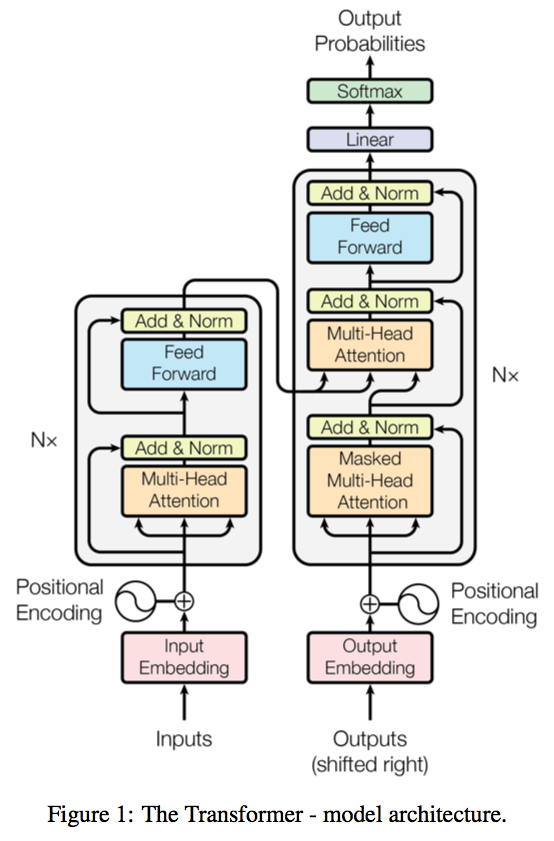
\includegraphics[width=0.35\linewidth,keepaspectratio]{transformer}
			
			{\tiny From ``Attention is all you need'' paper by Vaswani, et al., 2017}
			\end{center}		

			Thats' it \ldots
			
\end{frame}

%%%%%%%%%%%%%%%%%%%%%%%%%%%%%%%%%%%%%%%%%%%%%%%%%%%%%%%%%%%
\begin{frame}[fragile]\frametitle{Assuming Familiarity with \ldots}

\begin{itemize}
\item Linear Algebra: Vectors, Matrices
\item Calculus: Gradient Descent
\item Statistics: Distributions
\item Machine Learning: Supervised, Softmax
\item Deep Learning: Back-propagation, 
\item Natural Language Processing: Tokenization, Word Vectors, Seq2Seq (RNN, LSTM)
\end{itemize}	

\end{frame}


%%%%%%%%%%%%%%%%%%%%%%%%%%%%%%%%%%%%%%%%%%%%%%%%%%%%%%%%%%%
\begin{frame}[fragile]\frametitle{Sequence-to-Sequence (seq2seq)}

\begin{center}
See any issues with this traditional seq2seq paradigm?
\end{center}	

\end{frame}

%%%%%%%%%%%%%%%%%%%%%%%%%%%%%%%%%%%%%%%%%%%%%%%%%%%%%%%%%%%
\begin{frame}[fragile]\frametitle{Issues with recurrent models}


Linear interaction distance. %O(sequence length) steps for distant word pairs to interact means:

\begin{itemize}
\item Hard to learn long-distance dependencies (because of vanishing gradient problems!)
\item Linear order of words is ``baked in''; not necessarily the  right way to think about sentences \ldots Meaning sentence structure of one language may not be correspondingly same as order in the other language.
\end{itemize}	 

\begin{center}
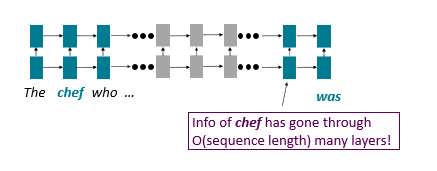
\includegraphics[width=\linewidth,keepaspectratio]{bert35}
\end{center}	

 
% {\tiny (Ref: Language \& Machine Learning - John Hewitt)}
\end{frame}

%%%%%%%%%%%%%%%%%%%%%%%%%%%%%%%%%%%%%%%%%%%%%%%%%%%%%%%%%%%
\begin{frame}[fragile]\frametitle{Issues with recurrent models}

Lack of parallelizability. %Forward and backward passes have O(sequence length) unparallelizable operations

\begin{itemize}
\item GPUs can perform a bunch of independent computations at once!
\item But future RNN hidden states can’t be computed in full before past RNN
hidden states have been computed
\item Inhibits training on very large datasets!
\end{itemize}	 

\begin{center}
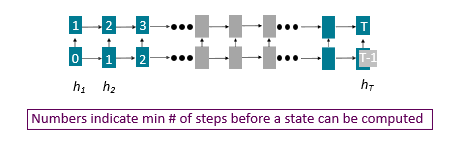
\includegraphics[width=\linewidth,keepaspectratio]{bert36}
\end{center}	

 
% {\tiny (Ref: Language \& Machine Learning - John Hewitt)}
\end{frame}

%%%%%%%%%%%%%%%%%%%%%%%%%%%%%%%%%%%%%%%%%%%%%%%%%%%%%%%%%%%
\begin{frame}[fragile]\frametitle{Then?}

If not recurrence, then what? How about word windows? Word window models aggregate local contexts

\begin{itemize}
\item Also known as 1D convolution
\item Number of unparallelizable operations not tied to sequence length!
\end{itemize}	 

\begin{center}
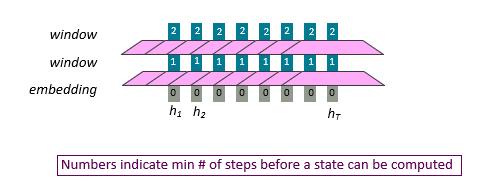
\includegraphics[width=\linewidth,keepaspectratio]{bert37}
\end{center}	

 
% {\tiny (Ref: Language \& Machine Learning - John Hewitt)}
\end{frame}

%%%%%%%%%%%%%%%%%%%%%%%%%%%%%%%%%%%%%%%%%%%%%%%%%%%%%%%%%%%
\begin{frame}[fragile]\frametitle{Then?}

What about long-distance dependencies?

\begin{itemize}
\item Stacking word window layers allows interaction between farther words
\item But if your sequences are too long, you’ll just ignore long-distance context

\end{itemize}	 

\begin{center}
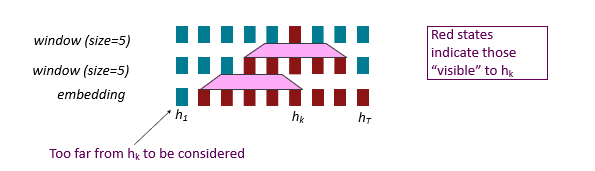
\includegraphics[width=\linewidth,keepaspectratio]{bert38}
\end{center}	

 
% {\tiny (Ref: Language \& Machine Learning - John Hewitt)}
\end{frame}

%%%%%%%%%%%%%%%%%%%%%%%%%%%%%%%%%%%%%%%%%%%%%%%%%%%%%%%%%%%
\begin{frame}[fragile]\frametitle{Attention}

If not recurrence, then what? How about attention?

\begin{itemize}
\item Attention treats each word’s representation as a query to access and  incorporate information from a set of values.
\item We saw attention from the decoder to the encoder; today we’ll think about
attention within a single sentence.
\item If attention gives us access to any state… maybe we can just use attention and don’t need the RNN?
%\item Number of unparallelizable operations not tied to sequence length.
\item All words interact at every layer!

\end{itemize}	 

\begin{center}
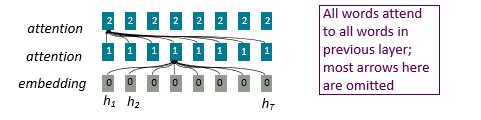
\includegraphics[width=\linewidth,keepaspectratio]{bert39}
\end{center}	

 
% {\tiny (Ref: Language \& Machine Learning - John Hewitt)}
\end{frame}



\section[Trs]{Transformer}
%%%%%%%%%%%%%%%%%%%%%%%%%%%%%%%%%%%%%%%%%%%%%%%%%%%%%%%%%%%%%%%%%%%%%%%%%%%%%%%%%%
\begin{frame}[fragile]\frametitle{}
\begin{center}
{\Large Transformer \\ \small Attention is all you need}
\end{center}
\end{frame}


%%%%%%%%%%%%%%%%%%%%%%%%%%%%%%%%%%%%%%%%%%%%%%%%%%%%%%%%%%%
\begin{frame}[fragile]\frametitle{Popularity}

Masking the future in self-attention

\begin{center}
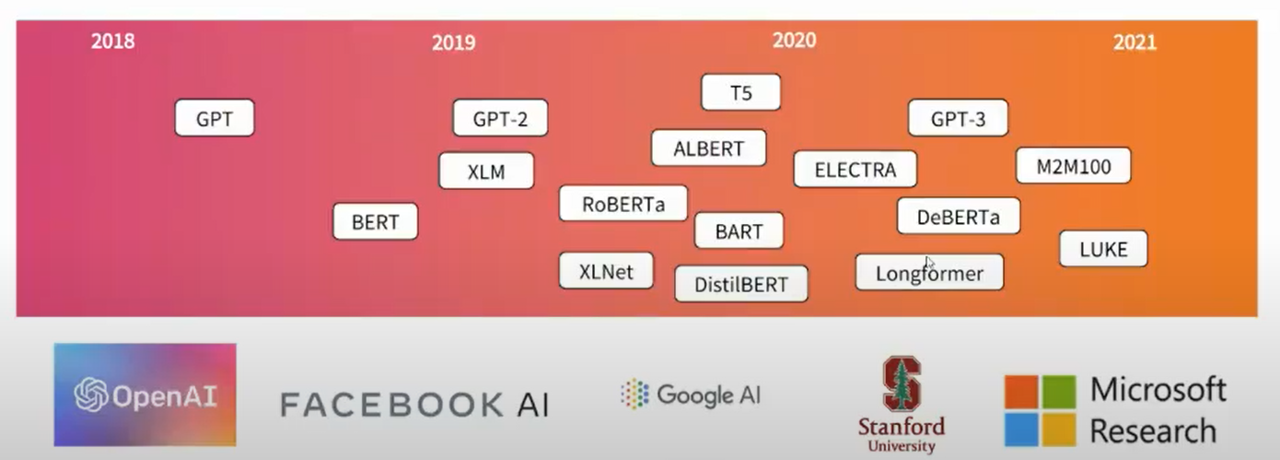
\includegraphics[width=\linewidth,keepaspectratio]{bert50}
\end{center}	

 
% {\tiny (Ref: Niels Rogge on Huggingface contributions)}
\end{frame}


%%%%%%%%%%%%%%%%%%%%%%%%%%%%%%%%%%%%%%%%%%%%%%%%%%%%%%%%%%%
\begin{frame}[fragile]\frametitle{Transformers}


\begin{itemize}
\item The Transformer  is a model that uses attention to boost the speed with which seq2seq with attention models can be trained. The biggest benefit, however, comes from how The Transformer lends itself to parallelization. We will break it apart and look at how it functions.
\item In its heart it contains an encoding component, a decoding component, and connections between them.
\end{itemize}	 

\begin{center}
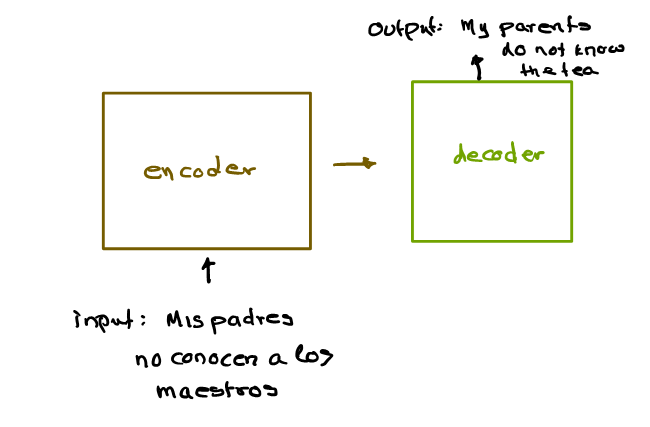
\includegraphics[width=0.6\linewidth,keepaspectratio]{bert51}
\end{center}	

\end{frame}


%%%%%%%%%%%%%%%%%%%%%%%%%%%%%%%%%%%%%%%%%%%%%%%%%%%%%%%%%%%
\begin{frame}[fragile]\frametitle{Transformers}
\begin{columns}
    \begin{column}[T]{0.5\linewidth}
      \begin{itemize}
			\item The encoding is a stack of encoders.
			\item The original paper stacks six of them on top of each other – there’s nothing magical about the number six, one can definitely experiment with other arrangements). 
			\item The decoding is a stack of decoders of the same number.
			\end{itemize}
		\end{column}
    \begin{column}[T]{0.5\linewidth}
		
			\begin{center}
			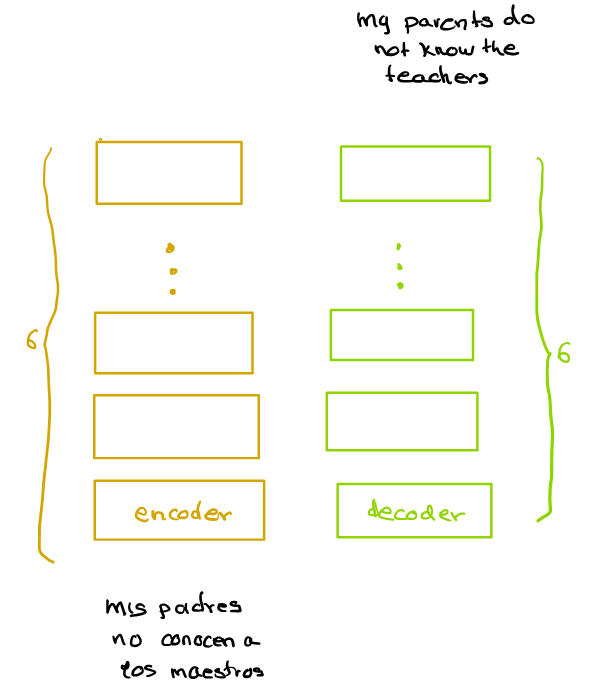
\includegraphics[width=0.8\linewidth,keepaspectratio]{bert52}
			\end{center}

    \end{column}
  \end{columns}
\end{frame}


%%%%%%%%%%%%%%%%%%%%%%%%%%%%%%%%%%%%%%%%%%%%%%%%%%%%%%%%%%%
\begin{frame}[fragile]\frametitle{Transformers}
\begin{columns}
    \begin{column}[T]{0.5\linewidth}
     The encoder’s inputs goes through a self-attention layer – a layer that helps the encoder look at other words in the input sentence as it encodes a specific word.  
		\end{column}
    \begin{column}[T]{0.5\linewidth}
		The decoder has both those layers, but between them is an attention layer that helps the decoder focus on relevant parts of the input sentence (similar what attention does in seq2seq models).
    \end{column}
  \end{columns}
	
			\begin{center}
			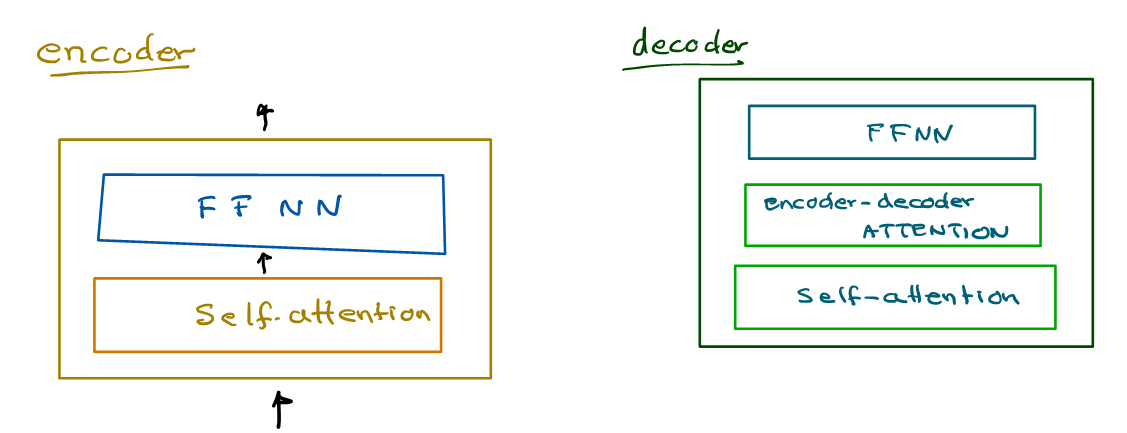
\includegraphics[width=0.8\linewidth,keepaspectratio]{bert53}
			\end{center}
			
\end{frame}

%%%%%%%%%%%%%%%%%%%%%%%%%%%%%%%%%%%%%%%%%%%%%%%%%%%%%%%%%%%
\begin{frame}[fragile]\frametitle{Transformers}
\begin{columns}
    \begin{column}[T]{0.5\linewidth}
			\begin{center}
			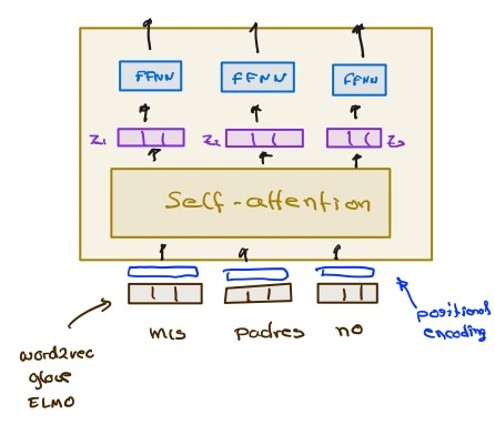
\includegraphics[width=0.8\linewidth,keepaspectratio]{bert58}
			\end{center}		
		\end{column}
    \begin{column}[T]{0.5\linewidth}
      \begin{itemize}
			\item A key property of the Transformer, which is that the word in each position flows through its own path in the encoder. There are dependencies between these paths in the self-attention layer. 
			\item The feed-forward layer does not have those dependencies, Therefore, the various paths can be executed in parallel while flowing through the feed-forward layer.
			\end{itemize}
    \end{column}
  \end{columns}
			
\end{frame}

%%%%%%%%%%%%%%%%%%%%%%%%%%%%%%%%%%%%%%%%%%%%%%%%%%%%%%%%%%%
\begin{frame}[fragile]\frametitle{Transformers}
Patrick was not late for class because {\bf he} is a responsible student

\begin{columns}
    \begin{column}[T]{0.5\linewidth}
			\begin{center}
			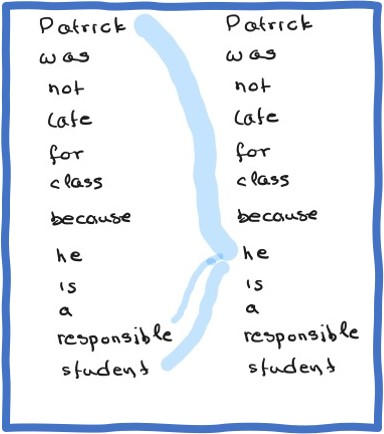
\includegraphics[width=\linewidth,keepaspectratio]{bert54}
			\end{center}		
		\end{column}
    \begin{column}[T]{0.5\linewidth}
      \begin{itemize}
			\item What does ``he'' in this sentence refer to? Is it referring to the class or to the student? It's a simple question to a human, but not as simple to an algorithm.
			\item When the model is processing the word ``he'', self-attention allows it to associate ``he'' with ``Patrick''.
			\end{itemize}
    \end{column}
  \end{columns}
			
\end{frame}

%%%%%%%%%%%%%%%%%%%%%%%%%%%%%%%%%%%%%%%%%%%%%%%%%%%%%%%%%%%
\begin{frame}[fragile]\frametitle{Transformers}
	\begin{center}
	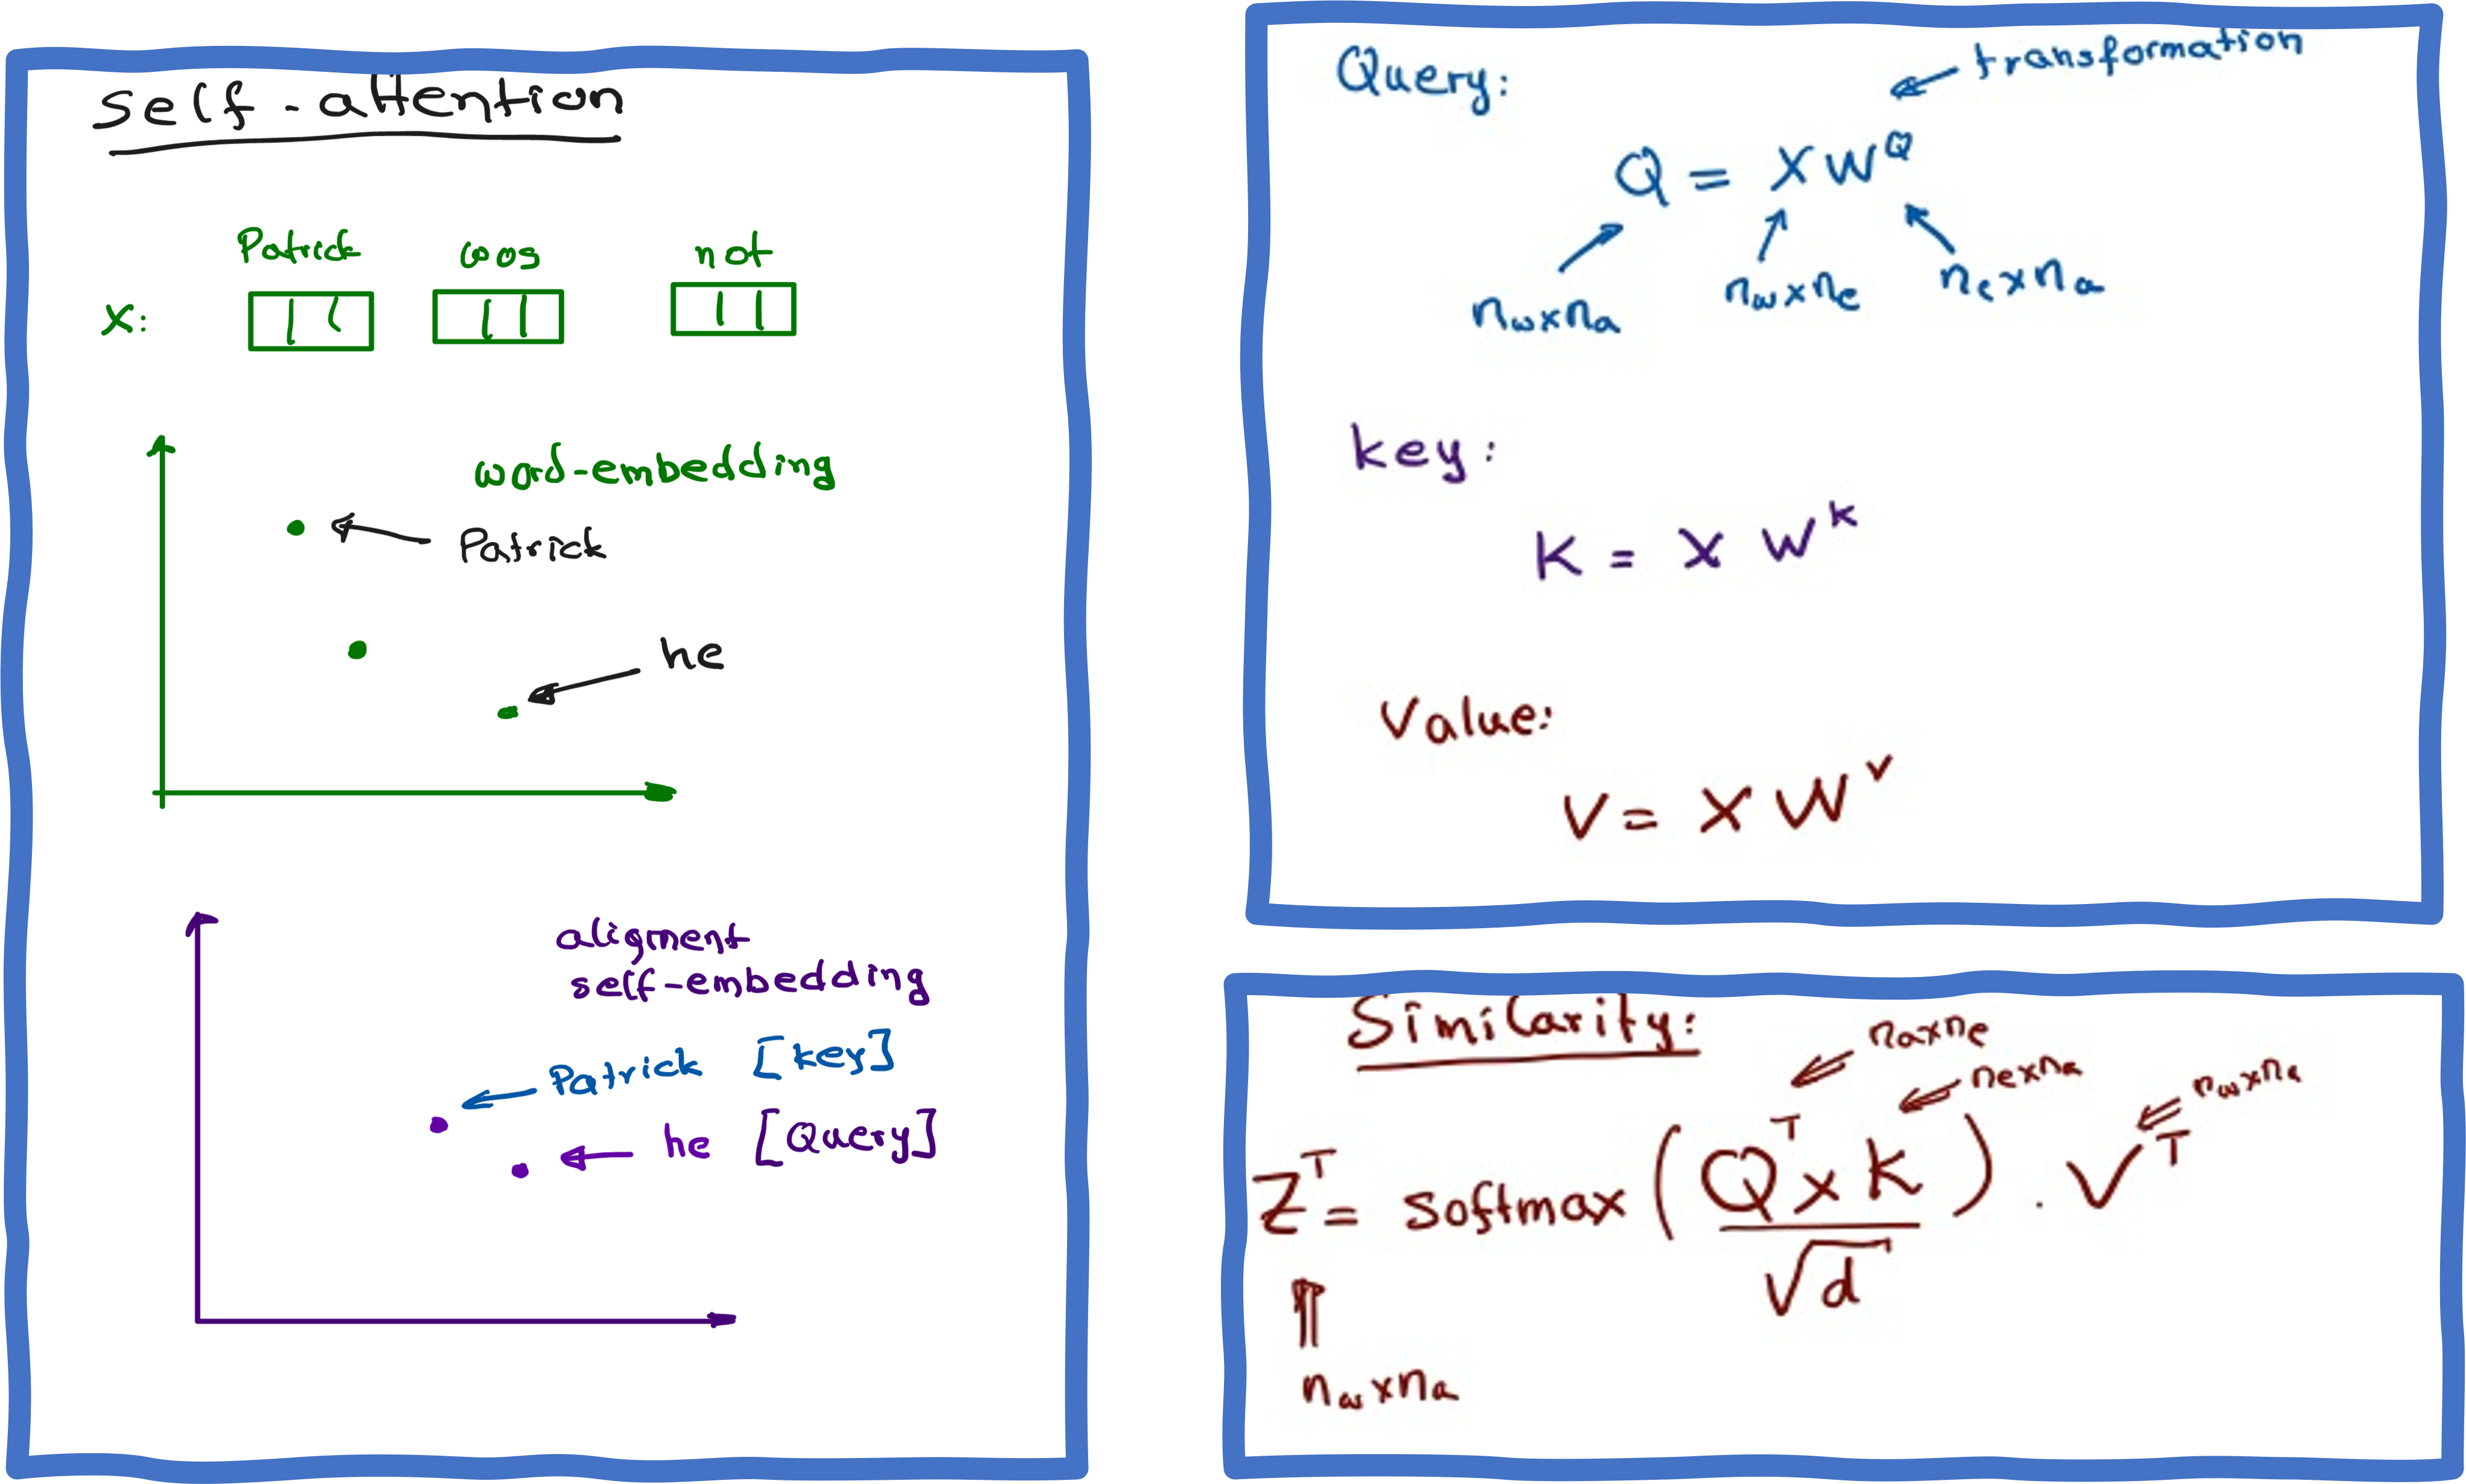
\includegraphics[width=\linewidth,keepaspectratio]{bert55}
	\end{center}	
\end{frame}

%%%%%%%%%%%%%%%%%%%%%%%%%%%%%%%%%%%%%%%%%%%%%%%%%%%%%%%%%%%
\begin{frame}[fragile]\frametitle{Transformers}

\begin{columns}
    \begin{column}[T]{0.5\linewidth}
			\begin{center}
			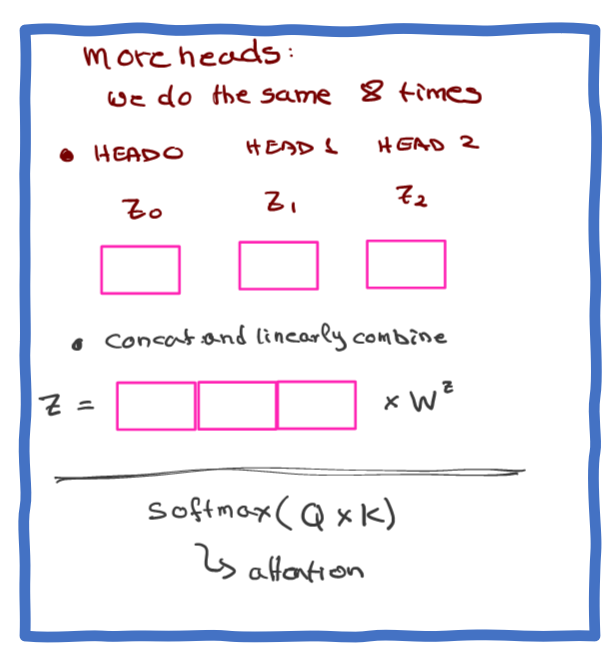
\includegraphics[width=\linewidth,keepaspectratio]{bert60}
			\end{center}		
		\end{column}
    \begin{column}[T]{0.5\linewidth}
		In the same fashion as CNN that we need more than one filter, transformers add a mechanism called ``multi-headed'' attention. This improves the performance of the attention layer in two ways:

      \begin{itemize}
			\item It expands the model's ability to focus on different positions.
			\item It gives the attention layer multiple ``representation subspaces''
			\end{itemize}
    \end{column}
  \end{columns}
			
\end{frame}

%%%%%%%%%%%%%%%%%%%%%%%%%%%%%%%%%%%%%%%%%%%%%%%%%%%%%%%%%%%
\begin{frame}[fragile]\frametitle{Transformers}

\begin{columns}
    \begin{column}[T]{0.5\linewidth}
			\begin{center}
			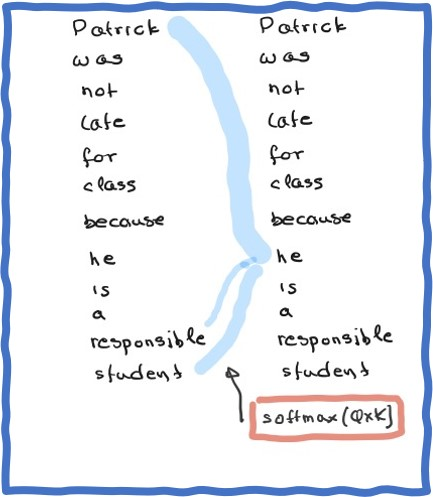
\includegraphics[width=\linewidth,keepaspectratio]{bert56}
			\end{center}		
		\end{column}
    \begin{column}[T]{0.5\linewidth}
As we encode the word ”he", one attention head is focusing most on ``Patrick'', while another is focusing on ``student'' -- in a sense, the model's representation of the word ``he'' combines the representations of both ``Patrick'' and ``stduent''.

    \end{column}
  \end{columns}
			
\end{frame}

%%%%%%%%%%%%%%%%%%%%%%%%%%%%%%%%%%%%%%%%%%%%%%%%%%%%%%%%%%%
\begin{frame}[fragile]\frametitle{Transformers}


			\begin{center}
			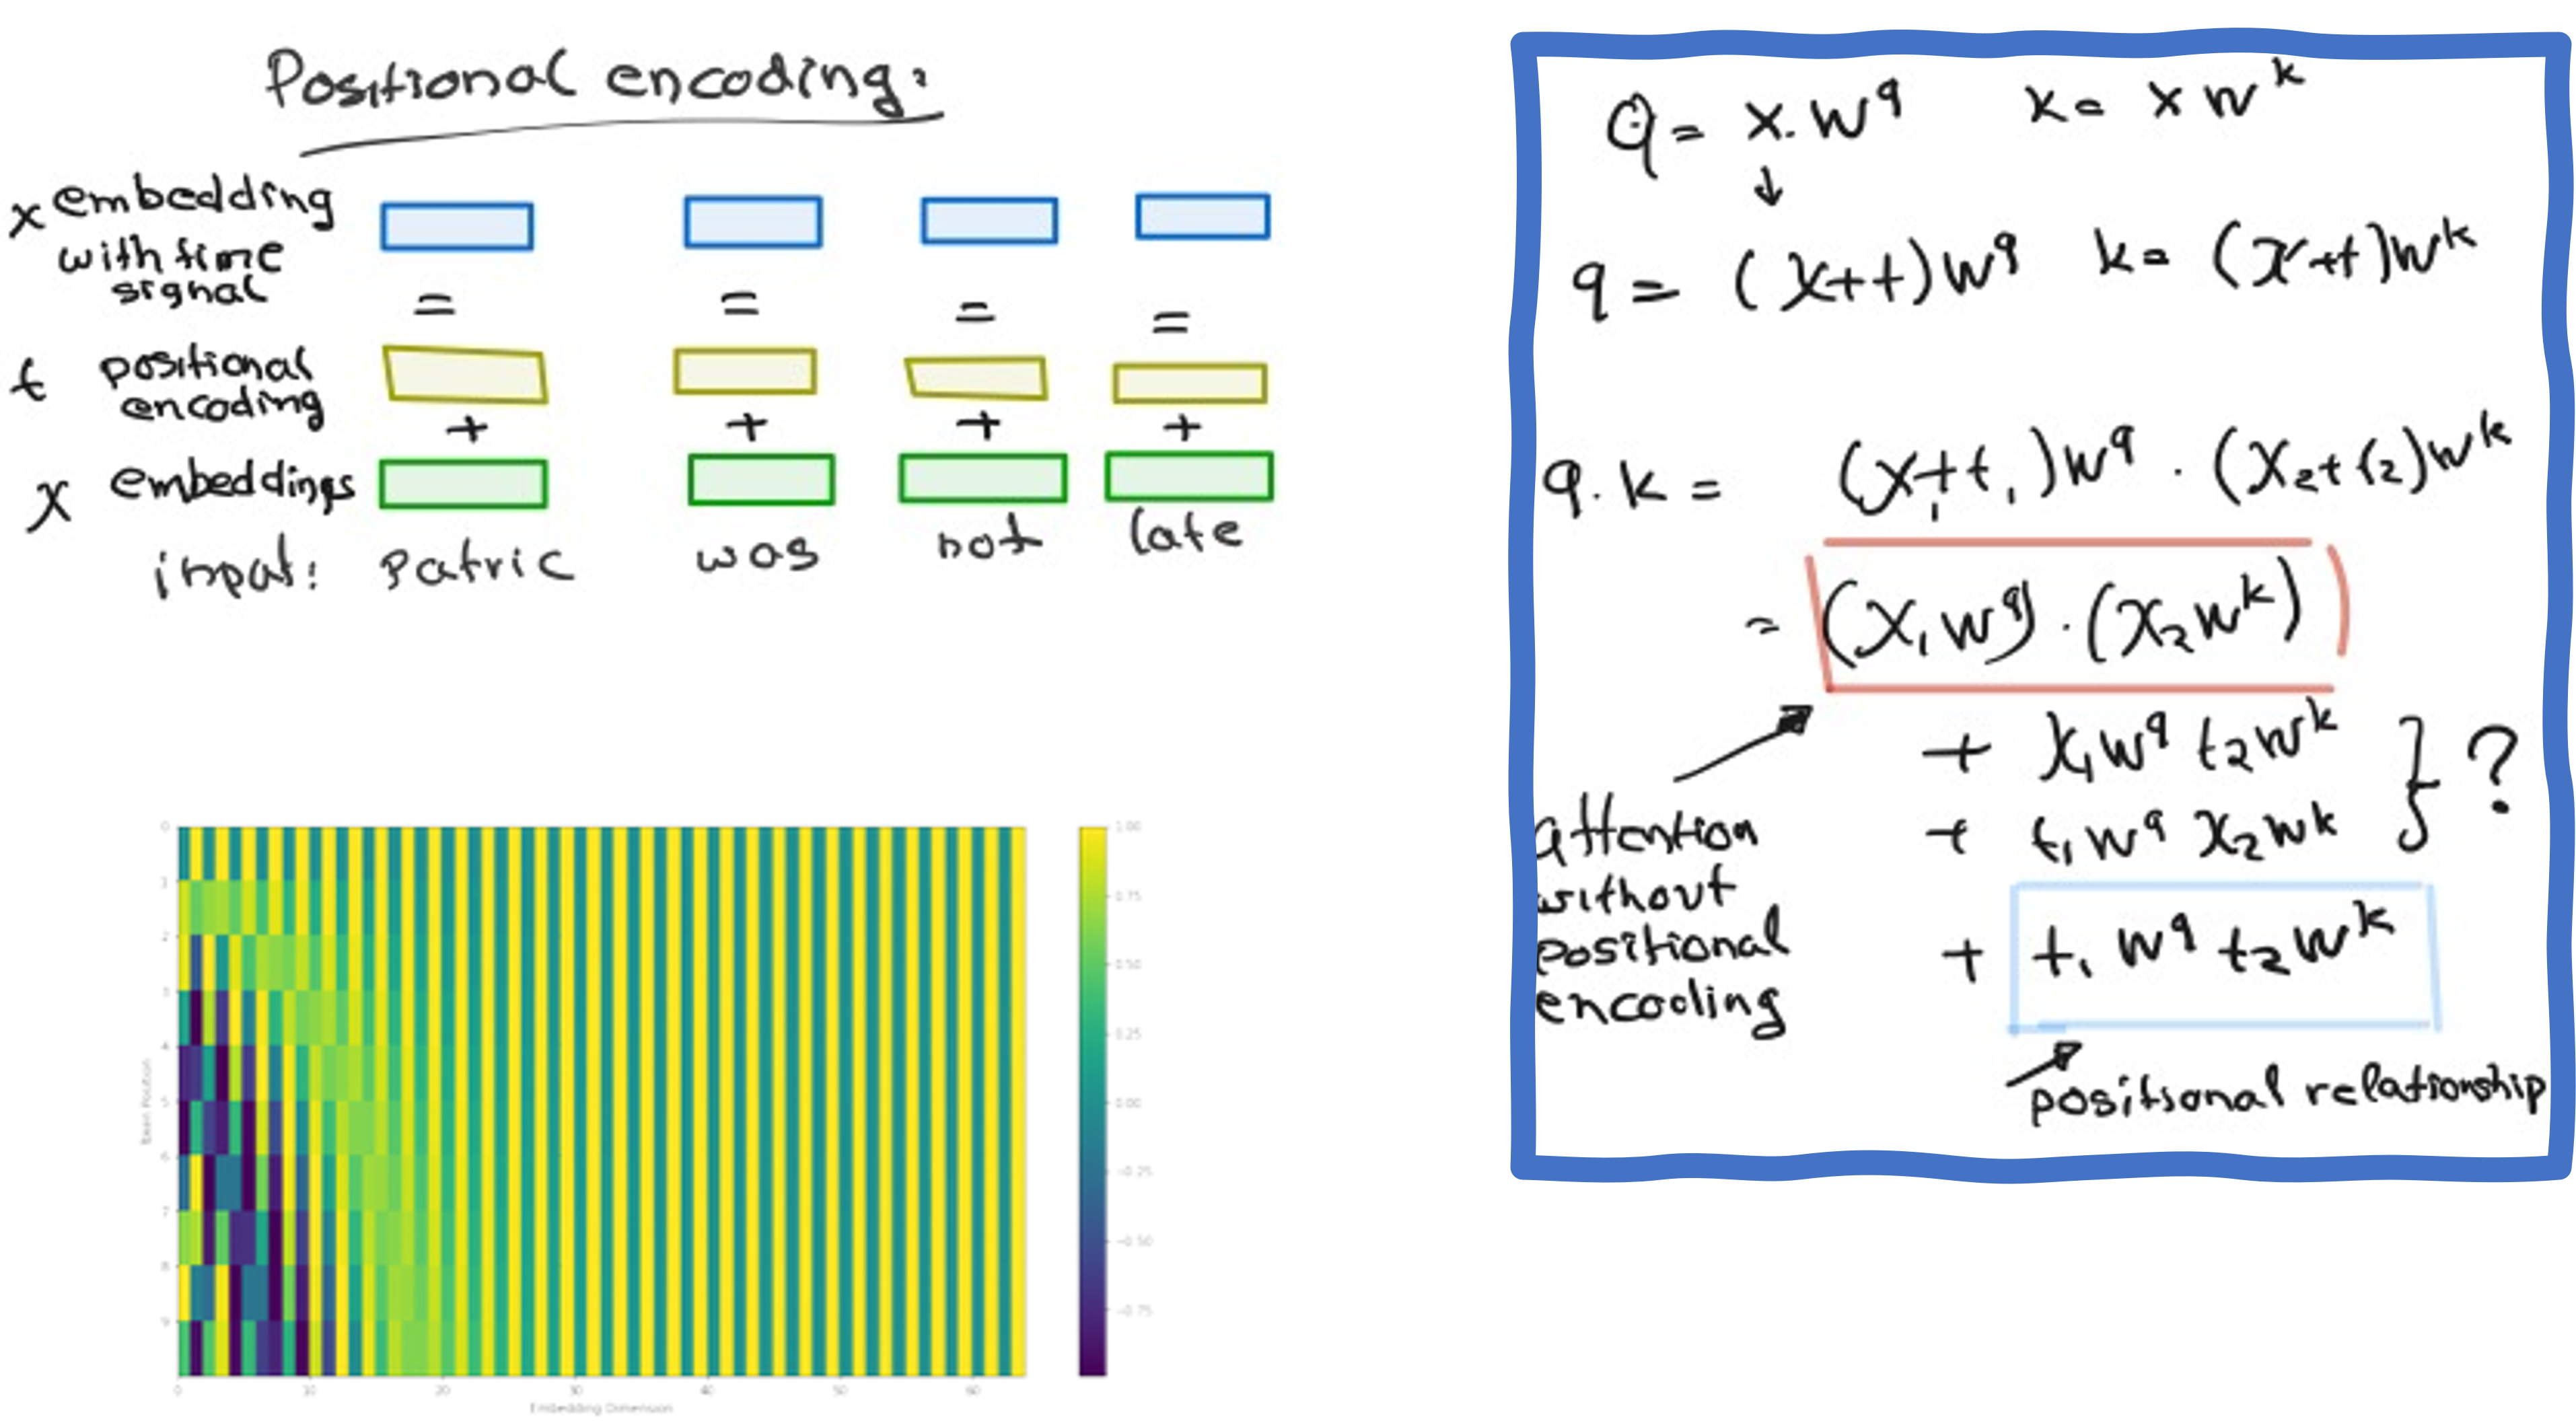
\includegraphics[width=\linewidth,keepaspectratio]{bert57}
			\end{center}		

			
\end{frame}


%%%%%%%%%%%%%%%%%%%%%%%%%%%%%%%%%%%%%%%%%%%%%%%%%%%%%%%%%%%
\begin{frame}[fragile]\frametitle{Transformers}

\begin{columns}
    \begin{column}[T]{0.5\linewidth}
			\begin{center}
			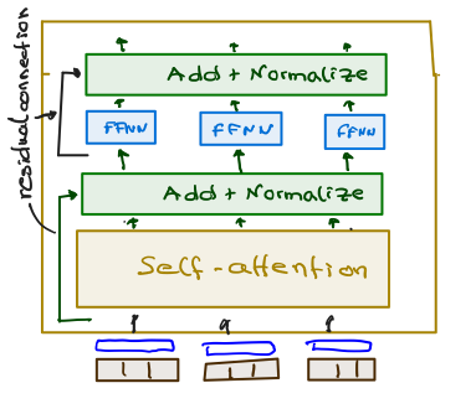
\includegraphics[width=\linewidth,keepaspectratio]{bert61}
			\end{center}		
		\end{column}
    \begin{column}[T]{0.5\linewidth}
      \begin{itemize}
			\item Details in the architecture of the encoder:
			\item Each sub-layer  in each encoder has a residual connection around it
			\item And a layer-normalization step.
			\end{itemize}
    \end{column}
  \end{columns}
			
\end{frame}

%%%%%%%%%%%%%%%%%%%%%%%%%%%%%%%%%%%%%%%%%%%%%%%%%%%%%%%%%%%
\begin{frame}[fragile]\frametitle{Transformers}


			\begin{center}
			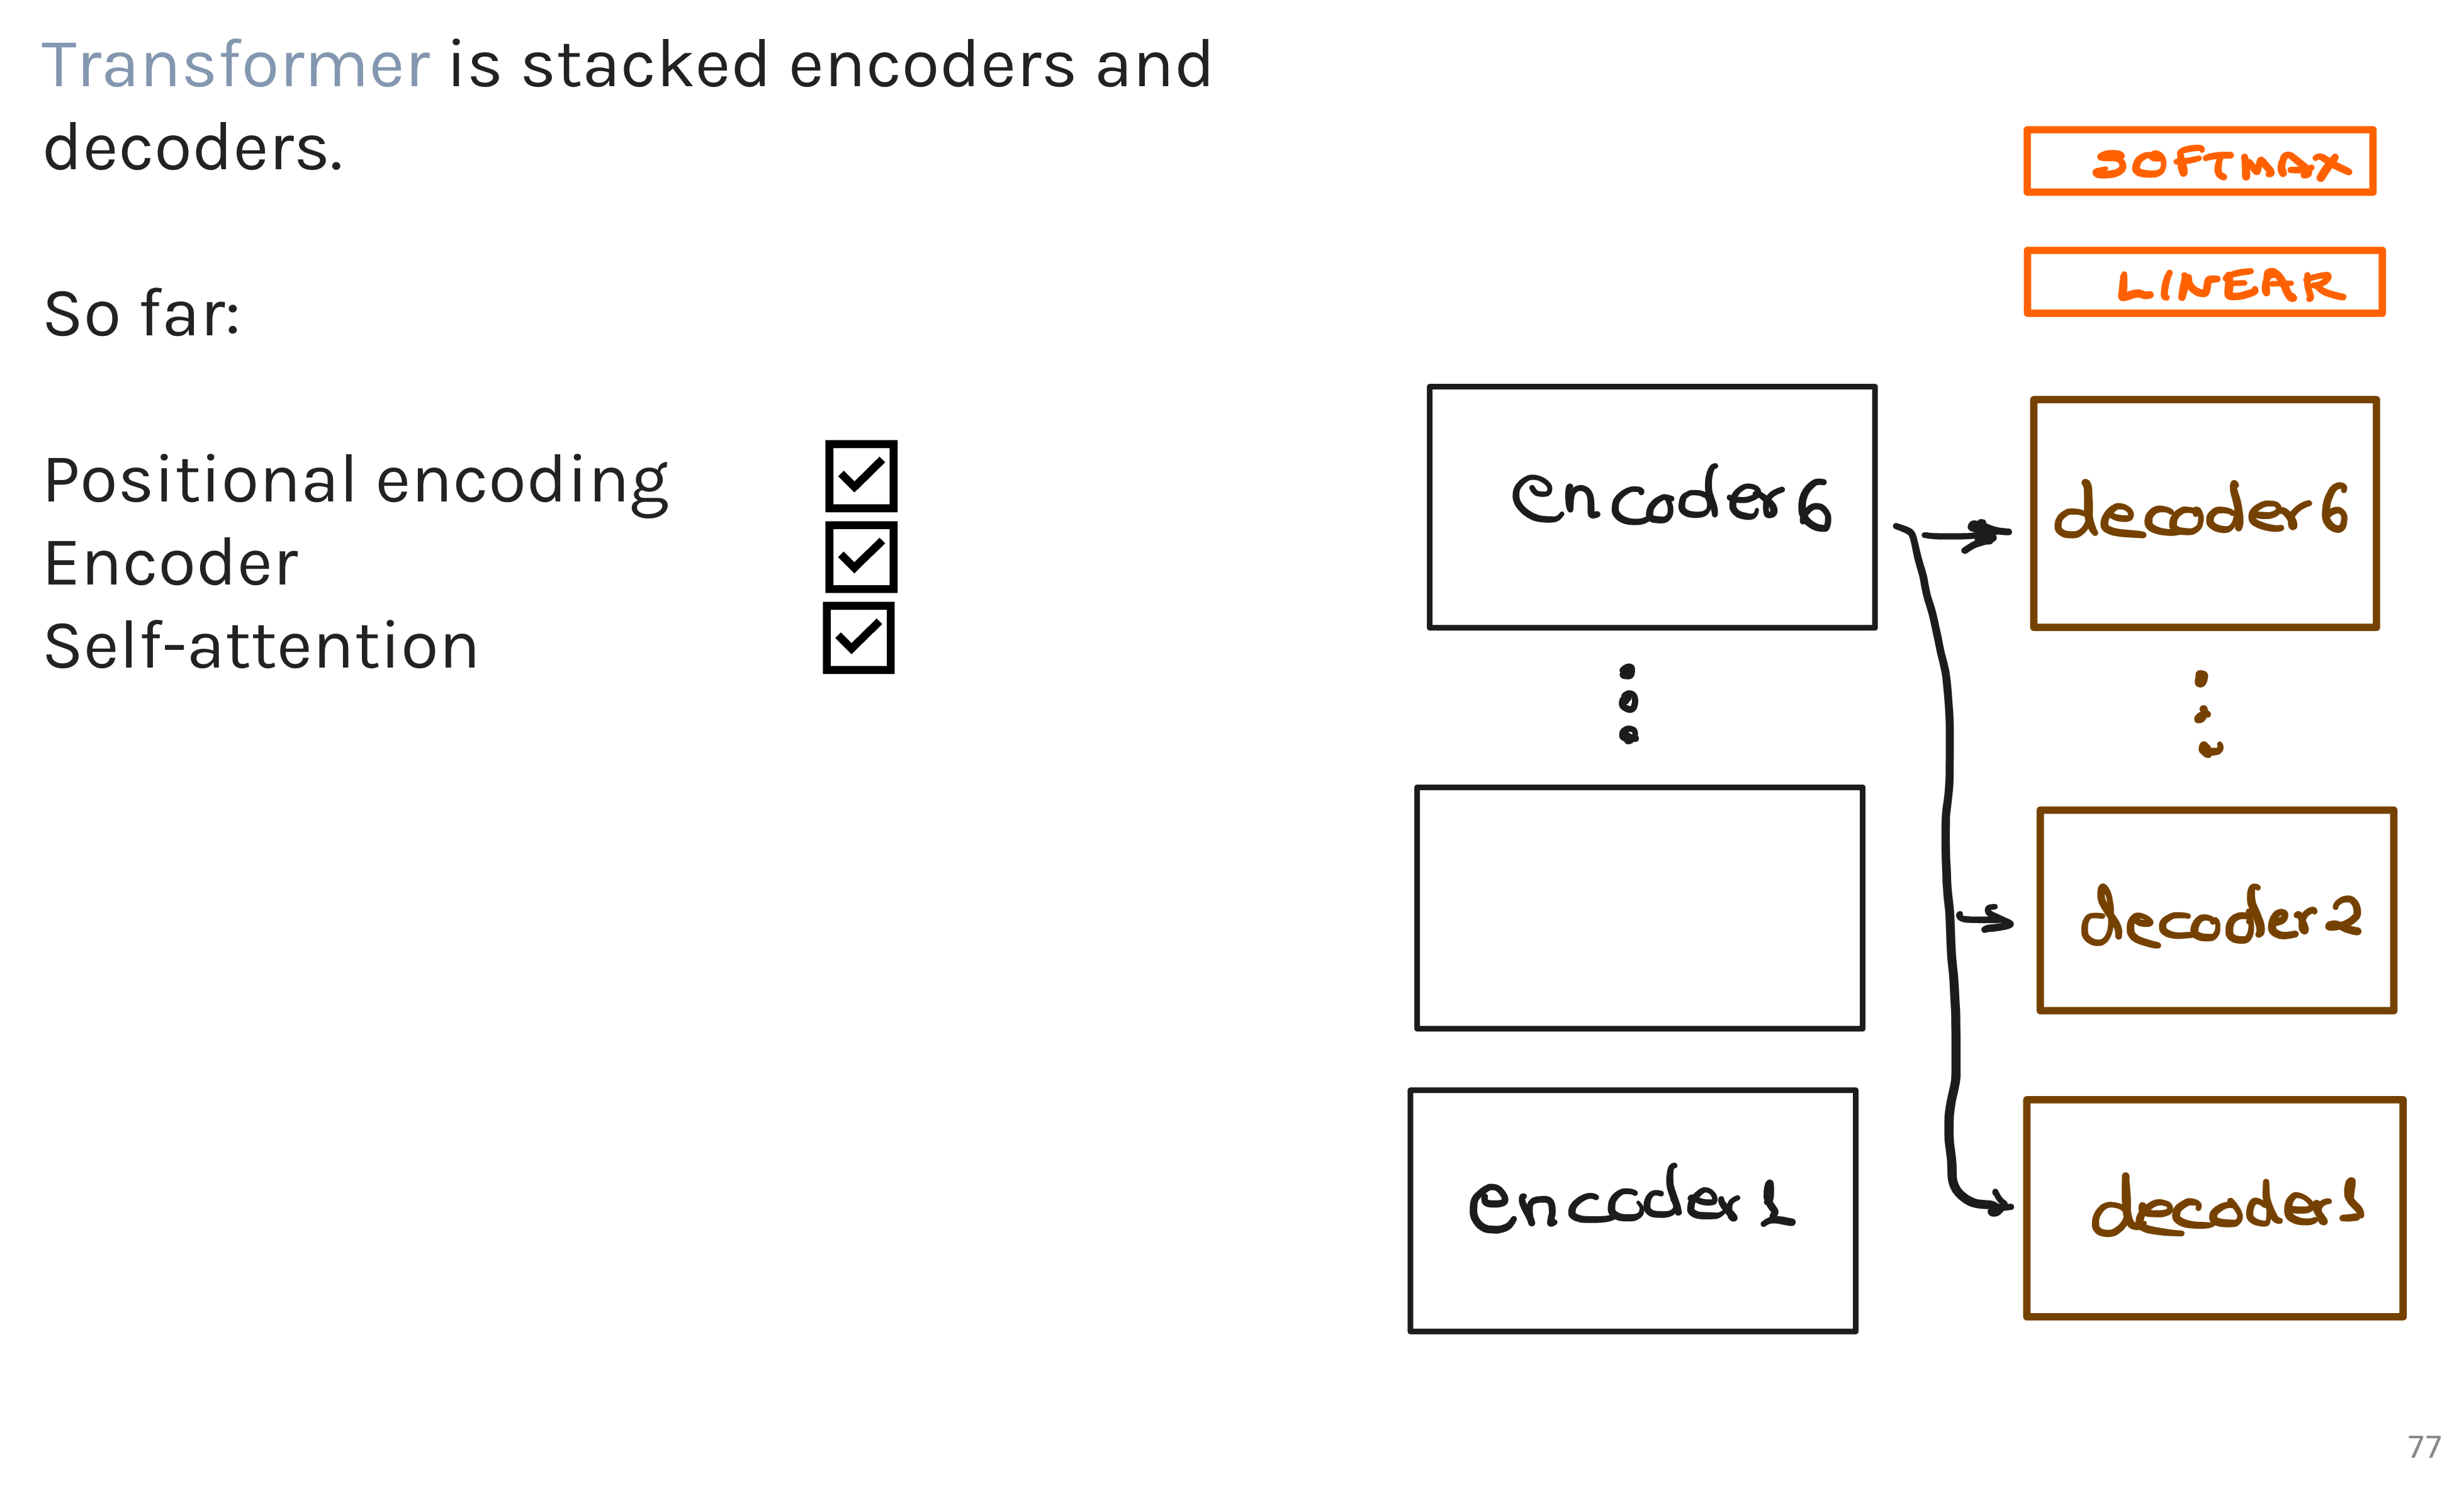
\includegraphics[width=\linewidth,keepaspectratio]{bert62}
			\end{center}		

			
\end{frame}

%%%%%%%%%%%%%%%%%%%%%%%%%%%%%%%%%%%%%%%%%%%%%%%%%%%%%%%%%%%
\begin{frame}[fragile]\frametitle{Transformers}


			\begin{center}
			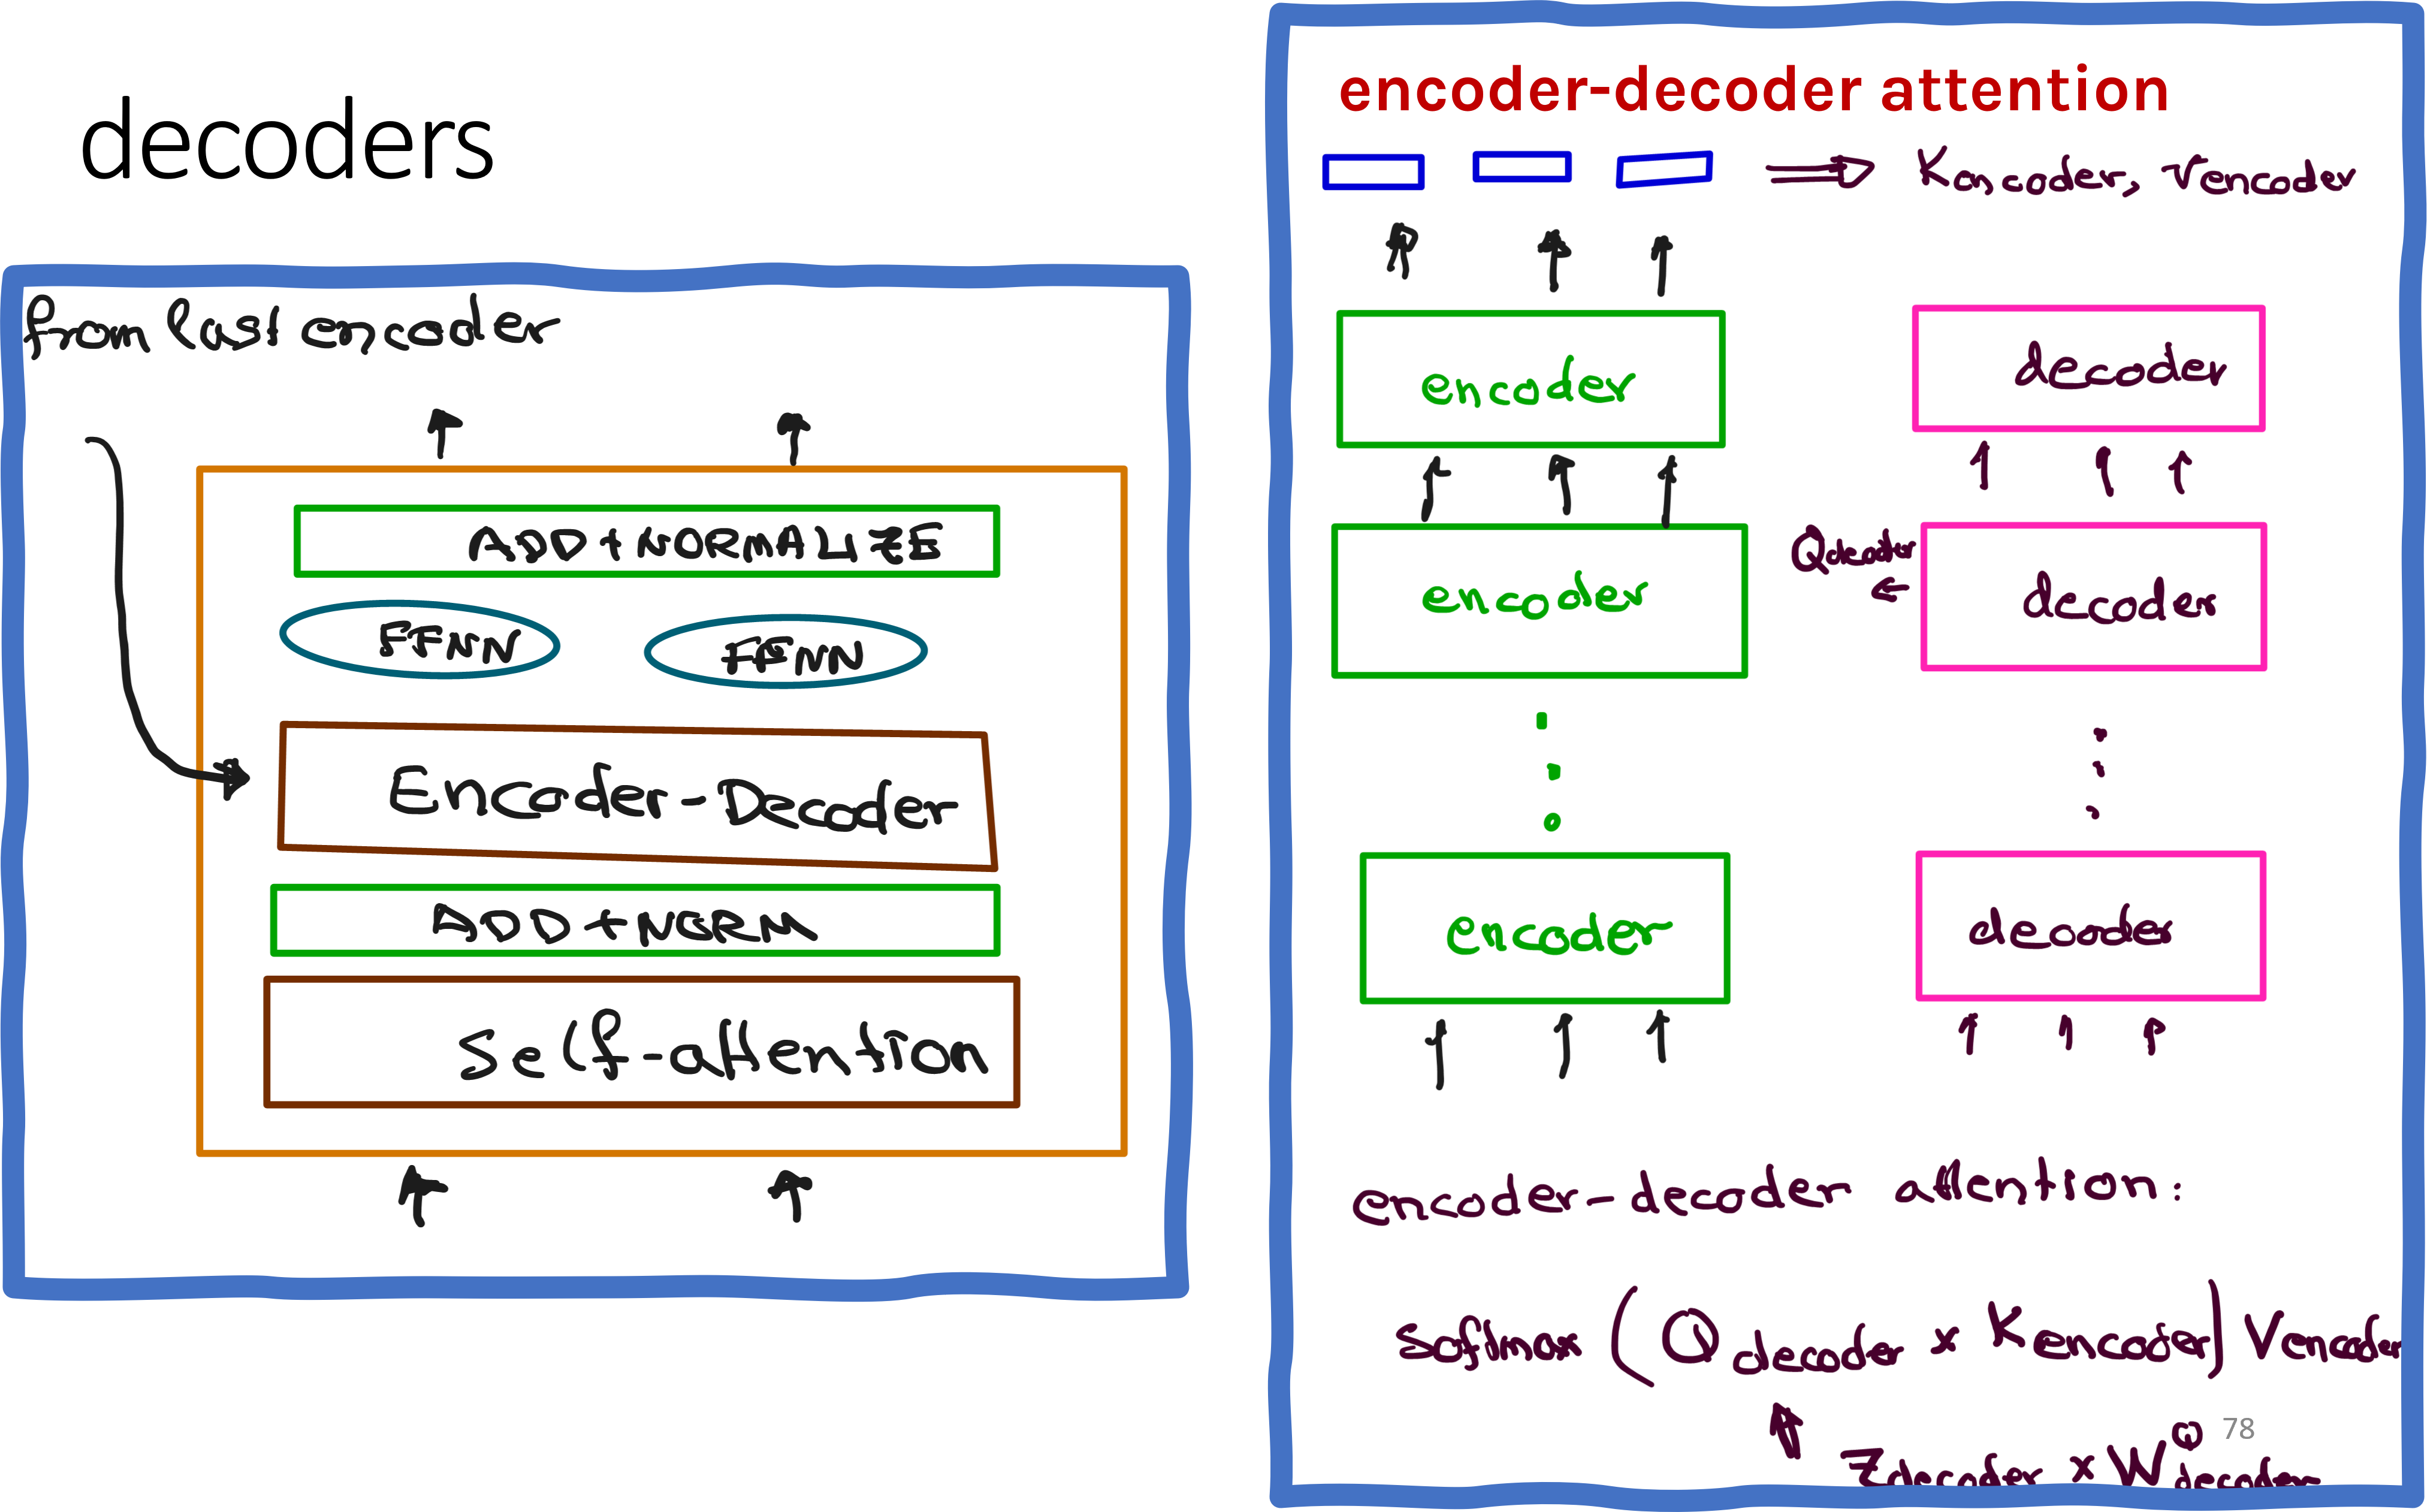
\includegraphics[width=\linewidth,keepaspectratio]{bert63}
			\end{center}		

			
\end{frame}

%%%%%%%%%%%%%%%%%%%%%%%%%%%%%%%%%%%%%%%%%%%%%%%%%%%%%%%%%%%
\begin{frame}[fragile]\frametitle{The Final Linear and Softmax Layer}


			\begin{center}
			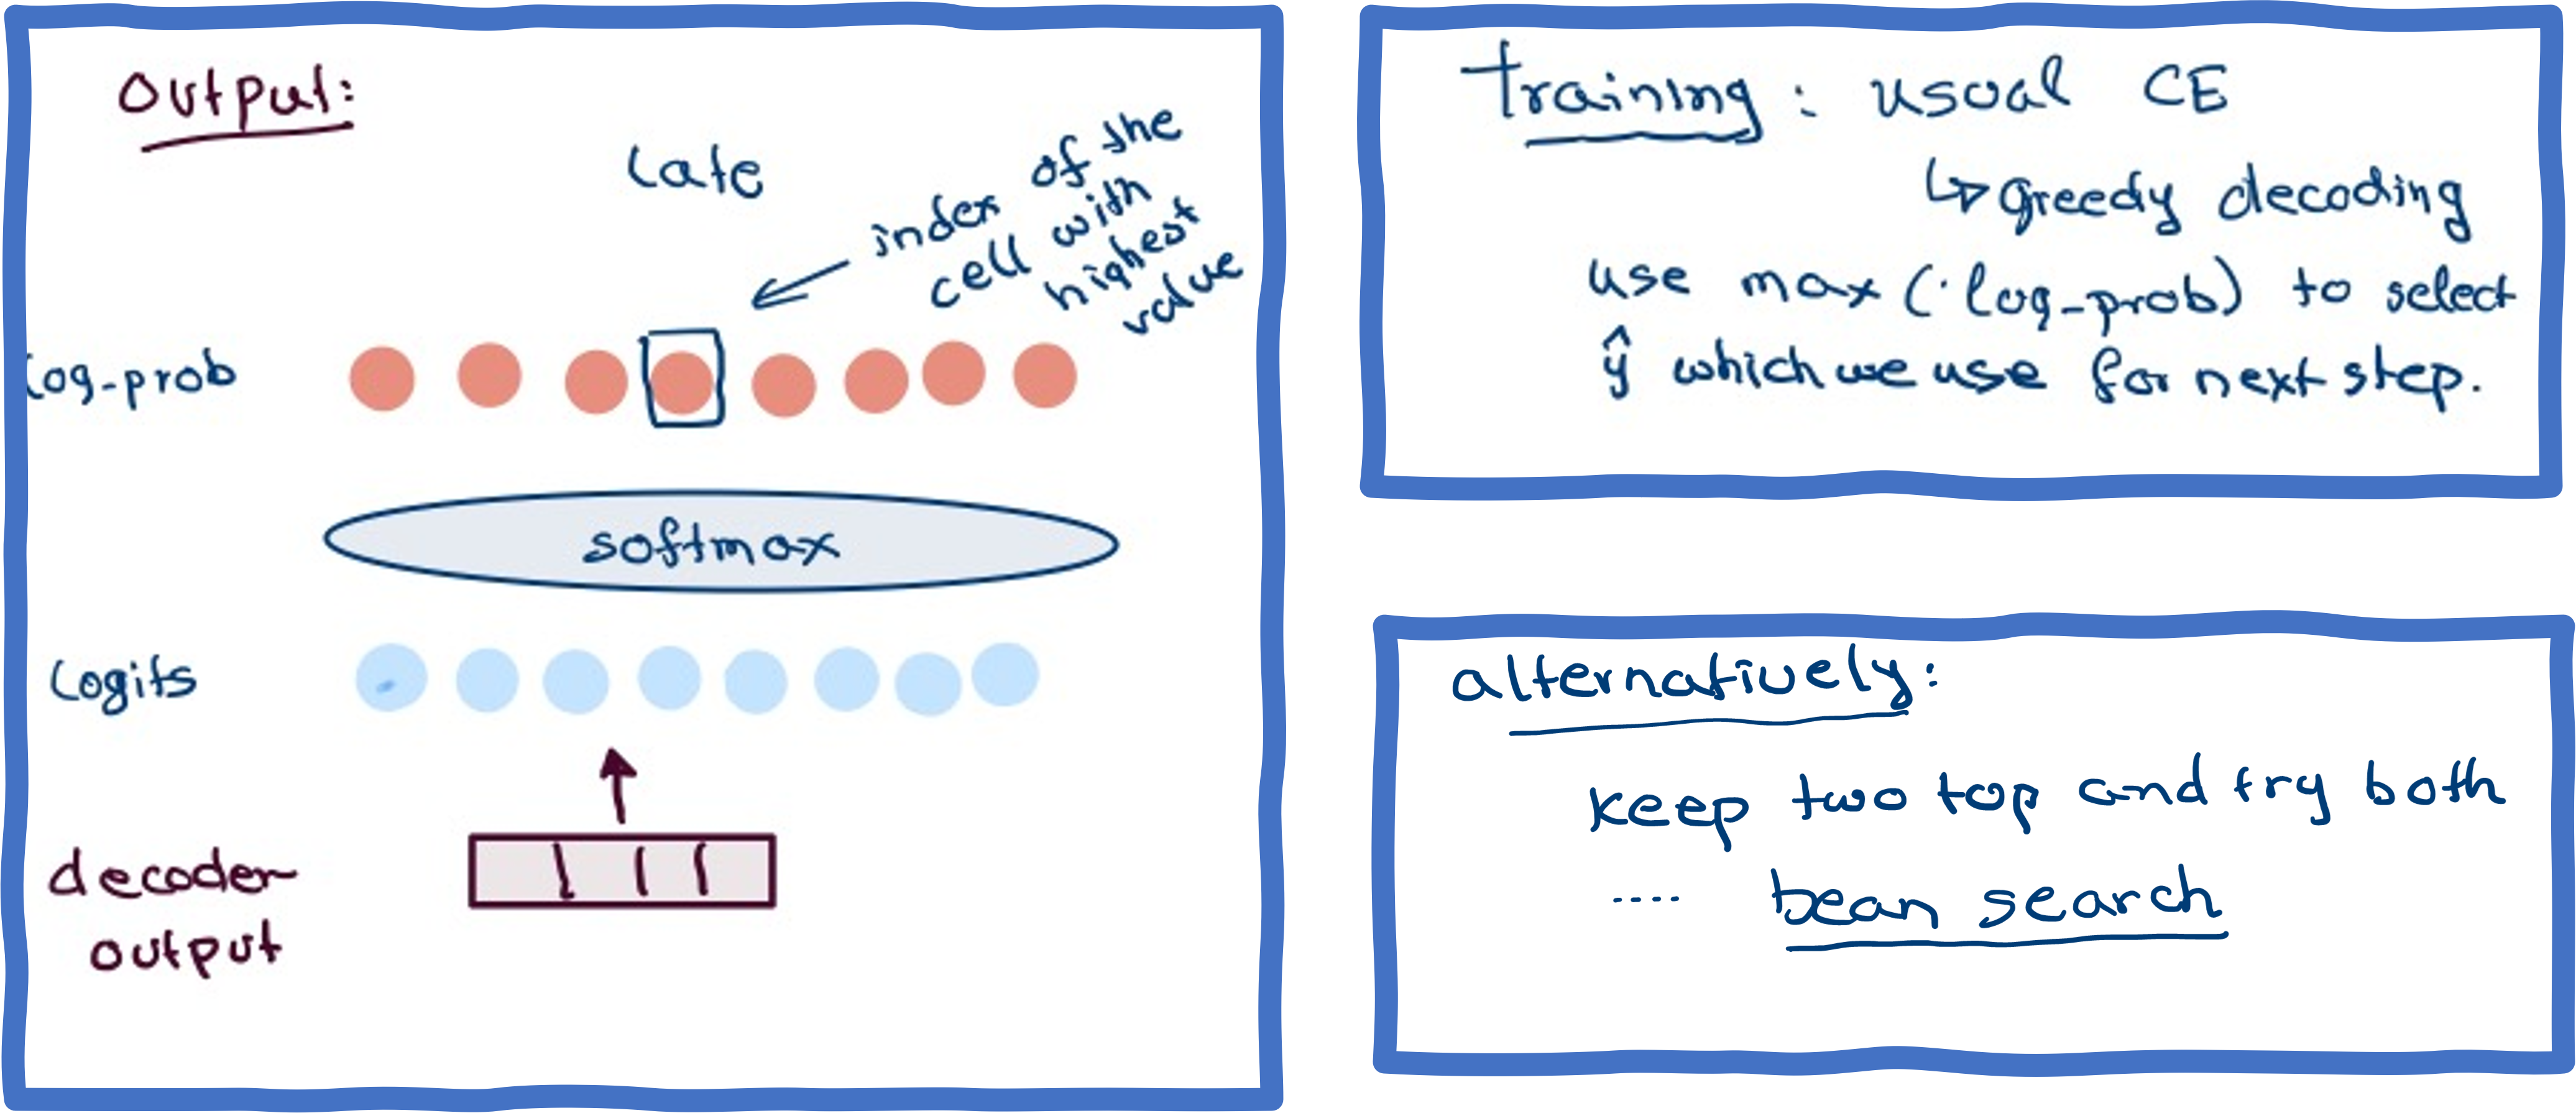
\includegraphics[width=\linewidth,keepaspectratio]{bert64}
			\end{center}		

			
\end{frame}

%%%%%%%%%%%%%%%%%%%%%%%%%%%%%%%%%%%%%%%%%%%%%%%%%%%%%%%%%%%
\begin{frame}[fragile]\frametitle{Conclusion}

Main innovations in Transformers:
\begin{itemize}
\item Positional Encoding: instead of architecture relying on sequence order, like RNNs, the Transformers store the position, making them order independent architecturally as the position is part of th data itself so that you can then have parallel processing
\item Self-attention: Weights vector, how much each word contributes, learnt by seeing many pairs, during training. Self, meaning within itself. Internal structure understanding, Encoder only.

			\end{itemize}
			
\end{frame}

% %%%%%%%%%%%%%%%%%%%%%%%%%%%%%%%%%%%%%%%%%%%%%%%%%%%%%%%%%%%
% \begin{frame}[fragile]\frametitle{Transformer Overview}

% \begin{columns}
    % \begin{column}[T]{0.5\linewidth}
			% \begin{center}
			% 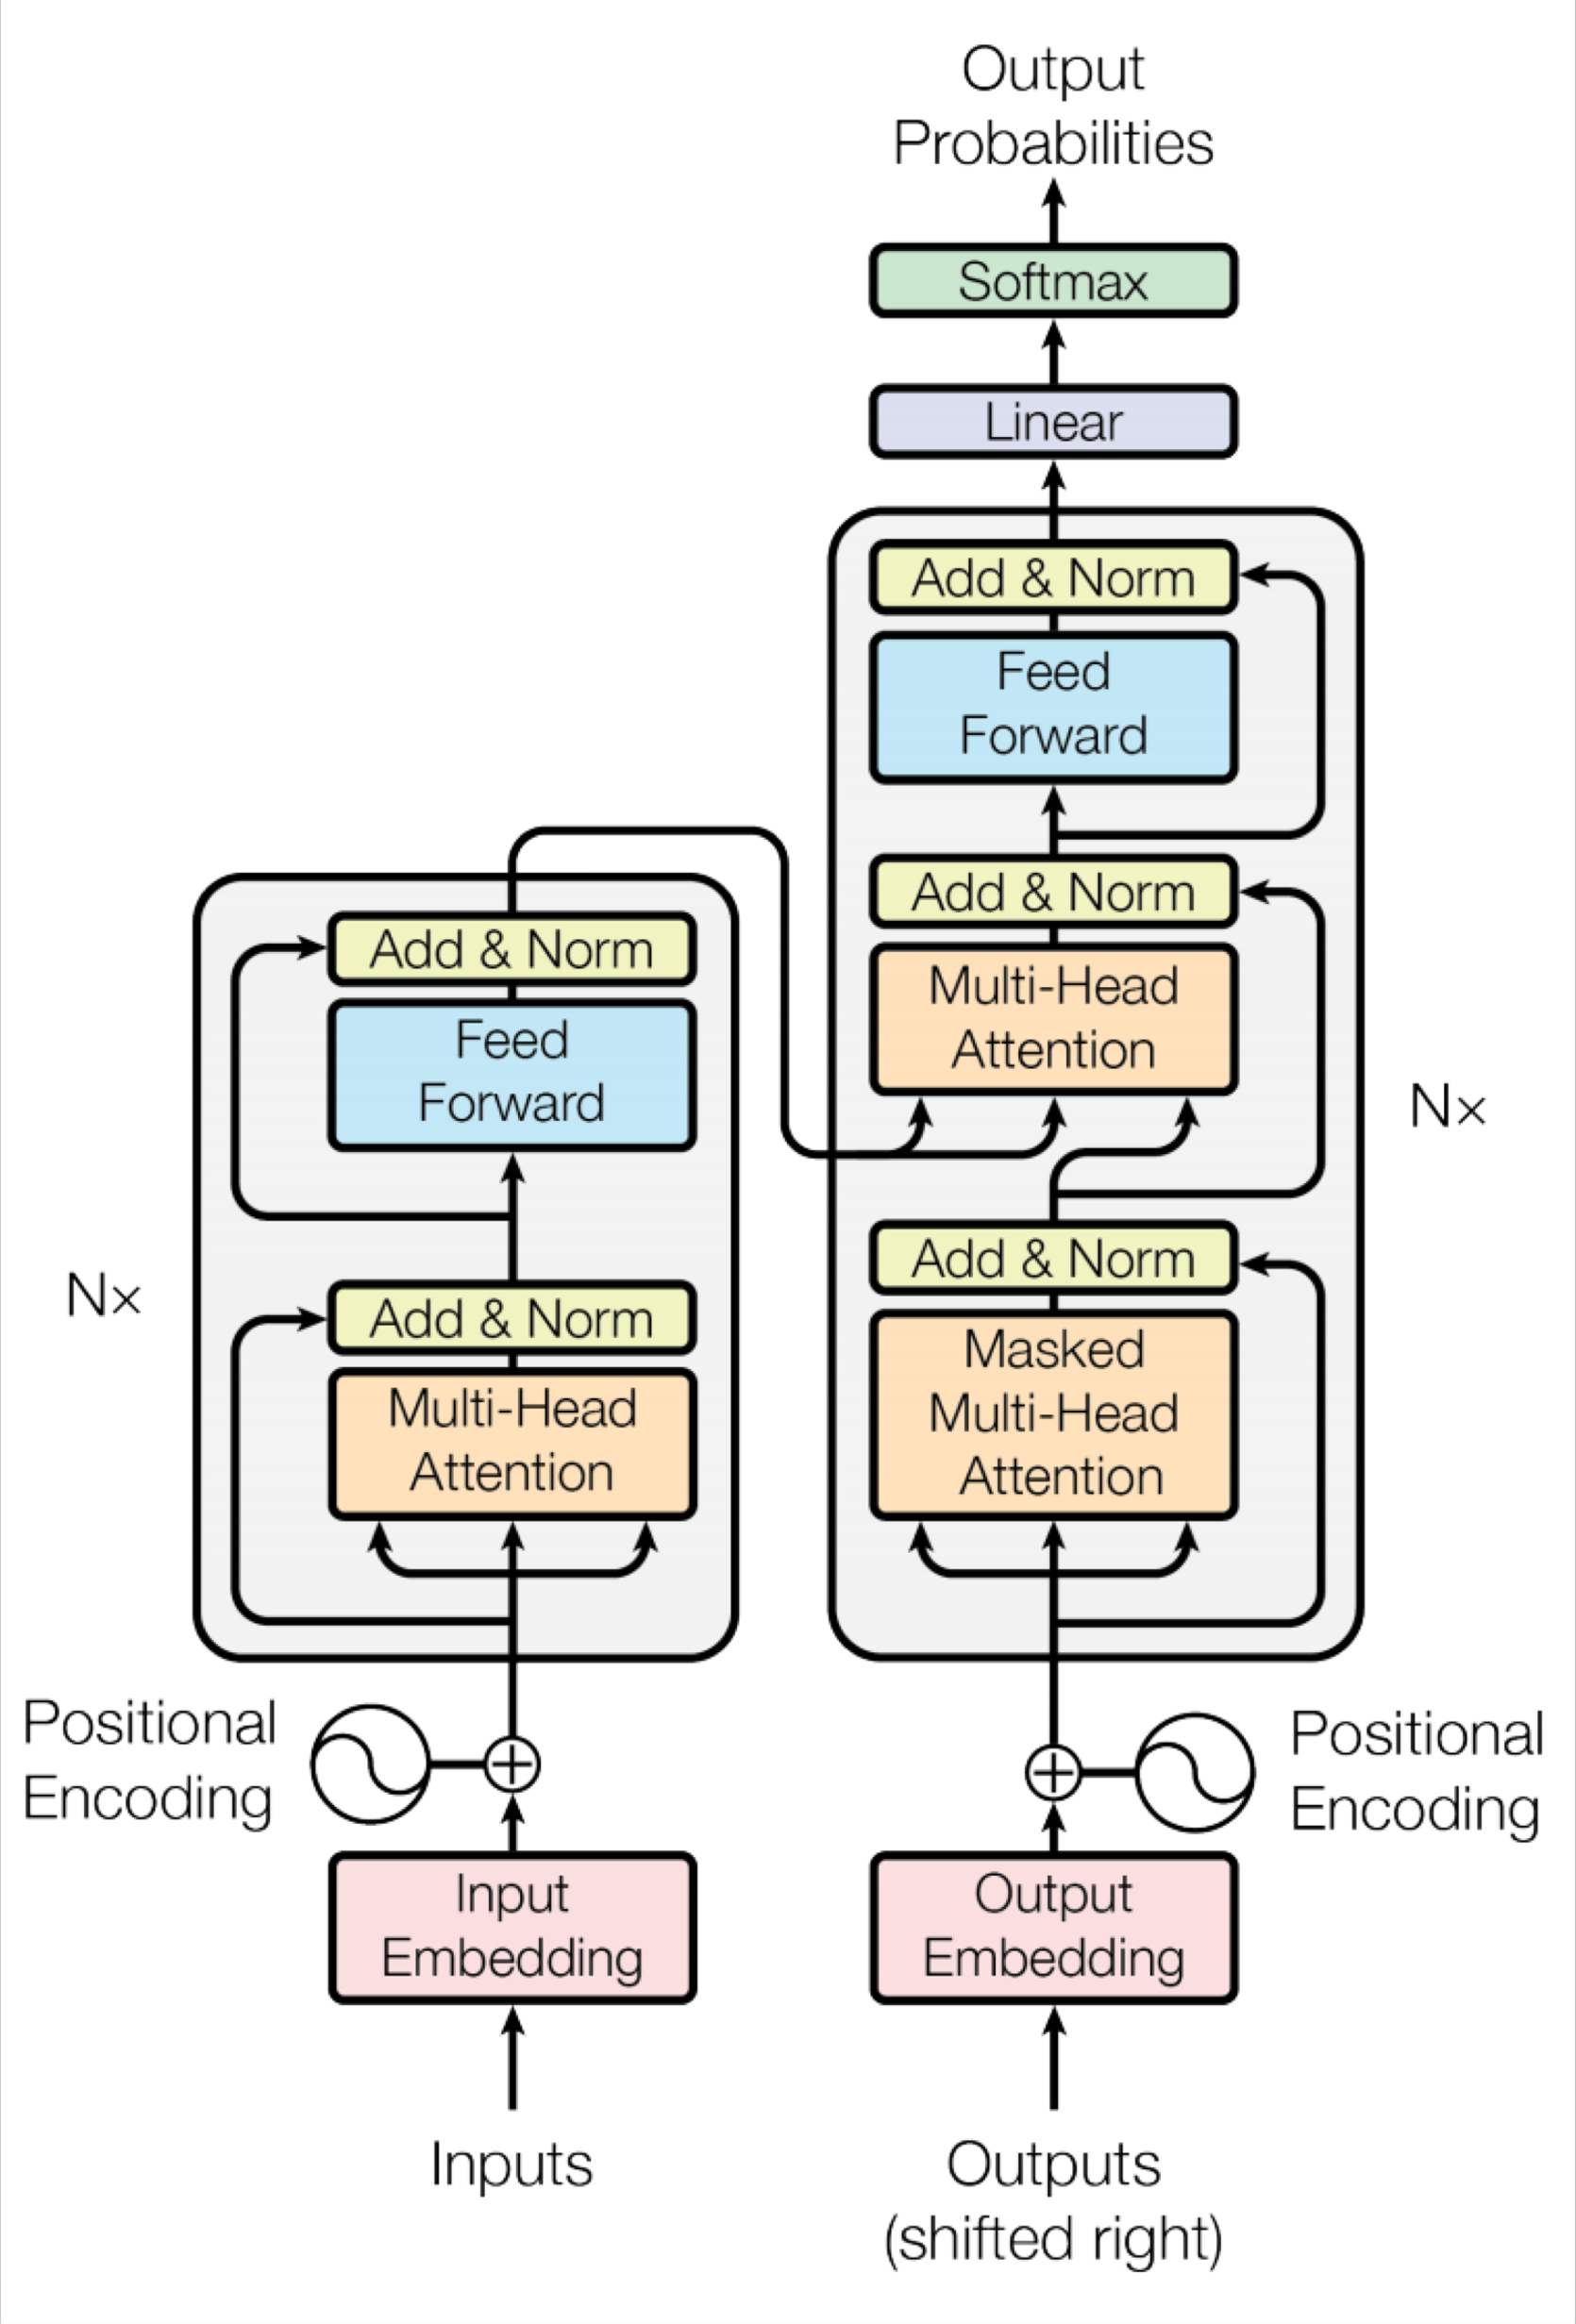
\includegraphics[width=0.8\linewidth,keepaspectratio]{bert69}
			% \end{center}		
		% \end{column}
    % \begin{column}[T]{0.5\linewidth}
		% Attention is all you need. 2017.  Aswani, Shazeer, Parmar, Uszkoreit,  Jones, Gomez, Kaiser, Polosukhin  https://arxiv.org/pdf/1706.03762.pdf 

      % \begin{itemize}
			% \item Non-recurrent sequence-to-  sequence encoder-decoder model
			% \item Task: machine translation  with parallel corpus
			% \item Predict each translated word
			% \item Final cost/error function is  standard cross-entropy error on top of a softmax classifier
			% \end{itemize}
    % \end{column}
  % \end{columns}
			
% \end{frame}

% %%%%%%%%%%%%%%%%%%%%%%%%%%%%%%%%%%%%%%%%%%%%%%%%%%%%%%%%%%%
% \begin{frame}[fragile]\frametitle{Transformer Encoder}

% \begin{columns}
    % \begin{column}[T]{0.5\linewidth}
			% \begin{center}
			% 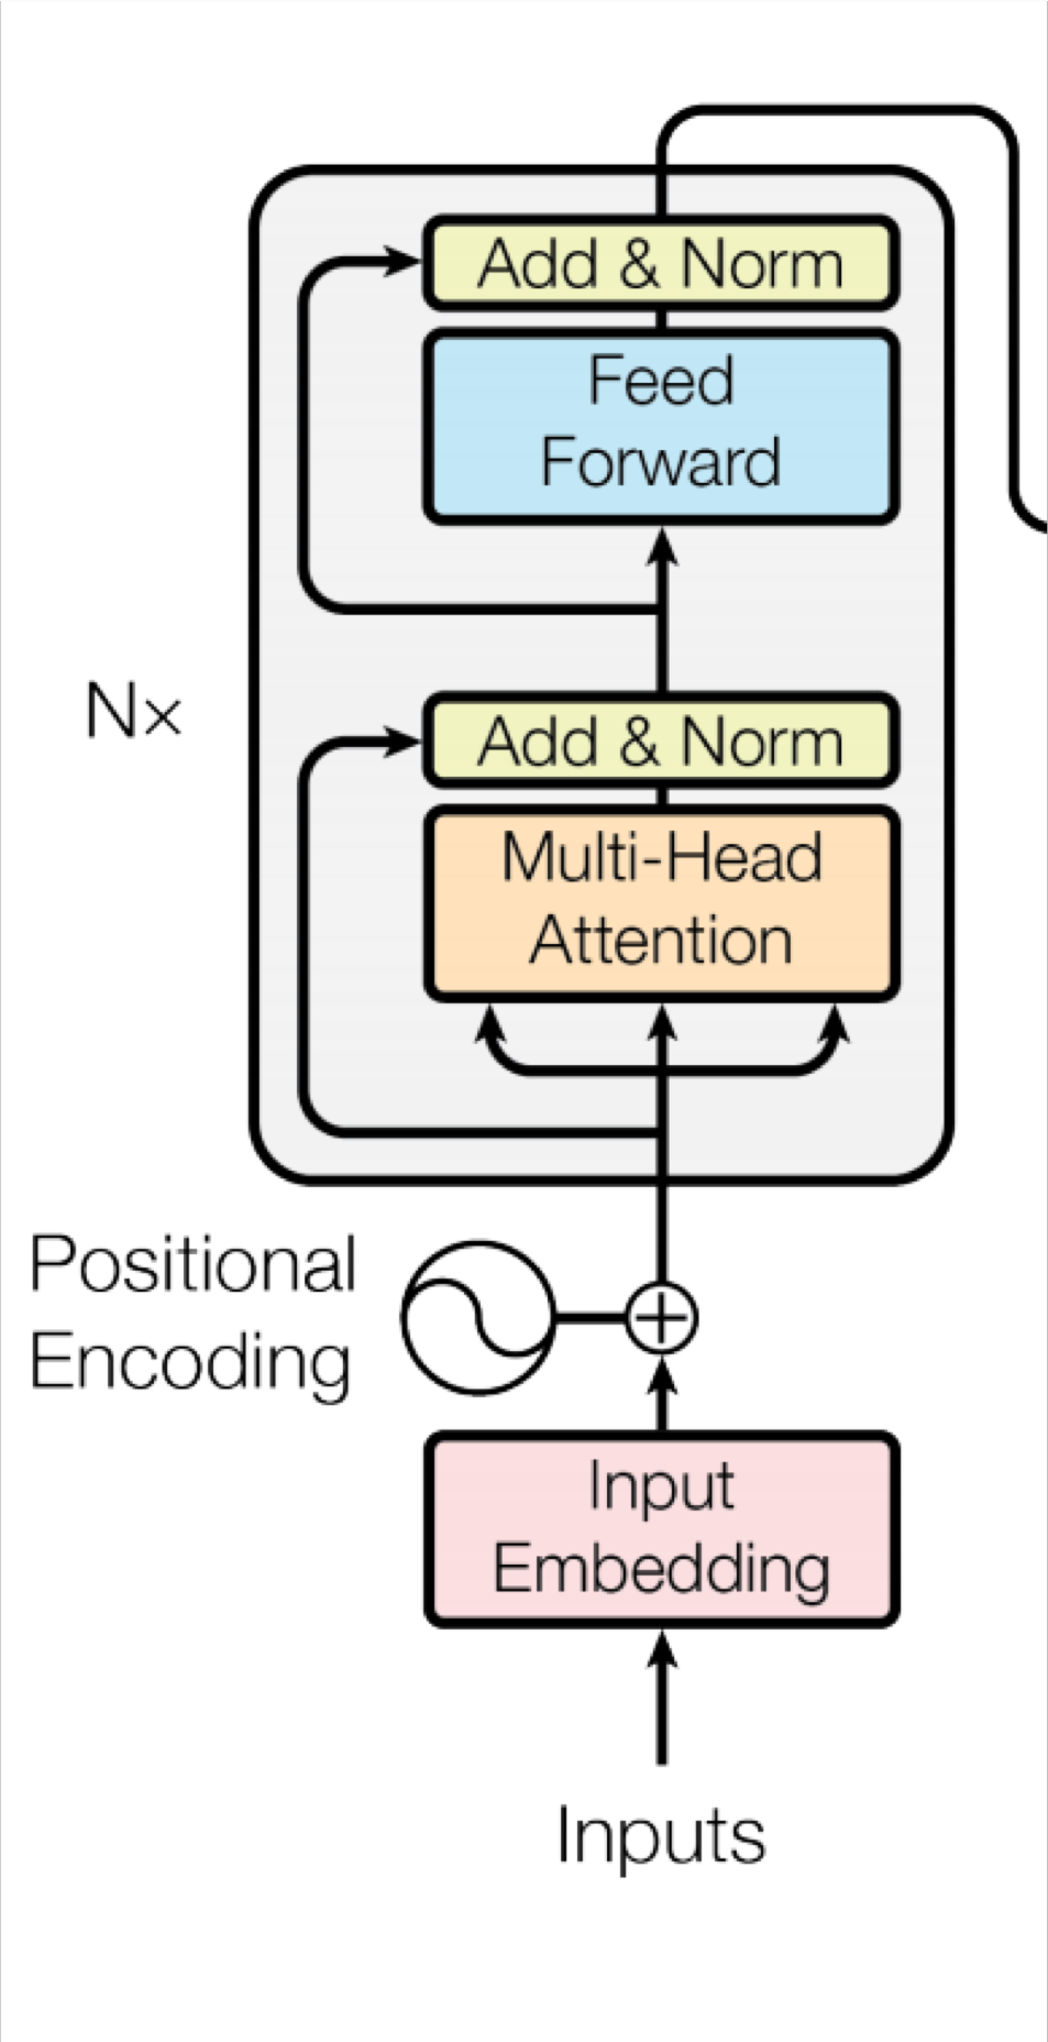
\includegraphics[width=0.6\linewidth,keepaspectratio]{bert70}
			% \end{center}		
		% \end{column}
    % \begin{column}[T]{0.5\linewidth}
      % \begin{itemize}
			% \item For encoder, at each block, we use the same Q, K and V; from the previous layer
			% \item Blocks are repeated 6 times (in vertical stack)
			% \end{itemize}
    % \end{column}
  % \end{columns}
			
% \end{frame}

% %%%%%%%%%%%%%%%%%%%%%%%%%%%%%%%%%%%%%%%%%%%%%%%%%%%%%%%%%%%
% \begin{frame}[fragile]\frametitle{Transformer Decoder}


			% \begin{center}
			% 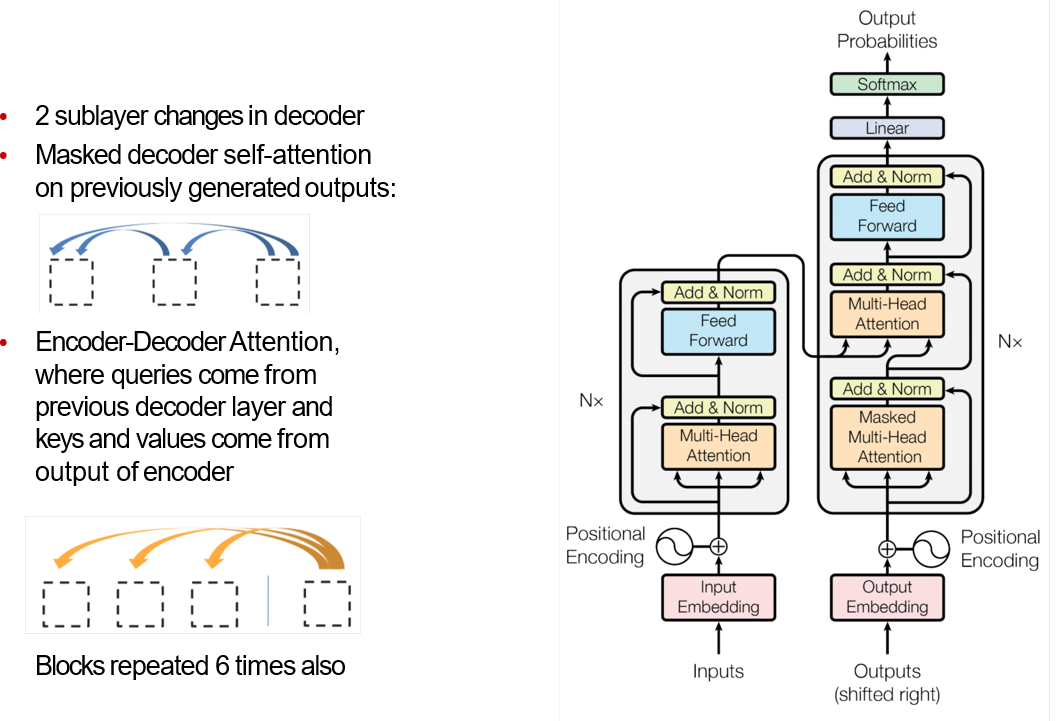
\includegraphics[width=\linewidth,keepaspectratio]{bert71}
			% \end{center}		

			
% \end{frame}

% %%%%%%%%%%%%%%%%%%%%%%%%%%%%%%%%%%%%%%%%%%%%%%%%%%%%%%%%%%%
% \begin{frame}[fragile]\frametitle{Transformer Encoder-Decoder}

			% \begin{center}
			% 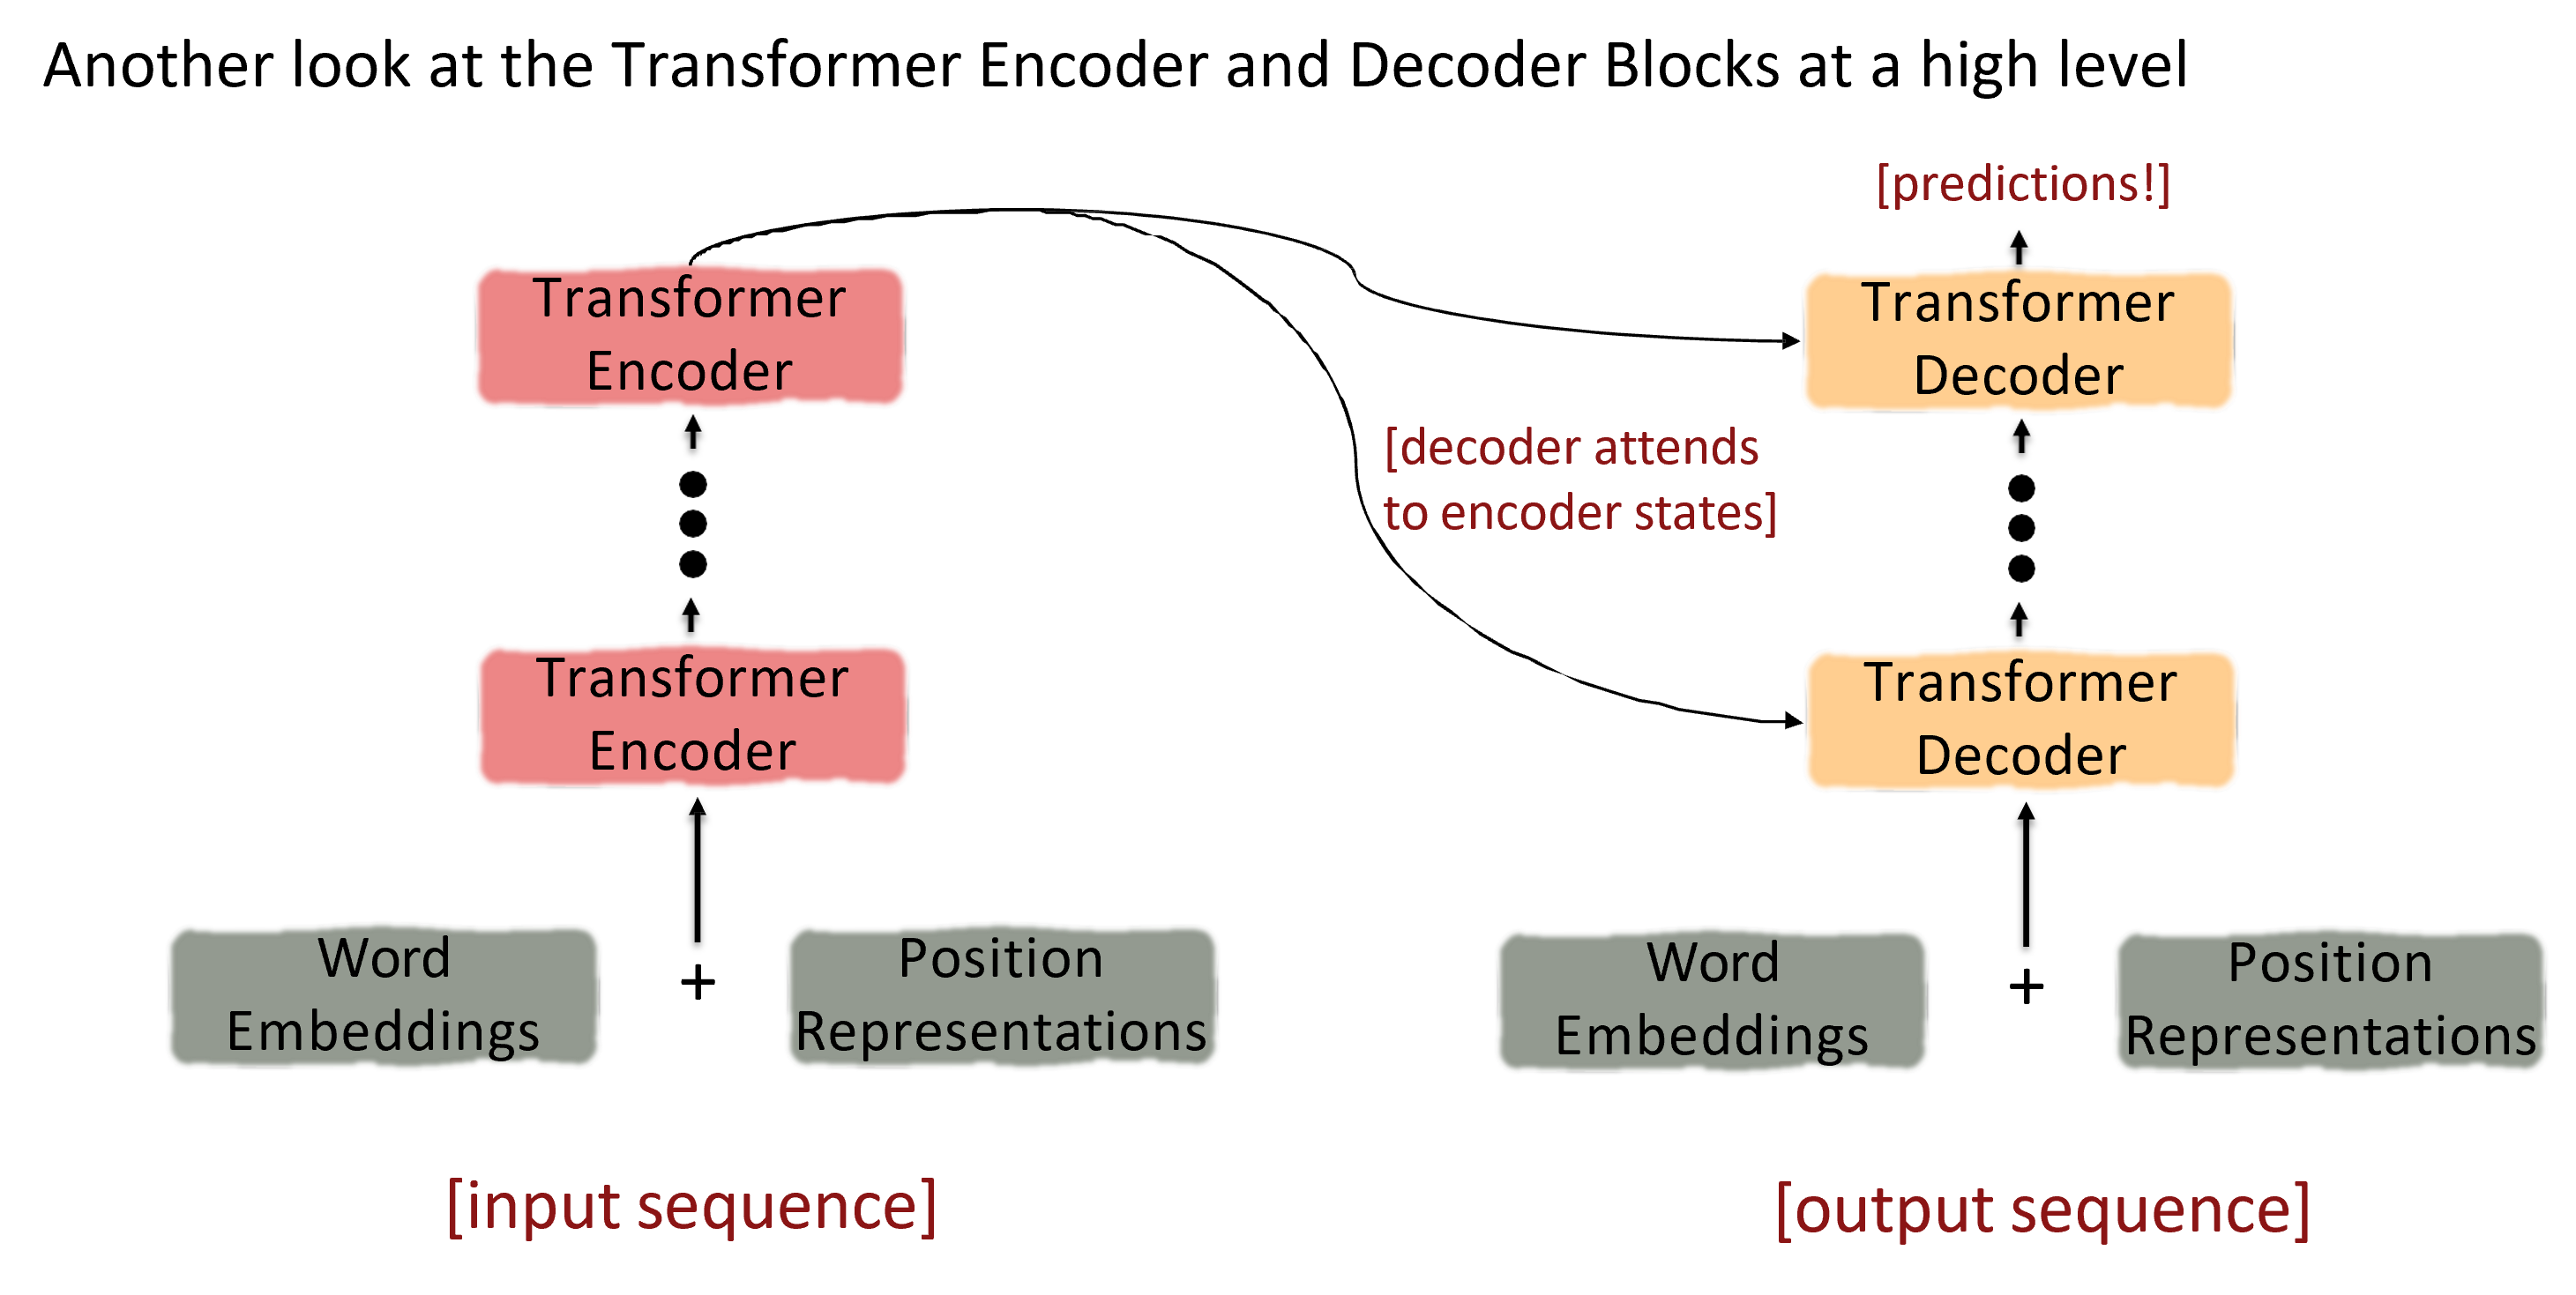
\includegraphics[width=\linewidth,keepaspectratio]{bert72}
			% \end{center}		

			
% \end{frame}

% %%%%%%%%%%%%%%%%%%%%%%%%%%%%%%%%%%%%%%%%%%%%%%%%%%%%%%%%%%%
% \begin{frame}[fragile]\frametitle{Transformer Encoder-Decoder}
% Next, let’s look at the Transformer Encoder and Decoder Blocks

% What’s left in a Transformer Encoder Block that we haven’t covered?

      % \begin{itemize}
			% \item Key-query-value attention: How do we get the $k,q,v$ vectors from a single word embedding?
			% \item Multi-headed attention: Attend to multiple places in a single layer!
			% \item Tricks to help with training!
			    % \begin{itemize}
					% \item Residual connections
					% \item Layer normalization
					% \item Scaling the dot product
					% \item These tricks don’t improve what the model is able to do; they help improve the training process
					% \end{itemize}

			% \end{itemize}
			
% \end{frame}

% %%%%%%%%%%%%%%%%%%%%%%%%%%%%%%%%%%%%%%%%%%%%%%%%%%%%%%%%%%%
% \begin{frame}[fragile]\frametitle{The Transformer Encoder: Dot-Product Attention}


      % \begin{itemize}
			% \item Inputs: a query q and a set of key-value (k-v) pairs to an output
			% \item Query, keys, values, and output are all vectors
			% \item Output is weighted sum of values, where
			% \item Weight of each value is computed by an inner product of query and corresponding key
			% \item Queries and keys have same dimensionality $d_k$ , value have $d_v$
			% \end{itemize}
			
			% \begin{center}
			% 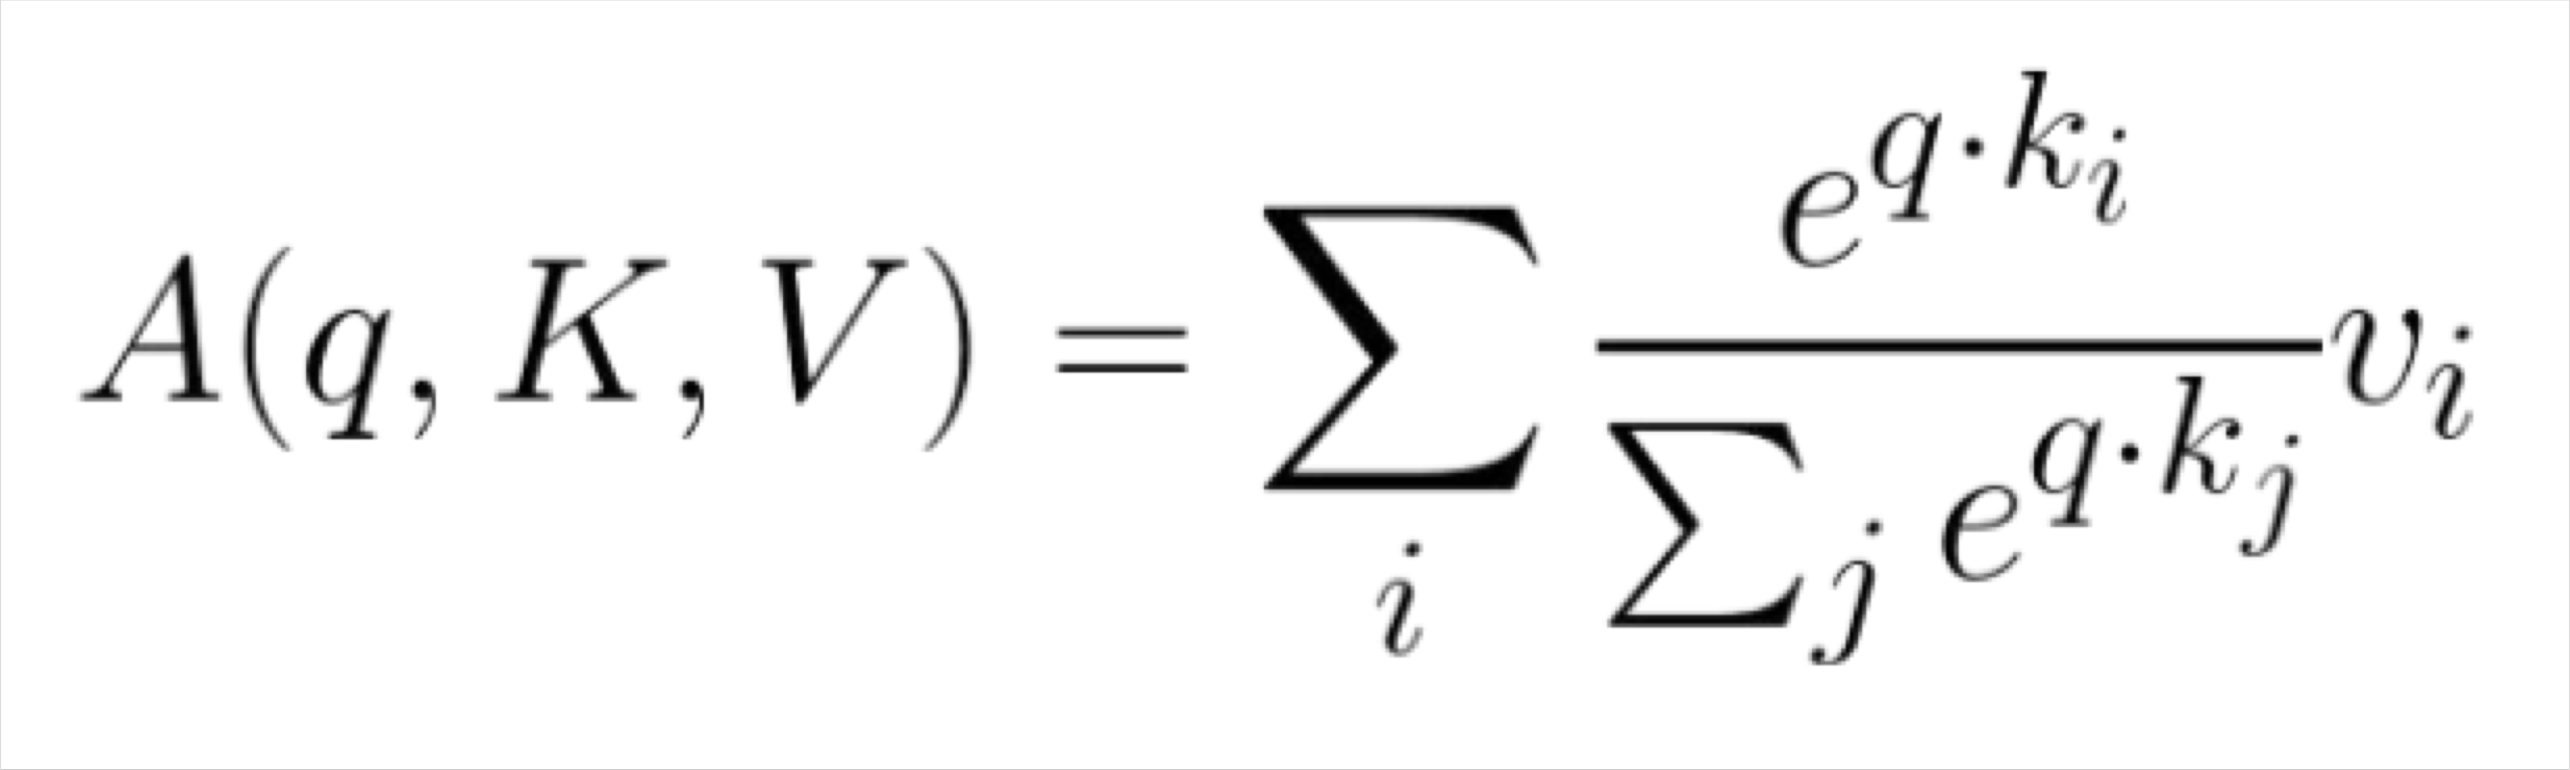
\includegraphics[width=0.4\linewidth,keepaspectratio]{bert73}
			% \end{center}		
			
			% % {\tiny (Ref: CS224n: Natural Language Processing with Deep Learning - Christopher Manning)}

% \end{frame}

% %%%%%%%%%%%%%%%%%%%%%%%%%%%%%%%%%%%%%%%%%%%%%%%%%%%%%%%%%%%
% \begin{frame}[fragile]\frametitle{The Transformer Encoder: Dot-Product Attention: Matrix notation}


      % \begin{itemize}
			% \item Inputs: a query q and a set of key-value (k-v) pairs to an output
			% \item Query, keys, values, and output are all vectors
			% \item Output is weighted sum of values, where
			% \item Weight of each value is computed by an inner product of query and corresponding key
			% \item Queries and keys have same dimensionality $d_k$ , value have $d_v$
			% \end{itemize}
			
			% \begin{center}
			% 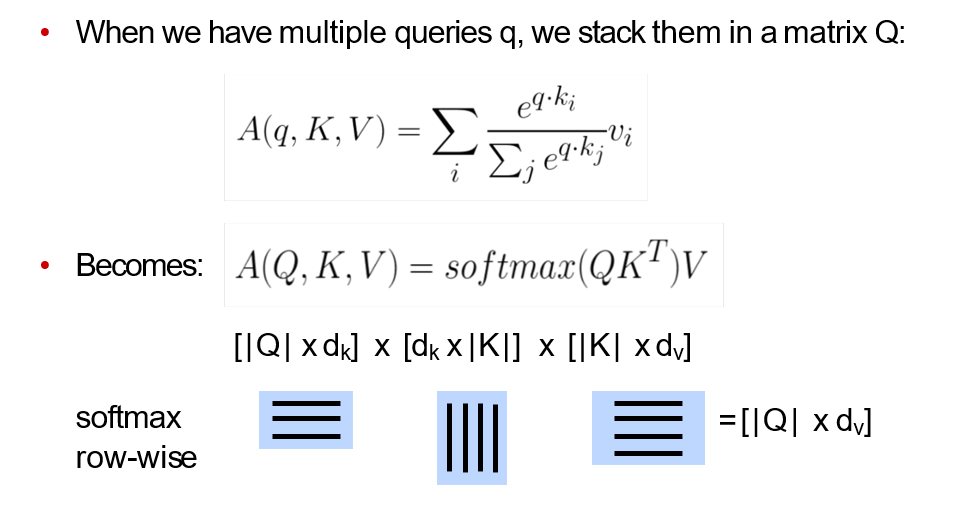
\includegraphics[width=0.8\linewidth,keepaspectratio]{bert74}
			% \end{center}		
			
			% % {\tiny (Ref: CS224n: Natural Language Processing with Deep Learning - Christopher Manning)}

% \end{frame}

% %%%%%%%%%%%%%%%%%%%%%%%%%%%%%%%%%%%%%%%%%%%%%%%%%%%%%%%%%%%
% \begin{frame}[fragile]\frametitle{The Transformer Encoder: Key-Query-Value Attention}

			
			% \begin{center}
			% 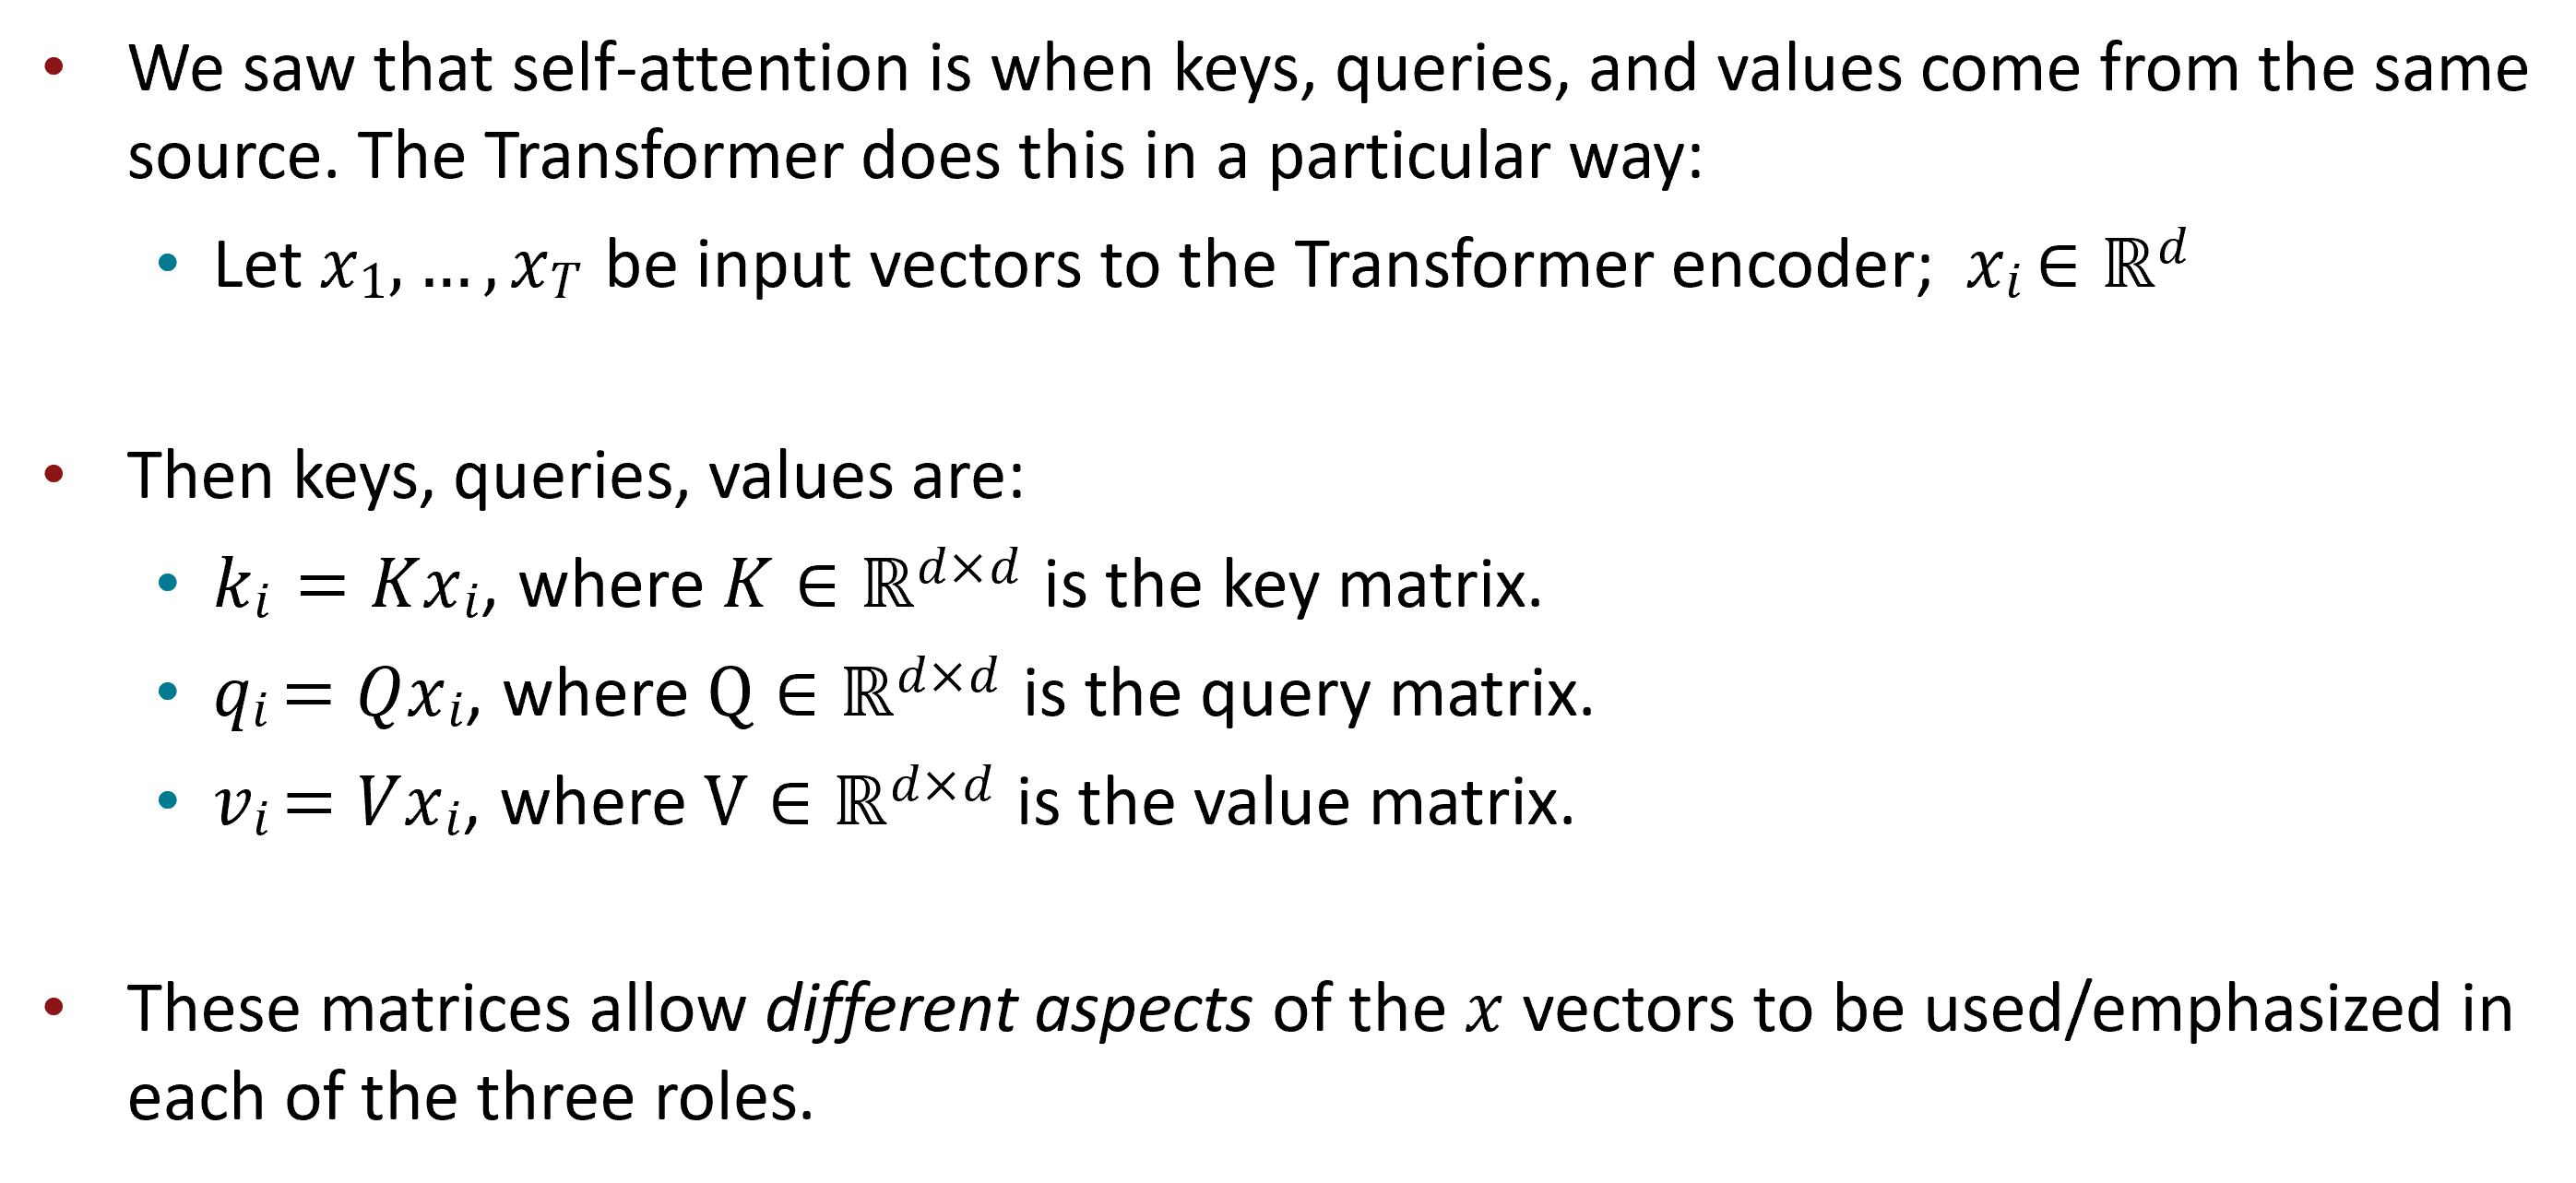
\includegraphics[width=\linewidth,keepaspectratio]{bert75}
			% \end{center}		
			
% % {\tiny (Ref: Language \& Machine Learning - John Hewitt)}

% \end{frame}

% %%%%%%%%%%%%%%%%%%%%%%%%%%%%%%%%%%%%%%%%%%%%%%%%%%%%%%%%%%%
% \begin{frame}[fragile]\frametitle{The Transformer Encoder: Key-Query-Value Attention}

			
			% \begin{center}
			% 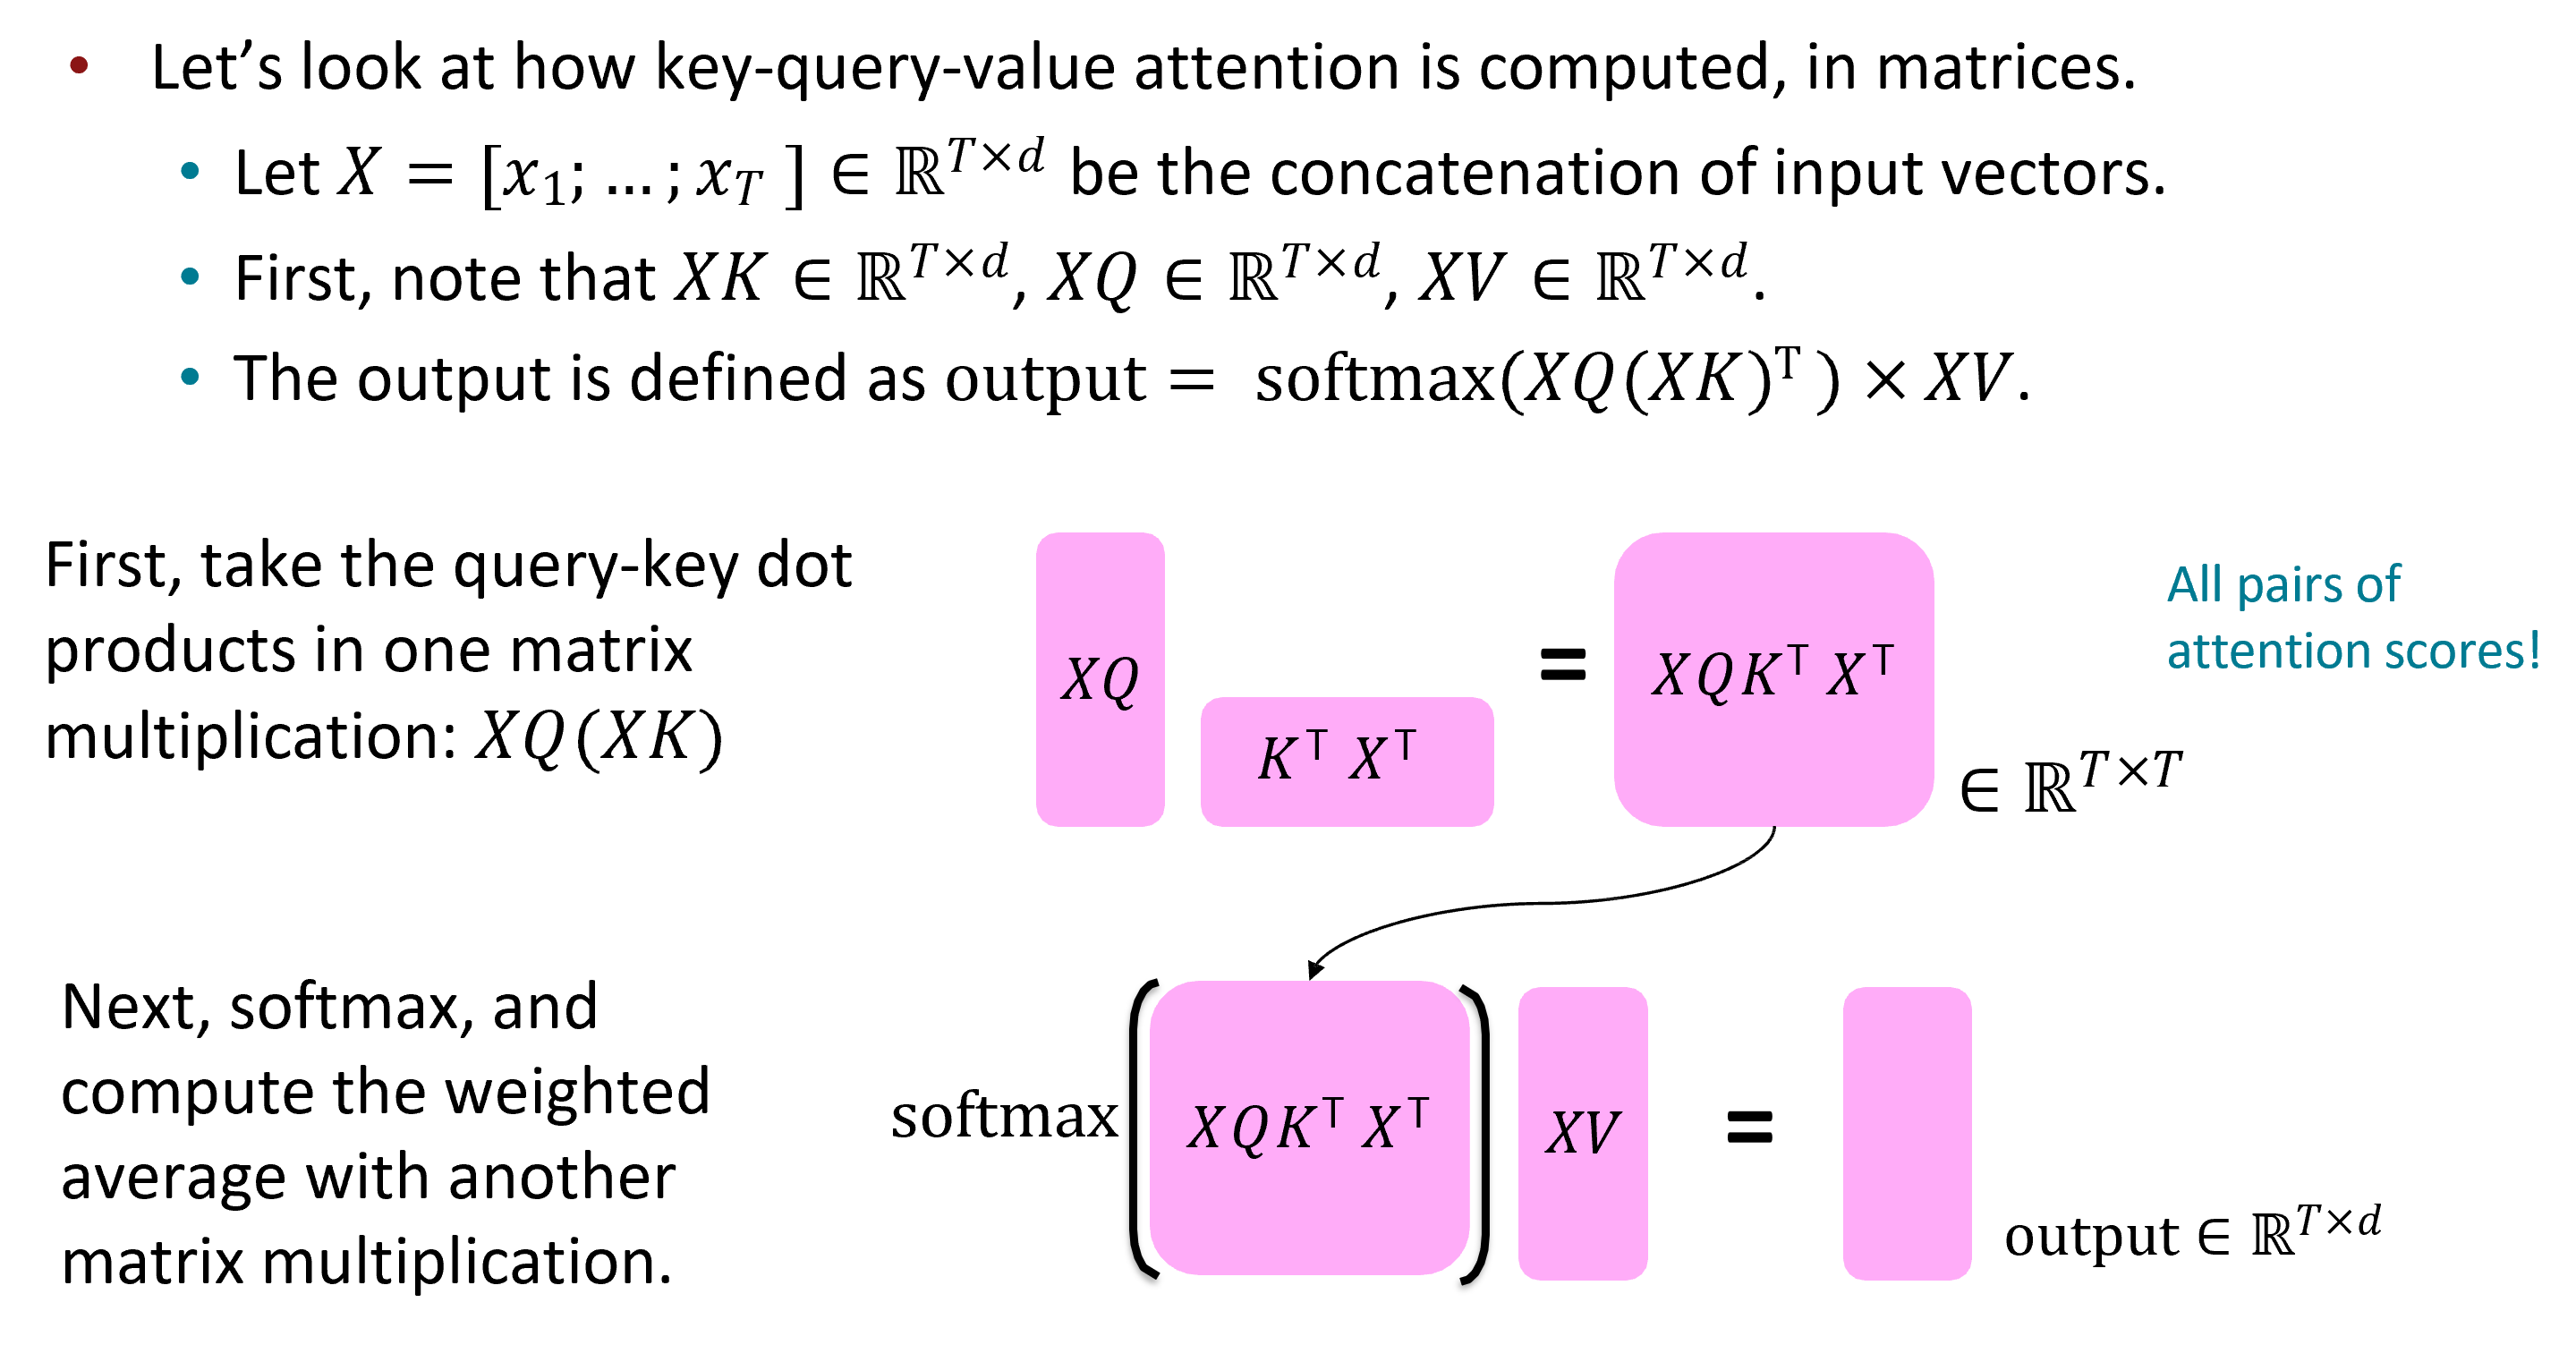
\includegraphics[width=\linewidth,keepaspectratio]{bert76}
			% \end{center}		
			
% % {\tiny (Ref: Language \& Machine Learning - John Hewitt)}

% \end{frame}

% %%%%%%%%%%%%%%%%%%%%%%%%%%%%%%%%%%%%%%%%%%%%%%%%%%%%%%%%%%%
% \begin{frame}[fragile]\frametitle{The Transformer Encoder: Multi-headed attention}

			
			% \begin{center}
			% 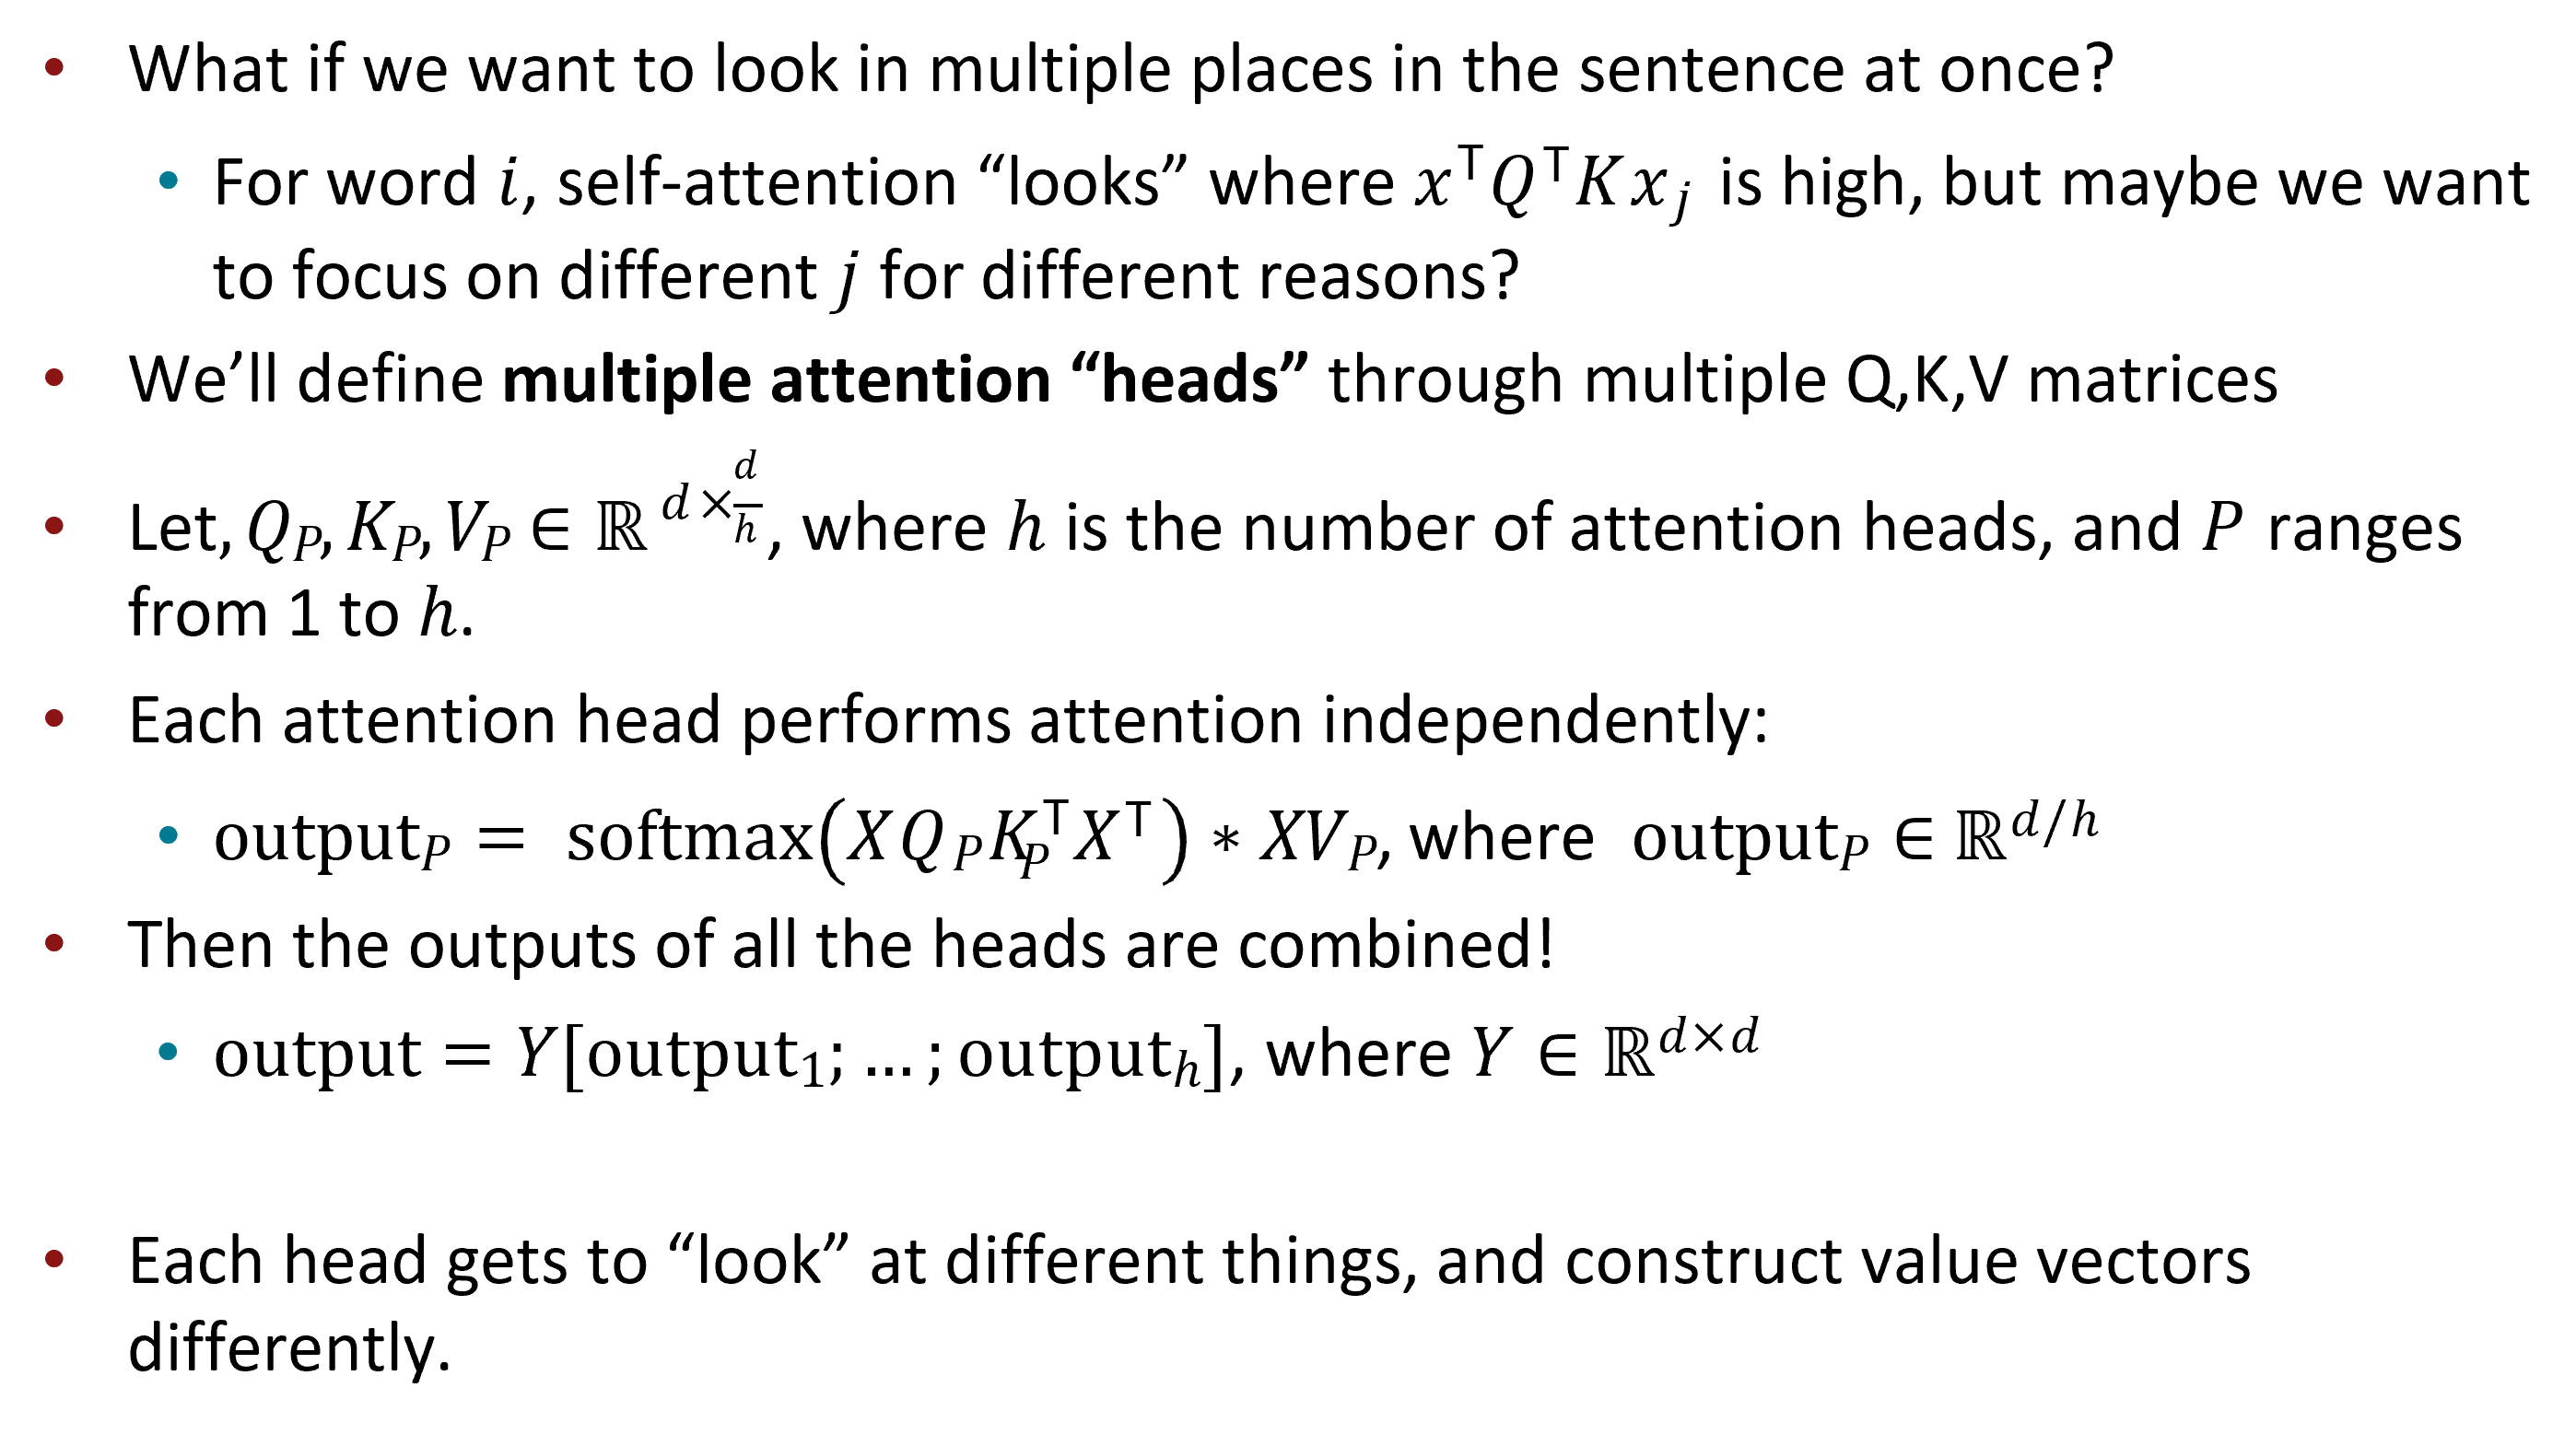
\includegraphics[width=\linewidth,keepaspectratio]{bert77}
			% \end{center}		
			
% % {\tiny (Ref: Language \& Machine Learning - John Hewitt)}

% \end{frame}

% %%%%%%%%%%%%%%%%%%%%%%%%%%%%%%%%%%%%%%%%%%%%%%%%%%%%%%%%%%%
% \begin{frame}[fragile]\frametitle{The Transformer Encoder: Multi-headed attention}

			
			% \begin{center}
			% 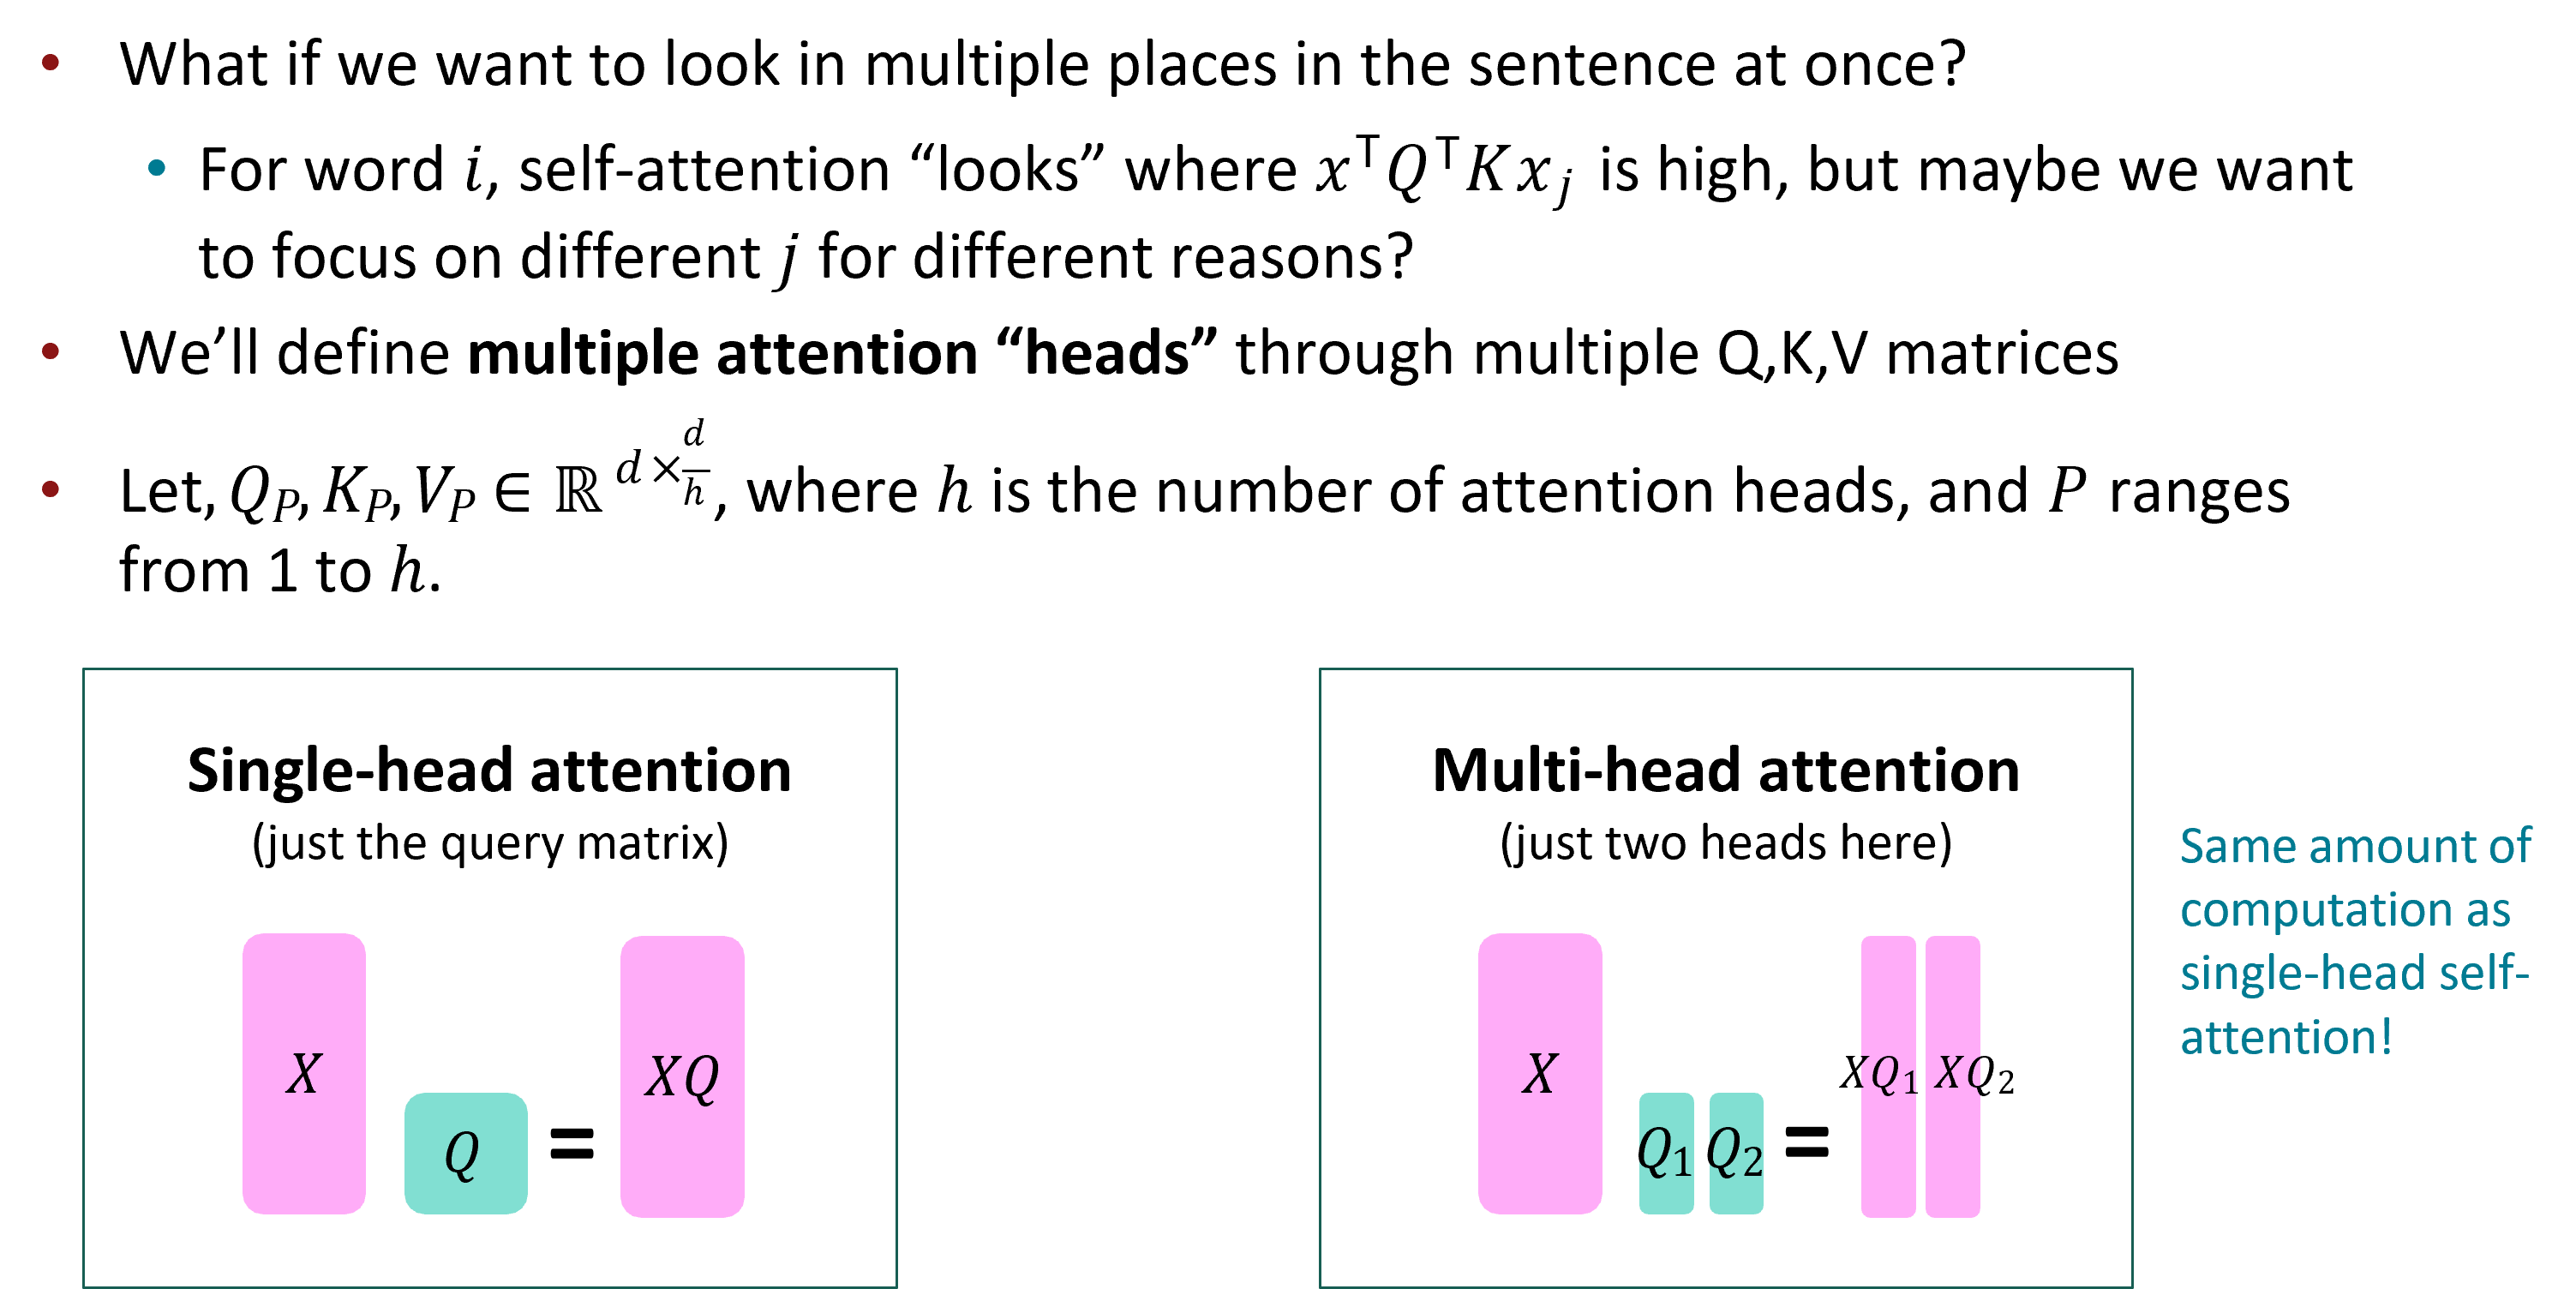
\includegraphics[width=\linewidth,keepaspectratio]{bert78}
			% \end{center}		
			
% % {\tiny (Ref: Language \& Machine Learning - John Hewitt)}

% \end{frame}

% %%%%%%%%%%%%%%%%%%%%%%%%%%%%%%%%%%%%%%%%%%%%%%%%%%%%%%%%%%%
% \begin{frame}[fragile]\frametitle{Attention visualization in layer 5}

			
			% \begin{center}
			% 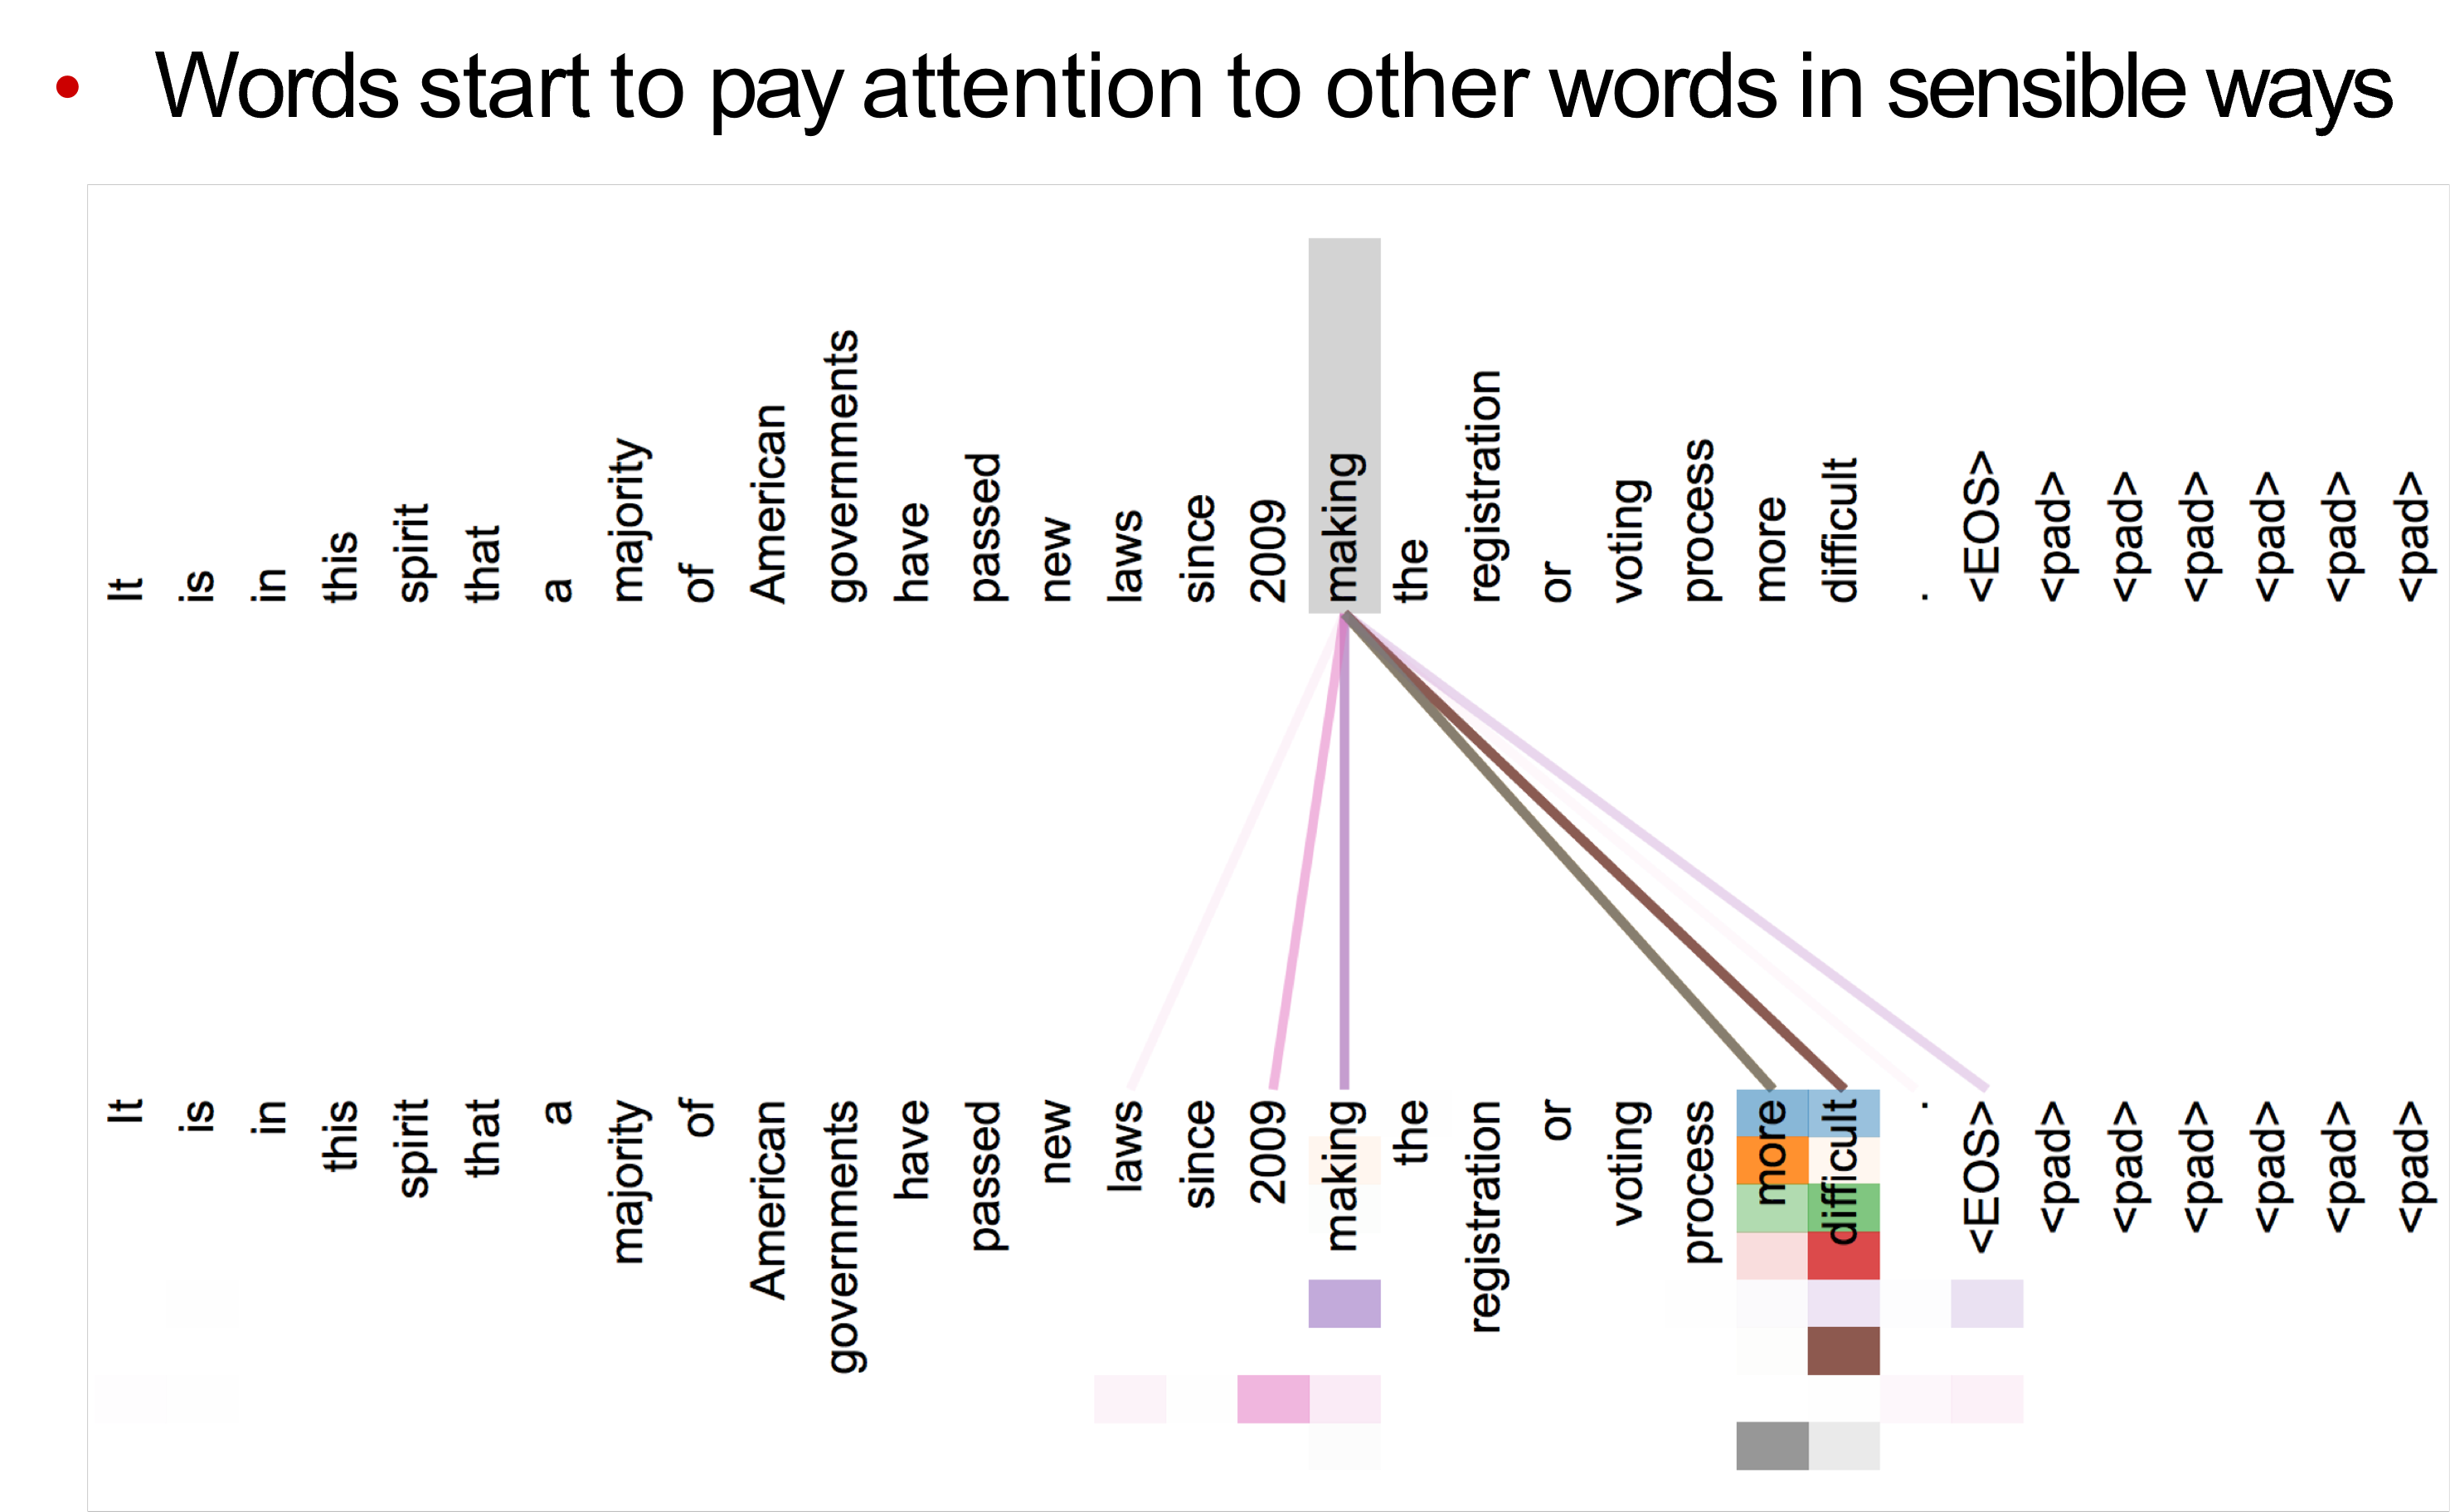
\includegraphics[width=0.8\linewidth,keepaspectratio]{bert79}
			% \end{center}		
			
			% % {\tiny (Ref: CS224n: Natural Language Processing with Deep Learning - Christopher Manning)}

% \end{frame}

% %%%%%%%%%%%%%%%%%%%%%%%%%%%%%%%%%%%%%%%%%%%%%%%%%%%%%%%%%%%
% \begin{frame}[fragile]\frametitle{Attention visualization: Implicit anaphora resolution}

			
			% \begin{center}
			% 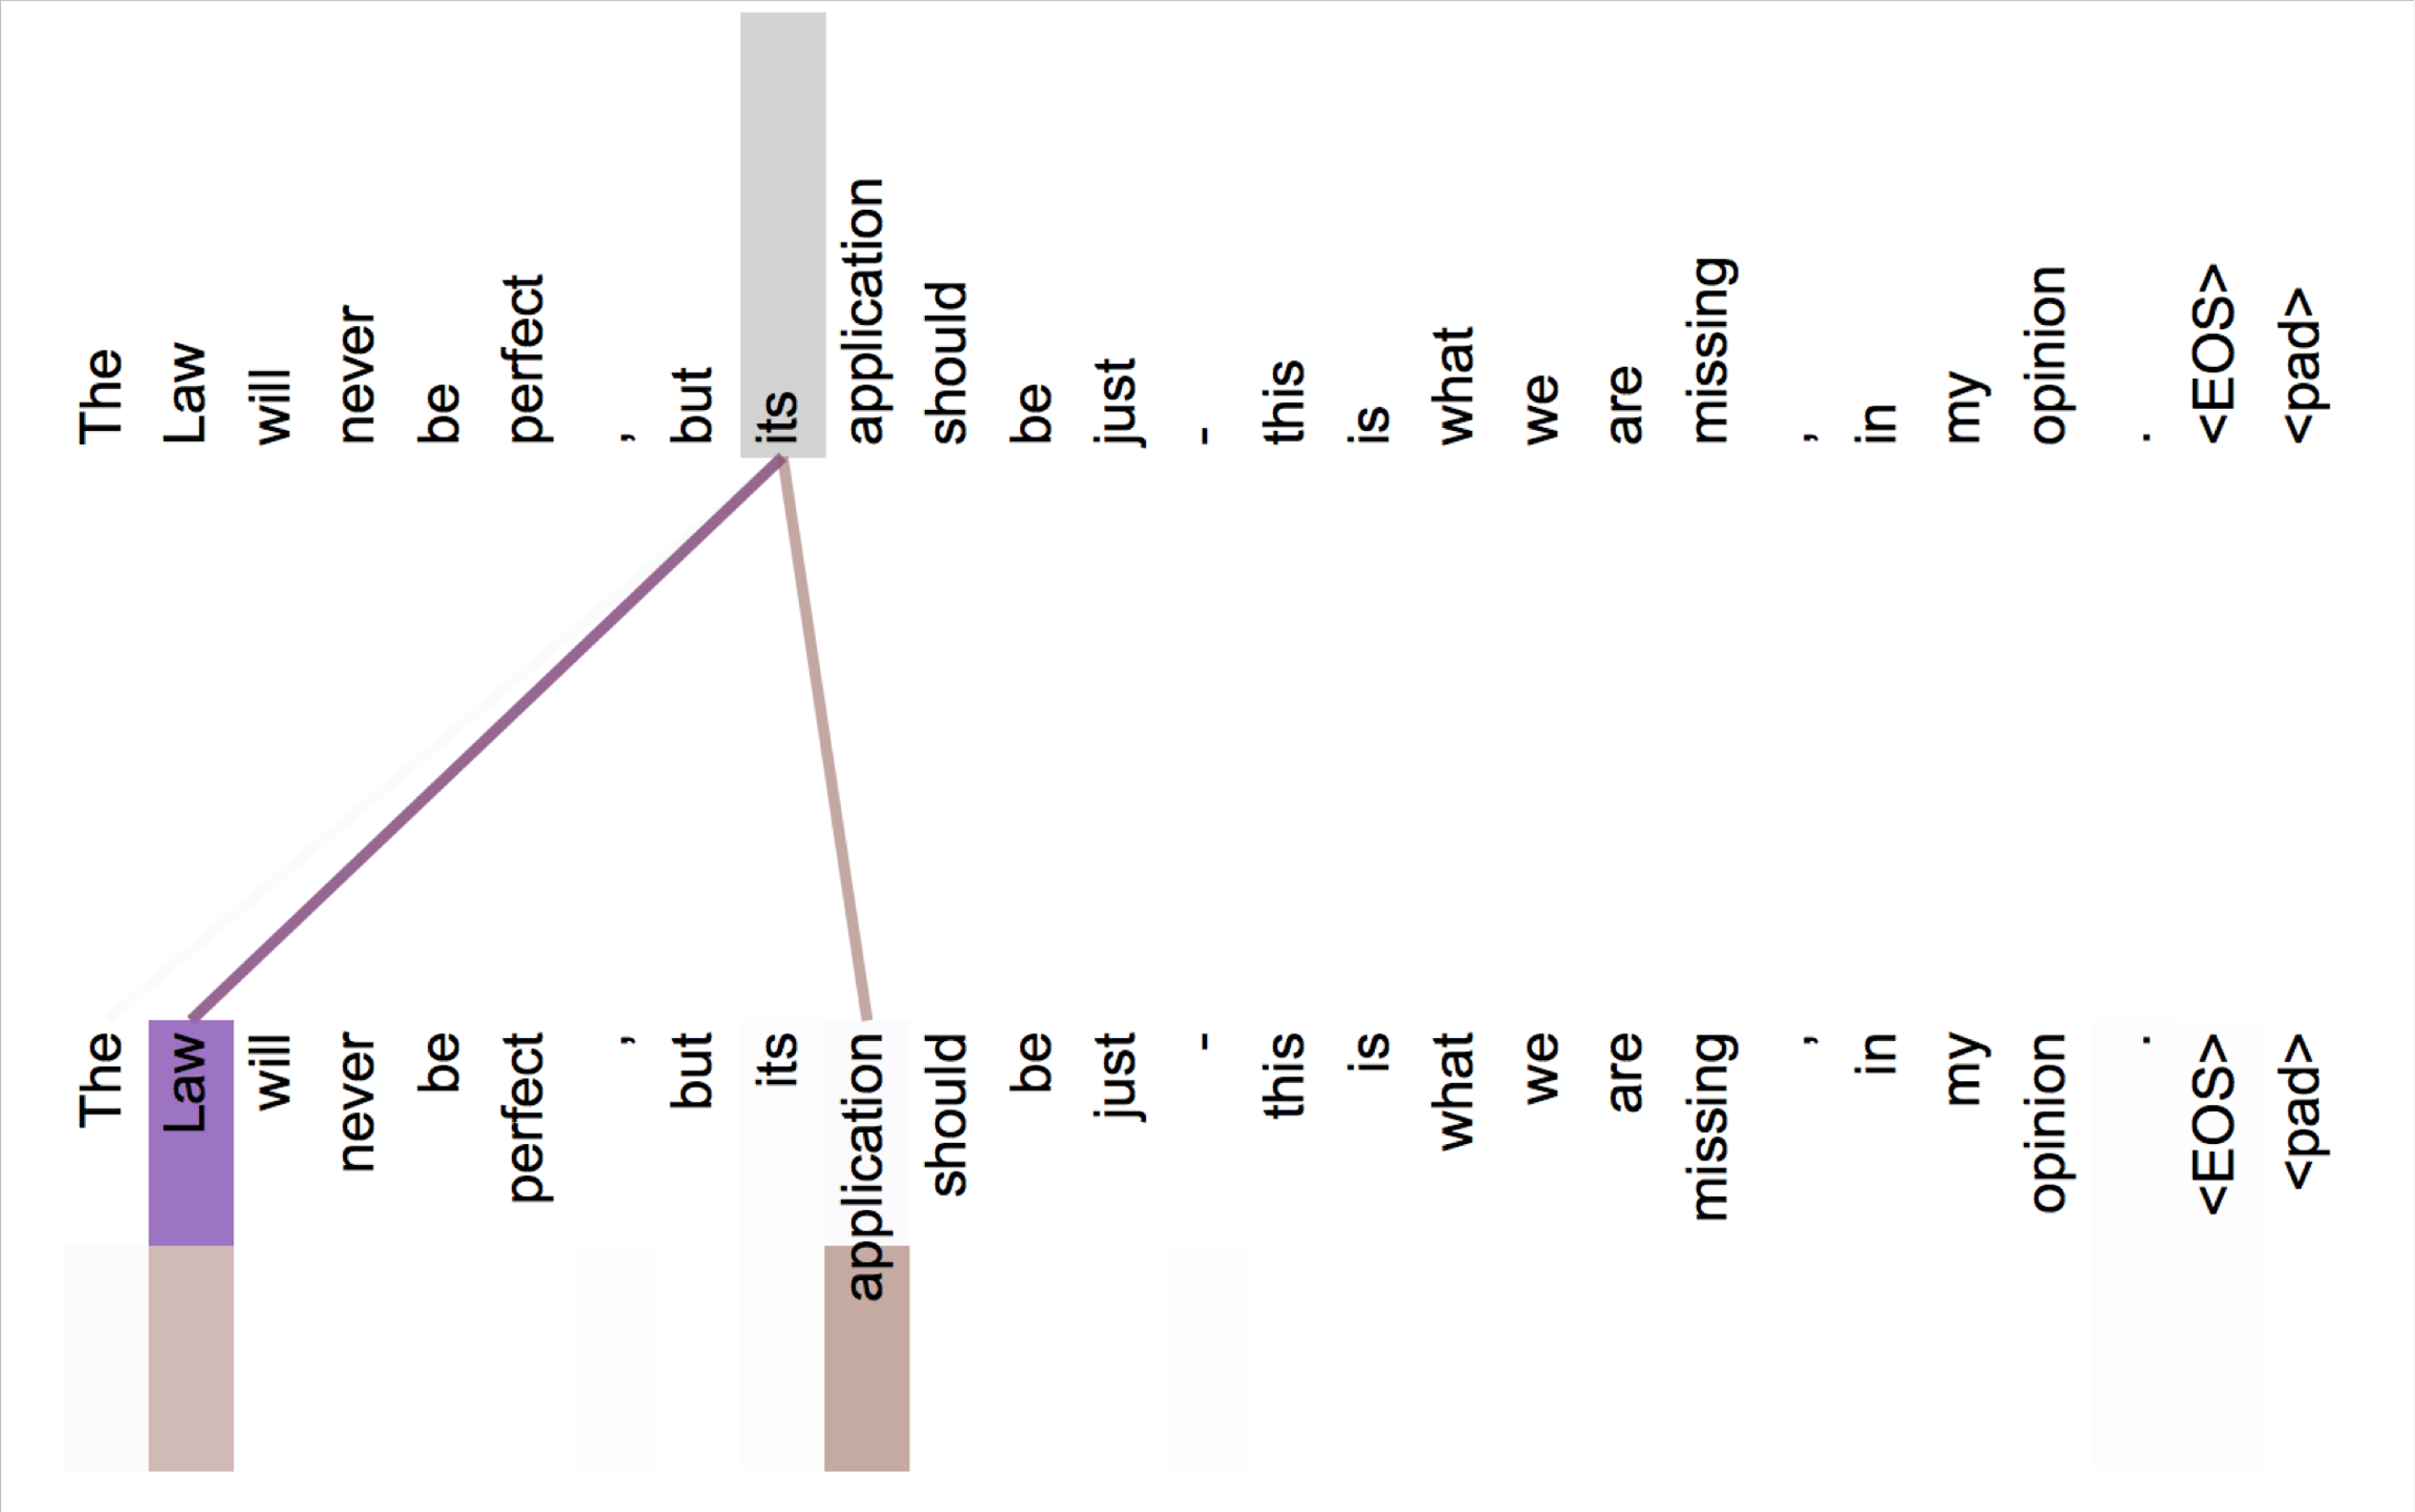
\includegraphics[width=0.6\linewidth,keepaspectratio]{bert80}
			% \end{center}		
			
			% In 5th layer. Isolated attentions from just the word ‘its’ for attention heads 5 and 6.  Note that the attentions are very sharp for this word.

			
			% % {\tiny (Ref: CS224n: Natural Language Processing with Deep Learning - Christopher Manning)}

% \end{frame}

% %%%%%%%%%%%%%%%%%%%%%%%%%%%%%%%%%%%%%%%%%%%%%%%%%%%%%%%%%%%
% \begin{frame}[fragile]\frametitle{Parallel attention heads}

			
			% \begin{center}
			% 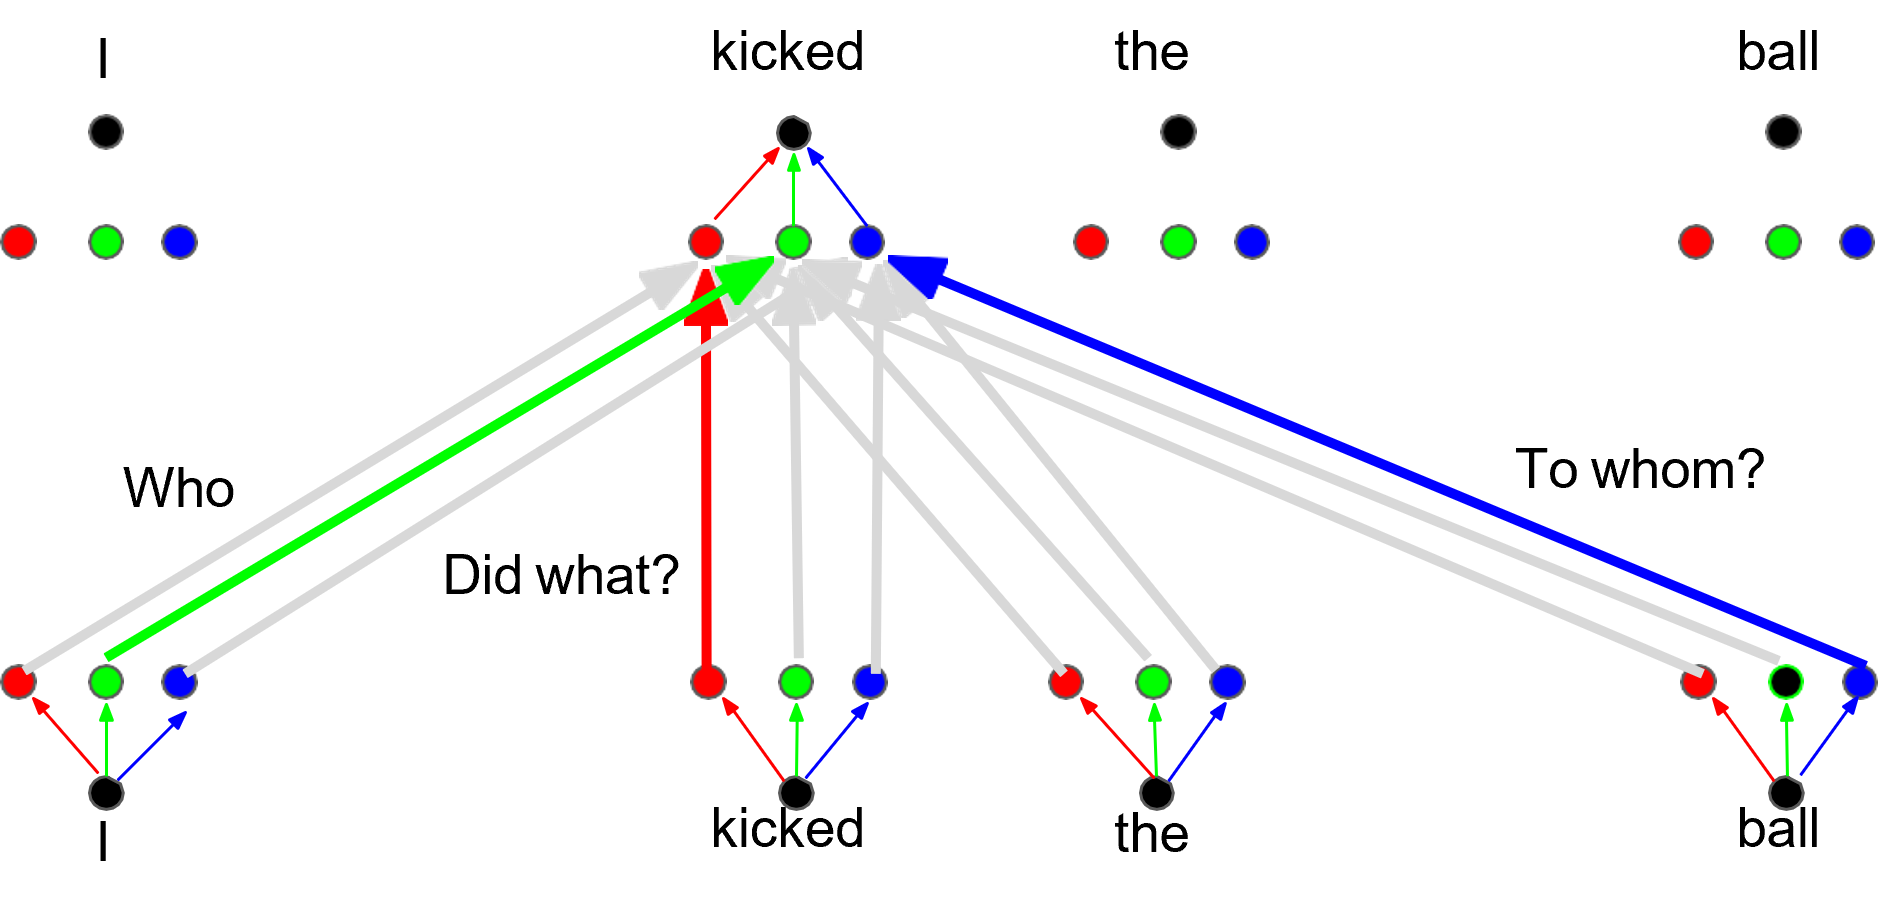
\includegraphics[width=0.6\linewidth,keepaspectratio]{bert81}
			% \end{center}		
			
		
			% % {\tiny (Ref: Ashish Vaswani)}

% \end{frame}

% %%%%%%%%%%%%%%%%%%%%%%%%%%%%%%%%%%%%%%%%%%%%%%%%%%%%%%%%%%%
% \begin{frame}[fragile]\frametitle{Residual connections}

			% The Transformer Encoder: Residual connections [He et al., 2016]
			
			% \begin{center}
			% 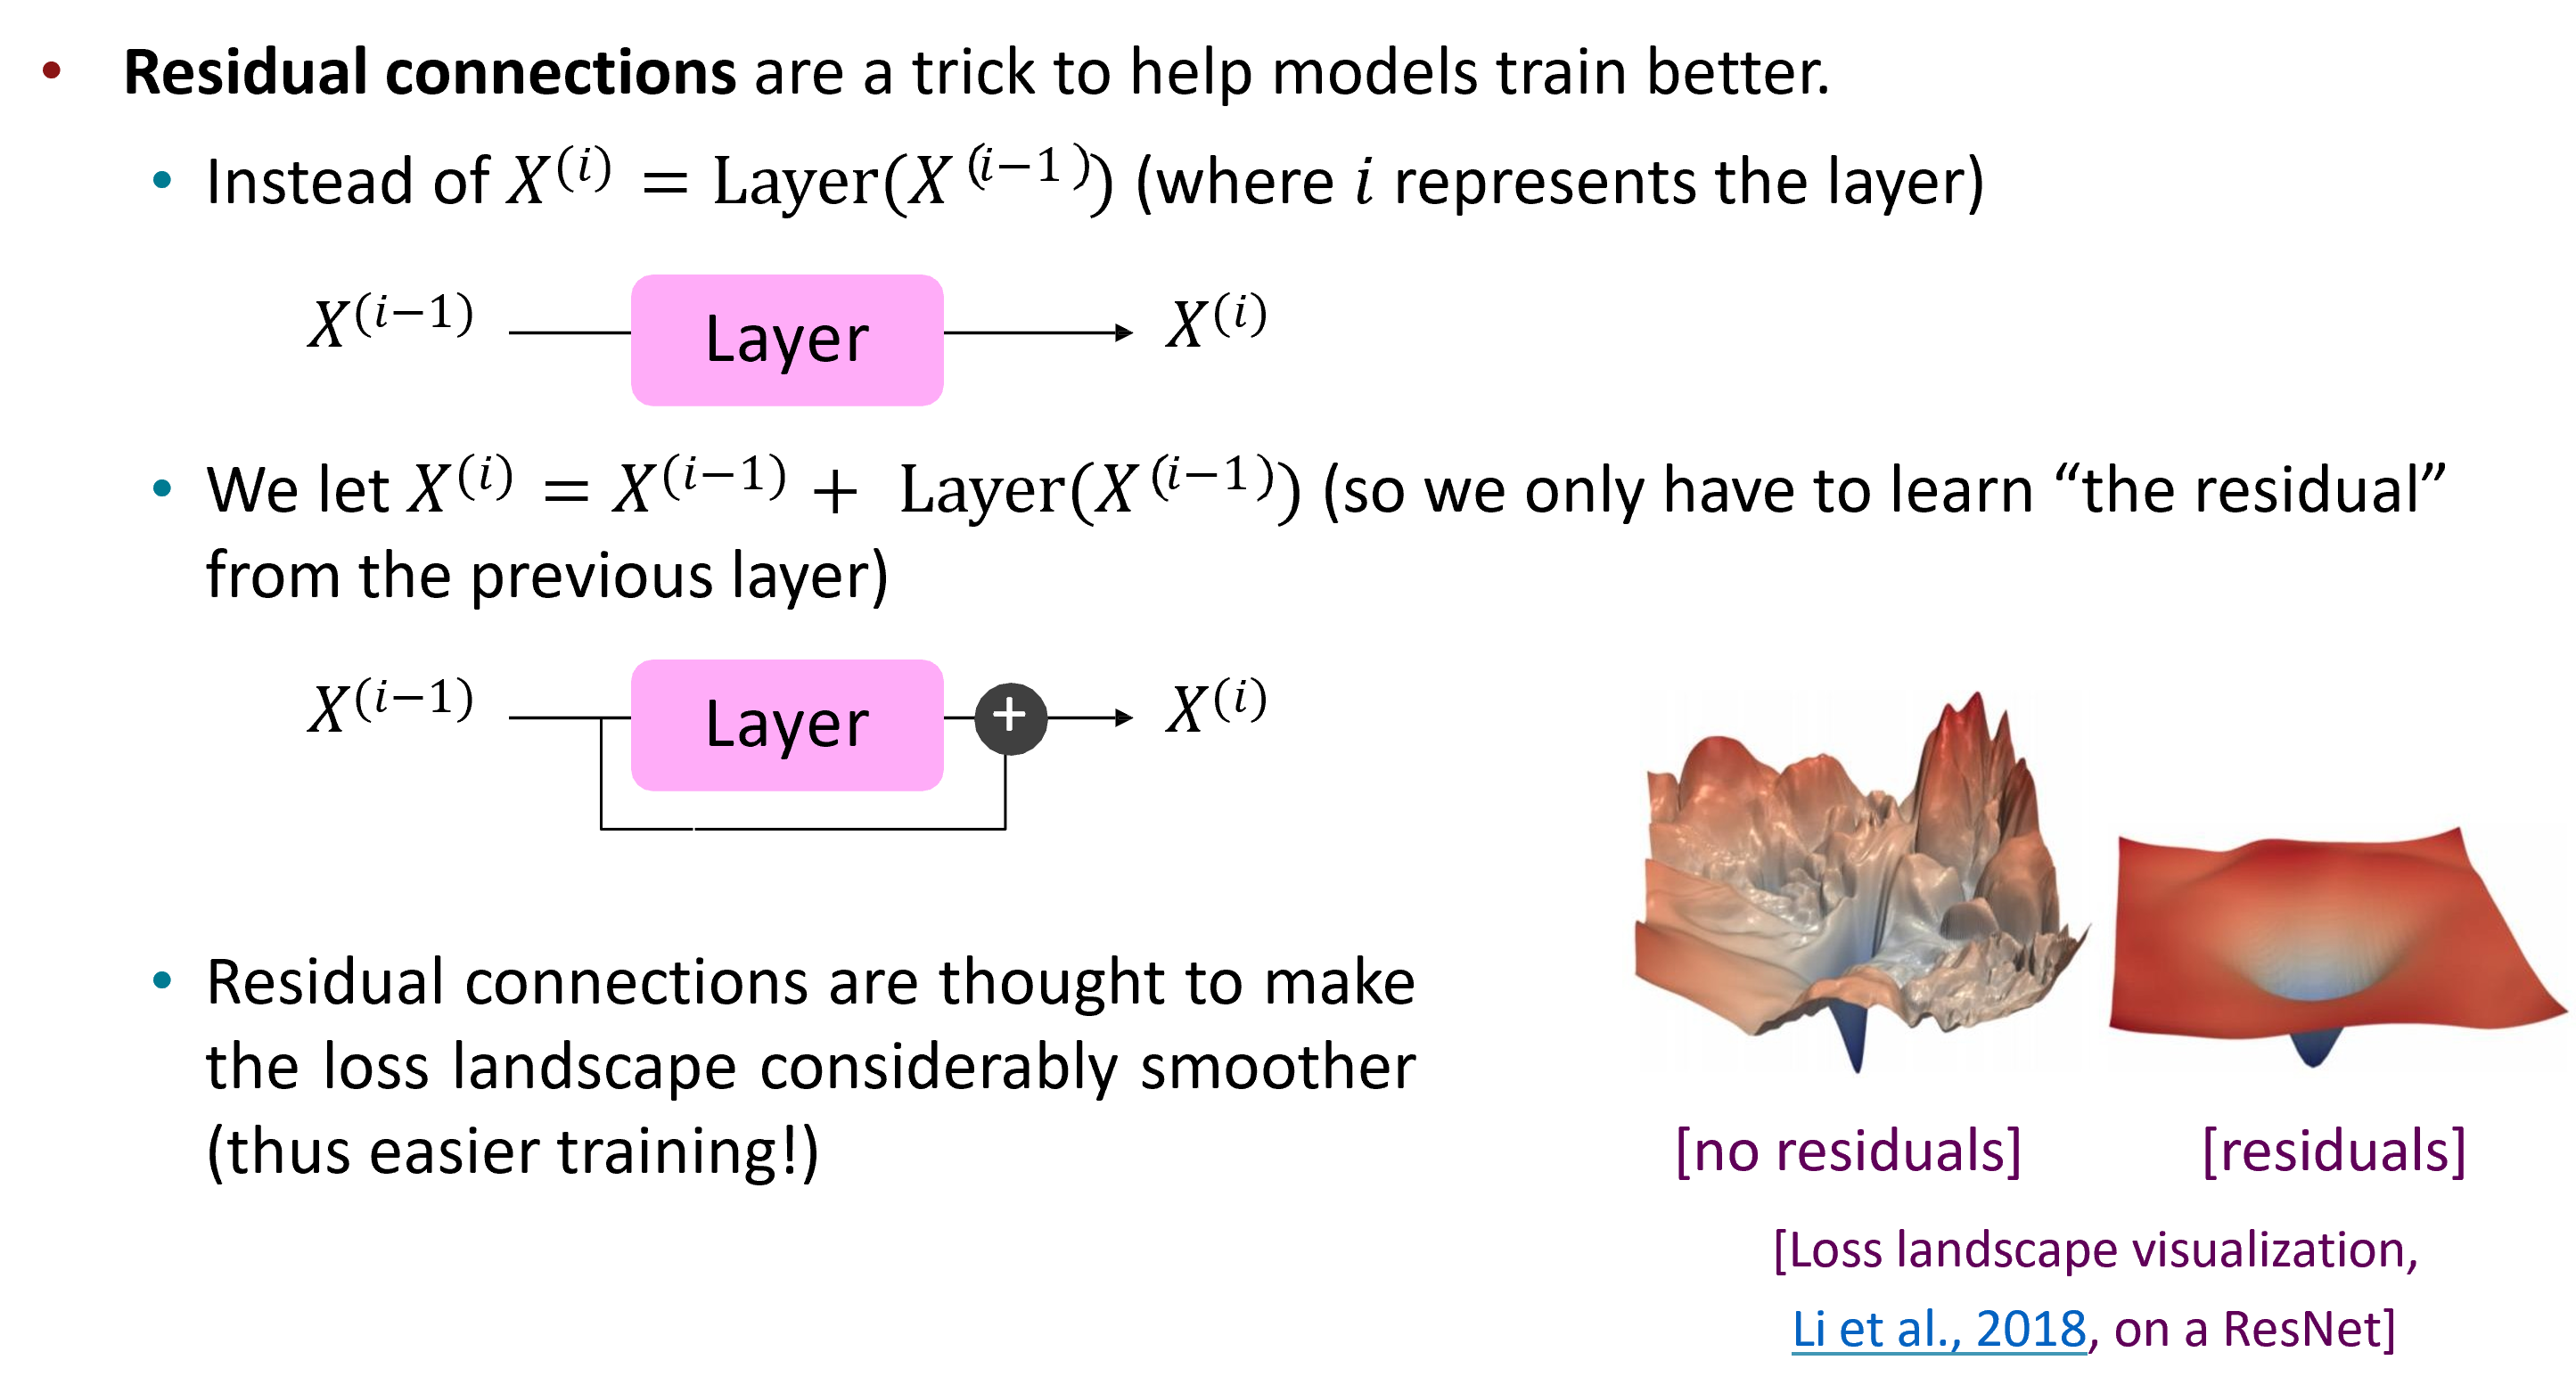
\includegraphics[width=\linewidth,keepaspectratio]{bert82}
			% \end{center}		
			
		
			% % {\tiny (Ref: John Hewitt)}

% \end{frame}

% %%%%%%%%%%%%%%%%%%%%%%%%%%%%%%%%%%%%%%%%%%%%%%%%%%%%%%%%%%%
% \begin{frame}[fragile]\frametitle{Layer normalization}
% The Transformer Encoder: Layer normalization [Ba et al., 2016]
			
			% \begin{center}
			% 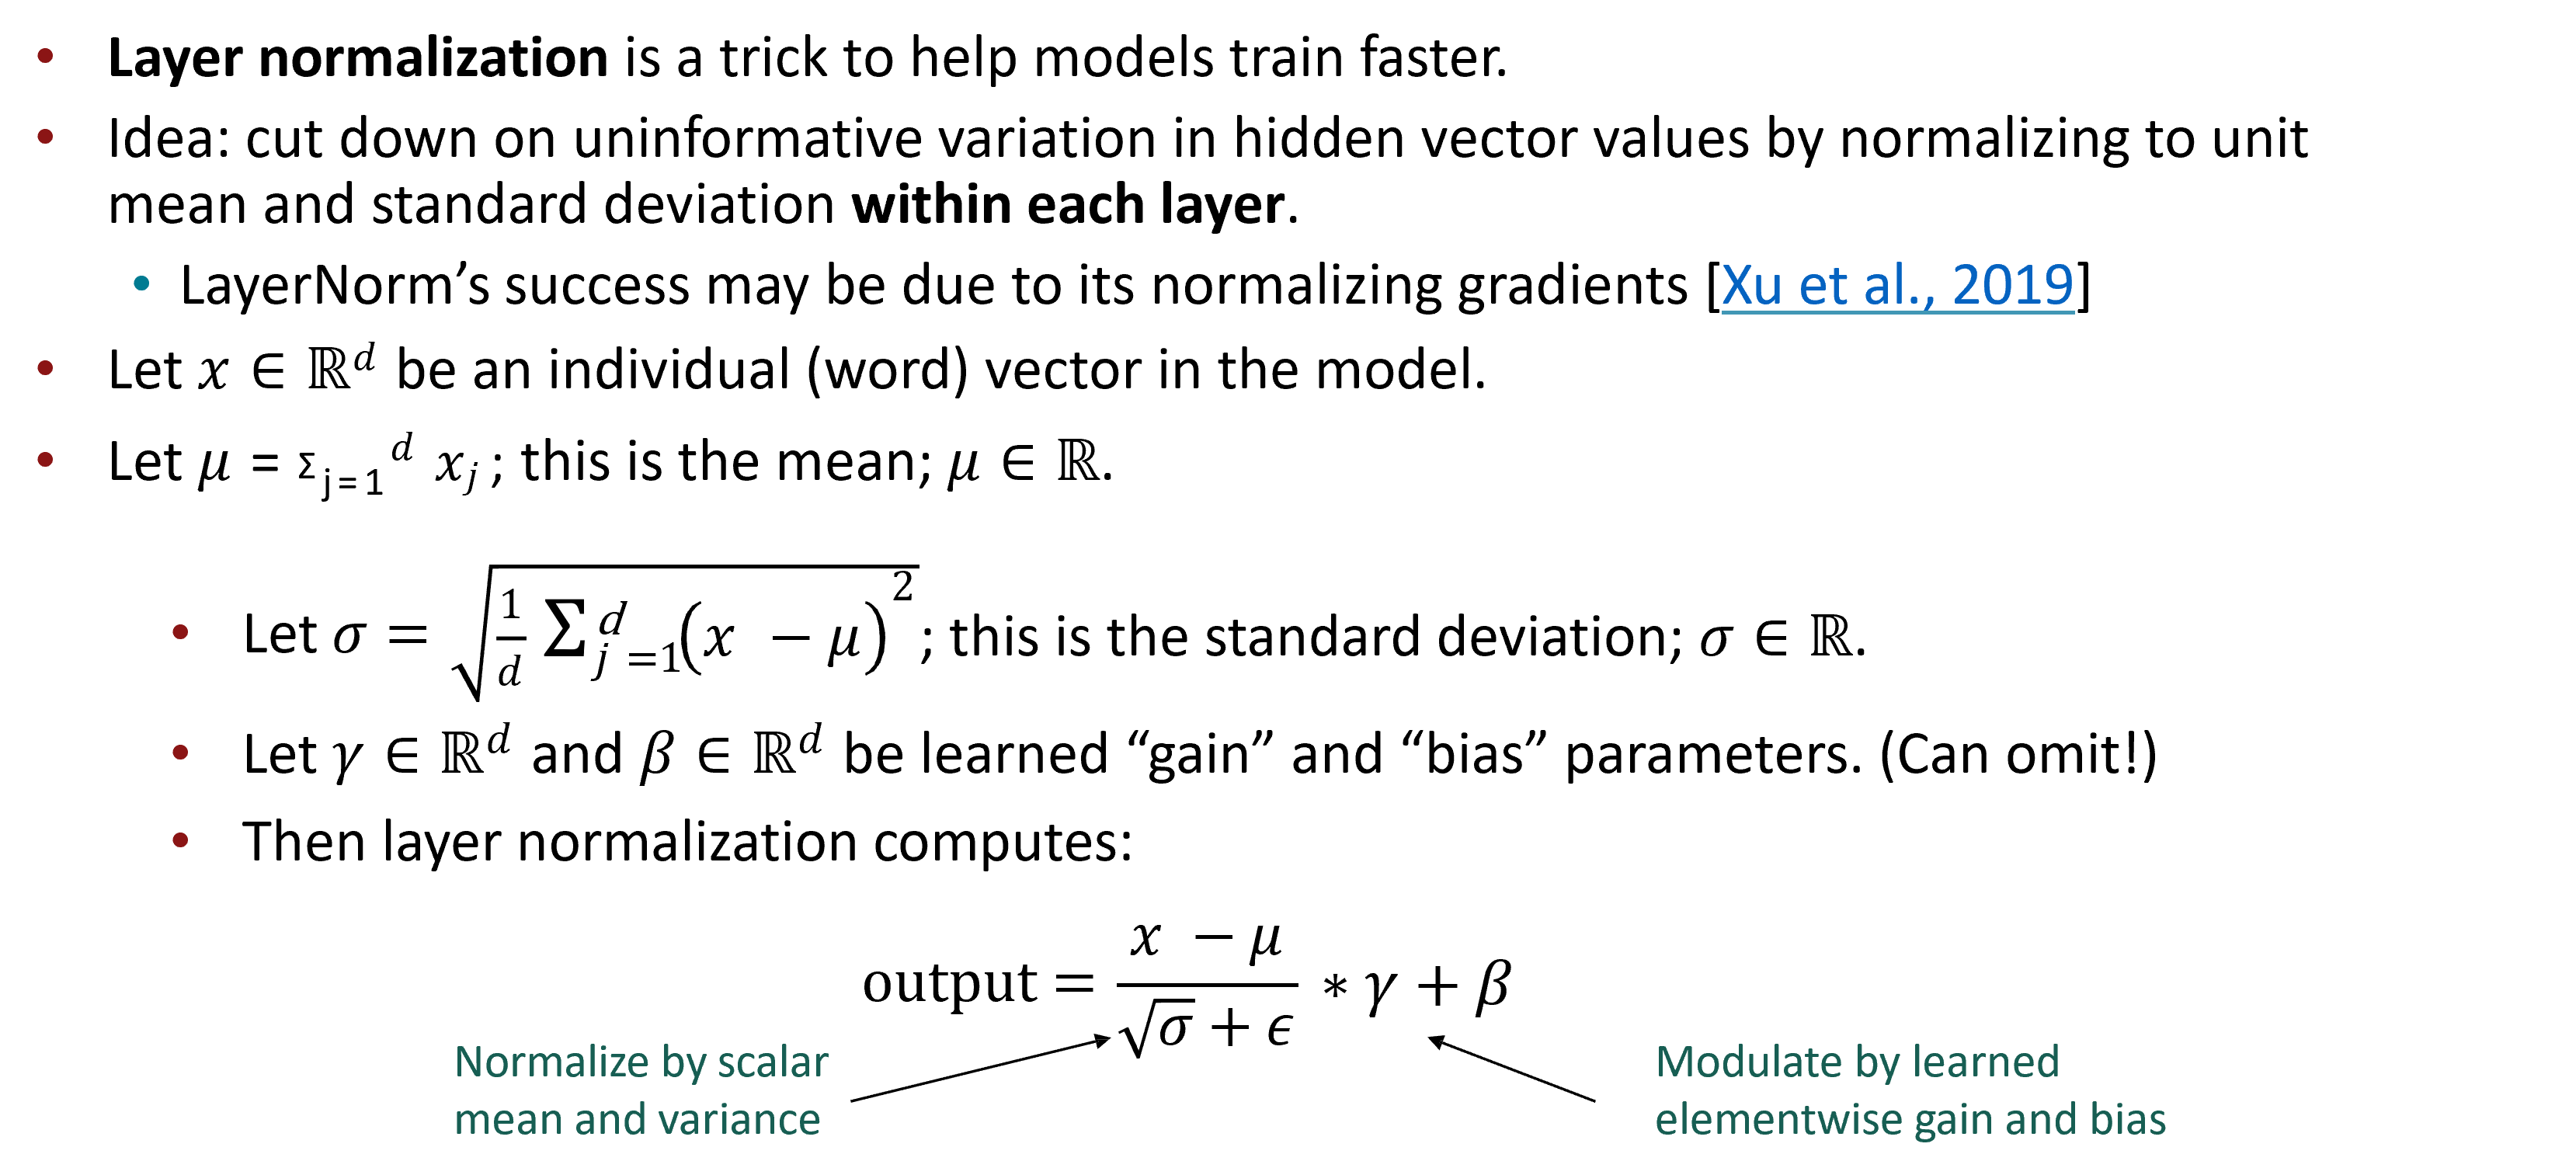
\includegraphics[width=\linewidth,keepaspectratio]{bert83}
			% \end{center}		
			
		
			% % {\tiny (Ref: John Hewitt)}

% \end{frame}

% %%%%%%%%%%%%%%%%%%%%%%%%%%%%%%%%%%%%%%%%%%%%%%%%%%%%%%%%%%%
% \begin{frame}[fragile]\frametitle{ Scaled Dot Product}

			% The Transformer Encoder: Scaled Dot Product [Vaswani et al., 2017]
			% \begin{center}
			% 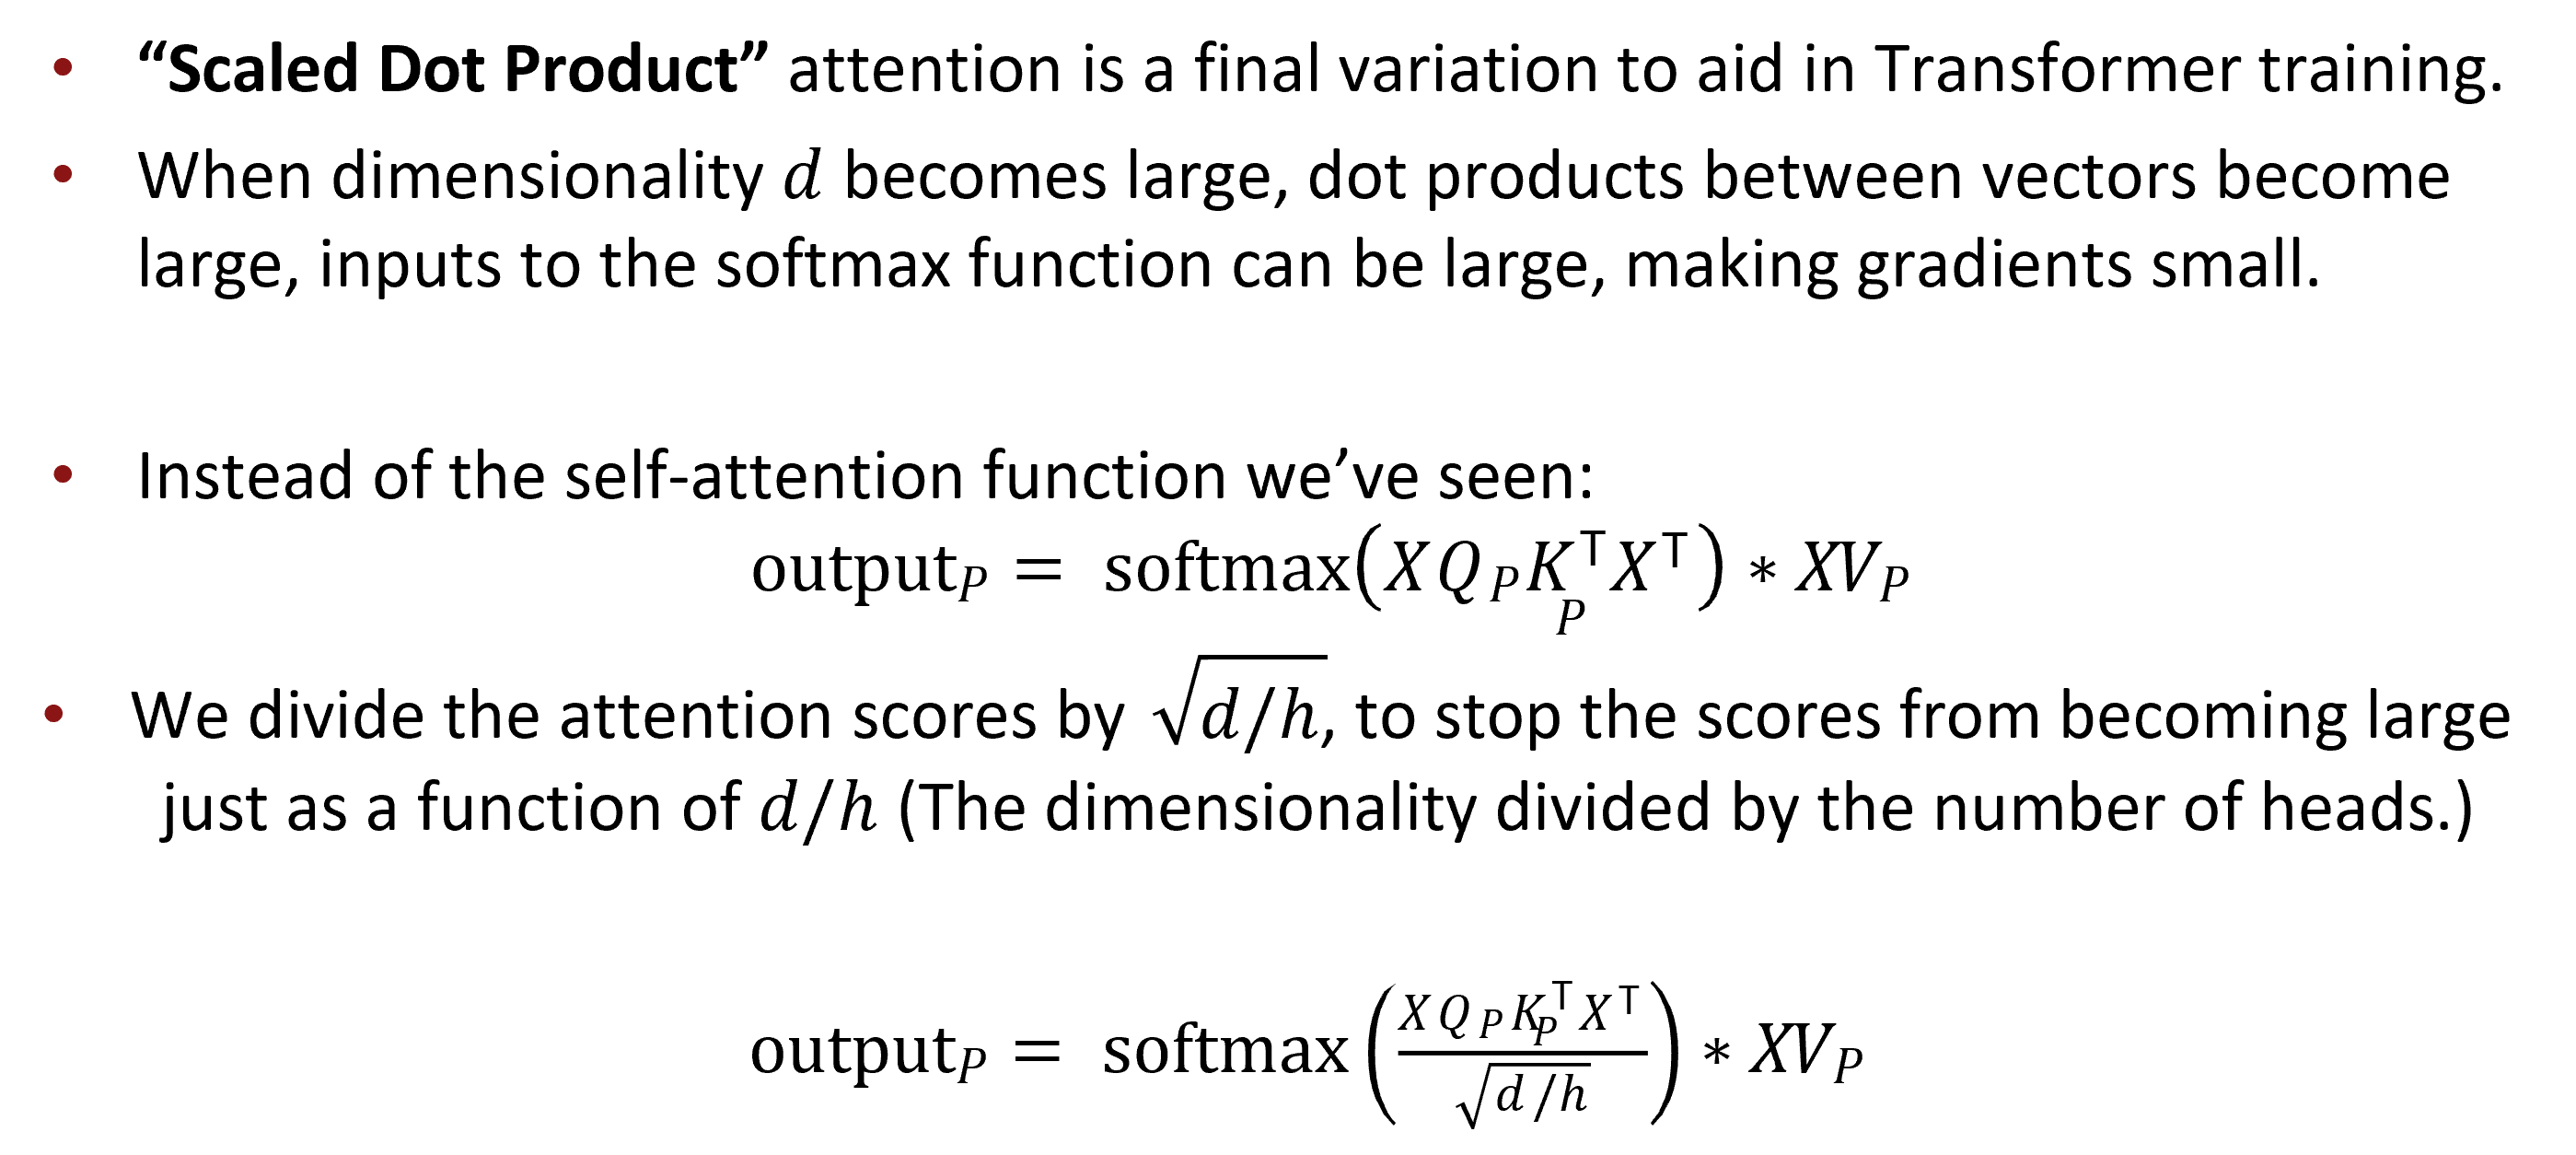
\includegraphics[width=\linewidth,keepaspectratio]{bert84}
			% \end{center}		
			
		
			% % {\tiny (Ref: John Hewitt)}

% \end{frame}

% %%%%%%%%%%%%%%%%%%%%%%%%%%%%%%%%%%%%%%%%%%%%%%%%%%%%%%%%%%%
% \begin{frame}[fragile]\frametitle{Scaled Dot Product}

% The Transformer Encoder: Scaled Dot Product [Vaswani et al., 2017]
			
			% \begin{center}
			% 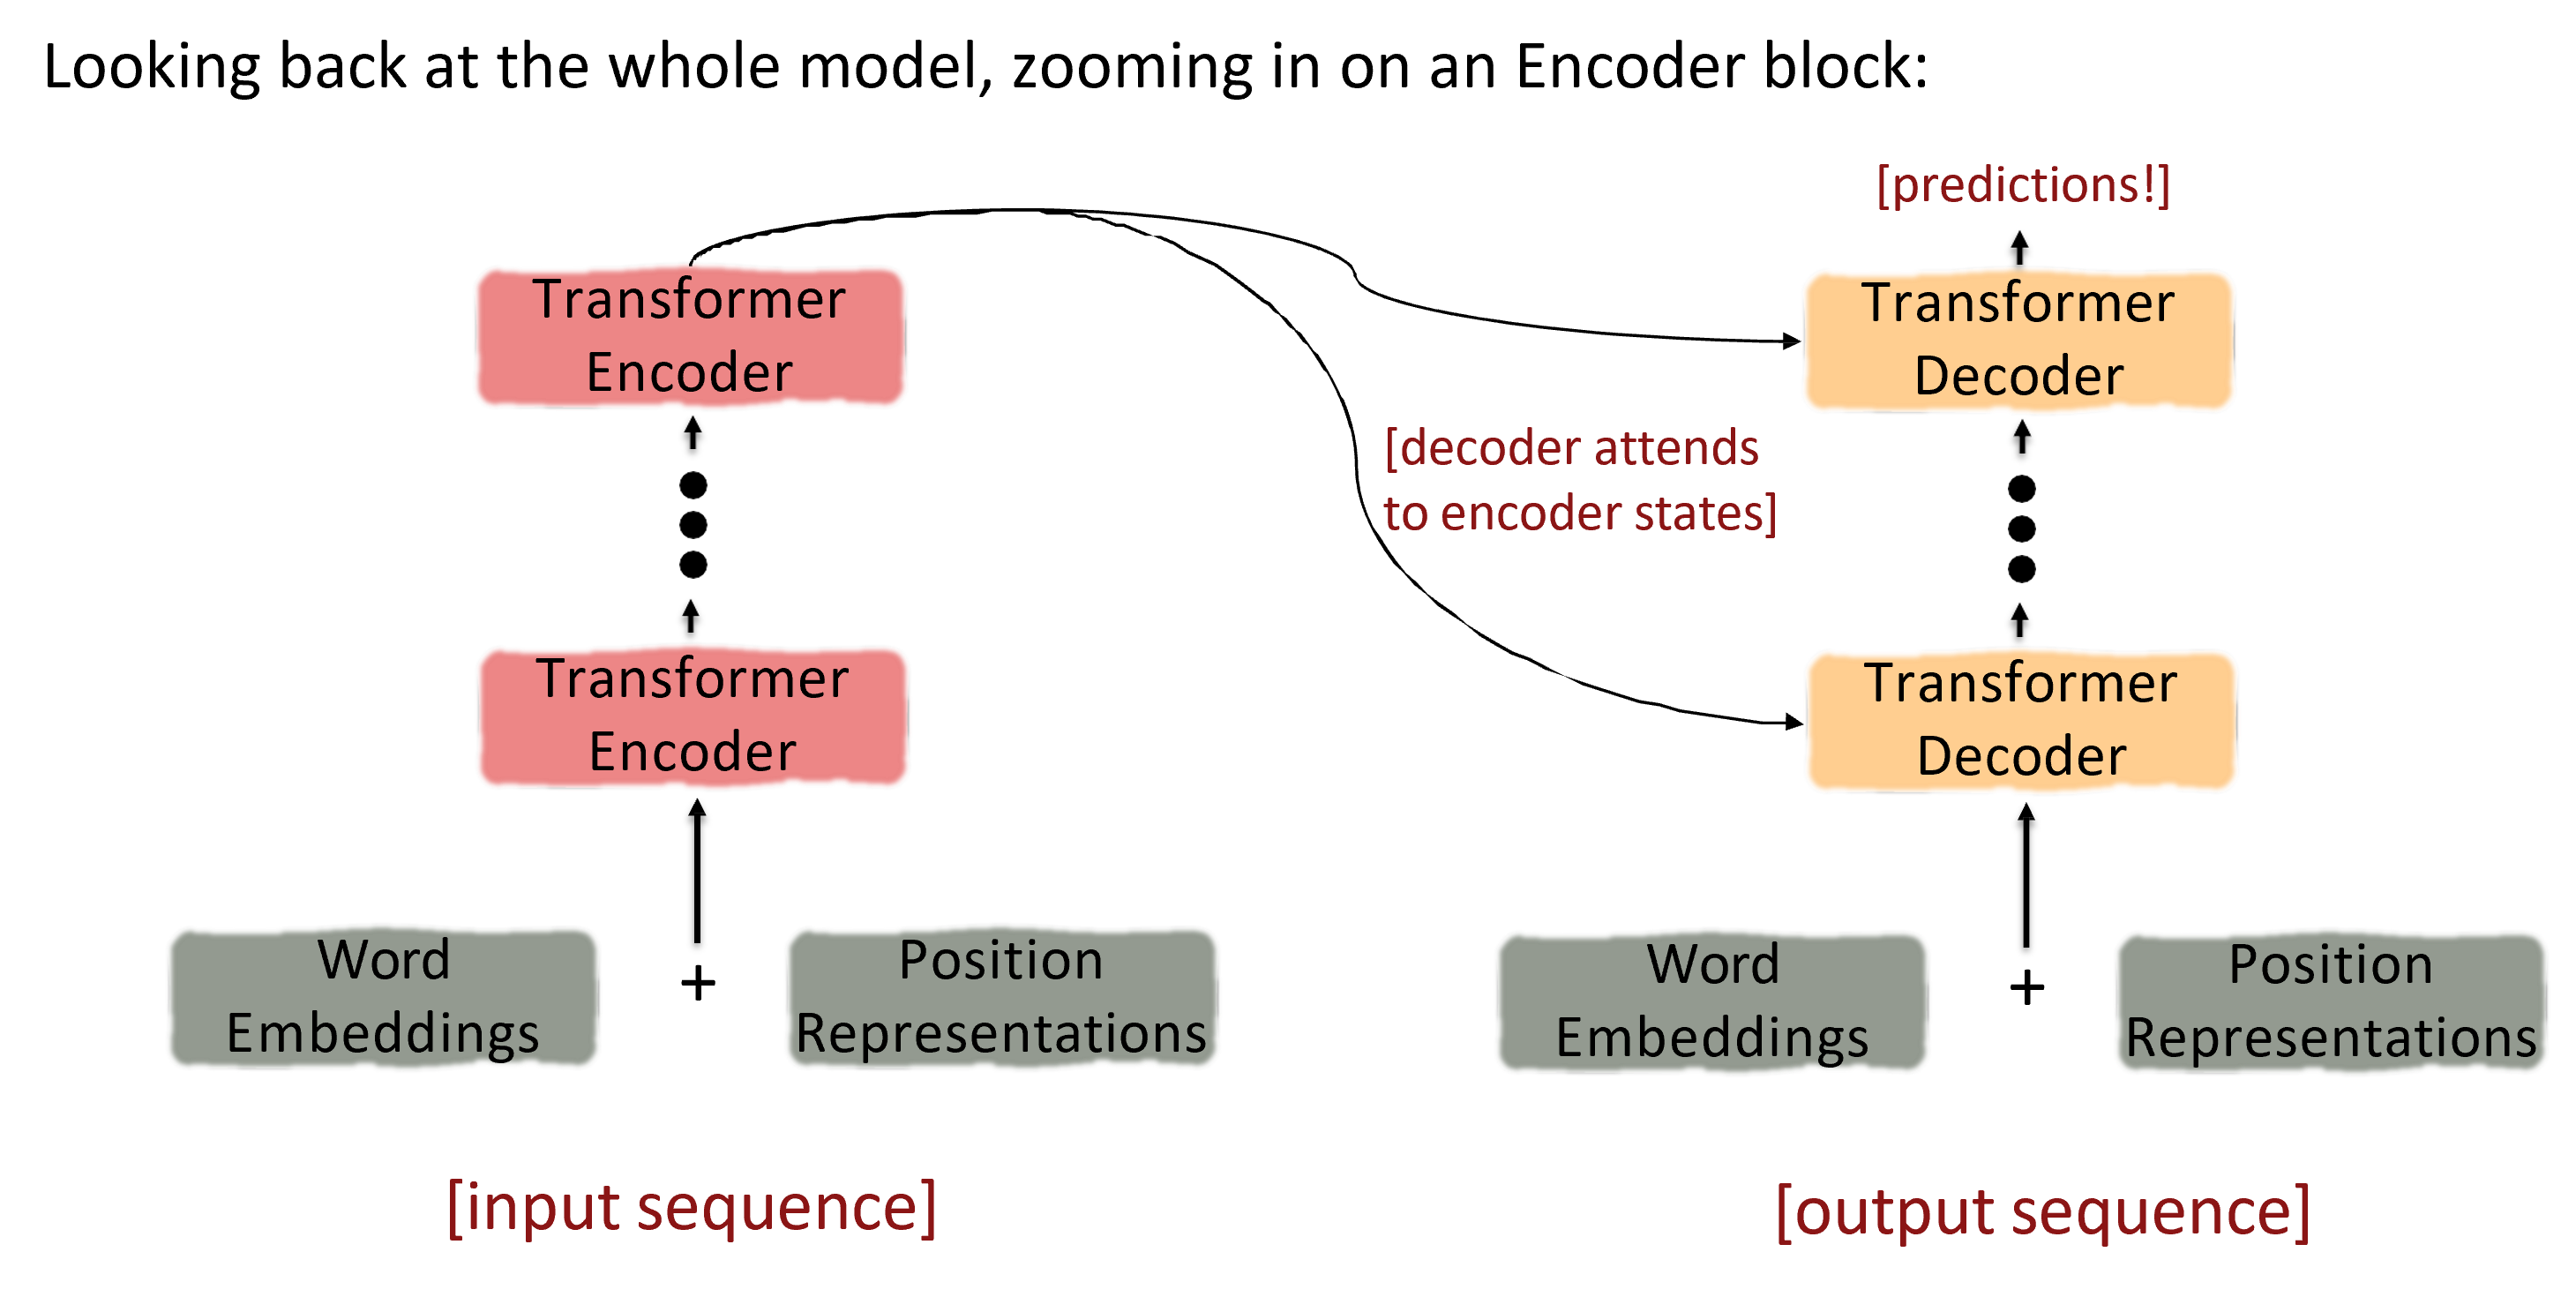
\includegraphics[width=\linewidth,keepaspectratio]{bert85}
			% \end{center}		
			
		
			% % {\tiny (Ref: John Hewitt)}

% \end{frame}

% %%%%%%%%%%%%%%%%%%%%%%%%%%%%%%%%%%%%%%%%%%%%%%%%%%%%%%%%%%%
% \begin{frame}[fragile]\frametitle{Scaled Dot Product}

			% The Transformer Encoder: Scaled Dot Product [Vaswani et al., 2017]
			
			% \begin{center}
			% 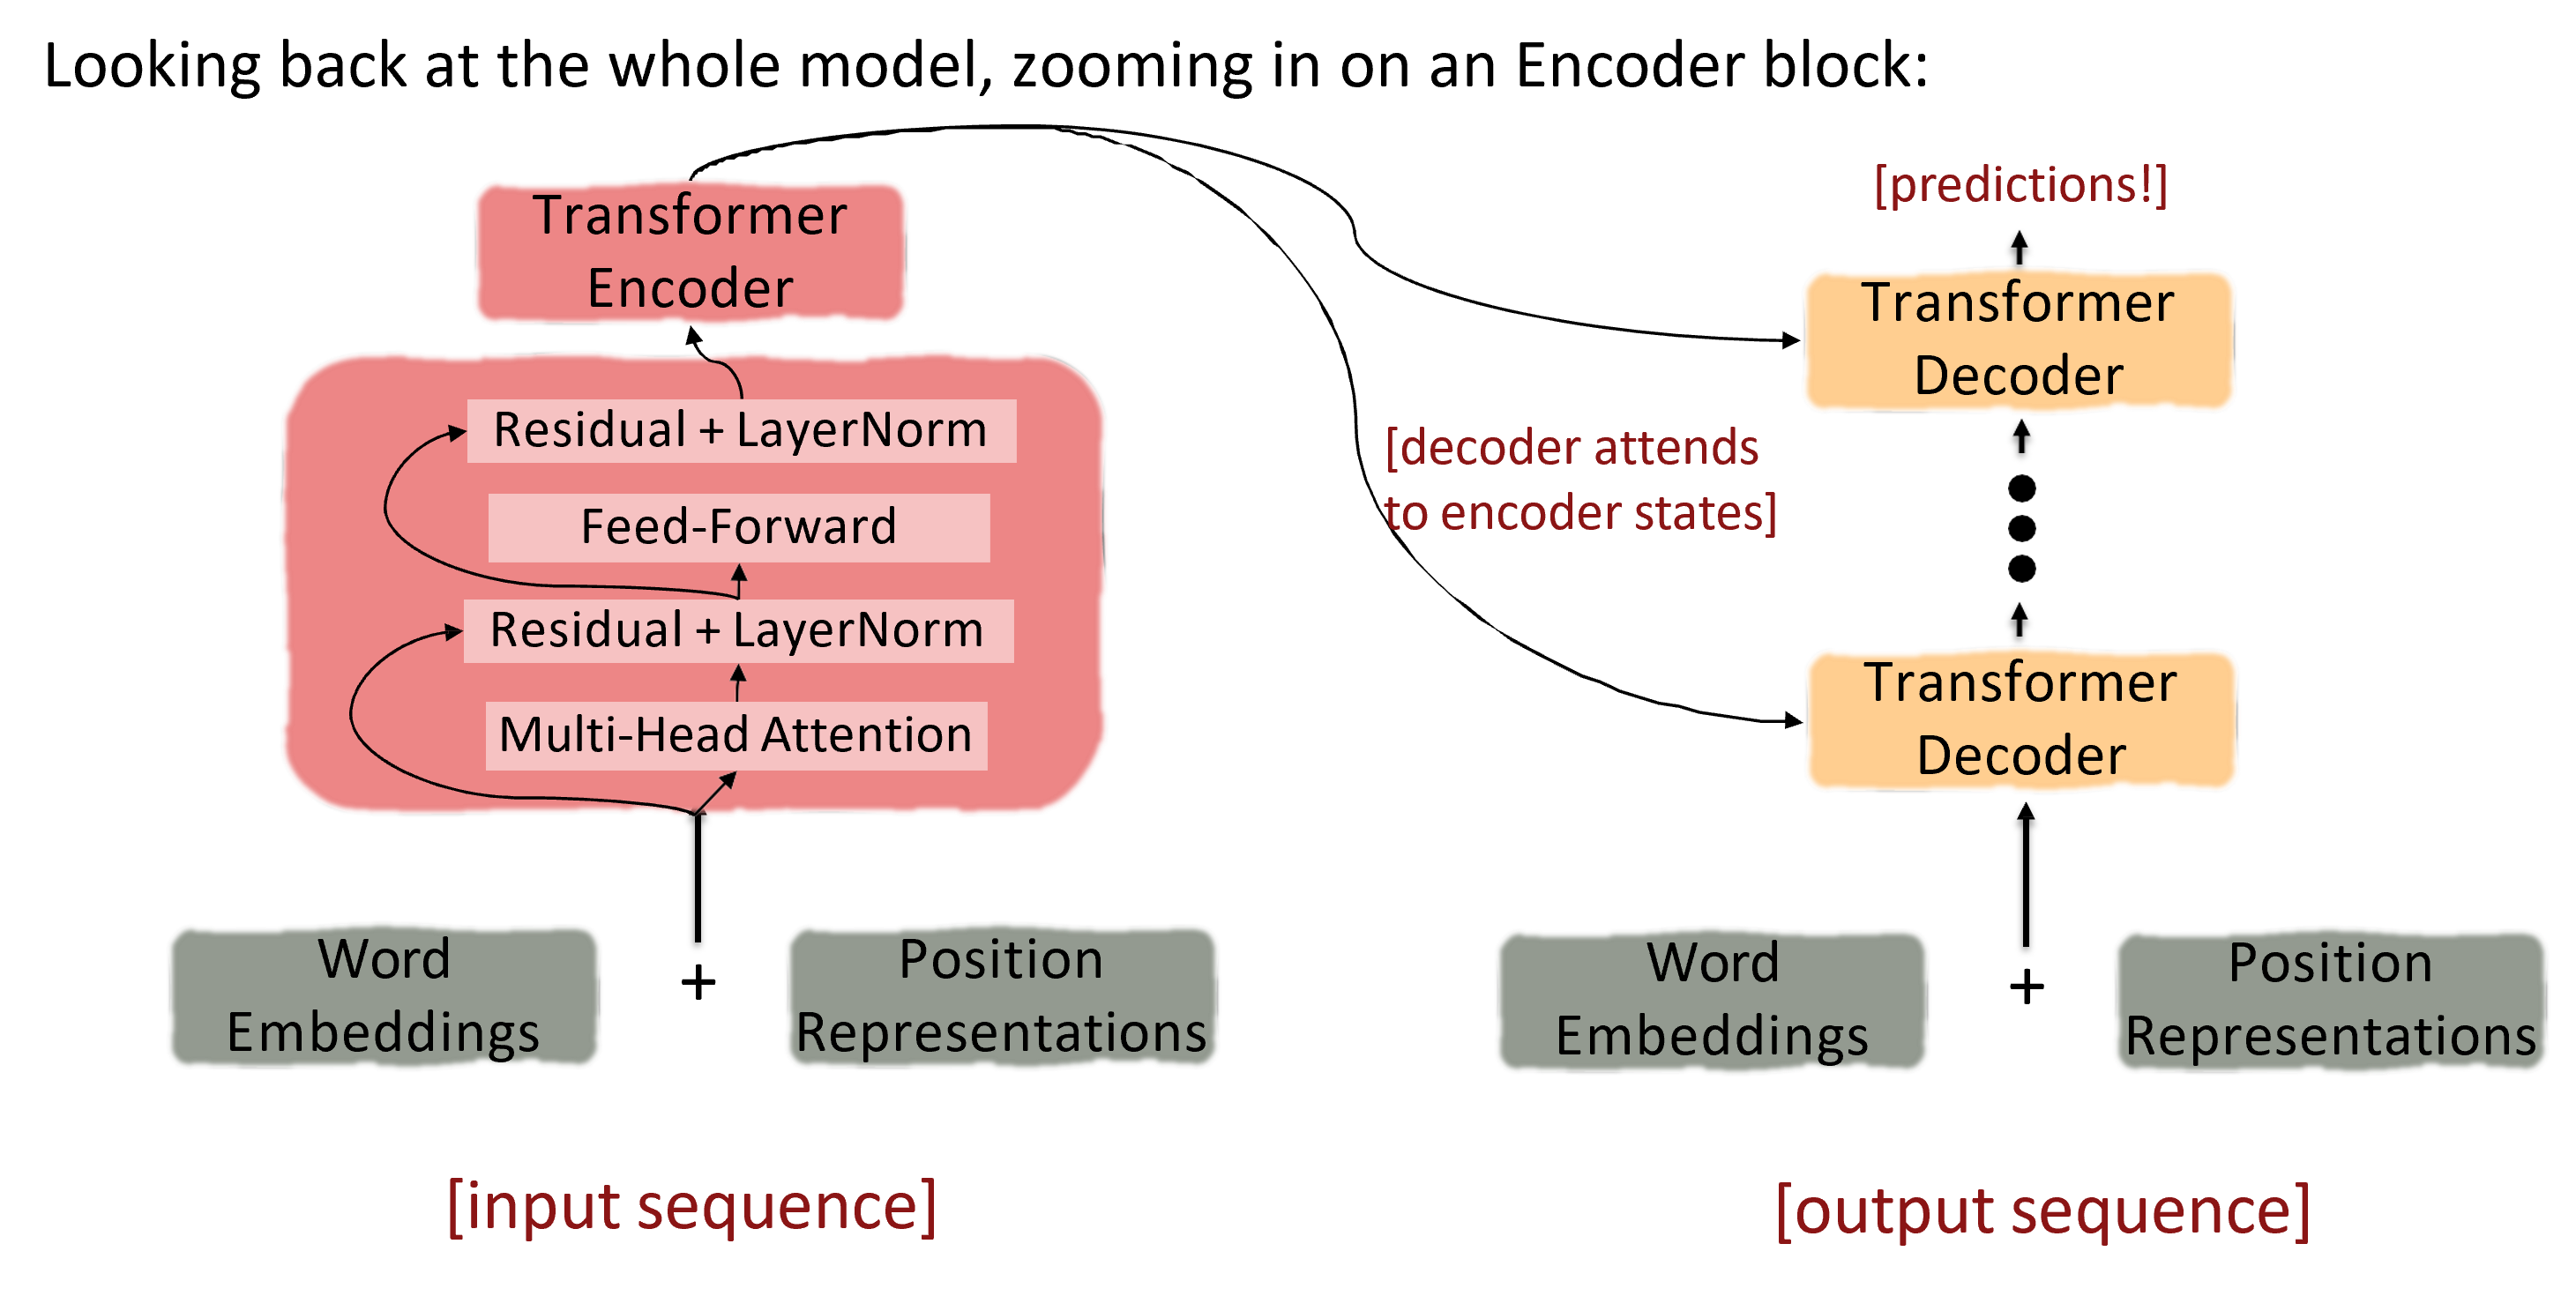
\includegraphics[width=\linewidth,keepaspectratio]{bert86}
			% \end{center}		
			
		
			% % {\tiny (Ref: John Hewitt)}

% \end{frame}

% %%%%%%%%%%%%%%%%%%%%%%%%%%%%%%%%%%%%%%%%%%%%%%%%%%%%%%%%%%%
% \begin{frame}[fragile]\frametitle{Scaled Dot Product}

						% The Transformer Encoder: Scaled Dot Product [Vaswani et al., 2017]

			% \begin{center}
			% 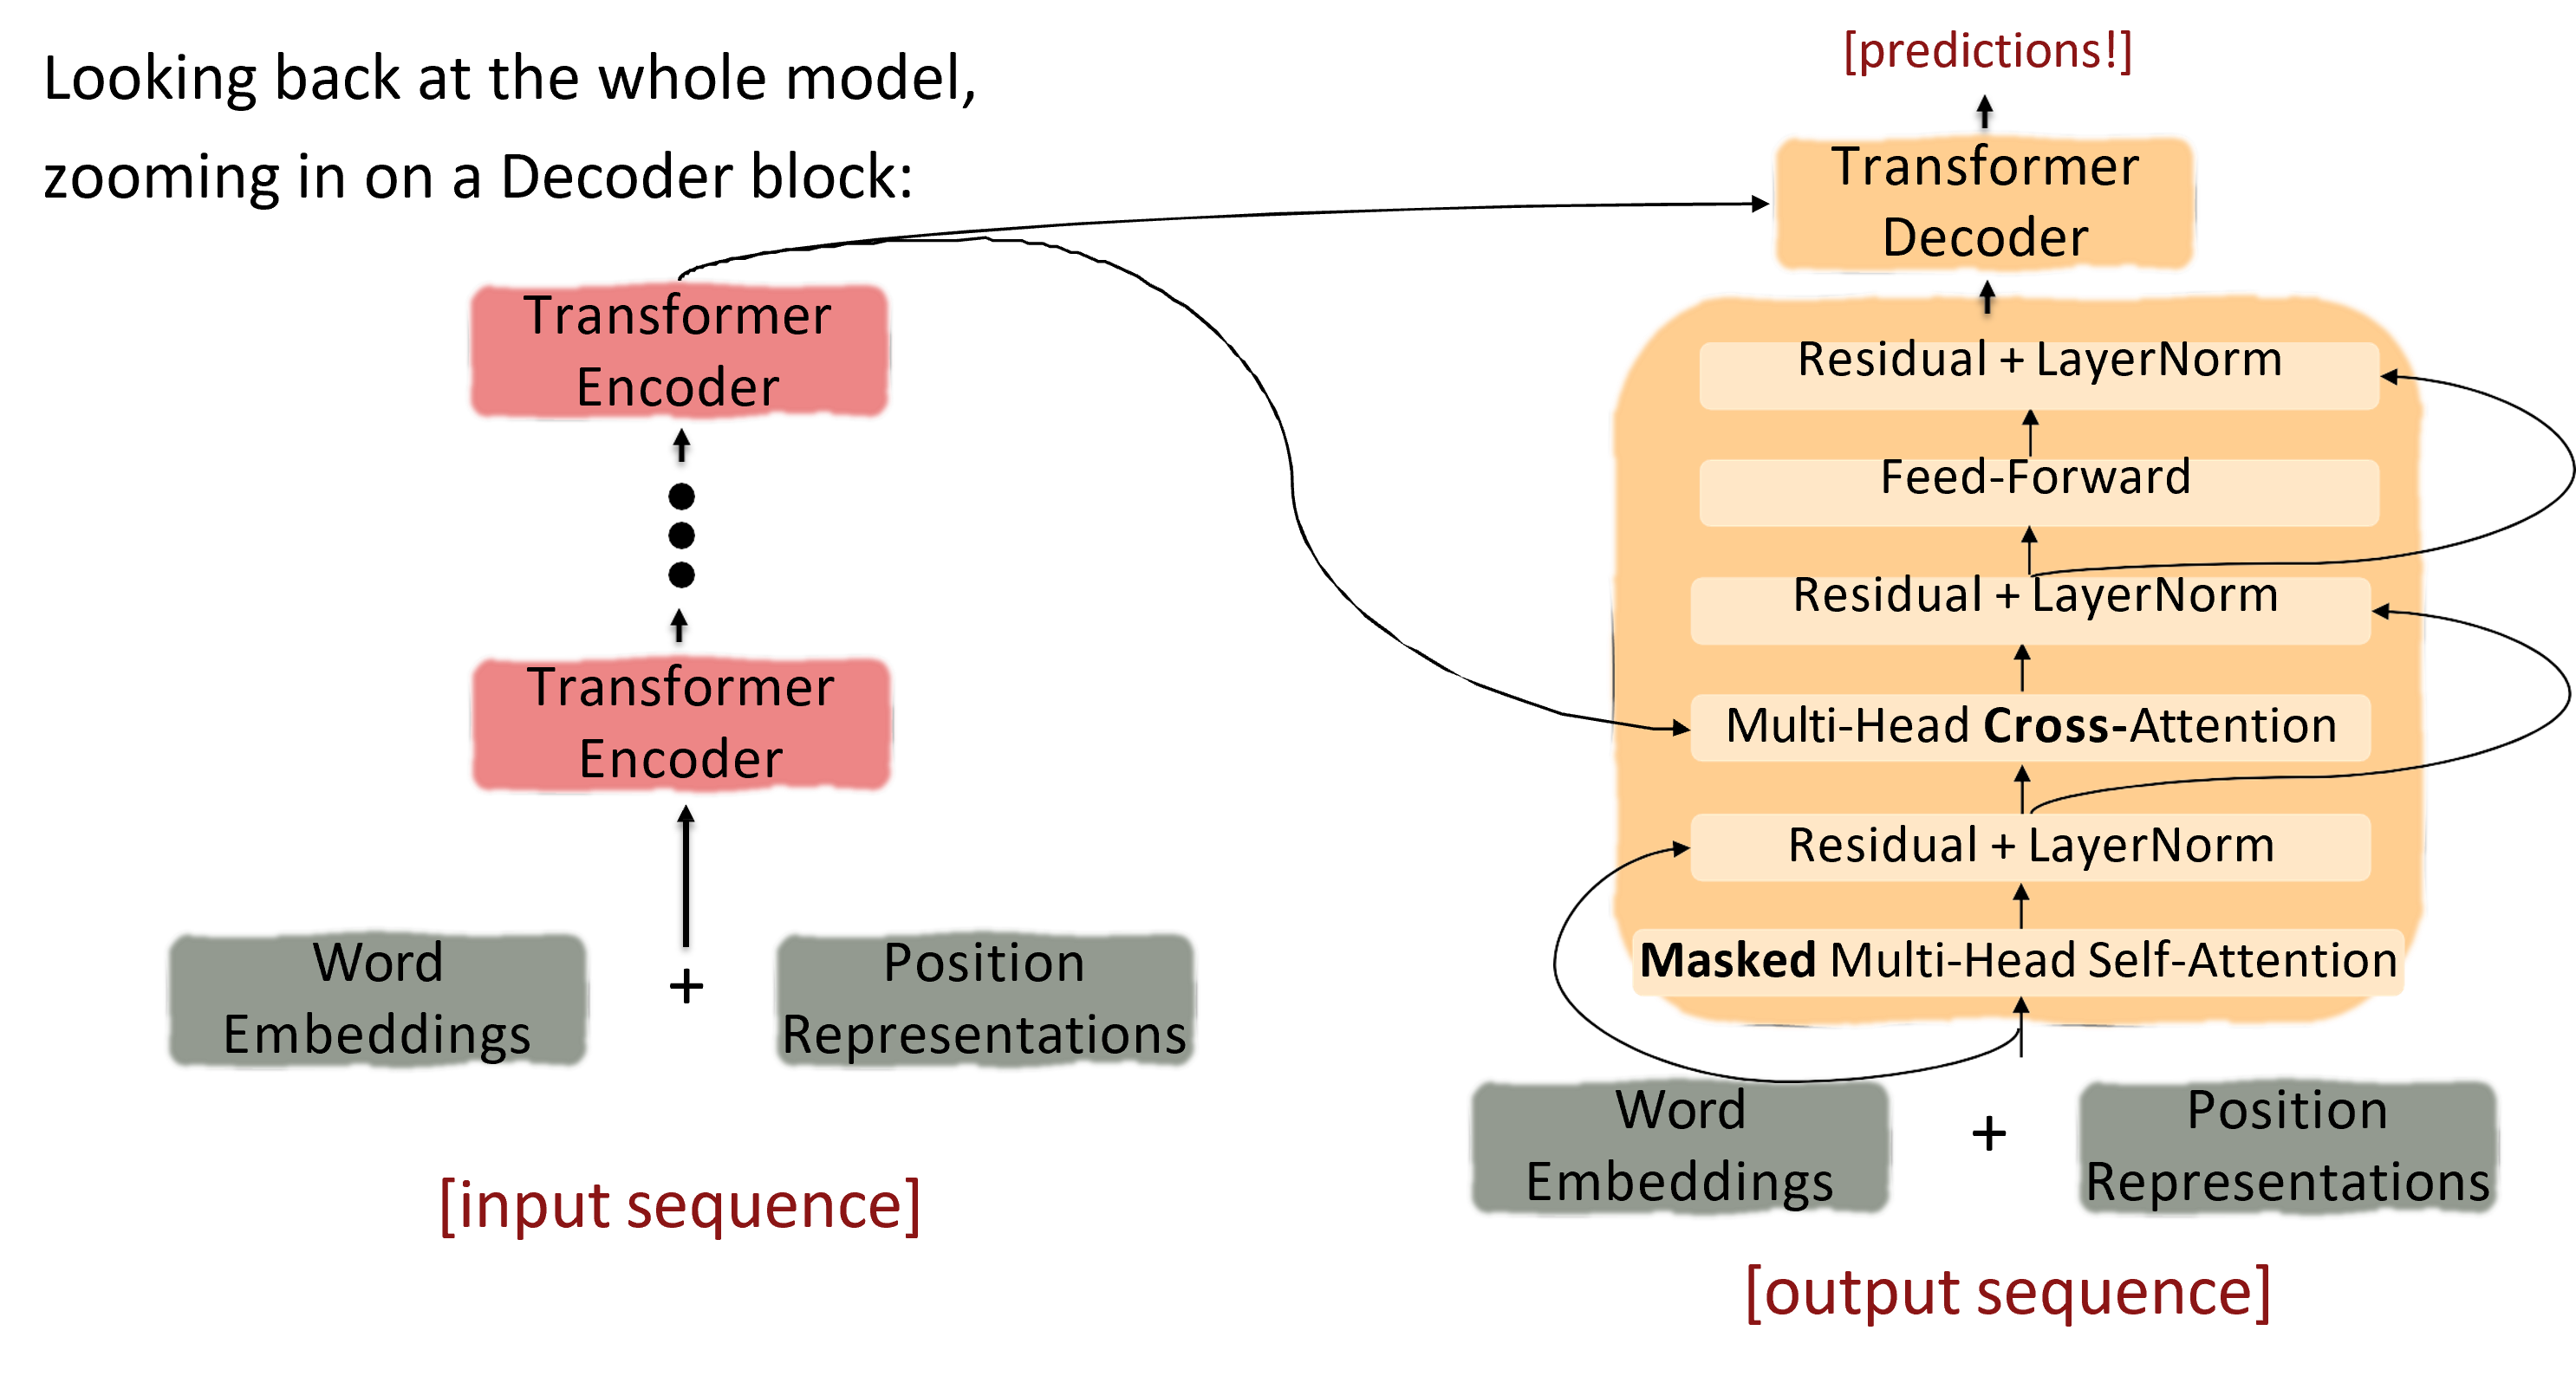
\includegraphics[width=\linewidth,keepaspectratio]{bert87}
			% \end{center}		
			
		
			% % {\tiny (Ref: John Hewitt)}

% \end{frame}

% %%%%%%%%%%%%%%%%%%%%%%%%%%%%%%%%%%%%%%%%%%%%%%%%%%%%%%%%%%%
% \begin{frame}[fragile]\frametitle{Scaled Dot Product}

						% The Transformer Encoder: Scaled Dot Product [Vaswani et al., 2017]

			
			% \begin{center}
			% 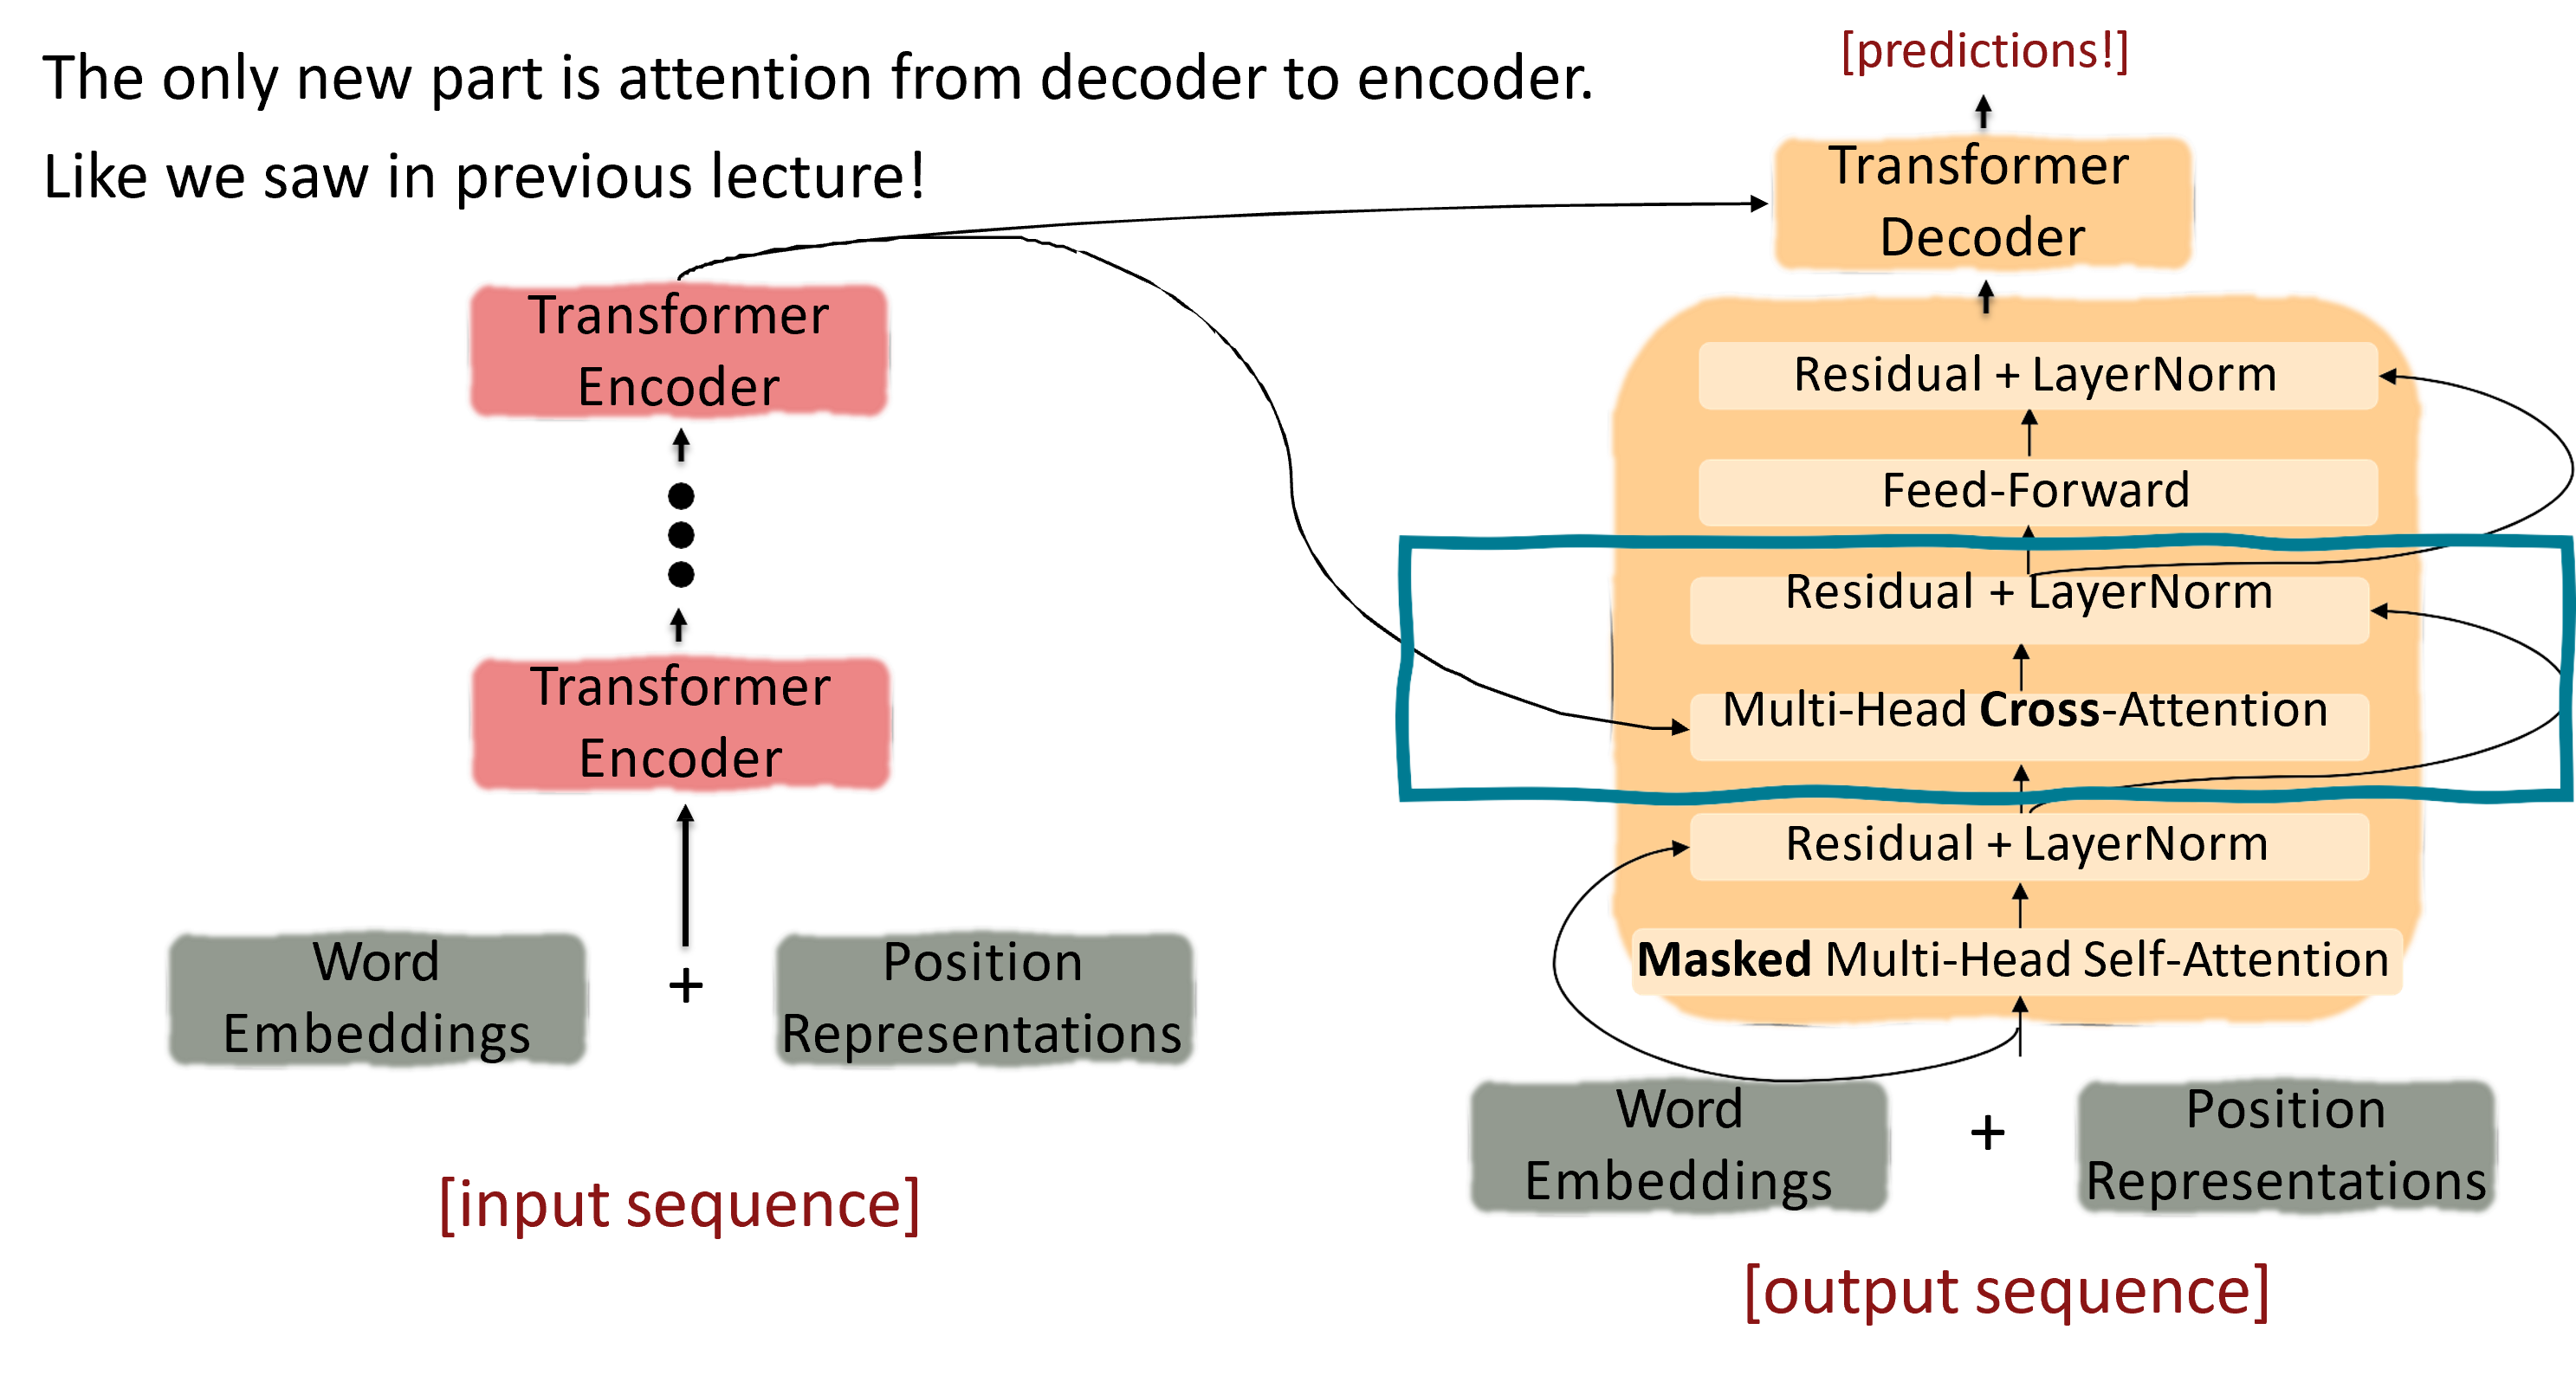
\includegraphics[width=\linewidth,keepaspectratio]{bert88}
			% \end{center}		
			
		
			% % {\tiny (Ref: John Hewitt)}

% \end{frame}

% %%%%%%%%%%%%%%%%%%%%%%%%%%%%%%%%%%%%%%%%%%%%%%%%%%%%%%%%%%%
% \begin{frame}[fragile]\frametitle{Cross-attention}

			% The Transformer Decoder: Cross-attention (details)
			
			% \begin{center}
			% 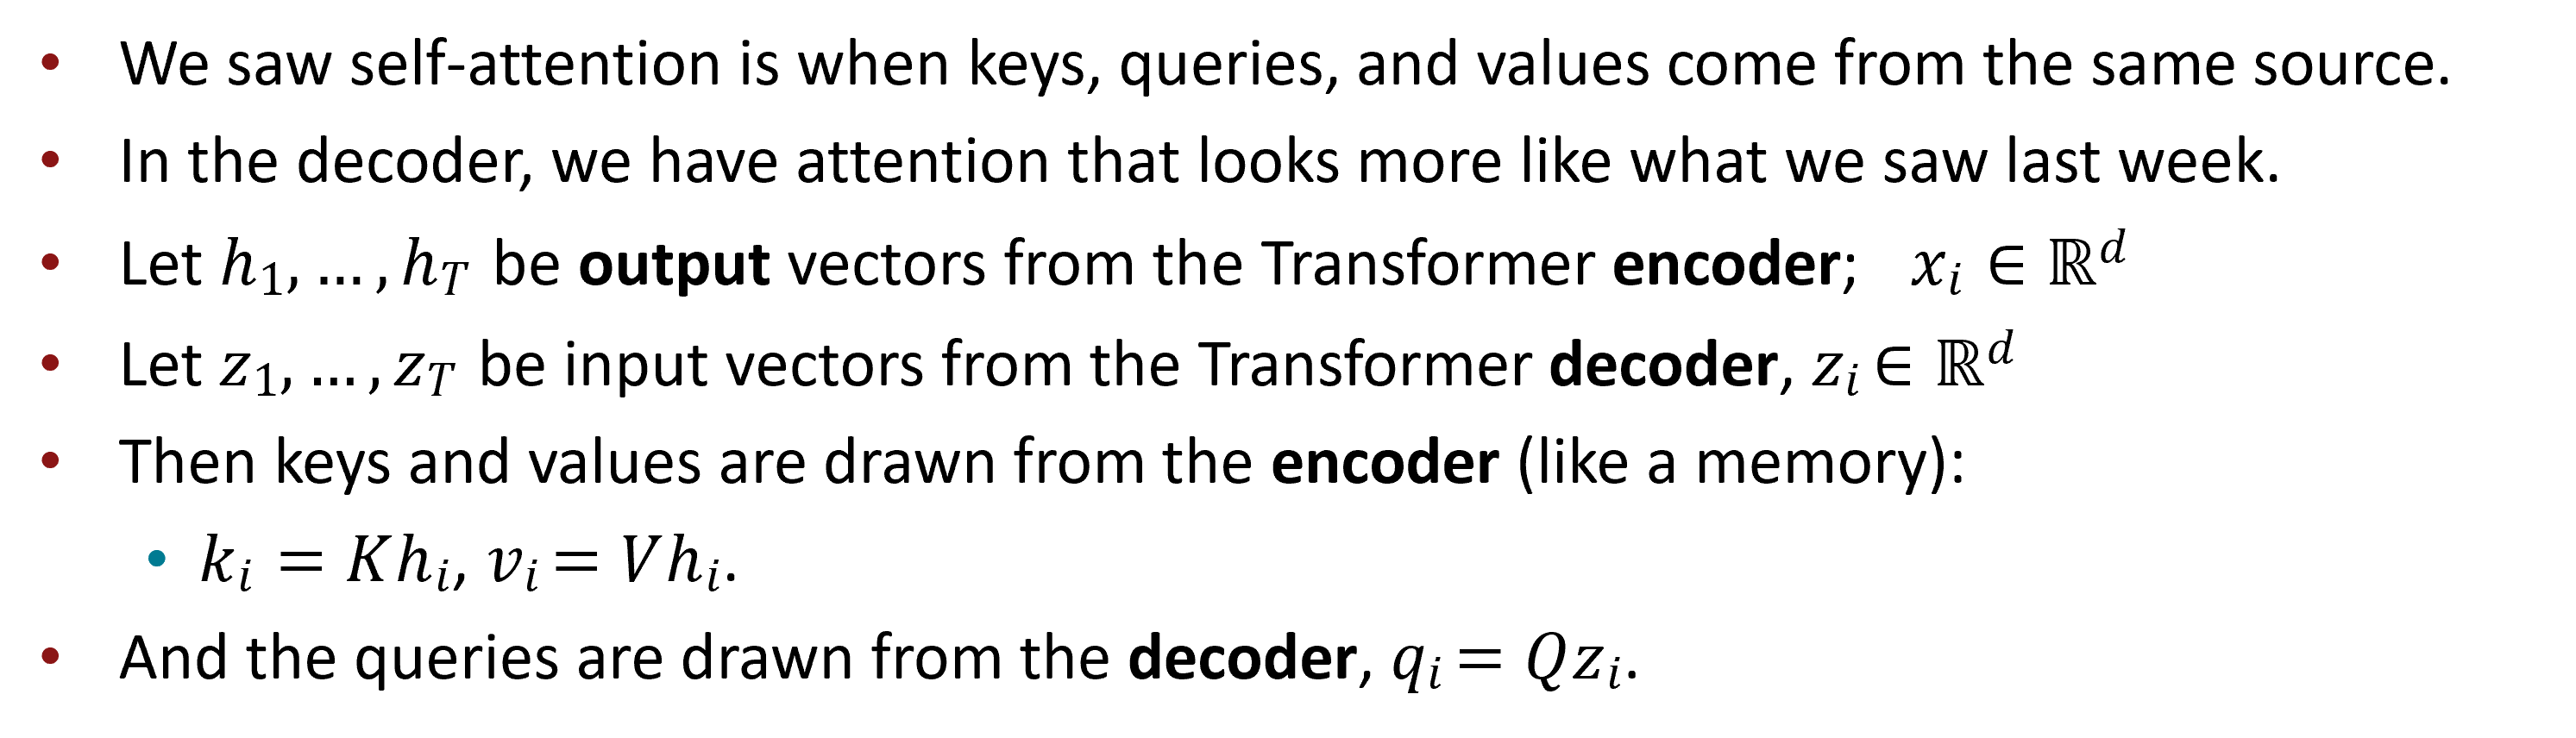
\includegraphics[width=\linewidth,keepaspectratio]{bert89}
			% \end{center}		
			
		
			% % {\tiny (Ref: John Hewitt)}

% \end{frame}

% %%%%%%%%%%%%%%%%%%%%%%%%%%%%%%%%%%%%%%%%%%%%%%%%%%%%%%%%%%%
% \begin{frame}[fragile]\frametitle{Cross-attention}

			% The Transformer Decoder: Cross-attention (details)
			
			% \begin{center}
			% 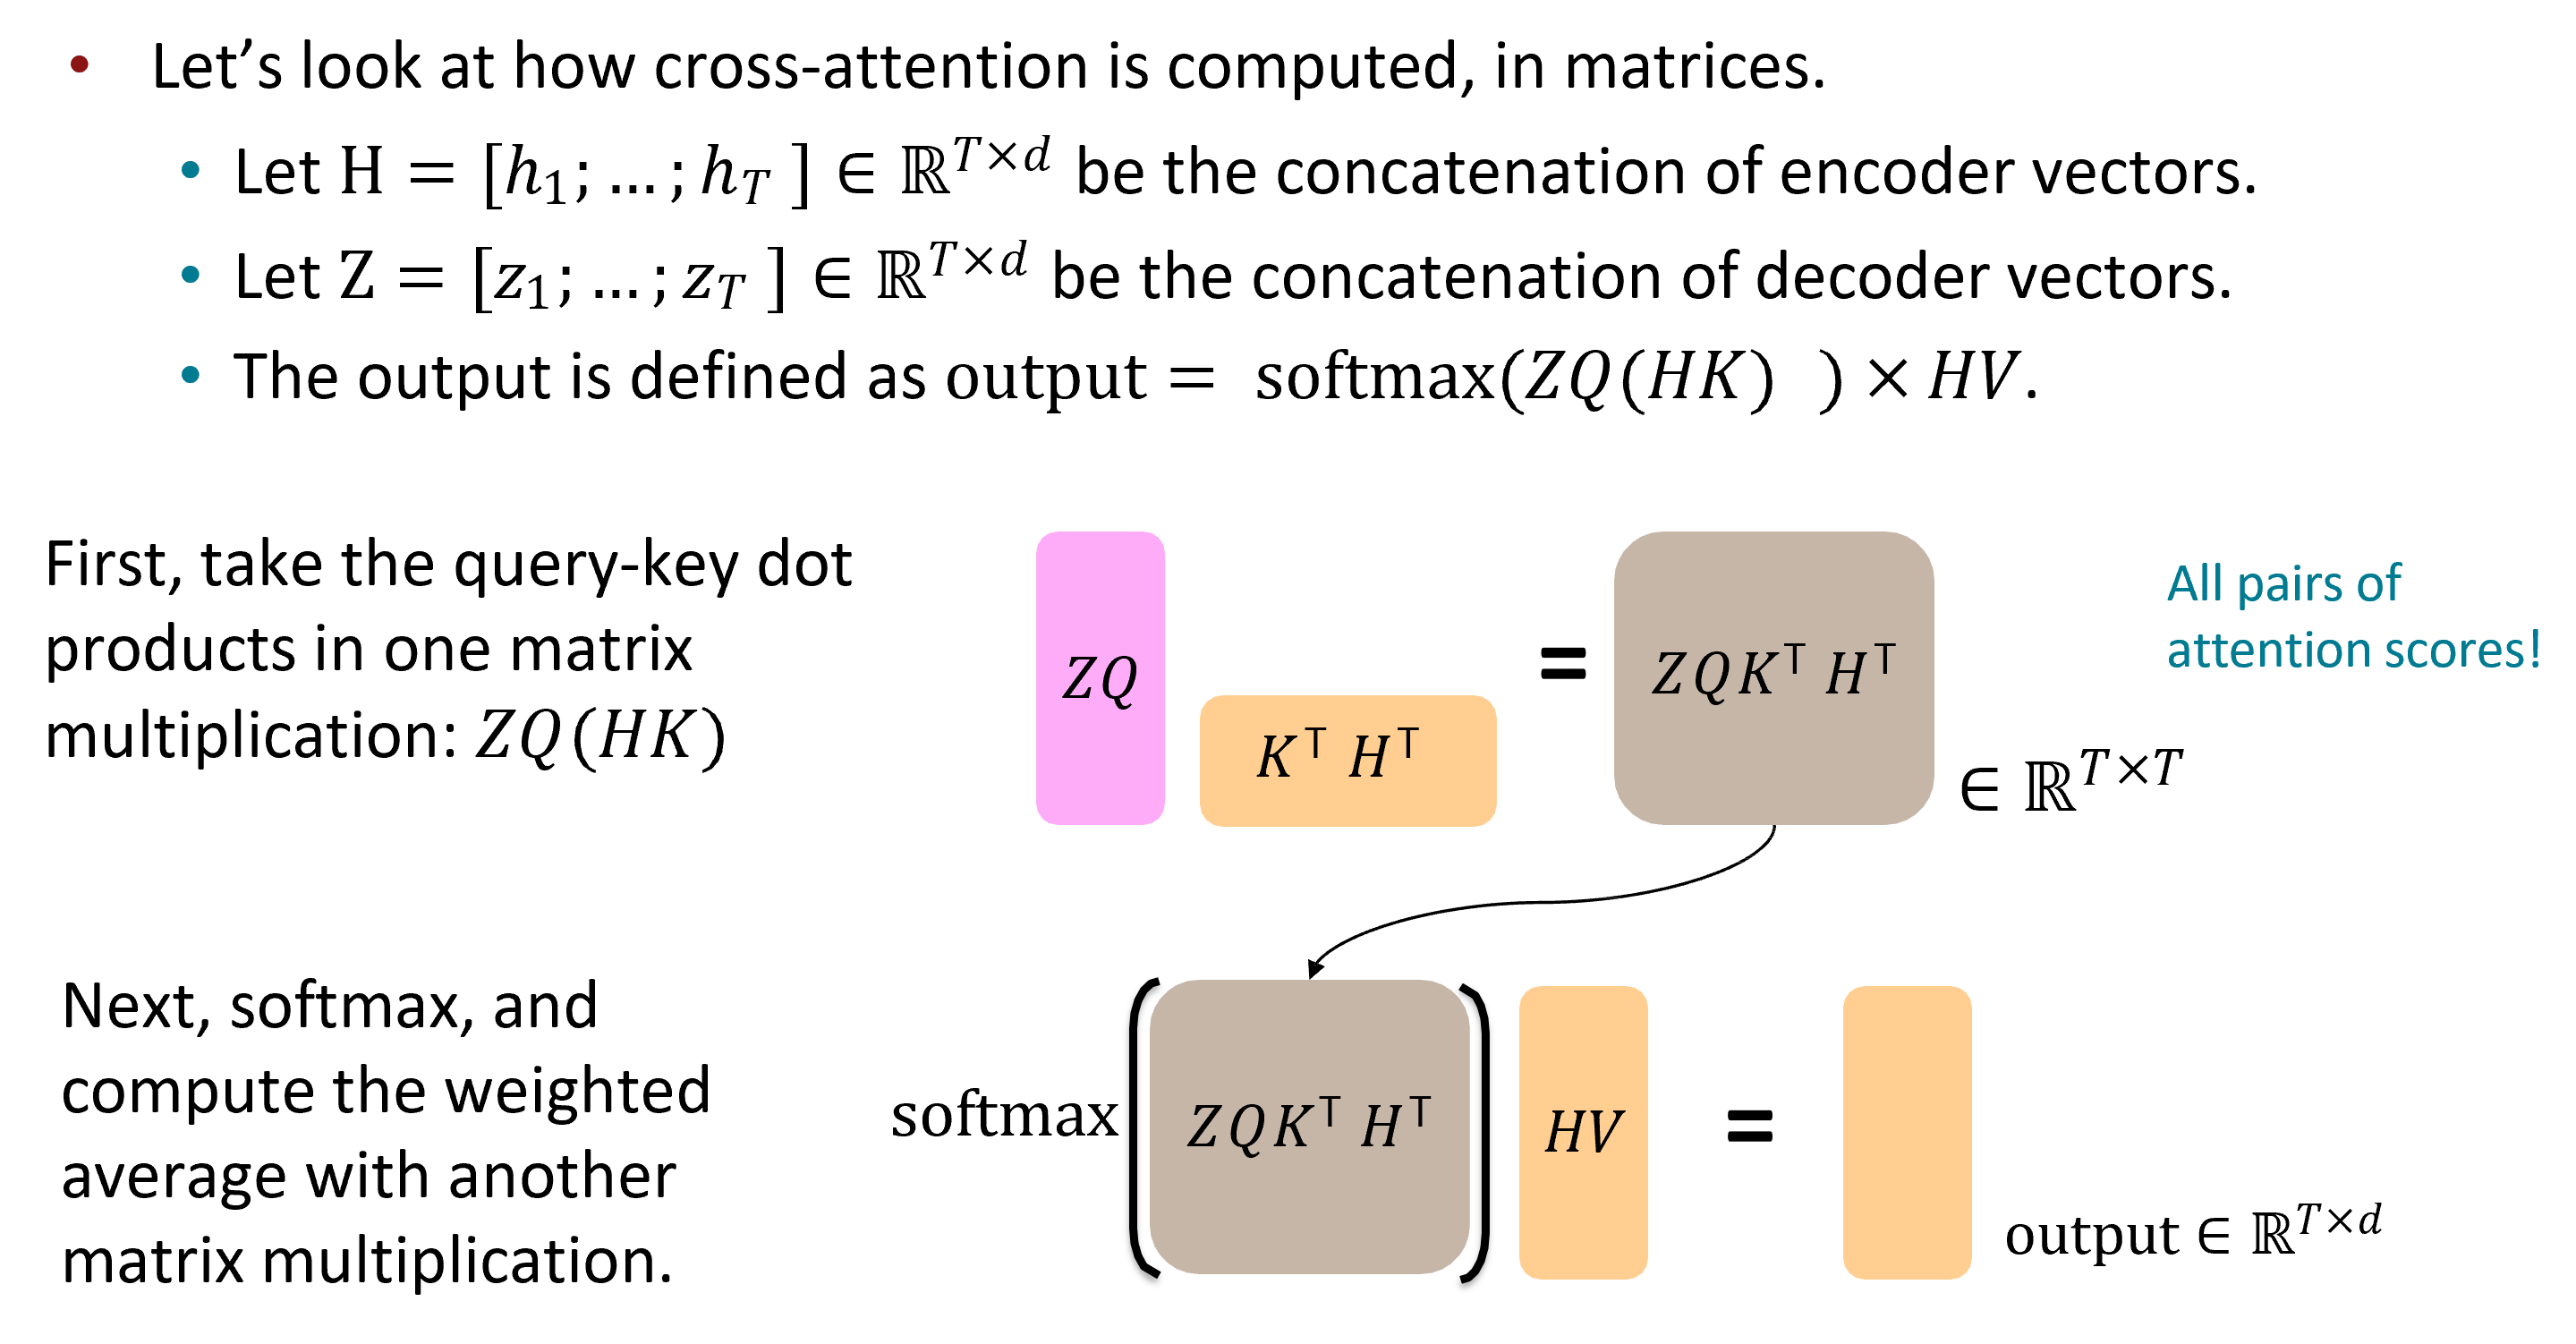
\includegraphics[width=\linewidth,keepaspectratio]{bert90}
			% \end{center}		
			
			% % {\tiny (Ref: John Hewitt)}

% \end{frame}

% %%%%%%%%%%%%%%%%%%%%%%%%%%%%%%%%%%%%%%%%%%%%%%%%%%%%%%%%%%%
% \begin{frame}[fragile]\frametitle{Results}
% Great Results with Transformers
			
			% \begin{center}
			% 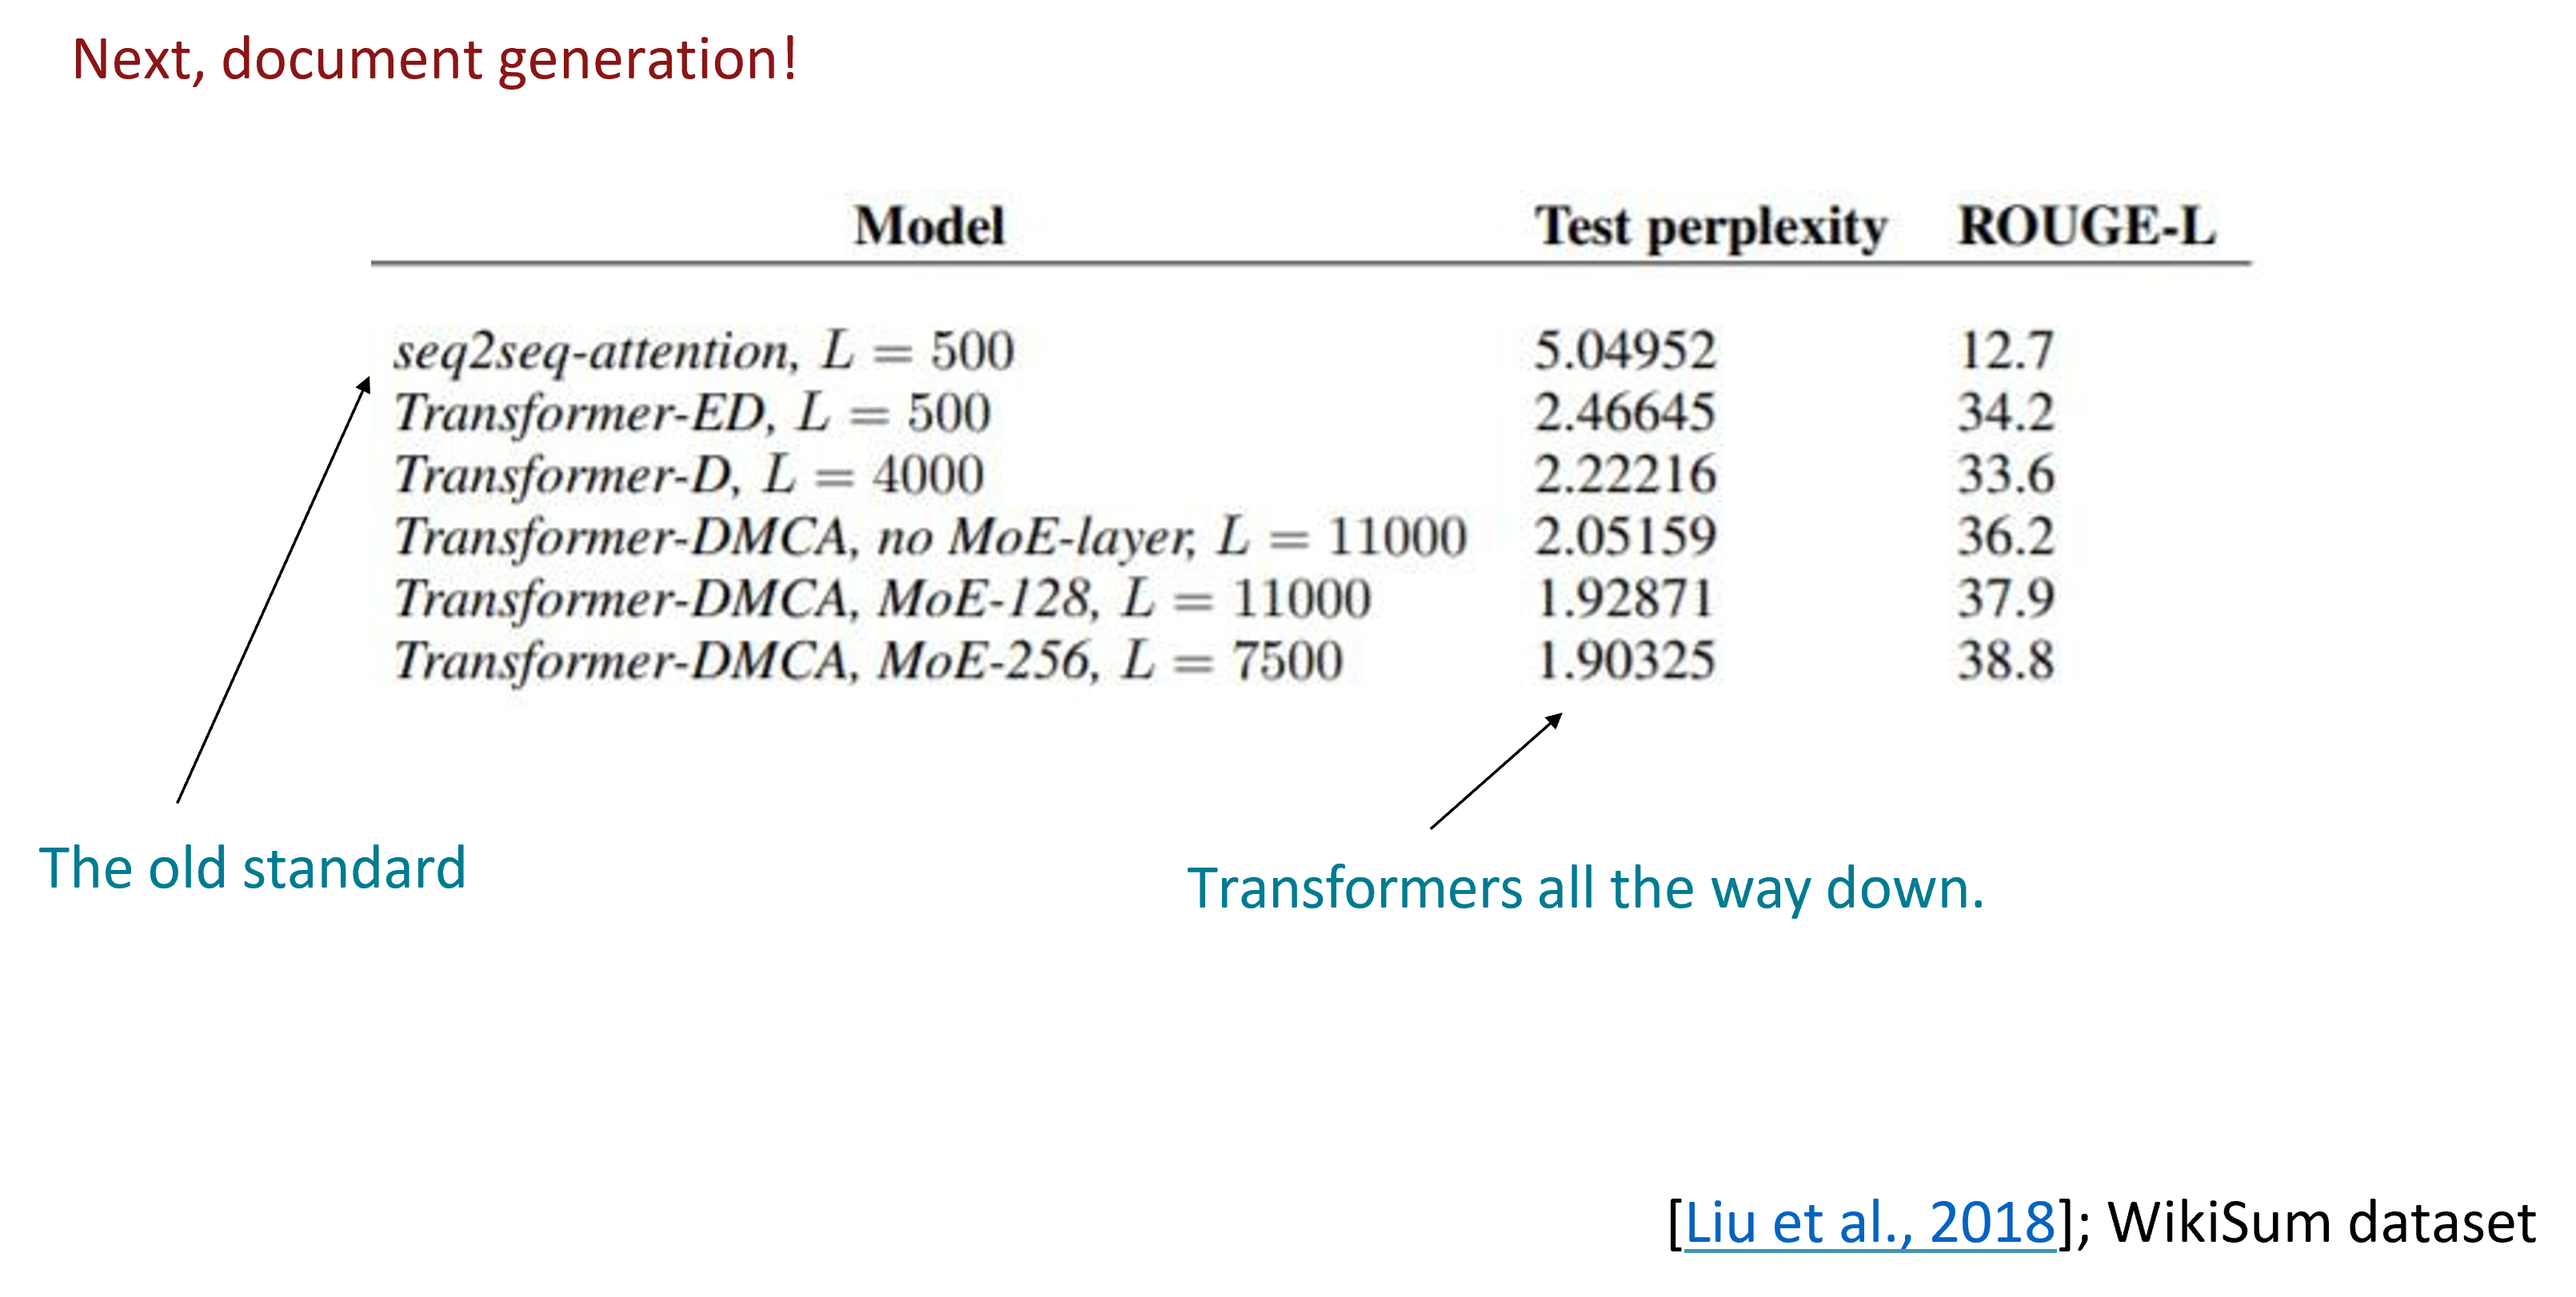
\includegraphics[width=\linewidth,keepaspectratio]{bert91}
			% \end{center}		
			
			% % {\tiny (Ref: John Hewitt)}

% \end{frame}

% %%%%%%%%%%%%%%%%%%%%%%%%%%%%%%%%%%%%%%%%%%%%%%%%%%%%%%%%%%%
% \begin{frame}[fragile]\frametitle{Issues}

% What would we like to fix about the Transformer?

      % \begin{itemize}
			% \item Quadratic compute in self-attention:
			      % \begin{itemize}
						% \item Computing all pairs of interactions means our computation grows quadratically with the sequence length!
						% \item For recurrent models, it only grew linearly!
						% \end{itemize}
			% \item Position representations:
			      % \begin{itemize}
						% \item Are simple absolute indices the best we can do to represent position?
						% \item Relative linear position attention [Shaw et al., 2018]
						% \item Dependency syntax-based position [Wang et al., 2019]			
						% \end{itemize}
			% \end{itemize}

			% % {\tiny (Ref: John Hewitt)}

% \end{frame}

% %%%%%%%%%%%%%%%%%%%%%%%%%%%%%%%%%%%%%%%%%%%%%%%%%%%%%%%%%%%
% \begin{frame}[fragile]\frametitle{Quadratic computation as function of seq. length}

			
			% \begin{center}
			% 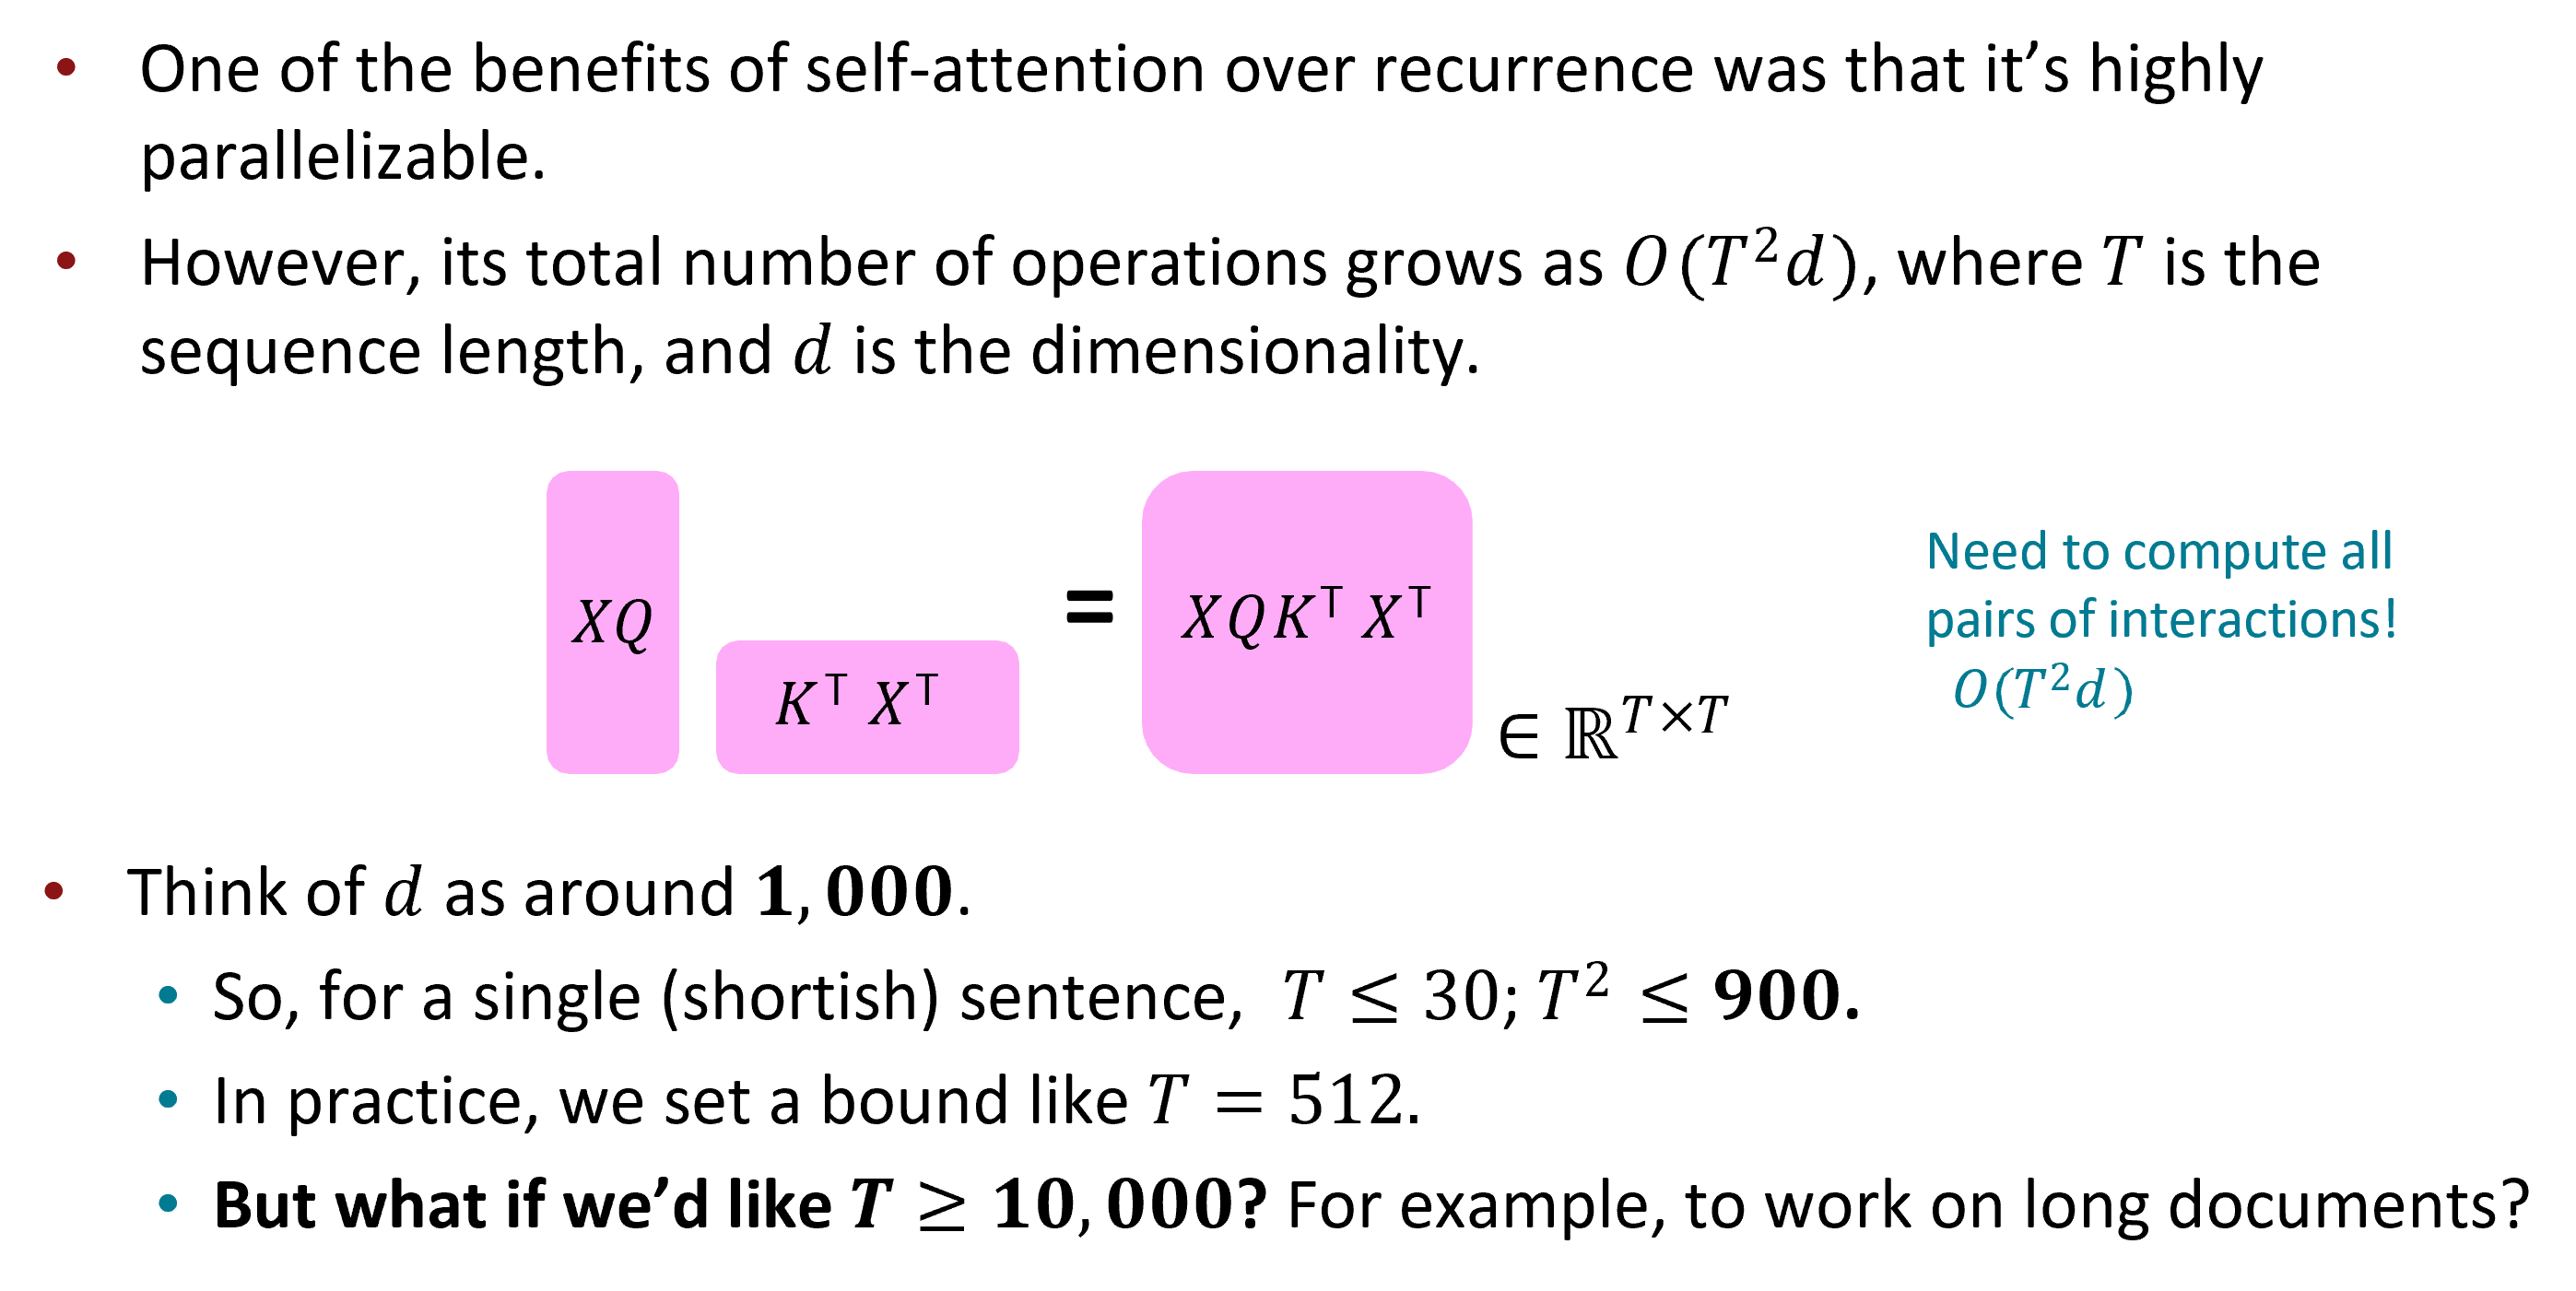
\includegraphics[width=\linewidth,keepaspectratio]{bert92}
			% \end{center}		
			
			% % {\tiny (Ref: John Hewitt)}

% \end{frame}

% %%%%%%%%%%%%%%%%%%%%%%%%%%%%%%%%%%%%%%%%%%%%%%%%%%%%%%%%%%%
% \begin{frame}[fragile]\frametitle{Recent work on improving on quadratic self-attention cost}

			
			% \begin{center}
			% 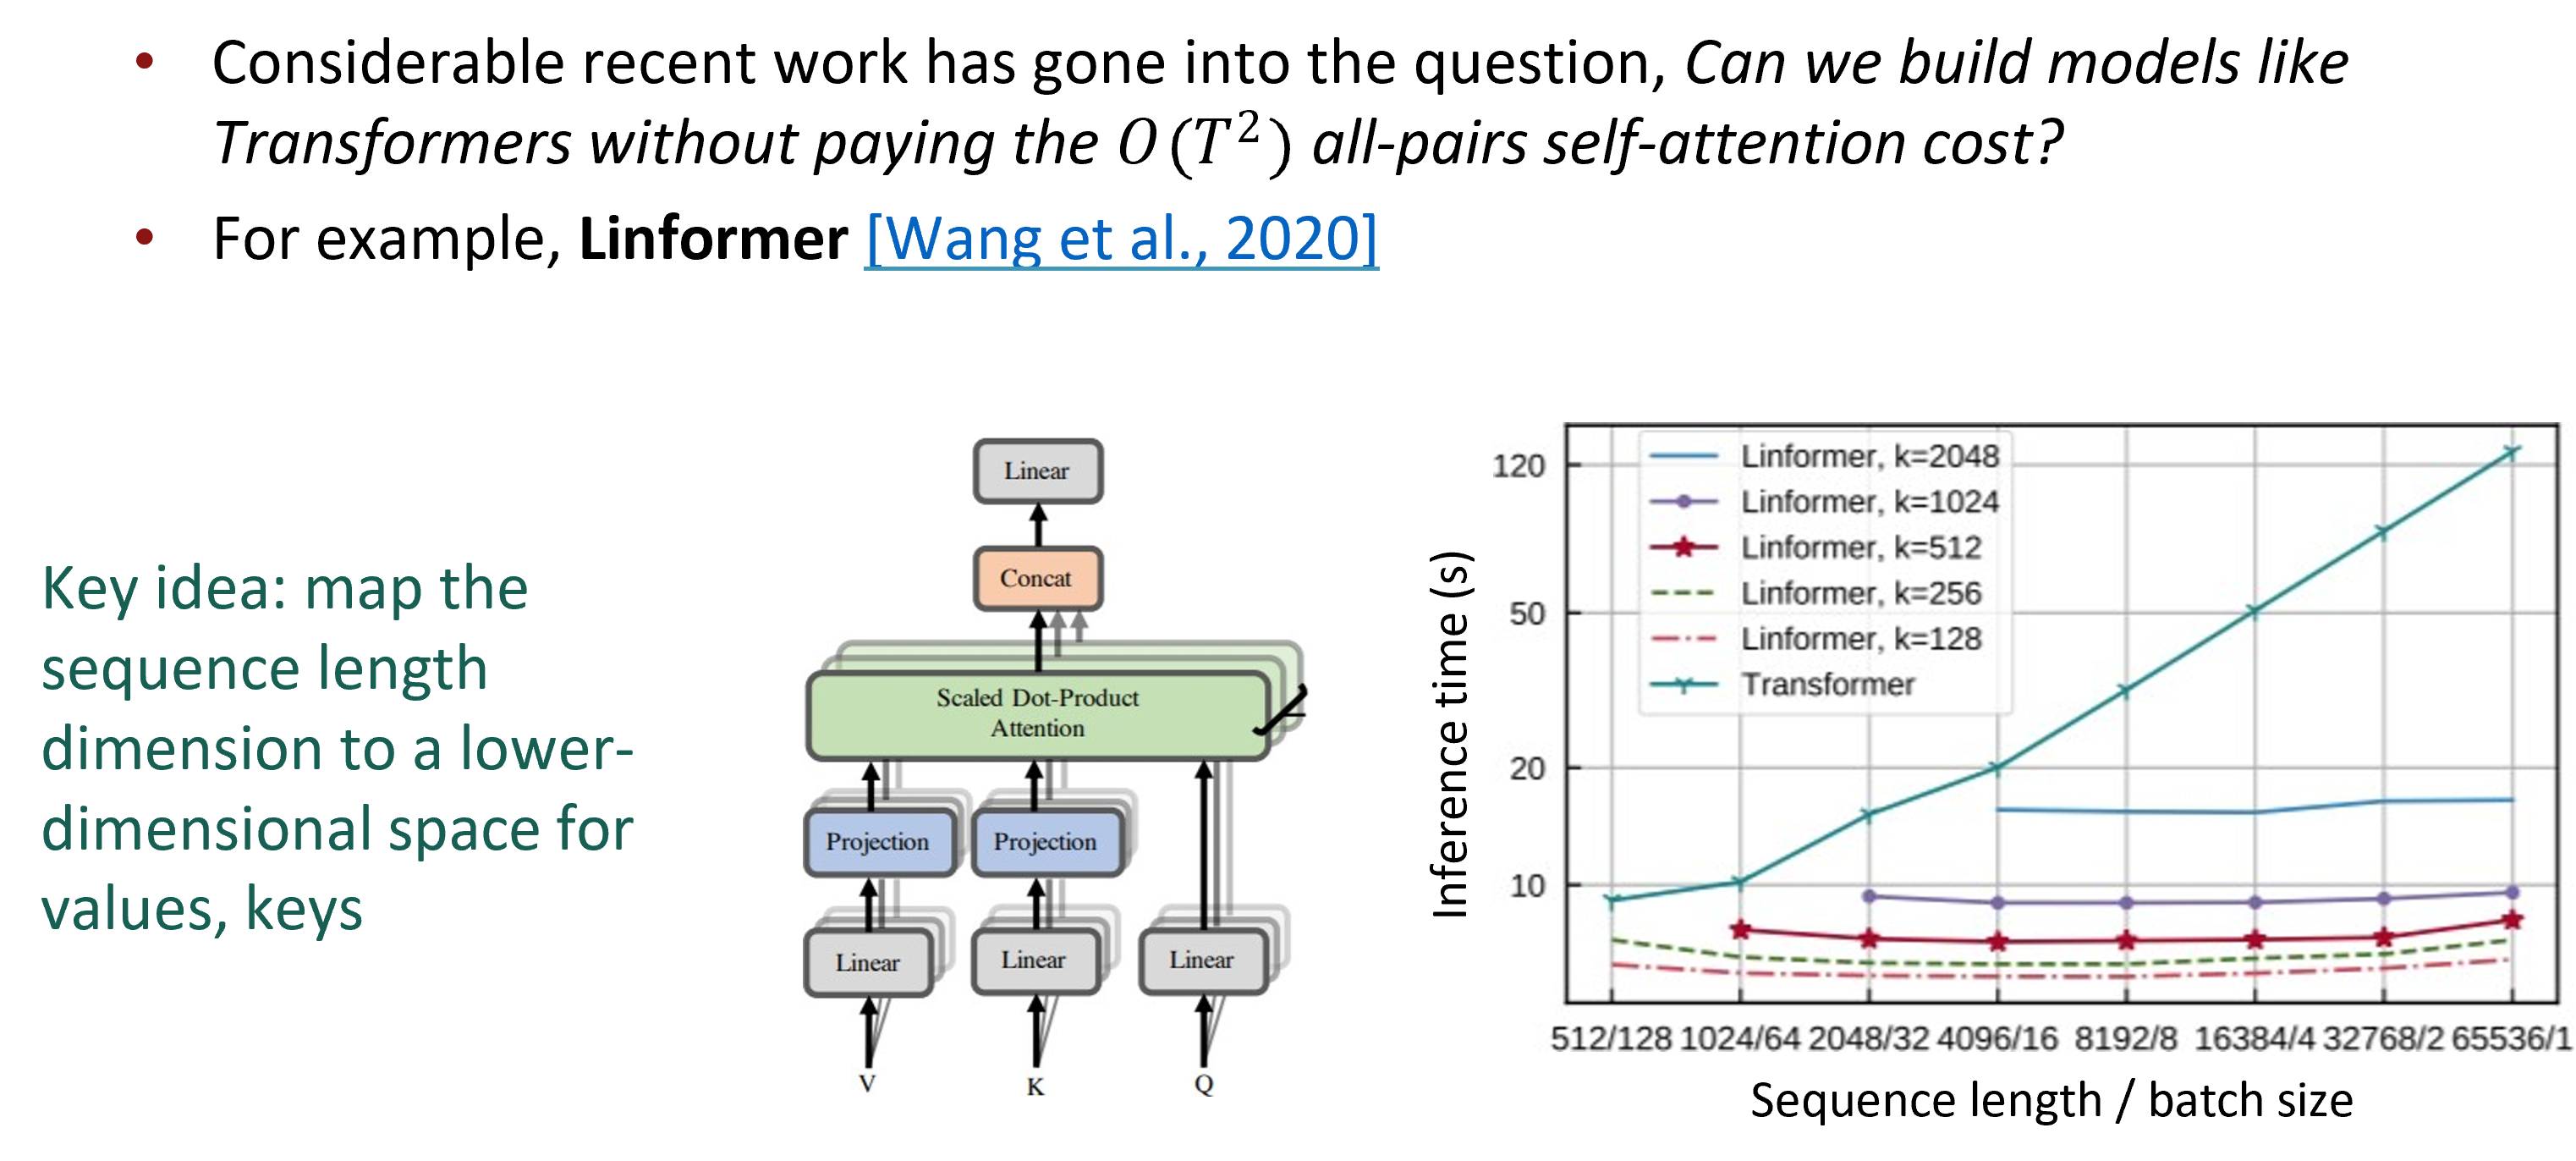
\includegraphics[width=\linewidth,keepaspectratio]{bert93}
			% \end{center}		
			
			% % {\tiny (Ref: John Hewitt)}

% \end{frame}

% %%%%%%%%%%%%%%%%%%%%%%%%%%%%%%%%%%%%%%%%%%%%%%%%%%%%%%%%%%%
% \begin{frame}[fragile]\frametitle{Recent work on improving on quadratic self-attention cost}

			
			% \begin{center}
			% 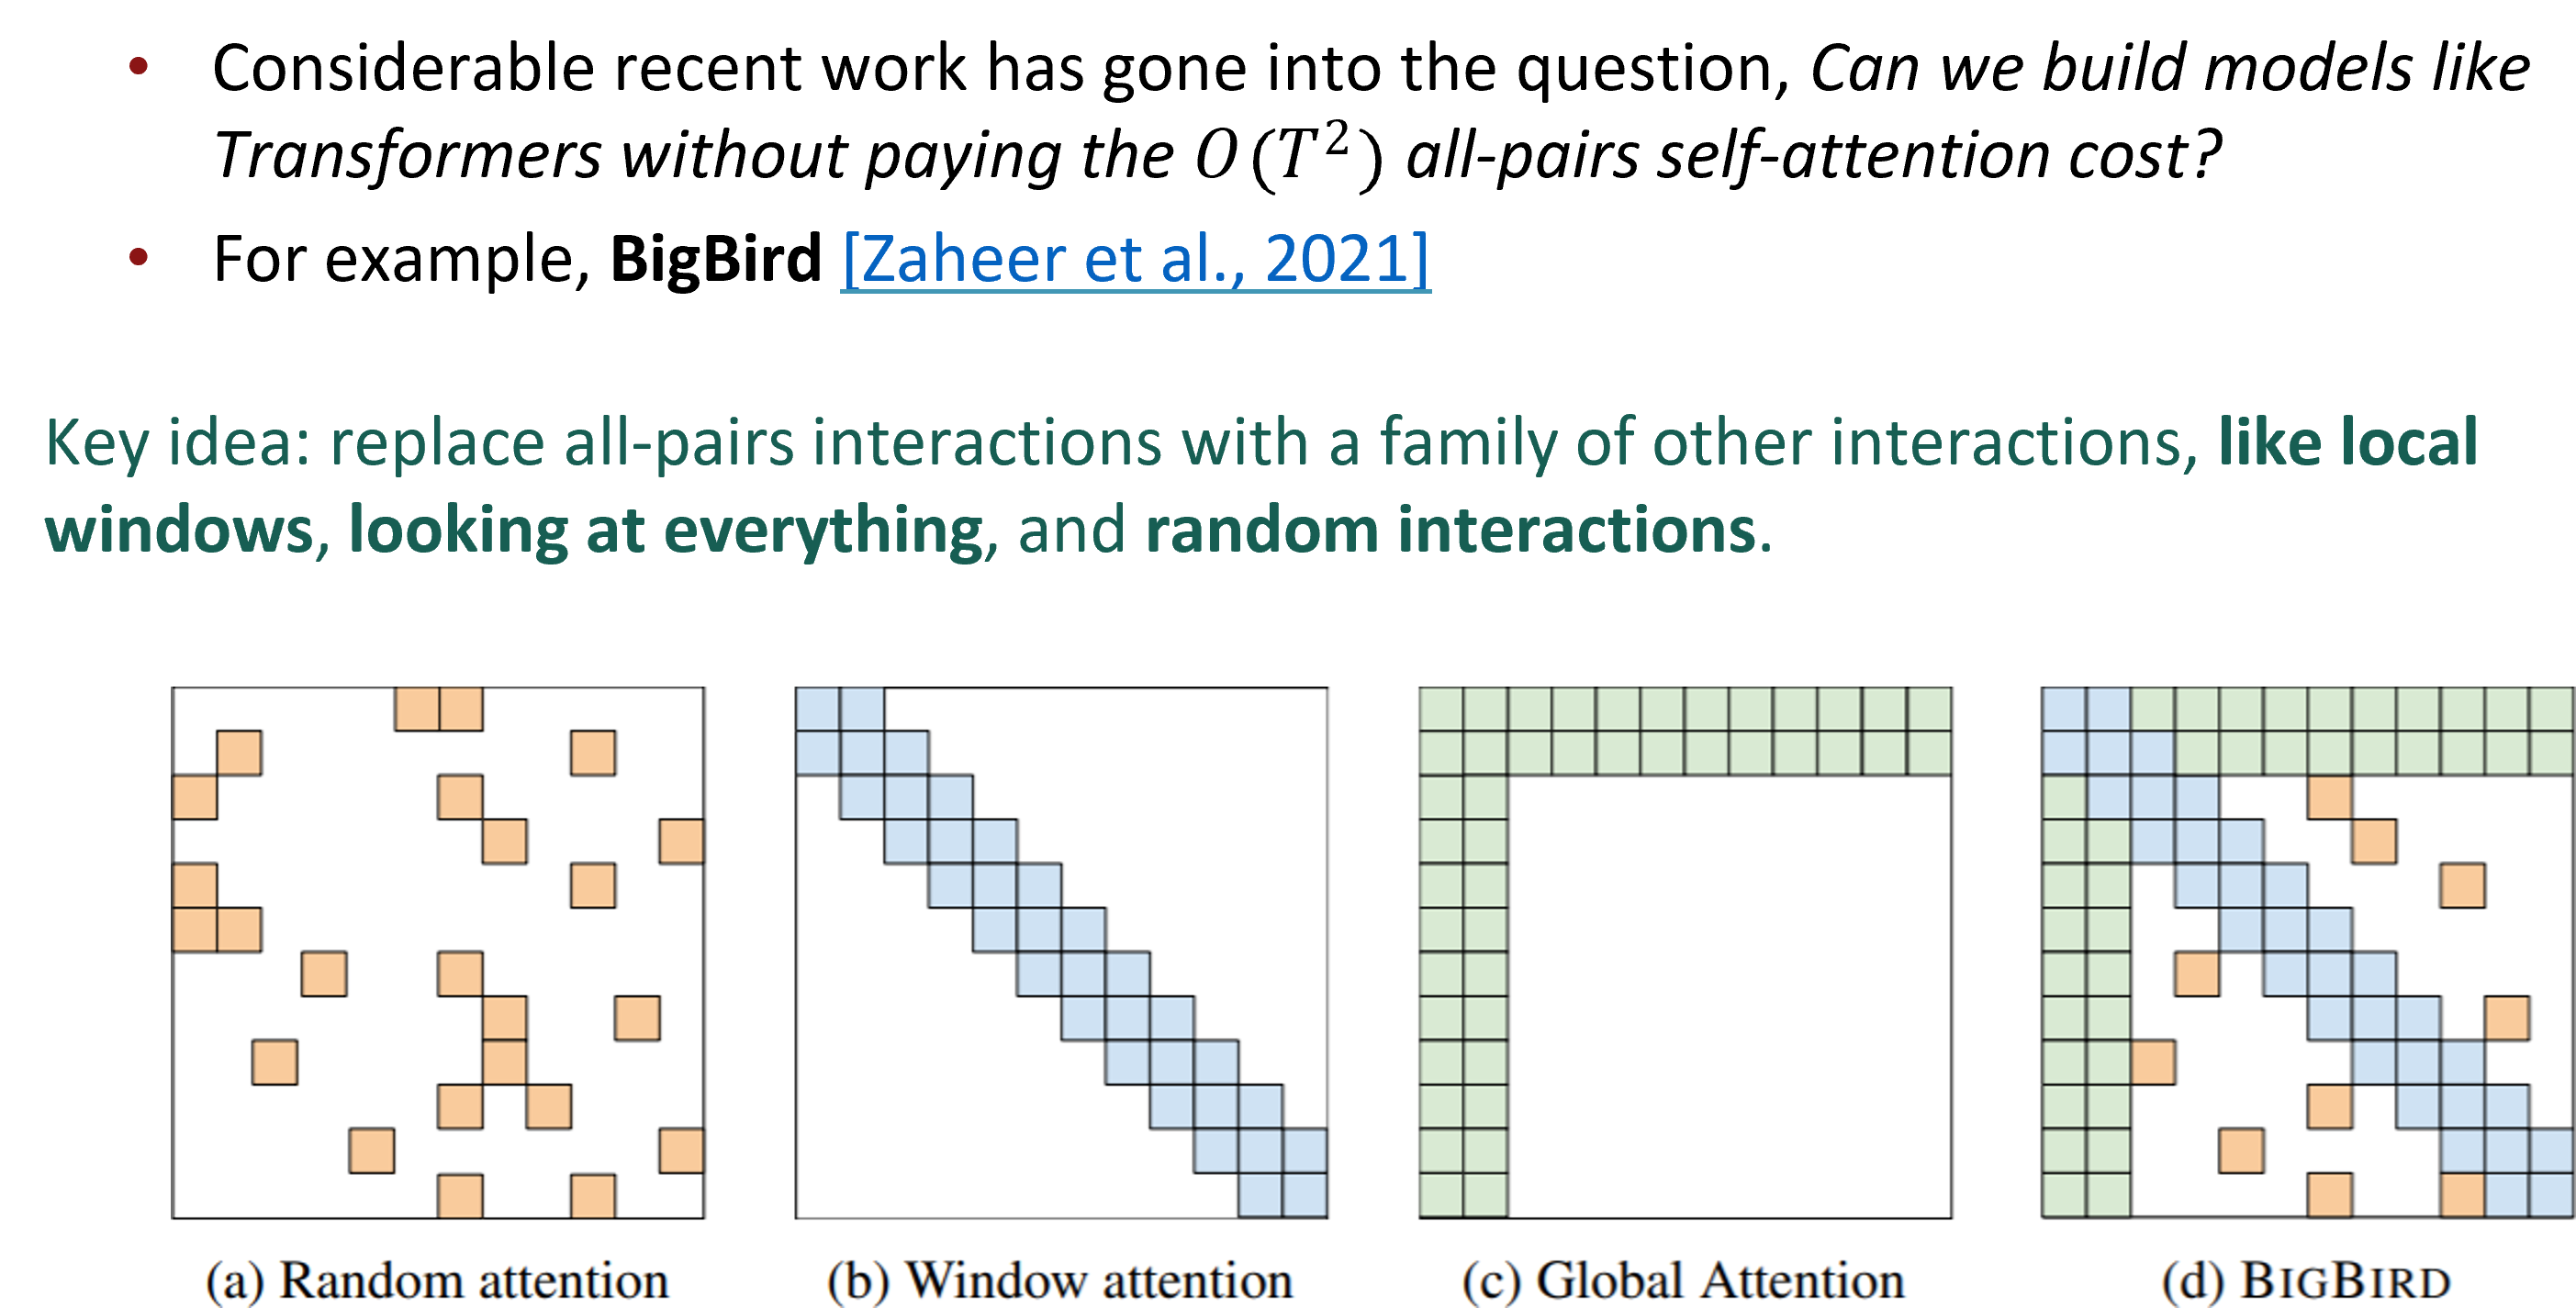
\includegraphics[width=\linewidth,keepaspectratio]{bert94}
			% \end{center}		
			
			% % {\tiny (Ref: John Hewitt)}

% \end{frame}

% %%%%%%%%%%%%%%%%%%%%%%%%%%%%%%%%%%%%%%%%%%%%%%%%%%%%%%%%%%%
% \begin{frame}[fragile]\frametitle{Recent work on improving on quadratic self-attention cost}

			
			% \begin{center}
			% 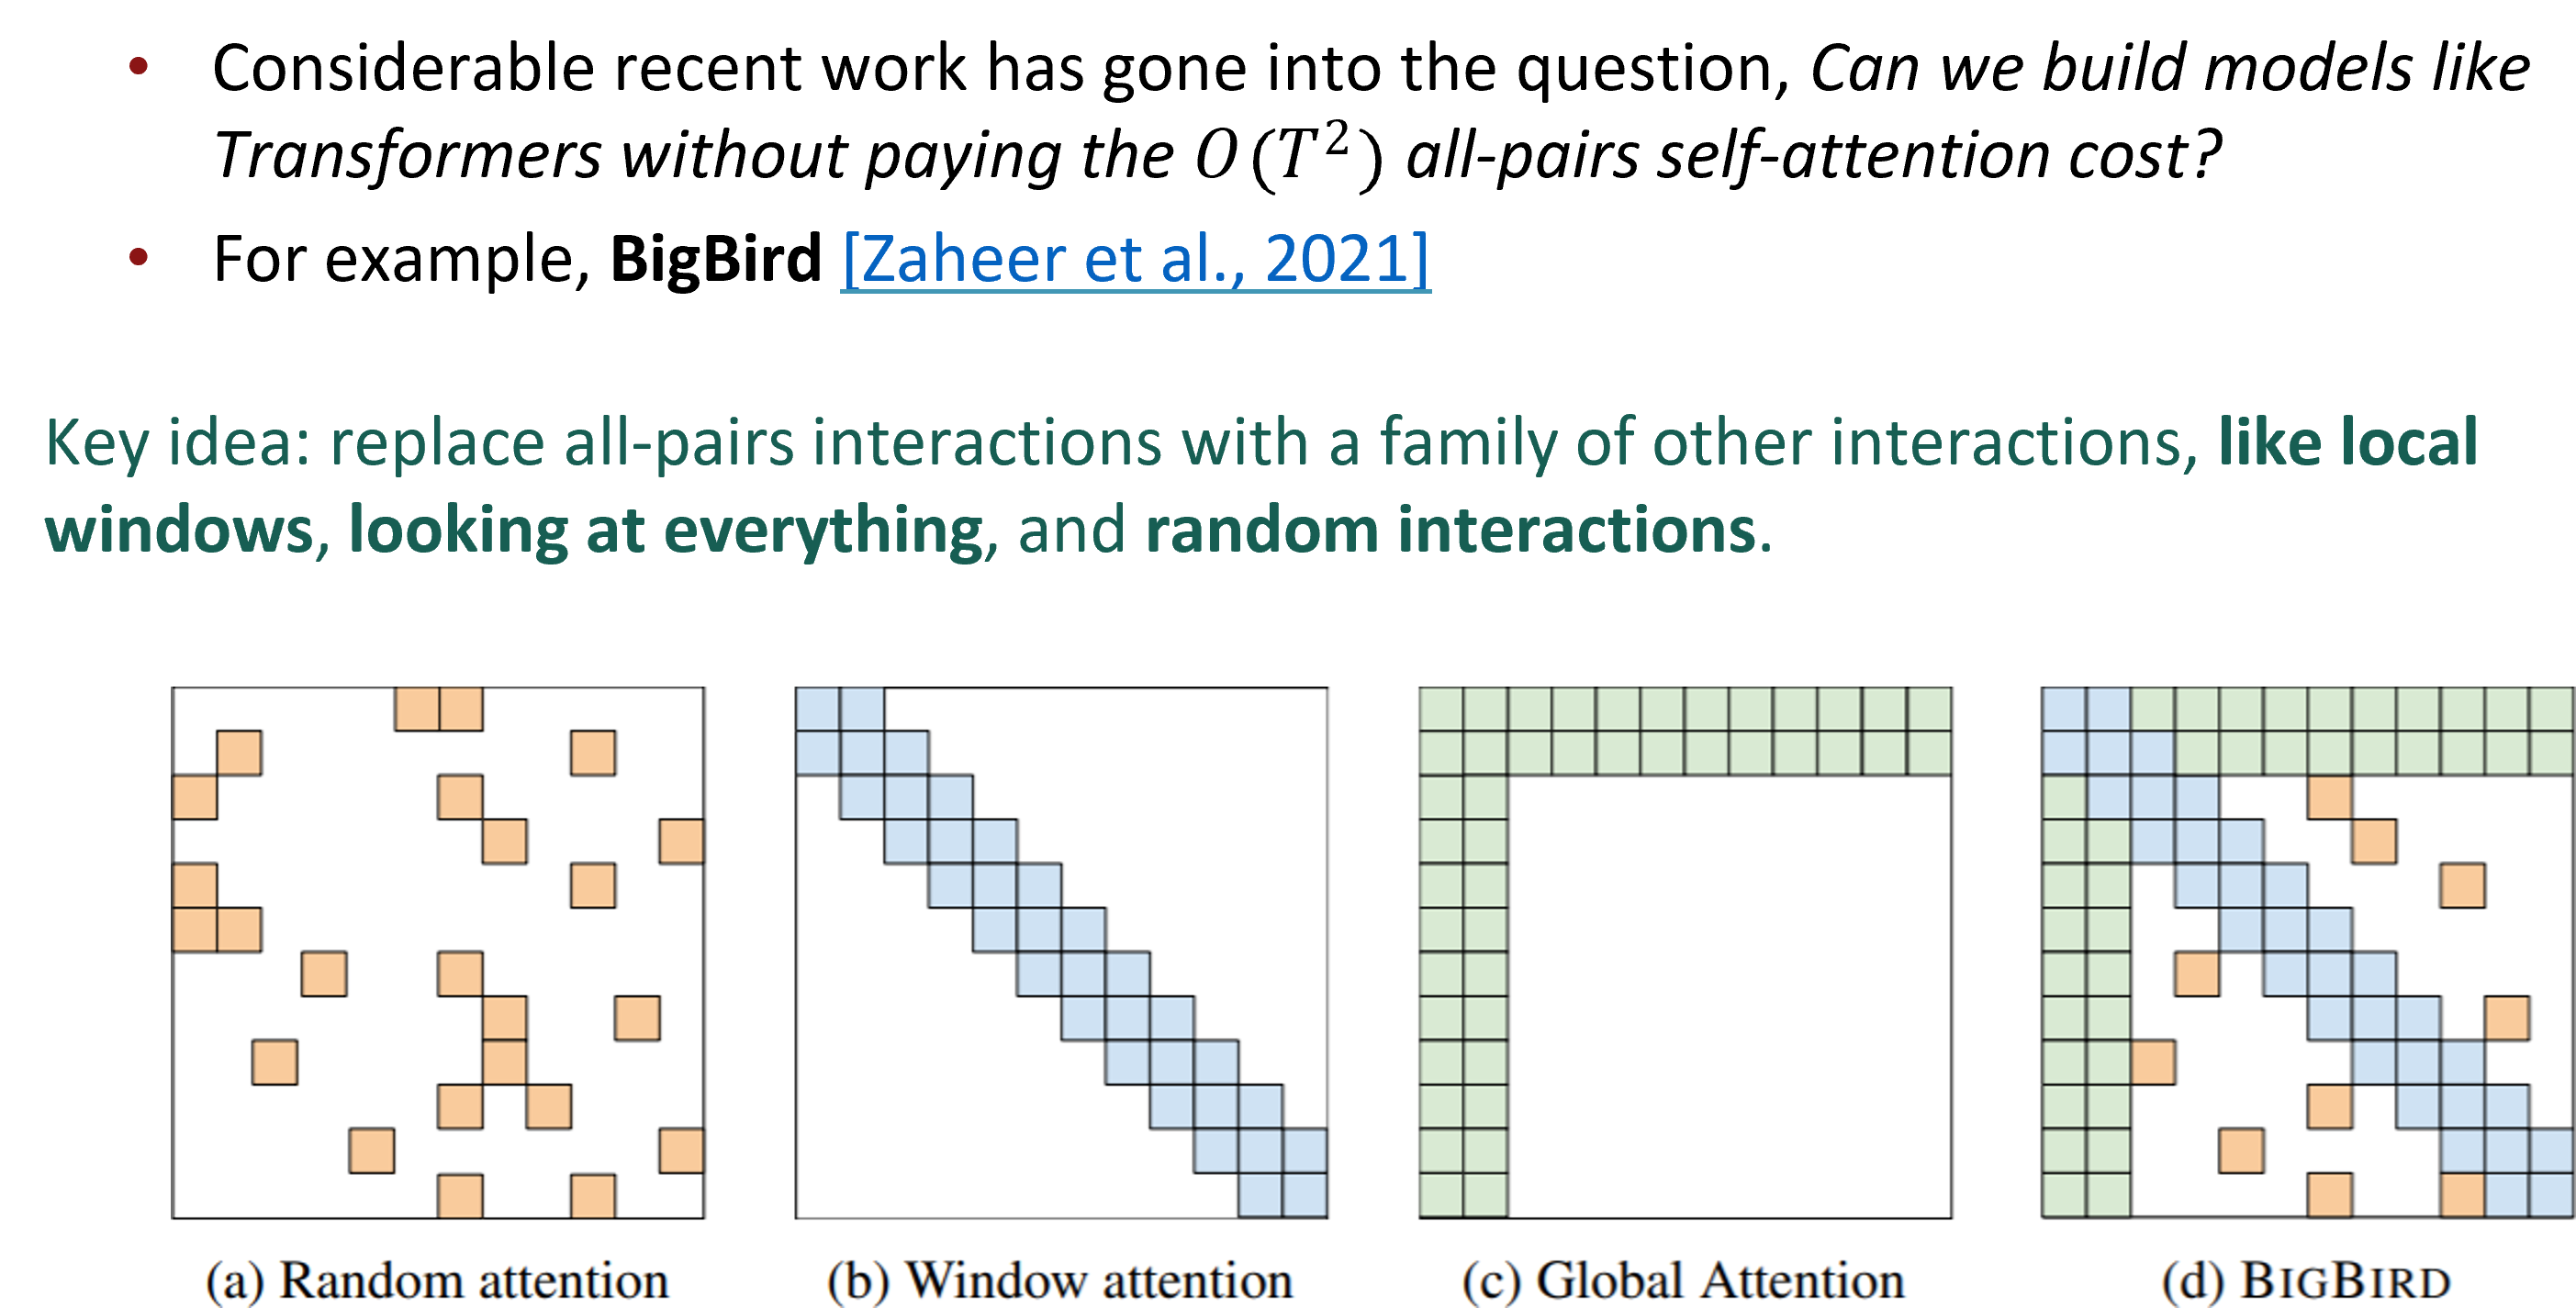
\includegraphics[width=\linewidth,keepaspectratio]{bert95}
			% \end{center}		
			
			% % {\tiny (Ref: John Hewitt)}

% \end{frame}

% %%%%%%%%%%%%%%%%%%%%%%%%%%%%%%%%%%%%%%%%%%%%%%%%%%%%%%%%%%%%%%%%%%%%%%%%%%%%%%%%%%
% \begin{frame}[fragile]\frametitle{}
% \begin{center}
% {\Large Pretraining models}
% \end{center}
% \end{frame}


% %%%%%%%%%%%%%%%%%%%%%%%%%%%%%%%%%%%%%%%%%%%%%%%%%%%%%%%%%%%
% \begin{frame}[fragile]\frametitle{Introduction}

			
			% \begin{center}
			% 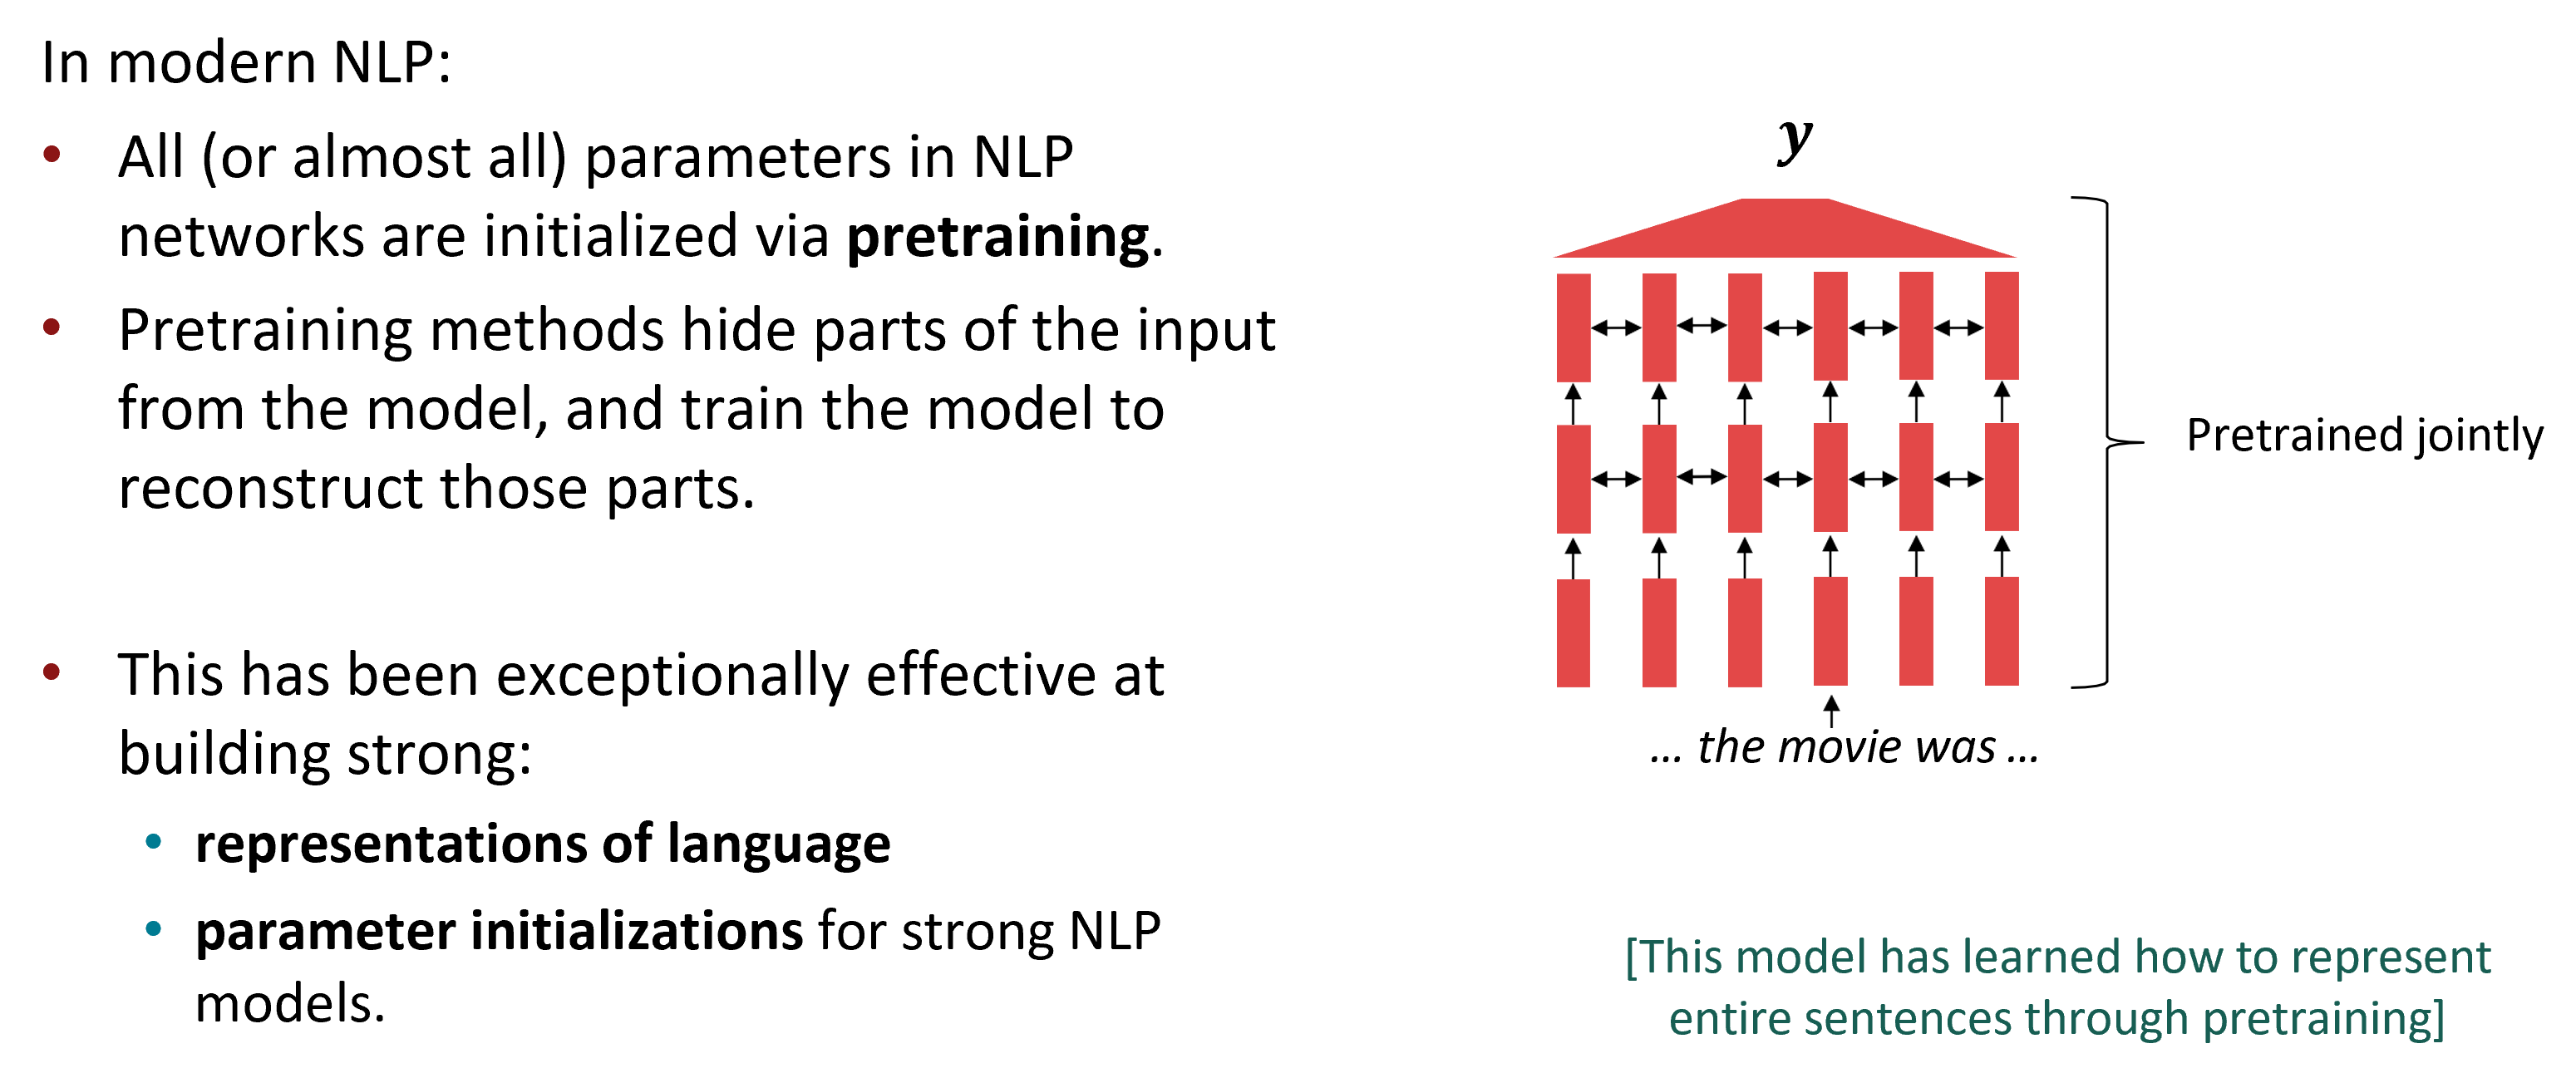
\includegraphics[width=\linewidth,keepaspectratio]{bert96}
			% \end{center}		
			
			% % {\tiny (Ref: John Hewitt)}

% \end{frame}

% %%%%%%%%%%%%%%%%%%%%%%%%%%%%%%%%%%%%%%%%%%%%%%%%%%%%%%%%%%%
% \begin{frame}[fragile]\frametitle{Pretraining models}
% Pretraining through language modeling [Dai and Le, 2015]
			
			% \begin{center}
			% 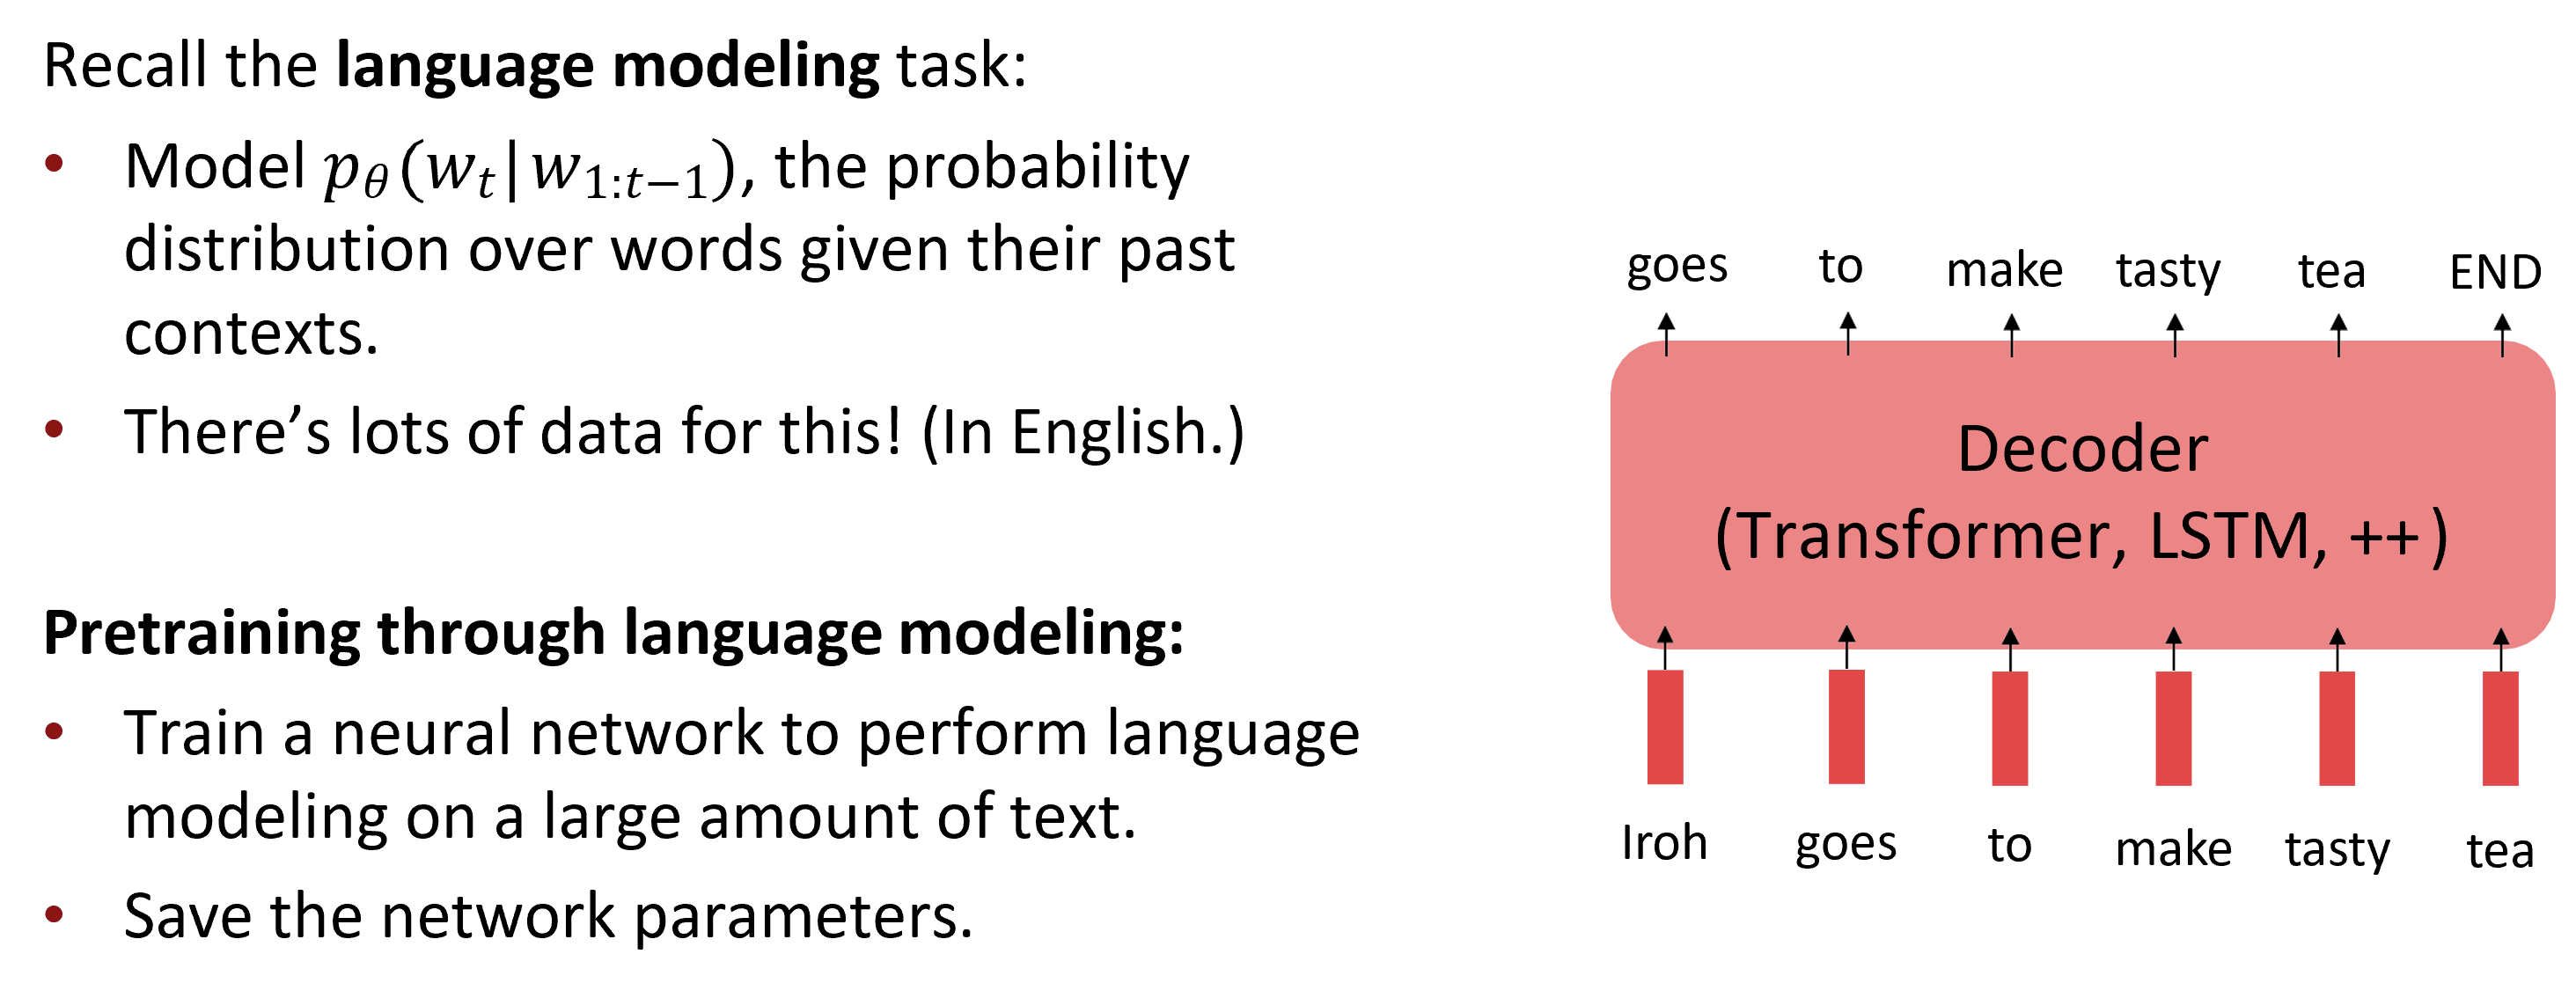
\includegraphics[width=\linewidth,keepaspectratio]{bert97}
			% \end{center}		
			
			% % {\tiny (Ref: John Hewitt)}

% \end{frame}

% %%%%%%%%%%%%%%%%%%%%%%%%%%%%%%%%%%%%%%%%%%%%%%%%%%%%%%%%%%%
% \begin{frame}[fragile]\frametitle{The Pretraining / Finetuning Paradigm}

			
			% \begin{center}
			% 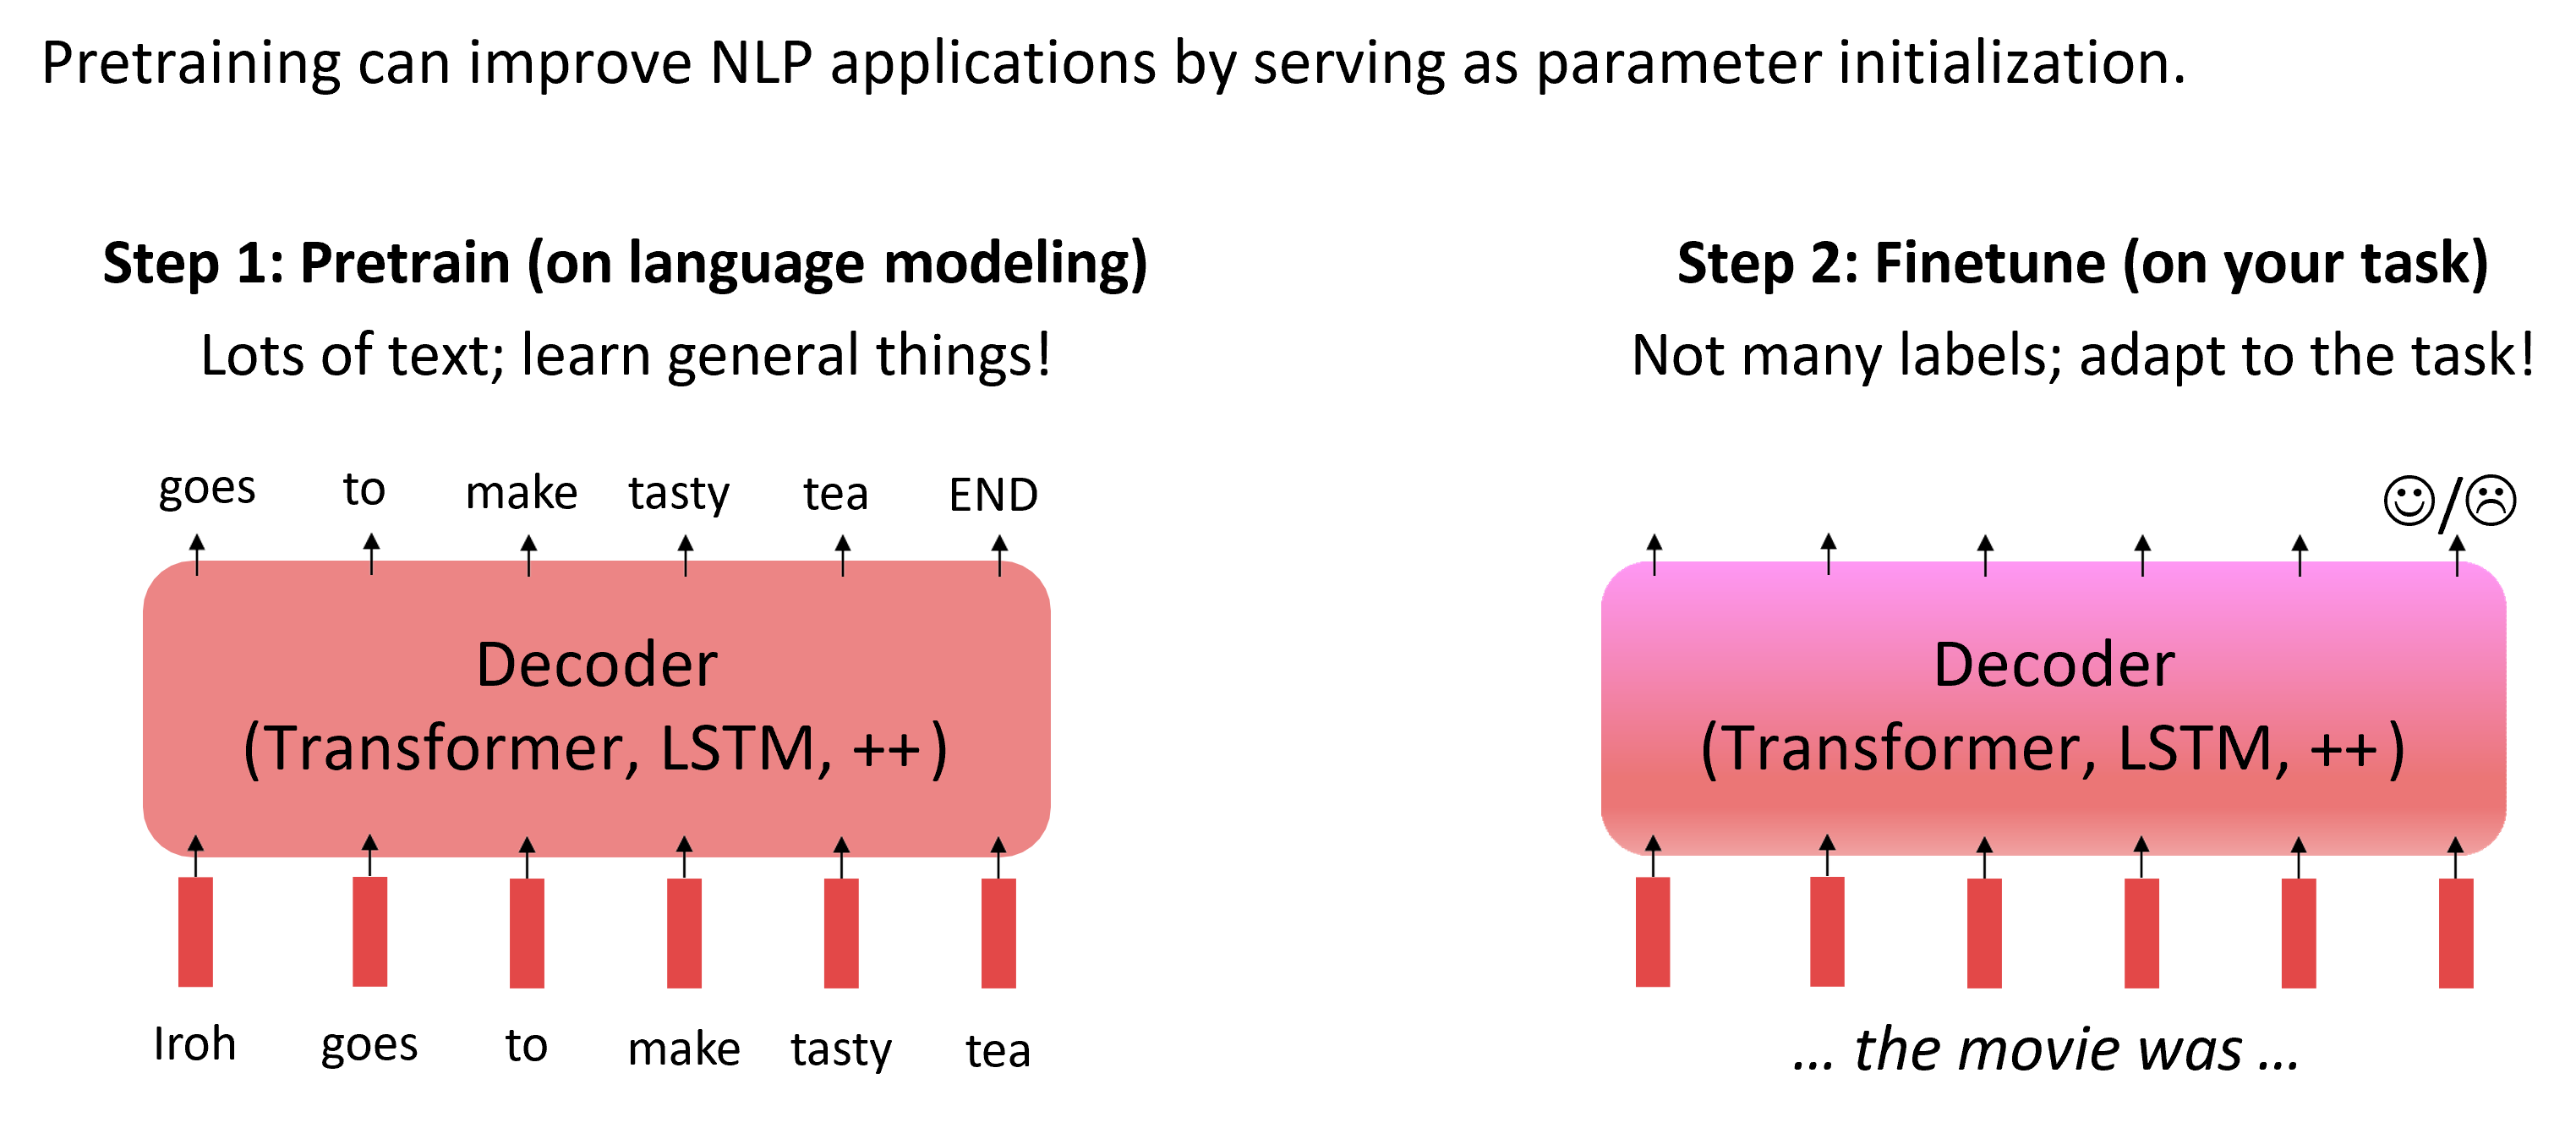
\includegraphics[width=\linewidth,keepaspectratio]{bert98}
			% \end{center}		
			
			% % {\tiny (Ref: John Hewitt)}

% \end{frame}

% % %%%%%%%%%%%%%%%%%%%%%%%%%%%%%%%%%%%%%%%%%%%%%%%%%%%%%%%%%%%
% % \begin{frame}[fragile]\frametitle{Capturing meaning via context}

% % Increasing evidence that pretrained models learn a wide variety of things about
% % the statistical properties of language:

      % % \begin{itemize}
			% % \item Stanford University is located in $--$, California. [Trivia]
			% % \item I put $--$ fork down on the table. [syntax]
			% % \item The woman walked across the street, checking for traffic over $--$ shoulder. [coreference]
			% % \item I went to the ocean to see the fish, turtles, seals, and $--$.	[lexical semantics/topic]
			% % \item Overall, the value I got from the two hours watching it was the sum total of the popcorn and the drink. The movie was $--$. [sentiment]
			% % \item Iroh went into the kitchen to make some tea. Standing next to Iroh, Zuko pondered his  destiny. Zuko left the $--$. [some reasoning – this is harder]
			% % \item I was thinking about the sequence that goes 1, 1, 2, 3, 5, 8, 13, 21, $--$[some basic arithmetic; they don’t learn the Fibonnaci sequence]
			% % \item Models also learn – and can exacerbate racism, sexism, all manner of bad biases.
			% % \item More on all this in the Interpretability lecture!

			% % \end{itemize}

			% % % {\tiny (Ref: John Hewitt)}

% % \end{frame}

% %%%%%%%%%%%%%%%%%%%%%%%%%%%%%%%%%%%%%%%%%%%%%%%%%%%%%%%%%%%
% \begin{frame}[fragile]\frametitle{Pretraining}

			% Pretraining for three types of architectures
			
			% \begin{center}
			% \includegraphics[width=\linewidth,keepaspectratio]{bert99}
			% \end{center}		
			
			% % {\tiny (Ref: John Hewitt)}

% \end{frame}

% %%%%%%%%%%%%%%%%%%%%%%%%%%%%%%%%%%%%%%%%%%%%%%%%%%%%%%%%%%%
% \begin{frame}[fragile]\frametitle{Pretraining}

			% Pretraining encoder-decoders: What pretraining objective to use?
			
			% \begin{center}
			% \includegraphics[width=\linewidth,keepaspectratio]{bert100}
			% \end{center}		
			
			% % {\tiny (Ref: John Hewitt)}

% \end{frame}

% %%%%%%%%%%%%%%%%%%%%%%%%%%%%%%%%%%%%%%%%%%%%%%%%%%%%%%%%%%%
% \begin{frame}[fragile]\frametitle{Pretraining}

			% Pretraining encoder-decoders: What pretraining objective to use?

			
			% \begin{center}
			% \includegraphics[width=\linewidth,keepaspectratio]{bert101}
			% \end{center}		
			
			% % {\tiny (Ref: John Hewitt)}

% \end{frame}


% %%%%%%%%%%%%%%%%%%%%%%%%%%%%%%%%%%%%%%%%%%%%%%%%%%%%%%%%%%%
% \begin{frame}[fragile]\frametitle{Pretraining decoders}


			% \begin{center}
			% \includegraphics[width=\linewidth,keepaspectratio]{bert104}
			% \end{center}		
			
			% % {\tiny (Ref: John Hewitt)}

% \end{frame}

% %%%%%%%%%%%%%%%%%%%%%%%%%%%%%%%%%%%%%%%%%%%%%%%%%%%%%%%%%%%
% \begin{frame}[fragile]\frametitle{Pretraining decoders}


			% \begin{center}
			% \includegraphics[width=\linewidth,keepaspectratio]{bert105}
			% \end{center}		
			
			% % {\tiny (Ref: John Hewitt)}

% \end{frame}

% % %%%%%%%%%%%%%%%%%%%%%%%%%%%%%%%%%%%%%%%%%%%%%%%%%%%%%%%%%%%
% % \begin{frame}[fragile]\frametitle{Aside: Word structure and subword models}

			% % \begin{center}
			% % \includegraphics[width=\linewidth,keepaspectratio]{bert109}
			% % \end{center}		
			
			% % % {\tiny (Ref: John Hewitt)}

% % \end{frame}

% % %%%%%%%%%%%%%%%%%%%%%%%%%%%%%%%%%%%%%%%%%%%%%%%%%%%%%%%%%%%
% % \begin{frame}[fragile]\frametitle{Aside: Word structure and subword models}

			% % \begin{center}
			% % \includegraphics[width=\linewidth,keepaspectratio]{bert110}
			% % \end{center}		
			
			% % % {\tiny (Ref: John Hewitt)}

% % \end{frame}


% % %%%%%%%%%%%%%%%%%%%%%%%%%%%%%%%%%%%%%%%%%%%%%%%%%%%%%%%%%%%
% % \begin{frame}[fragile]\frametitle{Aside: The byte-pair encoding algorithm}

			% % \begin{center}
			% % \includegraphics[width=\linewidth,keepaspectratio]{bert111}
			% % \end{center}		
			
			% % % {\tiny (Ref: John Hewitt)}

% % \end{frame}

% % %%%%%%%%%%%%%%%%%%%%%%%%%%%%%%%%%%%%%%%%%%%%%%%%%%%%%%%%%%%
% % \begin{frame}[fragile]\frametitle{Aside: Word structure and subword models}

			% % \begin{center}
			% % \includegraphics[width=\linewidth,keepaspectratio]{bert112}
			% % \end{center}		
			
			% % % {\tiny (Ref: John Hewitt)}

% % \end{frame}

% %%%%%%%%%%%%%%%%%%%%%%%%%%%%%%%%%%%%%%%%%%%%%%%%%%%%%%%%%%%%%%%%%%%%%%%%%%%%%%%%%%
% \begin{frame}[fragile]\frametitle{}
% \begin{center}
% {\Large GPT}
% \end{center}
% \end{frame}


% %%%%%%%%%%%%%%%%%%%%%%%%%%%%%%%%%%%%%%%%%%%%%%%%%%%%%%%%%%%
% \begin{frame}[fragile]\frametitle{Generative Pretrained Transformer (GPT)}

% [Radford et al., 2018]

% 2018’s GPT was a big success in pretraining a decoder!


      % \begin{itemize}
			% \item Transformer decoder with 12 layers.
			% \item 768-dimensional hidden states, 3072-dimensional feed-forward hidden layers.
			% \item Byte-pair encoding with 40,000 merges
			% \item Trained on BooksCorpus: over 7000 unique books.
			% \item Contains long spans of contiguous text, for learning long-distance dependencies.
			% \item The acronym ``GPT'' never showed up in the original paper; it could stand for
			% \item ``Generative PreTraining'' or ``Generative Pretrained Transformer''
			% \end{itemize}

			
			% % {\tiny (Ref: John Hewitt)}

% \end{frame}

% %%%%%%%%%%%%%%%%%%%%%%%%%%%%%%%%%%%%%%%%%%%%%%%%%%%%%%%%%%%
% \begin{frame}[fragile]\frametitle{GPT}

			% \begin{center}
			% \includegraphics[width=\linewidth,keepaspectratio]{bert106}
			% \end{center}		
			
			% % {\tiny (Ref: John Hewitt)}

% \end{frame}

% %%%%%%%%%%%%%%%%%%%%%%%%%%%%%%%%%%%%%%%%%%%%%%%%%%%%%%%%%%%
% \begin{frame}[fragile]\frametitle{GPT}

			% \begin{center}
			% \includegraphics[width=\linewidth,keepaspectratio]{bert107}
			% \end{center}		
			
			% % {\tiny (Ref: John Hewitt)}

% \end{frame}

% %%%%%%%%%%%%%%%%%%%%%%%%%%%%%%%%%%%%%%%%%%%%%%%%%%%%%%%%%%%
% \begin{frame}[fragile]\frametitle{GPT}

			% \begin{center}
			% \includegraphics[width=\linewidth,keepaspectratio]{bert108}
			% \end{center}		
			
			% % {\tiny (Ref: John Hewitt)}

% \end{frame}



% %%%%%%%%%%%%%%%%%%%%%%%%%%%%%%%%%%%%%%%%%%%%%%%%%%%%%%%%%%%
% \begin{frame}[fragile]\frametitle{GPT-3, in-context learning, very large models}


      % \begin{itemize}
			% \item So far, we’ve interacted with pretrained models in two ways:
			      % \begin{itemize}
						% \item Sample from the distributions they define (maybe providing a prompt)
						% \item Fine-tune them on a task we care about, and take their predictions.
						% \end{itemize}
			% \item Very large language models seem to perform some kind of learning without gradient  steps simply from examples you provide within their contexts.
			% \item GPT-3 is the canonical example of this. The largest T5 model had 11 billion parameters.
			% \item GPT-3 has 175 billion parameters.

			% \end{itemize}

			% % {\tiny (Ref: John Hewitt)}

% \end{frame}

% %%%%%%%%%%%%%%%%%%%%%%%%%%%%%%%%%%%%%%%%%%%%%%%%%%%%%%%%%%%
% \begin{frame}[fragile]\frametitle{GPT-3, in-context learning, very large models}


      % \begin{itemize}
			% \item Very large language models seem to perform some kind of learning without gradient  steps simply from examples you provide within their contexts.
			% \item The in-context examples seem to specify the task to be performed, and the conditional  distribution mocks performing the task to a certain extent.
			% \item Input (prefix within a single Transformer decoder context):
			% \end{itemize}

			% \begin{center}
			% \includegraphics[width=0.4\linewidth,keepaspectratio]{bert102}
			% \end{center}		
			
			% % {\tiny (Ref: John Hewitt)}

% \end{frame}

% %%%%%%%%%%%%%%%%%%%%%%%%%%%%%%%%%%%%%%%%%%%%%%%%%%%%%%%%%%%
% \begin{frame}[fragile]\frametitle{GPT-3, in-context learning, very large models}


			% \begin{center}
			% \includegraphics[width=\linewidth,keepaspectratio]{bert103}
			% \end{center}		
			
			% % {\tiny (Ref: John Hewitt)}

% \end{frame}


% \section[Concepts]{Concepts}
% %%%%%%%%%%%%%%%%%%%%%%%%%%%%%%%%%%%%%%%%%%%%%%%%%%%%%%%%%%%%%%%%%%%%%%%%%%%%%%%%%%
\begin{frame}[fragile]\frametitle{}
\begin{center}
{\Large BERT Concepts}
\end{center}
\end{frame}

%%%%%%%%%%%%%%%%%%%%%%%%%%%%%%%%%%%%%%%%%%%%%%%%%%%%%%%%%%%
\begin{frame}[fragile]\frametitle{Why BERT?}

BERT is the first, deeply bidirectional, unsupervised language representation, pre-trained using only a plain text corpus

			\begin{center}
			\includegraphics[width=\linewidth,keepaspectratio]{bert113}
			\end{center}		
			

\end{frame}

%%%%%%%%%%%%%%%%%%%%%%%%%%%%%%%%%%%%%%%%%%%%%%%%%%%%%%%%%%%
\begin{frame}[fragile]\frametitle{What is BERT?}


			\begin{center}
Bert stands for Bidirectional Encoder Representations from Transformers. It’s google’s new techniques for NLP pre-training language representation. Which means now machine learning communities can use Bert models that have been training already on a large number of words, for NLP models to do a wide variety of tasks such as Question Answering tasks, Named Entity Recognition (NER), and Classification like sentiment analysis.
			\end{center}		
			

\end{frame}

%%%%%%%%%%%%%%%%%%%%%%%%%%%%%%%%%%%%%%%%%%%%%%%%%%%%%%%%%%%
\begin{frame}[fragile]\frametitle{}

\begin{columns}
    \begin{column}[T]{0.5\linewidth}
			\begin{center}
			\includegraphics[width=0.8\linewidth,keepaspectratio]{bert114}
			\end{center}		
		\end{column}
    \begin{column}[T]{0.5\linewidth}
In Bert paper, they present two types of Bert models one is the Bert Base and the other is Bert Large.

    \end{column}
  \end{columns}
			
\end{frame}

%%%%%%%%%%%%%%%%%%%%%%%%%%%%%%%%%%%%%%%%%%%%%%%%%%%%%%%%%%%
\begin{frame}[fragile]\frametitle{}


			\begin{center}
			\includegraphics[width=\linewidth,keepaspectratio]{bert115}
			\end{center}		
			

\end{frame}

%%%%%%%%%%%%%%%%%%%%%%%%%%%%%%%%%%%%%%%%%%%%%%%%%%%%%%%%%%%
\begin{frame}[fragile]\frametitle{}


			\begin{center}
			\includegraphics[width=0.5\linewidth,keepaspectratio]{bert116}
			\end{center}		
			

\end{frame}

% %%%%%%%%%%%%%%%%%%%%%%%%%%%%%%%%%%%%%%%%%%%%%%%%%%%%%%%%%%%
% \begin{frame}[fragile]\frametitle{}

			% \begin{center}
			% \includegraphics[width=\linewidth,keepaspectratio]{bert117}
			% \end{center}		
			
% \end{frame}

% %%%%%%%%%%%%%%%%%%%%%%%%%%%%%%%%%%%%%%%%%%%%%%%%%%%%%%%%%%%
% \begin{frame}[fragile]\frametitle{Pretraining encoders: What pretraining objective to use?}

			% \begin{center}
			% \includegraphics[width=\linewidth,keepaspectratio]{bert118}
			% \end{center}		
			
			% % {\tiny (Ref: John Hewitt)}

% \end{frame}

%%%%%%%%%%%%%%%%%%%%%%%%%%%%%%%%%%%%%%%%%%%%%%%%%%%%%%%%%%%
\begin{frame}[fragile]\frametitle{BERT: Bidirectional Encoder Representations from Transformers}

			\begin{center}
			\includegraphics[width=\linewidth,keepaspectratio]{bert119}
			\end{center}		
			
% {\tiny (Ref: CS224n: Natural Language Processing with Deep Learning - Christopher Manning)}

\end{frame}

%%%%%%%%%%%%%%%%%%%%%%%%%%%%%%%%%%%%%%%%%%%%%%%%%%%%%%%%%%%
\begin{frame}[fragile]\frametitle{BERT: Bidirectional Encoder Representations from Transformers}

			\begin{center}
			\includegraphics[width=0.8\linewidth,keepaspectratio]{bert120}
			\end{center}		
			
% {\tiny (Ref: CS224n: Natural Language Processing with Deep Learning - Christopher Manning)}

\end{frame}

%%%%%%%%%%%%%%%%%%%%%%%%%%%%%%%%%%%%%%%%%%%%%%%%%%%%%%%%%%%
\begin{frame}[fragile]\frametitle{BERT: Bidirectional Encoder Representations from Transformers}

			\begin{center}
			\includegraphics[width=\linewidth,keepaspectratio]{bert121}
			\end{center}		
			
% {\tiny (Ref: CS224n: Natural Language Processing with Deep Learning - Christopher Manning)}

\end{frame}

%%%%%%%%%%%%%%%%%%%%%%%%%%%%%%%%%%%%%%%%%%%%%%%%%%%%%%%%%%%
\begin{frame}[fragile]\frametitle{BERT: Bidirectional Encoder Representations from Transformers}

			\begin{center}
			\includegraphics[width=\linewidth,keepaspectratio]{bert122}
			\end{center}		
			
% {\tiny (Ref: CS224n: Natural Language Processing with Deep Learning - Christopher Manning)}

\end{frame}

%%%%%%%%%%%%%%%%%%%%%%%%%%%%%%%%%%%%%%%%%%%%%%%%%%%%%%%%%%%
\begin{frame}[fragile]\frametitle{BERT: Bidirectional Encoder Representations from Transformers}

Details about BERT


      \begin{itemize}
			\item Two models were released:
			      \begin{itemize}
						\item BERT-base: 12 layers, 768-dim hidden states, 12 attention heads, 110 million params.
						\item BERT-large: 24 layers, 1024-dim hidden states, 16 attention heads, 340 million params.
						\end{itemize}

			\item Trained on:
			      \begin{itemize}
						\item BooksCorpus (800 million words)
						\item English Wikipedia (2,500 million words)
						\end{itemize}

			\item Pretraining is expensive and impractical on a single GPU.
			      \begin{itemize}
						\item BERT was pretrained with 64 TPU chips for a total of 4 days.
						\item (TPUs are special tensor operation acceleration hardware)
						\end{itemize}

			\item Finetuning is practical and common on a single GPU
			      \begin{itemize}
						\item ``Pretrain once, finetune many times.''
						\end{itemize}

			\end{itemize}
			
% {\tiny (Ref: CS224n: Natural Language Processing with Deep Learning - Christopher Manning)}

\end{frame}

%%%%%%%%%%%%%%%%%%%%%%%%%%%%%%%%%%%%%%%%%%%%%%%%%%%%%%%%%%%
\begin{frame}[fragile]\frametitle{BERT: Bidirectional Encoder Representations from Transformers}

			\begin{center}
			\includegraphics[width=\linewidth,keepaspectratio]{bert123}
			\end{center}		
			
			% {\tiny (Ref: John Hewitt)}

\end{frame}

%%%%%%%%%%%%%%%%%%%%%%%%%%%%%%%%%%%%%%%%%%%%%%%%%%%%%%%%%%%
\begin{frame}[fragile]\frametitle{Extensions of BERT}

			\begin{center}
			\includegraphics[width=\linewidth,keepaspectratio]{bert124}
			\end{center}		
			
			% {\tiny (Ref: John Hewitt)}

\end{frame}

%%%%%%%%%%%%%%%%%%%%%%%%%%%%%%%%%%%%%%%%%%%%%%%%%%%%%%%%%%%
\begin{frame}[fragile]\frametitle{Input}

		\begin{itemize}
		\item Use 30,000 WordPiece vocabulary on input. 
		\item Each token is sum of three embeddings 
		\item Single sequence is much more efficient
		\end{itemize}


			\begin{center}
			\includegraphics[width=\linewidth,keepaspectratio]{bert125}
			\end{center}		
			

\end{frame}

%%%%%%%%%%%%%%%%%%%%%%%%%%%%%%%%%%%%%%%%%%%%%%%%%%%%%%%%%%%
\begin{frame}[fragile]\frametitle{WordPiece (Tokenizer)}

		\begin{itemize}
		\item BERT uses a variant of the wordpiece model
		\item Given a training corpus and a number of desired tokens D, select D wordpieces such that the resulting corpus is minimal in the number of wordpieces when segmented according to the chosen wordpiece model. 
		\item wordpieces give a good balance between the flexibility of single characters and the efficiency of full words for decoding, and also sidesteps the need for special treatment of unknown words.
		\item Examples:
				\begin{itemize}

		\item Common words which are in vocabulary: ‘at’, ‘Fairfax’, ‘1910s’
		\item Uncommon words are built using wordpieces: ‘Hypatia’ = h \#\#yp \#\#ati \#\#a
		\end{itemize}

		\end{itemize}

		

\end{frame}

%%%%%%%%%%%%%%%%%%%%%%%%%%%%%%%%%%%%%%%%%%%%%%%%%%%%%%%%%%%
\begin{frame}[fragile]\frametitle{Tokenizer}

			\begin{center}
			\includegraphics[width=\linewidth,keepaspectratio]{bert126}
			\end{center}	

\end{frame}

%%%%%%%%%%%%%%%%%%%%%%%%%%%%%%%%%%%%%%%%%%%%%%%%%%%%%%%%%%%
\begin{frame}[fragile]\frametitle{ Unidirectional vs. Bidirectional Models}

			\begin{center}
			\includegraphics[width=\linewidth,keepaspectratio]{bert127}
			\end{center}	

\end{frame}

%%%%%%%%%%%%%%%%%%%%%%%%%%%%%%%%%%%%%%%%%%%%%%%%%%%%%%%%%%%
\begin{frame}[fragile]\frametitle{ BERT Training}

			\begin{center}
			\includegraphics[width=\linewidth,keepaspectratio]{bert128}
			\end{center}	

% {\tiny (Ref: The Illustrated BERT, ELMo, and co. (How NLP Cracked Transfer Learning) – Jay Alammar)}

\end{frame}

%%%%%%%%%%%%%%%%%%%%%%%%%%%%%%%%%%%%%%%%%%%%%%%%%%%%%%%%%%%
\begin{frame}[fragile]\frametitle{Pre-Training}

			\begin{center}
			\includegraphics[width=\linewidth,keepaspectratio]{bert129}
			\end{center}	


\end{frame}


% \section[Ex]{Example}
% %%%%%%%%%%%%%%%%%%%%%%%%%%%%%%%%%%%%%%%%%%%%%%%%%%%%%%%%%%%%%%%%%%%%%%%%%%%%%%%%%%
\begin{frame}[fragile]\frametitle{}
\begin{center}
{\Large Example} \\
{\small (Ref: A Visual Guide to Using BERT for the First Time(Jay Alammar, 2019)}
\end{center}
\end{frame}


%%%%%%%%%%%%%%%%%%%%%%%%%%%%%%%%%%%%%%%%%%%%%%%%%%%%%%%%%%%
\begin{frame}[fragile]\frametitle{Sentiment Classification}

			\begin{center}
			\includegraphics[width=\linewidth,keepaspectratio]{bert130}
			\end{center}	


\end{frame}

%%%%%%%%%%%%%%%%%%%%%%%%%%%%%%%%%%%%%%%%%%%%%%%%%%%%%%%%%%%
\begin{frame}[fragile]\frametitle{ SST2 Sentences from movie reviews}

			\begin{center}
			\includegraphics[width=\linewidth,keepaspectratio]{bert131}
			\end{center}	

% {\tiny (Ref: The Illustrated BERT, ELMo, and co. (How NLP Cracked Transfer Learning) – Jay Alammar)}

\end{frame}

%%%%%%%%%%%%%%%%%%%%%%%%%%%%%%%%%%%%%%%%%%%%%%%%%%%%%%%%%%%
\begin{frame}[fragile]\frametitle{ Movie Review Sentiment Classifier}

			\begin{center}
			\includegraphics[width=\linewidth,keepaspectratio]{bert132}
			\end{center}	

% {\tiny (Ref: The Illustrated BERT, ELMo, and co. (How NLP Cracked Transfer Learning) – Jay Alammar)}

\end{frame}

%%%%%%%%%%%%%%%%%%%%%%%%%%%%%%%%%%%%%%%%%%%%%%%%%%%%%%%%%%%
\begin{frame}[fragile]\frametitle{ Movie Review Sentiment Classifier}

			\begin{center}
			\includegraphics[width=\linewidth,keepaspectratio]{bert133}
			\end{center}	

% {\tiny (Ref: The Illustrated BERT, ELMo, and co. (How NLP Cracked Transfer Learning) – Jay Alammar)}

\end{frame}

%%%%%%%%%%%%%%%%%%%%%%%%%%%%%%%%%%%%%%%%%%%%%%%%%%%%%%%%%%%
\begin{frame}[fragile]\frametitle{ Movie Review Sentiment Classifier}

			\begin{center}
			\includegraphics[width=\linewidth,keepaspectratio]{bert134}
			\end{center}	

% {\tiny (Ref: The Illustrated BERT, ELMo, and co. (How NLP Cracked Transfer Learning) – Jay Alammar)}

\end{frame}

%%%%%%%%%%%%%%%%%%%%%%%%%%%%%%%%%%%%%%%%%%%%%%%%%%%%%%%%%%%
\begin{frame}[fragile]\frametitle{ Step 1: Use distilBERT to Generate Sentence Embeddings}

			\begin{center}
			\includegraphics[width=\linewidth,keepaspectratio]{bert135}
			\end{center}	

% {\tiny (Ref: The Illustrated BERT, ELMo, and co. (How NLP Cracked Transfer Learning) – Jay Alammar)}

\end{frame}

%%%%%%%%%%%%%%%%%%%%%%%%%%%%%%%%%%%%%%%%%%%%%%%%%%%%%%%%%%%
\begin{frame}[fragile]\frametitle{ Step 2:Test/Train Split for Model 2, Logistic Regression}

			\begin{center}
			\includegraphics[width=\linewidth,keepaspectratio]{bert136}
			\end{center}	

% {\tiny (Ref: The Illustrated BERT, ELMo, and co. (How NLP Cracked Transfer Learning) – Jay Alammar)}

\end{frame}

%%%%%%%%%%%%%%%%%%%%%%%%%%%%%%%%%%%%%%%%%%%%%%%%%%%%%%%%%%%
\begin{frame}[fragile]\frametitle{ Step 3: Train the logistic regression model using the training set}

			\begin{center}
			\includegraphics[width=\linewidth,keepaspectratio]{bert137}
			\end{center}	

% {\tiny (Ref: The Illustrated BERT, ELMo, and co. (How NLP Cracked Transfer Learning) – Jay Alammar)}

\end{frame}

%%%%%%%%%%%%%%%%%%%%%%%%%%%%%%%%%%%%%%%%%%%%%%%%%%%%%%%%%%%
\begin{frame}[fragile]\frametitle{ Tokenization}

[CLS] a visually stunning rum \#\#ination on love [SEP]
a visually stunning rumination on love


			\begin{center}
			\includegraphics[width=\linewidth,keepaspectratio]{bert138}
			\end{center}	

% {\tiny (Ref: The Illustrated BERT, ELMo, and co. (How NLP Cracked Transfer Learning) – Jay Alammar)}

\end{frame}

%%%%%%%%%%%%%%%%%%%%%%%%%%%%%%%%%%%%%%%%%%%%%%%%%%%%%%%%%%%
\begin{frame}[fragile]\frametitle{ Tokenization}

\lstinline|tokenizer.encode("a visually stunning rumination on love", add_special_tokens=True)|


			\begin{center}
			\includegraphics[width=\linewidth,keepaspectratio]{bert139}
			\end{center}	

% {\tiny (Ref: The Illustrated BERT, ELMo, and co. (How NLP Cracked Transfer Learning) – Jay Alammar)}

\end{frame}

%%%%%%%%%%%%%%%%%%%%%%%%%%%%%%%%%%%%%%%%%%%%%%%%%%%%%%%%%%%
\begin{frame}[fragile]\frametitle{ Tokenization for BERT Model}

			\begin{center}
			\includegraphics[width=\linewidth,keepaspectratio]{bert140}
			\end{center}	

% {\tiny (Ref: The Illustrated BERT, ELMo, and co. (How NLP Cracked Transfer Learning) – Jay Alammar)}

\end{frame}

%%%%%%%%%%%%%%%%%%%%%%%%%%%%%%%%%%%%%%%%%%%%%%%%%%%%%%%%%%%
\begin{frame}[fragile]\frametitle{ Flowing Through DistilBERT (768 features)}

			\begin{center}
			\includegraphics[width=\linewidth,keepaspectratio]{bert141}
			\end{center}	

% {\tiny (Ref: The Illustrated BERT, ELMo, and co. (How NLP Cracked Transfer Learning) – Jay Alammar)}

\end{frame}

%%%%%%%%%%%%%%%%%%%%%%%%%%%%%%%%%%%%%%%%%%%%%%%%%%%%%%%%%%%
\begin{frame}[fragile]\frametitle{ Model 1 Output Class vector as Model 2 Input}

			\begin{center}
			\includegraphics[width=\linewidth,keepaspectratio]{bert142}
			\end{center}	

% {\tiny (Ref: The Illustrated BERT, ELMo, and co. (How NLP Cracked Transfer Learning) – Jay Alammar)}

\end{frame}

%%%%%%%%%%%%%%%%%%%%%%%%%%%%%%%%%%%%%%%%%%%%%%%%%%%%%%%%%%%
\begin{frame}[fragile]\frametitle{ Fine-tuning BERT on Single Sentence Classification Tasks}

			\begin{center}
			\includegraphics[width=0.5\linewidth,keepaspectratio]{bert143}
			\end{center}	

% {\tiny (Ref: The Illustrated BERT, ELMo, and co. (How NLP Cracked Transfer Learning) – Jay Alammar)}

\end{frame}

%%%%%%%%%%%%%%%%%%%%%%%%%%%%%%%%%%%%%%%%%%%%%%%%%%%%%%%%%%%
\begin{frame}[fragile]\frametitle{ Model 1 Output Class vector as Model 2 Input}

			\begin{center}
			\includegraphics[width=\linewidth,keepaspectratio]{bert144}
			\end{center}	

% {\tiny (Ref: The Illustrated BERT, ELMo, and co. (How NLP Cracked Transfer Learning) – Jay Alammar)}

\end{frame}

%%%%%%%%%%%%%%%%%%%%%%%%%%%%%%%%%%%%%%%%%%%%%%%%%%%%%%%%%%%
\begin{frame}[fragile]\frametitle{ Logistic Regression Model to classify Class vector }

			\begin{center}
			\includegraphics[width=\linewidth,keepaspectratio]{bert145}
			\end{center}	

% {\tiny (Ref: The Illustrated BERT, ELMo, and co. (How NLP Cracked Transfer Learning) – Jay Alammar)}

\end{frame}

%%%%%%%%%%%%%%%%%%%%%%%%%%%%%%%%%%%%%%%%%%%%%%%%%%%%%%%%%%%
\begin{frame}[fragile]\frametitle{Inputs}



			\begin{center}
			\includegraphics[width=0.8\linewidth,keepaspectratio]{bert146}
			\end{center}	

\begin{lstlisting}
df = pd.read_csv('https://github.com/clairett/pytorch-sentiment-classification/raw/master/data/SST2/train.tsv', delimiter='\t', header=None)

df.head()
\end{lstlisting}

% % {\tiny (Ref: The Illustrated BERT, ELMo, and co. (How NLP Cracked Transfer Learning) – Jay Alammar)}

\end{frame}

%%%%%%%%%%%%%%%%%%%%%%%%%%%%%%%%%%%%%%%%%%%%%%%%%%%%%%%%%%%
\begin{frame}[fragile]\frametitle{Tokenization}

% \begin{lstlisting}
% tokenized = df[0].apply((lambda x: tokenizer.encode(x, add_special_tokens=True)))
% \end{lstlisting}

			\begin{center}
			\includegraphics[width=\linewidth,keepaspectratio]{bert147}
			\end{center}	

% {\tiny (Ref: The Illustrated BERT, ELMo, and co. (How NLP Cracked Transfer Learning) – Jay Alammar)}

\end{frame}

%%%%%%%%%%%%%%%%%%%%%%%%%%%%%%%%%%%%%%%%%%%%%%%%%%%%%%%%%%%
\begin{frame}[fragile]\frametitle{BERT Input Tensor}

			\begin{center}
			\includegraphics[width=\linewidth,keepaspectratio]{bert148}
			\end{center}	

% {\tiny (Ref: The Illustrated BERT, ELMo, and co. (How NLP Cracked Transfer Learning) – Jay Alammar)}

\end{frame}

%%%%%%%%%%%%%%%%%%%%%%%%%%%%%%%%%%%%%%%%%%%%%%%%%%%%%%%%%%%
\begin{frame}[fragile]\frametitle{Processing with DistilBERT}



			\begin{center}
			\includegraphics[width=\linewidth,keepaspectratio]{bert149}
			\end{center}	

\begin{lstlisting}
input_ids = torch.tensor(np.array(padded))
last_hidden_states = model(input_ids)
\end{lstlisting}


% % {\tiny (Ref: The Illustrated BERT, ELMo, and co. (How NLP Cracked Transfer Learning) – Jay Alammar)}

\end{frame}

%%%%%%%%%%%%%%%%%%%%%%%%%%%%%%%%%%%%%%%%%%%%%%%%%%%%%%%%%%%
\begin{frame}[fragile]\frametitle{Unpacking the BERT output tensor}

			\begin{center}
			\includegraphics[width=0.8\linewidth,keepaspectratio]{bert150}
			\end{center}	

% {\tiny (Ref: The Illustrated BERT, ELMo, and co. (How NLP Cracked Transfer Learning) – Jay Alammar)}

\end{frame}

%%%%%%%%%%%%%%%%%%%%%%%%%%%%%%%%%%%%%%%%%%%%%%%%%%%%%%%%%%%
\begin{frame}[fragile]\frametitle{Sentence to last\_hidden\_state[0]}

			\begin{center}
			\includegraphics[width=\linewidth,keepaspectratio]{bert151}
			\end{center}	

% {\tiny (Ref: The Illustrated BERT, ELMo, and co. (How NLP Cracked Transfer Learning) – Jay Alammar)}

\end{frame}


%%%%%%%%%%%%%%%%%%%%%%%%%%%%%%%%%%%%%%%%%%%%%%%%%%%%%%%%%%%
\begin{frame}[fragile]\frametitle{BERT’s output for the [CLS] tokens}



			\begin{center}
			\includegraphics[width=\linewidth,keepaspectratio]{bert152}
			\end{center}	

\begin{lstlisting}
# Slice the output for the first position for all the sequences, take all hidden unit outputs 
features = last_hidden_states[0][:,0,:].numpy()
\end{lstlisting}


% % {\tiny (Ref: The Illustrated BERT, ELMo, and co. (How NLP Cracked Transfer Learning) – Jay Alammar)}

\end{frame}


%%%%%%%%%%%%%%%%%%%%%%%%%%%%%%%%%%%%%%%%%%%%%%%%%%%%%%%%%%%
\begin{frame}[fragile]\frametitle{The tensor sliced from BERT's output Sentence Embeddings}


			\begin{center}
			\includegraphics[width=\linewidth,keepaspectratio]{bert153}
			\end{center}	

% {\tiny (Ref: The Illustrated BERT, ELMo, and co. (How NLP Cracked Transfer Learning) – Jay Alammar)}

\end{frame}

%%%%%%%%%%%%%%%%%%%%%%%%%%%%%%%%%%%%%%%%%%%%%%%%%%%%%%%%%%%
\begin{frame}[fragile]\frametitle{Dataset for Logistic Regression (768 Features)}

The features are the output vectors of BERT for the [CLS] token (position \#0)

			\begin{center}
			\includegraphics[width=\linewidth,keepaspectratio]{bert154}
			\end{center}	

% {\tiny (Ref: The Illustrated BERT, ELMo, and co. (How NLP Cracked Transfer Learning) – Jay Alammar)}

\end{frame}

%%%%%%%%%%%%%%%%%%%%%%%%%%%%%%%%%%%%%%%%%%%%%%%%%%%%%%%%%%%
\begin{frame}[fragile]\frametitle{}

			\begin{center}
			\includegraphics[width=\linewidth,keepaspectratio]{bert155}
			\end{center}	
			
\begin{lstlisting}
labels = df[1]
train_features, test_features, train_labels, test_labels = train_test_split(features, labels)
\end{lstlisting}




% {\tiny (Ref: The Illustrated BERT, ELMo, and co. (How NLP Cracked Transfer Learning) – Jay Alammar)}

\end{frame}

%%%%%%%%%%%%%%%%%%%%%%%%%%%%%%%%%%%%%%%%%%%%%%%%%%%%%%%%%%%
\begin{frame}[fragile]\frametitle{Score Benchmarks Logistic Regression Model on SST-2 Dataset }

\begin{lstlisting}
# Training
lr_clf = LogisticRegression() 
lr_clf.fit(train_features, train_labels)

#Testing
lr_clf.score(test_features, test_labels)

# Accuracy: 81%
# Highest accuracy: 96.8%
# Fine-tuned DistilBERT: 90.7%
# Full size BERT model: 94.9%
\end{lstlisting}


% % {\tiny (Ref: The Illustrated BERT, ELMo, and co. (How NLP Cracked Transfer Learning) – Jay Alammar)}

\end{frame}

% %%%%%%%%%%%%%%%%%%%%%%%%%%%%%%%%%%%%%%%%%%%%%%%%%%%%%%%%%%%
% \begin{frame}[fragile]\frametitle{Sentiment Classification: SST2 Sentences from movie reviews}

			% \begin{center}
			% \includegraphics[width=\linewidth,keepaspectratio]{bert156}
			% \end{center}	

% % {\tiny (Ref: The Illustrated BERT, ELMo, and co. (How NLP Cracked Transfer Learning) – Jay Alammar)}

% \end{frame}

% %%%%%%%%%%%%%%%%%%%%%%%%%%%%%%%%%%%%%%%%%%%%%%%%%%%%%%%%%%%
% \begin{frame}[fragile]\frametitle{A Visual Notebook to Using BERT for the First Time }

			% \begin{center}
			% \includegraphics[width=\linewidth,keepaspectratio]{bert157}
			% \end{center}	

% % {\tiny (Ref: The Illustrated BERT, ELMo, and co. (How NLP Cracked Transfer Learning) – Jay Alammar)}

% \end{frame}

%%%%%%%%%%%%%%%%%%%%%%%%%%%%%%%%%%%%%%%%%%%%%%%%%%%%%%%%%%%%%%%%%%%%%%%%%%%%%%%%%
% \begin{frame}[fragile]\frametitle{}
% \begin{center}
% {\Large BERT Variants}
% \end{center}
% \end{frame}


% \section[HF]{Hugging Face}
% %%%%%%%%%%%%%%%%%%%%%%%%%%%%%%%%%%%%%%%%%%%%%%%%%%%%%%%%%%%%%%%%%%%%%%%%%%%%%%%%
\begin{frame}[fragile]\frametitle{}
\begin{center}
{\Large Hugging Face}
\end{center}
\end{frame}

%%%%%%%%%%%%%%%%%%%%%%%%%%%%%%%%%%%%%%%%%%%%%%%%%%%%%%%%%%%
\begin{frame}[fragile]\frametitle{Who}
		\begin{itemize}
		\item Startup in New York, Paris and all over
		\item Started with Chatbots, social NLP
		\item But now, more famous as open-source model hub
		\item Transfer learning library: `Transformers'
		\end{itemize}
\end{frame}

%%%%%%%%%%%%%%%%%%%%%%%%%%%%%%%%%%%%%%%%%%%%%%%%%%%%%%%%%%%
\begin{frame}[fragile]\frametitle{Transformers}
		\begin{itemize}
		\item Easy to access SOTA (state of the art, latest-greatest) models
		\item All are based on ‘Transformer’ architecture
		\item Platform agnostic: Pytorch/TensorFlow/JAX
		\item Levels and usage:
				\begin{itemize}
				\item Researcher: Builds new models and makes them available here.
				\item Developer: Builds custom model on own dataset with programming
				\item User: Uses it as is for many tasks only in inference mode, not even with python
				\end{itemize}

		\end{itemize}
\end{frame}

%%%%%%%%%%%%%%%%%%%%%%%%%%%%%%%%%%%%%%%%%%%%%%%%%%%%%%%%%%%
\begin{frame}[fragile]\frametitle{Models}
			\begin{center}
			\includegraphics[width=\linewidth,keepaspectratio]{bert158}
			\end{center}	
\end{frame}

%%%%%%%%%%%%%%%%%%%%%%%%%%%%%%%%%%%%%%%%%%%%%%%%%%%%%%%%%%%
\begin{frame}[fragile]\frametitle{Same Interface}
			\begin{center}
			\includegraphics[width=\linewidth,keepaspectratio]{bert160}
			\end{center}	
\end{frame}

%%%%%%%%%%%%%%%%%%%%%%%%%%%%%%%%%%%%%%%%%%%%%%%%%%%%%%%%%%%
\begin{frame}[fragile]\frametitle{An overview of the Hugging Face Ecosystem}
			\begin{center}
			\includegraphics[width=0.6\linewidth,keepaspectratio]{bert161}
			\end{center}	
			
			% {\tiny (Source: Lewis Tunstall, Leandro von Werra, and Thomas Wolf (2022), Natural Language Processing with Transformers:  Building Language Applications with Hugging Face,  O'Reilly Media.)}
\end{frame}

%%%%%%%%%%%%%%%%%%%%%%%%%%%%%%%%%%%%%%%%%%%%%%%%%%%%%%%%%%%
\begin{frame}[fragile]\frametitle{A typical pipeline for training transformer models }

with the  Datasets,  Tokenizers, and  Transformers libraries

			\begin{center}
			\includegraphics[width=\linewidth,keepaspectratio]{bert162}
			\end{center}	
			
			% {\tiny (Source: Lewis Tunstall, Leandro von Werra, and Thomas Wolf (2022), Natural Language Processing with Transformers:  Building Language Applications with Hugging Face,  O'Reilly Media.)}
\end{frame}

%%%%%%%%%%%%%%%%%%%%%%%%%%%%%%%%%%%%%%%%%%%%%%%%%%%%%%%%%%%
\begin{frame}[fragile]\frametitle{NLP with Transformers}

\begin{lstlisting}
!git clone https://github.com/nlp-with-transformers/notebooks.git
%cd notebooks
from install import *
install_requirements()

from utils import *
setup_chapter()
\end{lstlisting}
			
			% % {\tiny (Source: Lewis Tunstall, Leandro von Werra, and Thomas Wolf (2022), Natural Language Processing with Transformers:  Building Language Applications with Hugging Face,  O'Reilly Media.)}
\end{frame}

%%%%%%%%%%%%%%%%%%%%%%%%%%%%%%%%%%%%%%%%%%%%%%%%%%%%%%%%%%%
\begin{frame}[fragile]\frametitle{Text Classification}

\begin{lstlisting}
text = """Dear Amazon, last week I ordered an Optimus Prime action figure \
from your online store in Germany. Unfortunately, when I opened the package, \
I discovered to my horror that I had been sent an action figure of Megatron \
instead! As a lifelong enemy of the Decepticons, I hope you can understand my \
dilemma. To resolve the issue, I demand an exchange of Megatron for the \
Optimus Prime figure I ordered. Enclosed are copies of my records concerning \
this purchase. I expect to hear from you soon. Sincerely, Bumblebee."""
\end{lstlisting}
			
			% % {\tiny (Source: Lewis Tunstall, Leandro von Werra, and Thomas Wolf (2022), Natural Language Processing with Transformers:  Building Language Applications with Hugging Face,  O'Reilly Media.)}
\end{frame}

%%%%%%%%%%%%%%%%%%%%%%%%%%%%%%%%%%%%%%%%%%%%%%%%%%%%%%%%%%%
\begin{frame}[fragile]\frametitle{Text Classification}

			\begin{center}
			\includegraphics[width=0.5\linewidth,keepaspectratio]{bert163}
			\end{center}	
			
			
\begin{lstlisting}
from transformers import pipeline
classifier = pipeline("text-classification")

import pandas as pd
outputs = classifier(text)
pd.DataFrame(outputs) 
\end{lstlisting}
			
			

			
			% {\tiny (Source: Lewis Tunstall, Leandro von Werra, and Thomas Wolf (2022), Natural Language Processing with Transformers:  Building Language Applications with Hugging Face,  O'Reilly Media.)}
\end{frame}

%%%%%%%%%%%%%%%%%%%%%%%%%%%%%%%%%%%%%%%%%%%%%%%%%%%%%%%%%%%
\begin{frame}[fragile]\frametitle{Fine-Tuning Transformers Loading a pretrained model}

\begin{lstlisting}
from transformers import AutoModelForSequenceClassification
num_labels = 6
model = (AutoModelForSequenceClassification
.from_pretrained(model_ckpt, num_labels=num_labels)
.to(device))
\end{lstlisting}
			
			
			% % {\tiny (Source: Lewis Tunstall, Leandro von Werra, and Thomas Wolf (2022), Natural Language Processing with Transformers:  Building Language Applications with Hugging Face,  O'Reilly Media.)}
\end{frame}

%%%%%%%%%%%%%%%%%%%%%%%%%%%%%%%%%%%%%%%%%%%%%%%%%%%%%%%%%%%
\begin{frame}[fragile]\frametitle{Defining the performance metrics}

\begin{lstlisting}
from sklearn.metrics import accuracy_score, f1_score
def compute_metrics(pred):
	labels = pred.label_ids
	preds = pred.predictions.argmax(-1)
	f1 = f1_score(labels, preds, average="weighted")
	acc = accuracy_score(labels, preds)
	return {"accuracy": acc, "f1": f1}
\end{lstlisting}
			
			
			% % {\tiny (Source: Lewis Tunstall, Leandro von Werra, and Thomas Wolf (2022), Natural Language Processing with Transformers:  Building Language Applications with Hugging Face,  O'Reilly Media.)}
\end{frame}

%%%%%%%%%%%%%%%%%%%%%%%%%%%%%%%%%%%%%%%%%%%%%%%%%%%%%%%%%%%
\begin{frame}[fragile]\frametitle{Train the model}

\begin{lstlisting}
from huggingface_hub import notebook_login
notebook_login()
\end{lstlisting}
			
			
			% % {\tiny (Source: Lewis Tunstall, Leandro von Werra, and Thomas Wolf (2022), Natural Language Processing with Transformers:  Building Language Applications with Hugging Face,  O'Reilly Media.)}
\end{frame}

%%%%%%%%%%%%%%%%%%%%%%%%%%%%%%%%%%%%%%%%%%%%%%%%%%%%%%%%%%%
\begin{frame}[fragile]\frametitle{Train the model}

\begin{lstlisting}
from transformers import Trainer, TrainingArguments
batch_size = 64
logging_steps = len(emotions_encoded["train"]) // batch_size
model_name = f"{model_ckpt}-finetuned-emotion"
training_args = TrainingArguments(output_dir=model_name,
									num_train_epochs=2,
									learning_rate=2e-5,
									per_device_train_batch_size=batch_size,
									per_device_eval_batch_size=batch_size,
									weight_decay=0.01,
									evaluation_strategy="epoch",
									disable_tqdm=False,
									logging_steps=logging_steps,
									push_to_hub=True, 
									log_level="error")
\end{lstlisting}
			
			
			% % {\tiny (Source: Lewis Tunstall, Leandro von Werra, and Thomas Wolf (2022), Natural Language Processing with Transformers:  Building Language Applications with Hugging Face,  O'Reilly Media.)}
\end{frame}

%%%%%%%%%%%%%%%%%%%%%%%%%%%%%%%%%%%%%%%%%%%%%%%%%%%%%%%%%%%
\begin{frame}[fragile]\frametitle{Train the model}

\begin{lstlisting}
from transformers import Trainer
trainer = Trainer(model=model, args=training_args, 
						compute_metrics=compute_metrics,
						train_dataset=emotions_encoded["train"],
						eval_dataset=emotions_encoded["validation"],
						tokenizer=tokenizer)
trainer.train();
\end{lstlisting}
			
			\begin{center}
			\includegraphics[width=0.5\linewidth,keepaspectratio]{bert164}
			\end{center}	
			
			% {\tiny (Source: Lewis Tunstall, Leandro von Werra, and Thomas Wolf (2022), Natural Language Processing with Transformers:  Building Language Applications with Hugging Face,  O'Reilly Media.)}
\end{frame}


%%%%%%%%%%%%%%%%%%%%%%%%%%%%%%%%%%%%%%%%%%%%%%%%%%%%%%%%%%%
\begin{frame}[fragile]\frametitle{Train the model}

\begin{lstlisting}
preds_output = trainer.predict(emotions_encoded["validation"])
preds_output.metrics
{'test_loss': 0.22047173976898193, 'test_accuracy': 0.9225, 'test_f1': 0.9225500751072866, 'test_runtime': 1.6357, 'test_samples_per_second': 1222.725, 'test_steps_per_second': 19.564}
y_preds = np.argmax(preds_output.predictions, axis=1)
plot_confusion_matrix(y_preds, y_valid, labels)
\end{lstlisting}
			

			
			% % {\tiny (Source: Lewis Tunstall, Leandro von Werra, and Thomas Wolf (2022), Natural Language Processing with Transformers:  Building Language Applications with Hugging Face,  O'Reilly Media.)}
\end{frame}

%%%%%%%%%%%%%%%%%%%%%%%%%%%%%%%%%%%%%%%%%%%%%%%%%%%%%%%%%%%
\begin{frame}[fragile]\frametitle{Fine-Tuning Transformers}

		
			\begin{center}
			\includegraphics[width=0.5\linewidth,keepaspectratio]{bert165}
			\end{center}	
			
			% {\tiny (Source: Lewis Tunstall, Leandro von Werra, and Thomas Wolf (2022), Natural Language Processing with Transformers:  Building Language Applications with Hugging Face,  O'Reilly Media.)}
\end{frame}


\section[Appln]{Application}
%%%%%%%%%%%%%%%%%%%%%%%%%%%%%%%%%%%%%%%%%%%%%%%%%%%%%%%%%%%%%%%%%%%%%%%%%%%%%%%%%%
\begin{frame}[fragile]\frametitle{}
\begin{center}
{\Large Applications}
\end{center}
\end{frame}

%%%%%%%%%%%%%%%%%%%%%%%%%%%%%%%%%%%%%%%%%%%%%%%%%%%%%%%%%%%%%%%%%%%%%%%%%%%%%%%%%%
\begin{frame}[fragile]\frametitle{}
\begin{center}
{\Large Sentence Transformers}

\end{center}
\end{frame}

%%%%%%%%%%%%%%%%%%%%%%%%%%%%%%%%%%%%%%%%%%%%%%%%%%%%%%%%%%%
\begin{frame}[fragile]\frametitle{Introduction}

\begin{itemize}
\item  a Python framework for state-of-the-art sentence, text and image embeddings
\item use this framework to compute sentence / text embeddings for more than 100 languages
\item  embeddings can then be compared e.g. with cosine-similarity to find sentences with a similar meaning, semantic textual similar, semantic search, or paraphrase mining.
\item Installation \lstinline|pip install -U sentence-transformers|
\end{itemize}

Usage:

\begin{lstlisting}
from sentence_transformers import SentenceTransformer
model = SentenceTransformer('all-MiniLM-L6-v2')

#Our sentences we like to encode
sentences = ['This framework generates embeddings for each input sentence',
    'Sentences are passed as a list of string.',
    'The quick brown fox jumps over the lazy dog.']

#Sentences are encoded by calling model.encode()
embeddings = model.encode(sentences)

#Print the embeddings
for sentence, embedding in zip(sentences, embeddings):
    print("Sentence:", sentence)
    print("Embedding:", embedding)
    print("")
\end{lstlisting}

\end{frame}


%%%%%%%%%%%%%%%%%%%%%%%%%%%%%%%%%%%%%%%%%%%%%%%%%%%%%%%%%%%
\begin{frame}[fragile]\frametitle{Sentence Embedding}

\begin{itemize}
\item to embed sentences into a vector space
\item a must for using text in any machine learning algorithm
\end{itemize}


\begin{lstlisting}
from sentence_transformers import SentenceTransformer,util
model = SentenceTransformer('all-MiniLM-L6-v2')

sentences = ['This framework generates embeddings for each input sentence',
    'Sentences are passed as a list of string.']

embeddings = model.encode(sentences)

for sentence, embedding in zip(sentences, embeddings):
    print("Sentence:", sentence)
    print("Embedding:", embedding)
    print("")

\end{lstlisting}

\end{frame}


%%%%%%%%%%%%%%%%%%%%%%%%%%%%%%%%%%%%%%%%%%%%%%%%%%%%%%%%%%%
\begin{frame}[fragile]\frametitle{Sentence Similarity}

\begin{itemize}
\item to compute the similarity between two sentences.
\item more semantic the embedding, similarity becomes semantic
\end{itemize}


\begin{lstlisting}
from sentence_transformers import SentenceTransformer,util
model = SentenceTransformer('all-MiniLM-L6-v2')

emb1 = model.encode("I am eating Apple")
emb2 = model.encode("I like fruits")
cos_sim = util.cos_sim(emb1, emb2)
print("Cosine-Similarity:", cos_sim)
\end{lstlisting}

\end{frame}

%%%%%%%%%%%%%%%%%%%%%%%%%%%%%%%%%%%%%%%%%%%%%%%%%%%%%%%%%%%
\begin{frame}[fragile]\frametitle{Semantic Search}

\begin{itemize}
\item Query-Response model
\item for tasks such as question answering, where you must find documents containing answers to a given question
\end{itemize}


\begin{lstlisting}
from sentence_transformers import SentenceTransformer, util
model = SentenceTransformer('clips/mfaq')

question = "How many models can I host on HuggingFace?"
answer_1 = "All plans come with unlimited private models and datasets."
answer_2 = "AutoNLP is an automatic way to train and deploy state-of-the-art NLP models, seamlessly integrated with the Hugging Face ecosystem."
answer_3 = "Based on how much training data and model variants are created, we send you a compute cost and payment link - as low as $10 per job."

query_embedding = model.encode(question)
corpus_embeddings = model.encode([answer_1, answer_2, answer_3])

print(util.semantic_search(query_embedding, corpus_embeddings))
\end{lstlisting}

\end{frame}

%%%%%%%%%%%%%%%%%%%%%%%%%%%%%%%%%%%%%%%%%%%%%%%%%%%%%%%%%%%
\begin{frame}[fragile]\frametitle{Clustering}

Grouping similar content


\begin{lstlisting}
from sklearn.cluster import KMeans
import numpy as np
embedder = SentenceTransformer('all-MiniLM-L6-v2')
corpus = ['A man is eating food.','A man is eating a piece of bread.', 'Horse is eating grass.','A man is eating pasta.' ...]
corpus_embeddings = embedder.encode(corpus)
# Normalize the embeddings to unit length
corpus_embeddings = corpus_embeddings /  np.linalg.norm(corpus_embeddings, axis=1, keepdims=True)
# source: https://stackoverflow.com/questions/55619176/how-to-cluster-similar-sentences-using-bert
clustering_model = KMeans(n_clusters=4)
clustering_model.fit(corpus_embeddings)
cluster_assignment = clustering_model.labels_
print(cluster_assignment)
clustered_sentences = {}
for sentence_id, cluster_id in enumerate(cluster_assignment):
    if cluster_id not in clustered_sentences:
        clustered_sentences[cluster_id] = []
    clustered_sentences[cluster_id].append(corpus[sentence_id])
print(clustered_sentences)
\end{lstlisting}

\end{frame}




\section[Cncl]{Conclusion}
%%%%%%%%%%%%%%%%%%%%%%%%%%%%%%%%%%%%%%%%%%%%%%%%%%%%%%%%%%%%%%%%%%%%%%%%%%%%%%%%
\begin{frame}[fragile]\frametitle{}
\begin{center}
{\Large Conclusion}
\end{center}
\end{frame}

%%%%%%%%%%%%%%%%%%%%%%%%%%%%%%%%%%%%%%%%%%%%%%%%%%%%%%%%%%%
\begin{frame}[fragile]\frametitle{Transformer Overview}

\begin{columns}
    \begin{column}[T]{0.5\linewidth}
			\begin{center}
			\includegraphics[width=0.8\linewidth,keepaspectratio]{bert69}
			\end{center}		
		\end{column}
    \begin{column}[T]{0.5\linewidth}
		Attention is all you need. 2017.  Aswani, Shazeer, Parmar, Uszkoreit,  Jones, Gomez, Kaiser, Polosukhin  https://arxiv.org/pdf/1706.03762.pdf 

      \begin{itemize}
			\item Non-recurrent sequence-to-  sequence encoder-decoder model
			\item Task: machine translation  with parallel corpus
			\item Predict each translated word
			\item Final cost/error function is  standard cross-entropy error on top of a softmax classifier
			\end{itemize}
    \end{column}
  \end{columns}
			
\end{frame}

%%%%%%%%%%%%%%%%%%%%%%%%%%%%%%%%%%%%%%%%%%%%%%%%%%%%%%%%%%%
\begin{frame}[fragile]\frametitle{Architecture}

\begin{columns}
    \begin{column}[T]{0.5\linewidth}
			\begin{center}
			\includegraphics[width=0.8\linewidth,keepaspectratio]{bert65}
			\end{center}		
		\end{column}
    \begin{column}[T]{0.5\linewidth}
      \begin{itemize}
			\item Encoder-Decoder was there
			\item New?: Multi head attention
			\item Fine tuned with Custom Data
			\item Flavors:
      \begin{itemize}
			\item Encoder only
			\item Decoder only
			\item Encoder-Decoder
			\end{itemize}
			\end{itemize}
    \end{column}
  \end{columns}
			
\end{frame}


%%%%%%%%%%%%%%%%%%%%%%%%%%%%%%%%%%%%%%%%%%%%%%%%%%%%%%%%%%%
\begin{frame}[fragile]\frametitle{Transformer Encoder}

\begin{columns}
    \begin{column}[T]{0.5\linewidth}
			\begin{center}
			\includegraphics[width=0.6\linewidth,keepaspectratio]{bert70}
			\end{center}		
		\end{column}
    \begin{column}[T]{0.5\linewidth}
      \begin{itemize}
			\item For encoder, at each block, we use the same Q, K and V; from the previous layer
			\item Blocks are repeated 6 times (in vertical stack)
			\end{itemize}
    \end{column}
  \end{columns}
			
\end{frame}


%%%%%%%%%%%%%%%%%%%%%%%%%%%%%%%%%%%%%%%%%%%%%%%%%%%%%%%%%%%
\begin{frame}[fragile]\frametitle{Encoder only}

\begin{columns}
    \begin{column}[T]{0.5\linewidth}
			\begin{center}
			\includegraphics[width=0.8\linewidth,keepaspectratio]{bert66}
			\end{center}		
		\end{column}
    \begin{column}[T]{0.5\linewidth}
      \begin{itemize}
			\item If we are only interested in training a language model for the input for some other tasks, then we do not need the decoder of the transformer. 
			\item Pre-trained by predicting masked word
			\item BERT, XLNet, DistillBERT, RoBERTA
			\item Usage:
      \begin{itemize}
			\item Text Classification
			\item Named Entity Recognition
			\item Extractive Question Answering
			\end{itemize}
			\end{itemize}
    \end{column}
  \end{columns}
			
\end{frame}

%%%%%%%%%%%%%%%%%%%%%%%%%%%%%%%%%%%%%%%%%%%%%%%%%%%%%%%%%%%
\begin{frame}[fragile]\frametitle{Transformer Decoder}


			\begin{center}
			\includegraphics[width=\linewidth,keepaspectratio]{bert71}
			\end{center}		

			
\end{frame}


%%%%%%%%%%%%%%%%%%%%%%%%%%%%%%%%%%%%%%%%%%%%%%%%%%%%%%%%%%%
\begin{frame}[fragile]\frametitle{Decoder only}

\begin{columns}
    \begin{column}[T]{0.5\linewidth}
			\begin{center}
			\includegraphics[width=0.8\linewidth,keepaspectratio]{bert67}
			\end{center}		
		\end{column}
    \begin{column}[T]{0.5\linewidth}
      \begin{itemize}
			\item If we do not have input, we just want to model the “next word”, we can get rid of the encoder side of a transformer and output “next word” one by one. 
			\item Pre-trained by predicting next word
			\item GPT-*, Transformer XL
			\item Usage:
      \begin{itemize}
			\item Text Generation
			\end{itemize}
			\end{itemize}
    \end{column}
  \end{columns}
			
\end{frame}

%%%%%%%%%%%%%%%%%%%%%%%%%%%%%%%%%%%%%%%%%%%%%%%%%%%%%%%%%%%
\begin{frame}[fragile]\frametitle{Transformer Encoder-Decoder}

			\begin{center}
			\includegraphics[width=\linewidth,keepaspectratio]{bert72}
			\end{center}		

			
\end{frame}
%%%%%%%%%%%%%%%%%%%%%%%%%%%%%%%%%%%%%%%%%%%%%%%%%%%%%%%%%%%
\begin{frame}[fragile]\frametitle{Encoder-Decoder, both}

\begin{columns}
    \begin{column}[T]{0.5\linewidth}
			\begin{center}
			\includegraphics[width=0.8\linewidth,keepaspectratio]{bert68}
			\end{center}		
		\end{column}
    \begin{column}[T]{0.5\linewidth}
      \begin{itemize}
			\item Pre-trained by Seq2Seq manner
			\item T5, BART, PEGASUS
			\item Usage:
      \begin{itemize}
			\item Text summarization
			\item Machine Translation
			\item SQL generation
			\end{itemize}
			\end{itemize}
    \end{column}
  \end{columns}
			
\end{frame}

%%%%%%%%%%%%%%%%%%%%%%%%%%%%%%%%%%%%%%%%%%%%%%%%%%%%%%%%%%%%%%%%%%%%%%%%%%%%%%%%%
\begin{frame}[fragile]\frametitle{}
\begin{center}
{\Large Transformer \\ \small A quick tour}
\end{center}
\end{frame}


%%%%%%%%%%%%%%%%%%%%%%%%%%%%%%%%%%%%%%%%%%%%%%%%%%%%%%%%%%%
\begin{frame}[fragile]\frametitle{Transformers}


\begin{itemize}
\item The Transformer  is a model that uses attention to boost the speed with which seq2seq with attention models can be trained. The biggest benefit, however, comes from how The Transformer lends itself to parallelization. We will break it apart and look at how it functions.
\item In its heart it contains an encoding component, a decoding component, and connections between them.
\end{itemize}	 

\begin{center}
\includegraphics[width=0.6\linewidth,keepaspectratio]{bert51}
\end{center}	

\end{frame}


%%%%%%%%%%%%%%%%%%%%%%%%%%%%%%%%%%%%%%%%%%%%%%%%%%%%%%%%%%%
\begin{frame}[fragile]\frametitle{Transformers}
\begin{columns}
    \begin{column}[T]{0.5\linewidth}
      \begin{itemize}
			\item The encoding is a stack of encoders.
			\item The original paper stacks six of them on top of each other – there’s nothing magical about the number six, one can definitely experiment with other arrangements). 
			\item The decoding is a stack of decoders of the same number.
			\end{itemize}
		\end{column}
    \begin{column}[T]{0.5\linewidth}
		
			\begin{center}
			\includegraphics[width=0.8\linewidth,keepaspectratio]{bert52}
			\end{center}

    \end{column}
  \end{columns}
\end{frame}


%%%%%%%%%%%%%%%%%%%%%%%%%%%%%%%%%%%%%%%%%%%%%%%%%%%%%%%%%%%
\begin{frame}[fragile]\frametitle{Transformers}
\begin{columns}
    \begin{column}[T]{0.5\linewidth}
     The encoder’s inputs goes through a self-attention layer – a layer that helps the encoder look at other words in the input sentence as it encodes a specific word.  
		\end{column}
    \begin{column}[T]{0.5\linewidth}
		The decoder has both those layers, but between them is an attention layer that helps the decoder focus on relevant parts of the input sentence (similar what attention does in seq2seq models).
    \end{column}
  \end{columns}
	
			\begin{center}
			\includegraphics[width=0.8\linewidth,keepaspectratio]{bert53}
			\end{center}
			
\end{frame}

%%%%%%%%%%%%%%%%%%%%%%%%%%%%%%%%%%%%%%%%%%%%%%%%%%%%%%%%%%%
\begin{frame}[fragile]\frametitle{Transformers}
\begin{columns}
    \begin{column}[T]{0.5\linewidth}
			\begin{center}
			\includegraphics[width=0.8\linewidth,keepaspectratio]{bert58}
			\end{center}		
		\end{column}
    \begin{column}[T]{0.5\linewidth}
      \begin{itemize}
			\item A key property of the Transformer, which is that the word in each position flows through its own path in the encoder. There are dependencies between these paths in the self-attention layer. 
			\item The feed-forward layer does not have those dependencies, Therefore, the various paths can be executed in parallel while flowing through the feed-forward layer.
			\end{itemize}
    \end{column}
  \end{columns}
			
\end{frame}

%%%%%%%%%%%%%%%%%%%%%%%%%%%%%%%%%%%%%%%%%%%%%%%%%%%%%%%%%%%
\begin{frame}[fragile]\frametitle{Transformers}
Patrick was not late for class because {\bf he} is a responsible student

\begin{columns}
    \begin{column}[T]{0.5\linewidth}
			\begin{center}
			\includegraphics[width=\linewidth,keepaspectratio]{bert54}
			\end{center}		
		\end{column}
    \begin{column}[T]{0.5\linewidth}
      \begin{itemize}
			\item What does ``he'' in this sentence refer to? Is it referring to the class or to the student? It's a simple question to a human, but not as simple to an algorithm.
			\item When the model is processing the word ``he'', self-attention allows it to associate ``he'' with ``Patrick''.
			\end{itemize}
    \end{column}
  \end{columns}
			
\end{frame}

%%%%%%%%%%%%%%%%%%%%%%%%%%%%%%%%%%%%%%%%%%%%%%%%%%%%%%%%%%%
\begin{frame}[fragile]\frametitle{Transformers}
	\begin{center}
	\includegraphics[width=\linewidth,keepaspectratio]{bert55}
	\end{center}	
\end{frame}

%%%%%%%%%%%%%%%%%%%%%%%%%%%%%%%%%%%%%%%%%%%%%%%%%%%%%%%%%%%
\begin{frame}[fragile]\frametitle{Transformers}

\begin{columns}
    \begin{column}[T]{0.5\linewidth}
			\begin{center}
			\includegraphics[width=\linewidth,keepaspectratio]{bert60}
			\end{center}		
		\end{column}
    \begin{column}[T]{0.5\linewidth}
		In the same fashion as CNN that we need more than one filter, transformers add a mechanism called ``multi-headed'' attention. This improves the performance of the attention layer in two ways:

      \begin{itemize}
			\item It expands the model's ability to focus on different positions.
			\item It gives the attention layer multiple ``representation subspaces''
			\end{itemize}
    \end{column}
  \end{columns}
			
\end{frame}

%%%%%%%%%%%%%%%%%%%%%%%%%%%%%%%%%%%%%%%%%%%%%%%%%%%%%%%%%%%
\begin{frame}[fragile]\frametitle{Transformers}

\begin{columns}
    \begin{column}[T]{0.5\linewidth}
			\begin{center}
			\includegraphics[width=\linewidth,keepaspectratio]{bert56}
			\end{center}		
		\end{column}
    \begin{column}[T]{0.5\linewidth}
As we encode the word ”he", one attention head is focusing most on ``Patrick'', while another is focusing on ``student'' -- in a sense, the model's representation of the word ``he'' combines the representations of both ``Patrick'' and ``stduent''.

    \end{column}
  \end{columns}
			
\end{frame}

%%%%%%%%%%%%%%%%%%%%%%%%%%%%%%%%%%%%%%%%%%%%%%%%%%%%%%%%%%%
\begin{frame}[fragile]\frametitle{Transformers}


			\begin{center}
			\includegraphics[width=\linewidth,keepaspectratio]{bert57}
			\end{center}		

			
\end{frame}


%%%%%%%%%%%%%%%%%%%%%%%%%%%%%%%%%%%%%%%%%%%%%%%%%%%%%%%%%%%
\begin{frame}[fragile]\frametitle{Transformers}

\begin{columns}
    \begin{column}[T]{0.5\linewidth}
			\begin{center}
			\includegraphics[width=\linewidth,keepaspectratio]{bert61}
			\end{center}		
		\end{column}
    \begin{column}[T]{0.5\linewidth}
      \begin{itemize}
			\item Details in the architecture of the encoder:
			\item Each sub-layer  in each encoder has a residual connection around it
			\item And a layer-normalization step.
			\end{itemize}
    \end{column}
  \end{columns}
			
\end{frame}

%%%%%%%%%%%%%%%%%%%%%%%%%%%%%%%%%%%%%%%%%%%%%%%%%%%%%%%%%%%
\begin{frame}[fragile]\frametitle{Transformers}


			\begin{center}
			\includegraphics[width=\linewidth,keepaspectratio]{bert62}
			\end{center}		

			
\end{frame}

%%%%%%%%%%%%%%%%%%%%%%%%%%%%%%%%%%%%%%%%%%%%%%%%%%%%%%%%%%%
\begin{frame}[fragile]\frametitle{Transformers}


			\begin{center}
			\includegraphics[width=\linewidth,keepaspectratio]{bert63}
			\end{center}		

			
\end{frame}

%%%%%%%%%%%%%%%%%%%%%%%%%%%%%%%%%%%%%%%%%%%%%%%%%%%%%%%%%%%
\begin{frame}[fragile]\frametitle{The Final Linear and Softmax Layer}


			\begin{center}
			\includegraphics[width=\linewidth,keepaspectratio]{bert64}
			\end{center}		

			
\end{frame}

%%%%%%%%%%%%%%%%%%%%%%%%%%%%%%%%%%%%%%%%%%%%%%%%%%%%%%%%%%%
\begin{frame}[fragile]\frametitle{Conclusion}

Main innovations in Transformers:
\begin{itemize}
\item Positional Encoding: instead of architecture relying on sequence order, like RNNs, the Transformers store the position, making them order independent architecturally as the position is part of th data itself so that you can then have parallel processing
\item Self-attention: Weights vector, how much each word contributes, learnt by seeing many pairs, during training. Self, meaning within itself. Internal structure understanding, Encoder only.

			\end{itemize}
			
\end{frame}


%%%%%%%%%%%%%%%%%%%%%%%%%%%%%%%%%%%%%%%%%%%%%%%%%%%%%%%%%%%
\begin{frame}[fragile]\frametitle{Results}
Great Results with Transformers
			
			\begin{center}
			\includegraphics[width=\linewidth,keepaspectratio]{bert91}
			\end{center}		
			
			% {\tiny (Ref: John Hewitt)}

\end{frame}

%%%%%%%%%%%%%%%%%%%%%%%%%%%%%%%%%%%%%%%%%%%%%%%%%%%%%%%%%%%
\begin{frame}[fragile]\frametitle{Issues}

What would we like to fix about the Transformer?

      \begin{itemize}
			\item Quadratic compute in self-attention:
			      \begin{itemize}
						\item Computing all pairs of interactions means our computation grows quadratically with the sequence length!
						\item For recurrent models, it only grew linearly!
						\end{itemize}
			\item Position representations:
			      \begin{itemize}
						\item Are simple absolute indices the best we can do to represent position?
						\item Relative linear position attention [Shaw et al., 2018]
						\item Dependency syntax-based position [Wang et al., 2019]			
						\end{itemize}
			\end{itemize}

			% {\tiny (Ref: John Hewitt)}

\end{frame}

%%%%%%%%%%%%%%%%%%%%%%%%%%%%%%%%%%%%%%%%%%%%%%%%%%%%%%%%%%%
\begin{frame}[fragile]\frametitle{Quadratic computation as function of seq. length}

			
			\begin{center}
			\includegraphics[width=\linewidth,keepaspectratio]{bert92}
			\end{center}		
			
			% {\tiny (Ref: John Hewitt)}

\end{frame}

%%%%%%%%%%%%%%%%%%%%%%%%%%%%%%%%%%%%%%%%%%%%%%%%%%%%%%%%%%%
\begin{frame}[fragile]\frametitle{Recent work on improving on quadratic self-attention cost}

			
			\begin{center}
			\includegraphics[width=\linewidth,keepaspectratio]{bert93}
			\end{center}		
			
			% {\tiny (Ref: John Hewitt)}

\end{frame}

%%%%%%%%%%%%%%%%%%%%%%%%%%%%%%%%%%%%%%%%%%%%%%%%%%%%%%%%%%%
\begin{frame}[fragile]\frametitle{Recent work on improving on quadratic self-attention cost}

			
			\begin{center}
			\includegraphics[width=\linewidth,keepaspectratio]{bert94}
			\end{center}		
			
			% {\tiny (Ref: John Hewitt)}

\end{frame}

%%%%%%%%%%%%%%%%%%%%%%%%%%%%%%%%%%%%%%%%%%%%%%%%%%%%%%%%%%%
\begin{frame}[fragile]\frametitle{Recent work on improving on quadratic self-attention cost}

			
			\begin{center}
			\includegraphics[width=\linewidth,keepaspectratio]{bert95}
			\end{center}		
			
			% {\tiny (Ref: John Hewitt)}

\end{frame}





%%%%%%%%%%%%%%%%%%%%%%%%%%%%%%%%%%%%%%%%%%%%%%%%%%%%%%%%%%%
\begin{frame}[fragile]\frametitle{References}
		\begin{itemize}
		\item Course materials of Christopher Manning and John Hewitt
		\item ``I never knew Sentence Transformers could be so useful!'' - Pradip Nichite
		\item BERT: Human Language Technologies, Dipartimento di Informatica, Giuseppe Attardi
		\item BERT Explained: A Complete Guide with Theory and Tutorial – Samia Khalid
		\item BERT: Pre-training of Deep Bidirectional Transformers for Language Understanding – Jacob Devlin
		\item AC295 Pavlos Protopapas, Inst of Applied Computational Science, Harvard
		\item The Annotated Transformer – Sasha Rush
		\item The Illustrated BERT, ELMo, and co. (How NLP Cracked Transfer Learning) – Jay Alammar
		\item The Illustrated Transformer – Jay Alammar
		\end{itemize}
\end{frame}
